\documentclass[a4paper,11pt,oneside]{book}
\usepackage{times}
\usepackage[usenames,dvipsnames]{color}
\usepackage{alltt}
\usepackage{keystroke}
\usepackage[T1]{fontenc}
\usepackage[utf8x]{inputenc}
\usepackage[romanian]{babel}
\usepackage{multind}
%\makeindex{en-ro}
\usepackage[left=2cm,top=3cm,right=1.5cm,bottom=2cm]{geometry}

\usepackage{fancyhdr}
%for custom blocks
\usepackage{environ}
\usepackage{indentfirst}
\usepackage[Lenny]{fncychap}
\usepackage{lineno}
\usepackage{textcomp}
\usepackage{eurosym}
\usepackage{titlesec}
\usepackage{needspace}
\usepackage{thumbpdf}
\usepackage[colorlinks]{hyperref}
\usepackage{graphicx}
\usepackage{listings}
\usepackage{fancyvrb}
\usepackage{exercise}

%for japanese
\usepackage[encapsulated]{CJK}
\usepackage{ucs}
\newcommand{\jptext}[1]{\begin{CJK}{UTF8}{min}#1\end{CJK}}

\usepackage[firstpage]{draftwatermark}
\SetWatermarkScale{1}
\usepackage{float}

%fancy chars
\usepackage{dingbat}
% \lstset{language=php,
% 	numbers=left,
% 	stepnumber=1,
% 	showspaces=false,
% 	showtabs=false,
% 	frame=single,
% 	showstringspaces=false,
% 	tabsize=2,
% 	basicstyle=\ttfamily,
% 	keywordstyle=\color{red},
% 	stringstyle=\color{OliveGreen},
% 	identifierstyle=\color{Blue}
% }

\usepackage{courier}
 \lstdefinelanguage{pseudocod}{%
keywords={daca,atunci,altfel,start,sfarsit,citeste,afiseaza},%
basicstyle=\ttfamily,%
keywordstyle=\bfseries,%
showstringspaces=false,%
extendedchars}[keywords] 
 \lstset{
         basicstyle=\footnotesize\ttfamily, % Standardschrift
         numbers=left,               % Ort der Zeilennummern
         numberstyle=\tiny,          % Stil der Zeilennummern
         numbersep=5pt,              % Abstand der Nummern zum Text
         tabsize=4,                  % Groesse von Tabs
         extendedchars=true,         %
         breaklines=true,            % Zeilen werden Umgebrochen
                frame=b,         
         showspaces=false,           % Leerzeichen anzeigen ?
         showtabs=false,             % Tabs anzeigen ?
         xleftmargin=17pt,
         showstringspaces=false      % Leerzeichen in Strings anzeigen ?        
		  keywordstyle=\color{Red},
		stringstyle=\color{OliveGreen},
		identifierstyle=\color{Blue},
		frame=shadowbox,
		rulesepcolor=\color{Gray},
		mathescape=false
 }
 


\setlength\marginparwidth{1cm}
\hypersetup{
%    bookmarks=true,         % show bookmarks bar?
    unicode=true,          % non-Latin characters in Acrobat’s bookmarks
    pdftoolbar=true,        % show Acrobat’s toolbar?
    pdfmenubar=true,        % show Acrobat’s menu?
    pdffitwindow=false,     % window fit to page when opened
    pdfstartview={FitH},    % fits the width of the page to the window
    pdftitle={Dezvoltare web cu PHP},    % title
    pdfauthor={Flavius Aspra},     % author
    pdfsubject={Programare},   % subject of the document
    pdfcreator={pdflatex},   % creator of the document
    pdfproducer={pdflatex}, % producer of the document
    pdfkeywords={programare php}, % list of keywords
    pdfnewwindow=true,      % links in new window
    colorlinks=true,       % false: boxed links; true: colored links
    linkcolor=red,          % color of internal links
    citecolor=green,        % color of links to bibliography
    filecolor=magenta,      % color of file links
%    urlcolor=red,           % color of external links
	linkbordercolor={1 0 0}
}

\renewcommand{\chaptermark}[1]{\markright{#1}{}}
\renewcommand{\sectionmark}[1]{\markright{#1}{}}

\fancyhead[LO,L]{Dezvoltare web cu PHP}
\fancyhead[RO,R]{\rightmark}
%\fancyfoot[CO,C] {}
\titleformat{\section}{\huge}{}{0em}{}

\renewcommand{\ExerciseName}{Exerciţiu}
\renewcommand{\ExePartName}{{\goodbreak}Partea}
\renewcommand{\ExerciseHeader}{\needspace{5\baselineskip} \vskip .5em\hrule\vskip 1em\centerline{\textbf{\large\smallpencil
\ExerciseHeaderNB\ExerciseHeaderTitle%
\ExerciseHeaderDifficulty\ExerciseHeaderOrigin\medskip}}}
\makeatletter\def\endExerciseEnv{\termineliste{1}\@EndExeBox\nobreak\vskip .5em\hrule\vskip 1em\needspace{-10\baselineskip}}\makeatother

\newcommand{\attention}[1]{\vskip 1em\begin{Large}\leftpointright\end{Large}\parbox{15.9cm}{#1} \vskip 1em}
\newcommand{\good}[1]{\vskip 1em\begin{Large}\leftthumbsup\end{Large}\parbox{15.9cm}{#1}\vskip 1em}
\newcommand{\bad}[1]{\vskip 1em\begin{Large}\leftthumbsdown\end{Large}\parbox{15.9cm}{#1}\vskip 1em}

\newcommand{\engl}[2]{#1 (en. \textsl{#2})\index{en-ro}{#2}}

\def \phpro{\href{https://github.com/OriginalCopy/yap-phpro-book/wiki}{phpro}}
\def \get{{\texttt{\$\_GET}\kern3pt}}

%%numbering segments in verbatim
\makeatletter
\newcommand{\nl}[1]{\hbox to\z@{%
    \hss (#1) \kern3pt}}
\makeatother


\begin{document}
\pagestyle{empty}

\begin{titlepage}
\thispagestyle{empty}

\vspace*{10em}

\begin{center}
\textsc{\huge Dezvoltare web cu PHP}\\[5em]

\hrule

\vspace{3em}
\textit{\textbf{Pentru începătorii în programare şi în PHP care vor să devină profesionişti}}
\vspace{3em}
\hrule
\vspace{8em}
\textit{Autor}: Flavius Aspra
\vspace{3em}

\today
\end{center}

\vfill

\begin{flushright}
\begin{Large}
O iniţiativă \emph{Yet Another Project}\\
Homepage: \url{http://originalcopy.github.com/}
\end{Large}
\end{flushright}

\pagebreak
\end{titlepage}
\thispagestyle{empty}
\phantom{a}
\vfill

\noindent \textit{Dezvoltare web cu PHP -- \\
Pentru începătorii în programare şi în PHP care vor să devină profesionişti}\\
Flavius Aspra
\vskip 1em
\noindent Copyright {\copyright} 2010, \textbf{Flavius Aspra}.\\
Toate drepturile rezervate lui \textbf{Flavius Aspra}.
\vskip 5px
\noindent Nicio parte din acestă lucrare nu poate fi repusă către descărcare electronică fără acordul autorului.
\vskip 5px
\noindent Redistribuirea sa în format printat este admisă,
atâta timp cât distribuitorul nu are niciun fel de câştiguri financiare de pe urma acestei activităţi
sau a altor activităţi conexe.
\vskip 5px
\noindent Redistribuirea sa, de orice natură ar fi ea, trebuie să se facă integral şi fără modificări aduse lucrării.
\vskip 1em
\noindent Flavius Aspra, <flavius.as@gmail.com>\\
URL: \url{http://originalcopy.github.com/}

%\setcounter{page}{-1}
\addtocontents{toc}{\protect\pagestyle{empty}}
\tableofcontents
\label{cuprins}

%introducere, ce, cine, cui, de ce
\fancyhead[RO,R]{}

\pagestyle{fancy}

%intro
\setcounter{page}{1}
\fancyfoot[CO,C] {\thepage}
\phantomsection
\addcontentsline{toc}{chapter}{Introducere}
\chapter*{Introducere}

\vskip -25pt

\textit{Acest capitol conține informații foarte importante despre cum să
studiezi, unde să ceri ajutor, cum să raportezi greșeli şi în general cum să
profiţi la maxim de materialul prezentat. Recomand citirea sa cu atenție.}


\vskip 5em

În ultimii ani, utilizarea Internetului a crescut rapid. Numărul de dispozitive
conectate la Internet creşte în mod exponenţial de la an la an, iar
web-ul\footnote
{World Wide Web} a devenit scena principală. Web-ul nu mai este static demult,
avem rețele sociale,\footnote{hi5, facebook, lastFM, delicious}
feed-uri,\footnote{RSS, Atom} bloguri și microbloguri,\footnote{twitter}
ș.a.m.d. Observăm că mai toate activitățile noastre informaționale s-au mutat 
pe web.

Însă aceste activități devin din ce în ce mai complexe, la fel ca și
aplicațiile\footnote{Termenul \glqq aplicație\grqq nu este tocmai corect, în sensul
tradițional, însă autorul consideră că limba este ceva maleabil, care se
schimbă în timp în funcție de nevoi.} care le susțin.
Iar aceste aplicații trebuie dezvoltate de cineva -- de programatori.

PHP este unul dintre cele mai folosite limbaje pentru crearea de aplicații
web dinamice. Succesul său se datorează în special simplității sale, însă
acest lucru e cu două tăișuri: pe de o parte este ușor accesibil, pe de
cealaltă parte poți face foarte ușor greșeli majore.

\phantomsection
\addcontentsline{toc}{section}{Scopul acestei cărţi}
\section*{Scopul acestei cărţi}

Pentru a scrie aplicații PHP bune\footnote{performante, sigure, complexe, mentenabile}
este cerut simțul critic al programatorului,
însă există o mare problemă: începătorul care alege PHP ca
primul său limbaj de programare nu are un simț critic dezvoltat sau
\concept{gândirea analitică}{mentalitate!gândire analitică}
necesare în programare. În combinație cu accesibilitatea \textit{aparentă}
a limbajului PHP, acest lucru se dovedește fatal pe \textit{termen lung}.

Scopul acestei cărţi este să-ți dezvolte
\concept{gândirea autonomă}{mentalitate!gândire autonomă}, productivă,
critică, cât și
\concept{capacitatea de analiză}{mentalitate!analiză} și
\concept{sinteză}{mentalitate!sinteză}, capacități atât de vitale
în programare.
%-----------------------------------------------------------------------------

Lucrarea de față nu este nici pe departe completă -- nici nu vrea să fie.
Tot ceea ce vrea este să-ți ofere o fundație bună de start. Acest lucru se 
face punând accent pe
\concept{\textit{terminologie}}{mentalitate!terminologie} și pe explicarea
\concept{\textit{modului de funcționare}}{mentalitate!mod de funcţionare}
 al noţiunilor şi tehnologiilor prezentate.

După cum probabil intuieşti deja, scopul acestei cărţi este să
te susţină să devii bun în perspectivă, fiind orientată spre
viitor, pe termen lung.

\phantomsection
\addcontentsline{toc}{section}{De ce am nevoie? Premize}
\section*{De ce am nevoie? Premize}
Această lucrare pleacă de la premiza că ştii deja (X)HTML,\footnote{În
ciuda credinţelor populare, HTML nu este un limbaj de programare.} eventual şi CSS, dar
acesta din urmă nu este necesar pentru înţelegerea lucrurilor prezentate
sau pentru învăţarea PHP. Ar trebui
studiat oricum, căci fără el nu este posibil \textsl{design}-ul de
\textsl{website}-uri aspectuoase.
Acolo unde va fi nevoie, vor fi prezentate şi noţiunile JavaScript\footnote{Un
limbaj de programare pentru programarea clientului, a \textsl{browser}-ului,
în contrast cu PHP, cu care se programează \glqq serverul\grqq.
În ciuda credinţelor din folclor, JavaScript şi Java sunt limbaje complet
diferite şi de sine stătătoare.} necesare.

Un lucru important de care ai nevoie este răbdare. Citește cu
atenție și încearcă să înțelegi tot, căci informația este comprimată
și uneori pare să nu aibă nicio aplicabilitate practică, însă e doar o
iluzie -- tot ce scrie în acest ghid scurt este important. Nu uita că
\textit{mă rezum doar la fundație, la cunoștințele de bază}.

Aşa cum spune şi coperta acestei cărţi, plec de la premiza că
\textit{vrei să devii profesionist în PHP}. Dacă \textit{nu} asta este intenția ta,
atunci lucrarea de faţă nu este potrivită pentru tine.
În particular, în timp ce urmezi această carte pentru prima oară, nu o face
pentru a-ți rezolva problema ta imediată de care tocmai te-ai lovit, ci
încearcă să înțelegi noțiunile expuse și să rezolvi exercițiile prezentate.
Vei vedea că asta îți salvează mult timp și frustrare pe \textit{termen lung},
şi că rezolvarea eventualei probleme imediate de care te-ai lovit este de fapt
marginală carierei tale de \textit{programator profesionist}.

\attention{Ca un viitor profesionist ce eşti, citeşte cu atenţie acest material, şi
încearcă să înţelegi nu numai conceptele de care te loveşti, ci şi
implicaţiile lor. Analizează-le, atât pe el însele, cât şi în relaţie
cu celelalte concepte introduse. Cu cât sintetizezi mai mult atunci
când întâlneşti ceva nou, cu atât vei ajunge să \textit{jonglezi} cu noţiunile
învăţate mai rapid, lucru care îţi va permite să fii inovativ.

De exemplu, în primul capitol vei învăţa despre reţelistică. Întreabă-te
pe parcursul întregii cărţi ce efecte au limitările HTTP asupra posibilităţilor
sau asupra securităţii.}

Un alt lucru de care ai nevoie este stăpânirea limbii române. Experienţele
noastre cu cursanţii ne-au învăţat că mulţi dintre cei ce aspiră a fi
programatori nu îndeplinesc această premiză. Unii dintre ei au avut dificultăţi
nu pentru că nu ar şti să vorbească, ci pentru că nu au realizat intensitatea
cu care punem accent pe acest aspect. Nu te teme, prima fază
%TODO spune despre stagiile de experienţă, aici: novice
de tutelare are exact acest scop: să te aducă pe linia de plutire.

Şi nu în ultimul rând, ai nevoie de stăpânirea relativ bună a limbii engleze.
Fără ea oricum nu ai avea succes în programare -- de multe ori va trebui
să citeşti documentaţii în engleză, ba mai bine, să îţi documentezi aplicaţiile
în engleză. Apropo de documentaţie, toate proiectele de succes au o documentaţie
bună în engleză. Nu te impacienta dacă nu te simţi pregătit să scrii ceva în
engleză, până la capitolul 3 inclusiv vei avea şansa să îţi îmbunătăţeşti engleza
doar citind.

\phantomsection
\addcontentsline{toc}{section}{Convenţii folosite}
\section*{Convenţii folosite}
Pentru a-ţi face lectura cât mai plăcută, cartea de faţă respectă anumite
convenţii, atât de natură tipografică, cât şi inerente comunităţii din jurul
lucrării.

În primul rând, pe prima pagină se află un \textsl{link} către pagina de
start a proiectului. Această pagină va fi numită mereu
\concept{pagina \phpro}{phpro!pagina}.
Următoarea secţiune îţi va descrie despre ce este vorba în detaliu.

În al doilea rând, când spun wikipedia, mă refer la versiunea originală
în engleză a site-ului \url{http://en.wikipedia.org/}. În carte nu voi face referire
la niciun \textsl{site} în română.


{\glqq}\concept{Pagina PHP}{PHP!pagina}{\grqq}
şi {\glqq}\concept{manualul PHP}{PHP!manual}{\grqq}
se referă la paginile oficiale \url{http://php.net/}
şi respectiv \url{http://www.php.net/manual/en/}. Demn de menţionat este
că nu voi folosi decât \textit{site}-urile oficiale ale produselor despre
care vorbesc.

\attention{Urmarea link-urilor, în special cele către wikipedia şi către
manualul PHP, \textit{nu} este
opţională. Informaţiile prezentate în acele pagini \textit{fac parte} din cartea
de faţă.}

Cuvintele importante sunt scrise \textit{cursiv}, termenii şi noţiunile
importante sunt scrise \textsl{înclinat}, iar cuvintele care fac referire
la nume de funcţii, comenzi sau instrucţiuni care trebuie introduse
într-un fişier sau ca comandă,
sau cuvinte cheie specifice unui anumit limbaj
sunt scrise cu font \texttt{neproporţional}\footnote{\href{http://en.wikipedia.org/wiki/Monospaced_font}{monospace}}.

Apăsările de taste sunt scrise în chenare, astfel \keystroke{ENTER} înseamnă
să apeşi enter o dată, iar \keystroke{CTRL+F} înseamnă să apeşi tasta \keystroke{CTRL}
şi în timp ce o ţii apăsată, să apeşi \keystroke{F}.

Codul sursă, de obicei în PHP, va arăta în felul următor:

\vskip 3em
\begin{lstlisting}[caption={Convenţie listare}]
<?php
phpinfo();
\end{lstlisting}

Numerele de pe marginea stângă reprezintă numerele liniilor de cod corespunzătoare
şi nu trebuie scrise. Ele deservesc unei mai uşoare identificări în explicaţiile
din text.

Codul sursă va conţine şi caracterul ’. Acesta trebuie văzute ca
apostrof. Altfel spus, copierea şi lipirea codului sursă prezentat
nu va funcţiona pur şi simplu. Acesta trebuie scris de tine însuţi, deoarece
caracterul respectiv este (intenţionat) greşit. Procedez astfel pentru
a împiedica copierea codului sursă. Acesta trebuie înţeles.

Atunci când introduc termeni noi, încerc să ofer şi traducerea în
engleză, în paranteză.
Exemplu: \begin{quote}
         	Un astfel de atac se numește man in the middle, deoarece atacatorul se află la mijloc, între
cele două capete (en. \textsl{endpoints}).
         \end{quote}
iar la sfârşitul cărţii poţi găsi o referinţă a tuturor acestor termeni.

Există trei feluri în care marchez paragrafe:

\attention{Paragrafele care te atenţionează asupra unui lucru important
sunt marcate ca atare, ca cel de faţă.}

\good{În unele locuri vreau să-ţi atrag atenţia asupra unei practici de programare bune.}

\bad{În acelaşi timp, câteodată îţi atrag atenţia asupra unor lucruri care, deşi sunt posibile, nu ar trebui făcute.}

Exerciţiile sunt marcate cu un creion, iar numărul de steluţe reprezintă dificultatea lor, între 0 (nicio steluţă)
şi 3 (trei steluţe). Exemplu:
\begin{Exercise*}[title={Exerciţiu de dificultate 1},difficulty=1]
	Eu sunt un enunţ.
\end{Exercise*}

Exerciţiile de dificultate zero necesită doar înţelegerea exemplelor şi
explicaţiilor imediat anterioare şi mici modificări sau adăugiri.
Cu cât solicitarea inteligenţei şi a capacităţii de sinteză a cursantului
creşte, cu atât creşte şi numărul steluţelor.

La evaluarea dificultăţii exerciţiilor procedez în
felul următor: în primul rând, plec de la premiza că
cursantul ştie toate noţiunile din capitolul anterior,
chiar dacă nu le-a sintetizat pe toate. În acelaşi timp,
plec de la premiza că restul capitolelor trecute
au fost bine sintetizate.

\attention{Dacă trebuie să sari cu mai mult de un
capitol înapoi pentru a revizui ceva, atunci este
un indiciu că nu ai trecut prin toate stadiile
de studiu în mod consecvent. Secţiunea următoare
îţi va explica care sunt aceste stadii.}

%La începutul unui
%capitol plec de la premiza că cursantul
%a înţeles deja noţiunile capitolului anterior
%jonglează deja fără probleme
%cu noţiunile acoperite de capitolele anterioare. Altfel spus, nu te poţi
%aştepta ca exerciţiile dintr-un nou capitol să fie uşoare, dacă
%nu ai trecut prin toate stadiile unui studiu corect. Următoarea
%secţiune îţi va prezenta aceste stadii şi care sunt beneficiile lor.

Dacă observi încălcări ale acestor convenţii, te rog să le
raportezi pe pagina de greşeli a \phpro.
\phantomsection
\addcontentsline{toc}{section}{Cum să înveţi eficient programare}
\section*{Cum să înveţi eficient programare}

%TODO at chapter 6: remove this
Momentan cartea de faţă nu acoperă încă materia aşa cum aş vrea -- nu este completă.
Însă subiectele abordate sunt acoperite complet, cel puţin la nivel conceptual.

Cartea în sine nu este gândită pentru a fi folosită singură, ci
în paralel cu comunitatea \phpro. În particular, unele exerciţii
chiar nu sunt gândite pentru a fi rezolvate de cititor singur,
ci cu susţinerea tutorilor de pe \phpro.

Pe {\phpro} găseşti şi ajutor sub formă de idei şi indicii pentru rezolvarea
exerciţiilor.

Învaţă \textit{terminologia}, înţelege-o şi foloseşte-o. Dacă setul de scule de programare folosite
este lancea ta de programator, atunci terminologia este vârful lancei.
Care este diferenţa dintre un toiag tocit, şi o lance fără vârf?
Exact, nici una. Nu te apuca să foloşesti termeni pe care nu-i înţelegi,
ci documentează-te înainte. Cu o lance ascuţită:
\begin{itemize}
	\item te vei putea înţelege mai uşor cu alţi programatori; tu îi vei înţelege pe ei, şi ei pe tine
	\item pe măsură ce termenii înţeleşi de tine devin mai complecşi,
		  vei putea acumula cunoştinţe din ce în ce mai complexe bazate pe cele anterioare,
		  în ritm exponential. La început ţi se va pare frustrant, însă dacă vrei să devii bun,
		  oricum va trebui să înveţi termenii odată şi-odată. Deci de ce să nu faci totul ca
		  la carte de la bun început?
	\item un programator profesionist ştie mai mult de un singur limbaj de programare; ai fi
		  uimit dacă ai afla câţi termeni şi câte concepte sunt comune multor limbaje. Dacă
		  ştii terminologia, chiar dacă ai învăţat-o în (cu) PHP, vei putea trece la un nou
		  limbaj cu mult mai puţine eforturi. Primul limbaj (învăţat corect) este cel mai greu,
		  apoi ţi se va pare floare la ureche
\end{itemize}


Urmează \href{http://en.wikipedia.org/wiki/Hyperlink}{link}-urile în timp ce
studiezi;
acestă carte nu este şi nu va fi niciodată {\glqq}completă{\grqq} -- se pleacă de la premiza
că citeşti şi înţelegi ce se află la acele link-uri \textit{înainte} de a trece
mai departe.

Notele de la subsol sunt importante; dacă acestea introduc termeni neexplicaţi
anterior sau în imediata vecinătate, atunci trebuie reţinute şi făcute
legături atunci când termenii respectivi sunt introduşi pentru prima oară.

Plec de la premiza că cititorul meu are un anumit nivel de inteligenţă.
Asta nu înseamnă că nu iau în serios orice nelămurire. Însă mă aştept
ca noţiunile prezentate să fie citite cel puţin, şi apoi înţelese.
Nu are rost să citeşti o carte dacă ... nu o citeşti cu trup şi suflet.
Atunci când ai o problemă, ia-o gradual, netrecând la următorul stadiu
până nu îl îndeplineşti pe cel anterior.

\attention{Stadiile\footnotemark sunt: citire, înţelegere, sinteză, imaginaţie (jonglarea
cu noţiunile), inovaţie.}
\footnotetext{Noţiunea de
\textit{stadiu de învăţare} este extinderea autorului a sistemului japonez
shu-ha-ri (en. \textit{retain-detach-transcend}, jp. \jptext{守 破 離}). Detalii pe
\url{http://www.makigami.info/cms/japanese-learning-system-japan-36}.}

A sintetiza înseamnă a face legături cu toate celelalte noţiuni
deja învăţate. De exemplu vei învăţa ce înseamnă un \textsl{array}, iar peste
câteva capitole vei face cunoştinţă cu obiecte. Dacă vei sintetiza
cum trebuie, îţi vei da seama singur că este foarte posibil
să ai un array de obiecte.

A jongla cu noţiunile are ca efect practic faptul că cititorul ştie
să pună în practică şi să combine lucrurile învăţate de ca şi cum
acele noţiuni ar fi fost inventate de el.

\attention{Îţi poţi uşura procesul de sinteză asimilând terminologia
încă din momentul introducerii ei.}

Această sinteză e foarte importantă, şi de fapt, o faci de când erai
copil. De exemplu, ai văzut-o pe mama ta tăind legumele cu cuţitul.
Mai târziu, la joacă, ai avut nevoie să tai o aţă, şi nu aveai decât
un cuţit în apropiere. Ţi-ai dat seama că poţi tăia aţa cu cuţitul,
deşi nu este o legumă. Altfel spus, ai sintetizat scopul uneltei
{\glqq}cuţit{\grqq}: să taie ceva.

Lucrarea de faţă explică foarte bine noţiunile, de la zero, însă
sinteza îţi este lăsată ţie. Motivaţia mea de a proceda aşa este următoarea:
după cum sugerează subtitlul cărţii -- \textit{Pentru începătorii în programare şi în PHP care vor să devină profesionişti} -- scopul meu e să te îndrum pe calea profesionalismului.
Pe de cealaltă parte, sunt un darwinist convins, şi dacă nu reuşeşti
nici să devii profesionist, nici să vezi utilitatea acestei cărţi, atunci
e mai bine aşa. Ultimul lucru pe care îl vreau este să te susţin
să devii ceva în care nu ai avea succes.

%TODO uncomment at chap 6
Capacitatea de sinteză pe care o vei fi având la sfârşitul cărţii
mai are încă un efect pozitiv asupra viitorului profesionist din tine:
în programare, vei fi confruntat cu nevoia de a reutiliza codul pe care-l scrii, astfel
încât să nu fii nevoit să rescrii acelaşi cod iar şi iar, doar pentru
că trebuie să-l personalizezi puţin. Însă pentru a putea face
codul atât de flexibil încât să-l poţi adapta cu uşurinţă, trebuie
să prevezi cazuri {\glqq}imprevizibile{\grqq}; altfel spus, să te gândeşti
la imposibil.

\good{Nu copia pur şi simplu exemplele din carte, pentru că rişti
să te trezeşti un moment dat că nu eşti în stare
să scrii ceva de unul singur. În schimb citeşte cu atenţie codul
şi explicaţiile de dinaintea şi după el, apoi \textit{închide cartea} şi scrie totul
din minte, argumentându-ţi (pe baza explicaţiilor pe care le-ai citit)
de ce faci un lucru într-un anumit fel, sau de ce îl faci de fapt.}

Ştiu că este mai uşor să copiezi, dar vor veni vremuri când va
trebui să inventezi singur un script. Deci obişnuieşte-te de
pe acum să scrii singur, şi de ce nu, să faci greşeli. Atunci
când faci o greşeală şi PHP îţi spune asta, citeşte cu atenţie
mesajul de eroare, apoi corectează-ţi codul, şi ţine minte
pentru fiecare fel de greşeală ce eroare generează, pentru ca
în viitor să poţi identifica mai rapid greşelile pe care le faci
pe baza mesajelor de eroare pe care ţi le arată PHP.

\attention{Această \textit{putere de imaginaţie}, în combinaţie
cu \textit{capacitatea ta de analiză şi sinteză}, şi pe o fundaţie solidă
a \textit{înţelegerii conceptelor şi termenilor} cu care intri în contact,
sunt cheia succesului garantat.}

\phantomsection
\addcontentsline{toc}{subsection}{Comunitatea}
\subsection*{Comunitatea}
\textit{Dezvoltare web cu PHP -- Pentru începătorii în programare şi în PHP care vor să devină profesionişti}
nu este pur şi simplu o carte, ci o comunitate şi o serie de servicii pe care
această comunitate le oferă. Cartea de faţă constituie doar scheletul, fundaţia
studiului. Pentru a beneficia deci de aceste servicii, cititorul cărţii
trebuie să fie şi cursant în cadrul comunităţii.

Pagina {\phpro} este pagina de start a comunităţii. Printre serviciile oferite se numără:
\begin{itemize}
	\item verificarea soluţiilor exerciţiilor şi oferirea de indicii acolo unde cursantul s-a blocat, individual,
pentru fiecare cursant în parte, exact acolo unde are nevoie
	\item clarificarea nelămuririlor pe care cursantul le are în urma citirii explicaţiilor
	\item articole care întregesc conceptele prezentate în carte; excursuri
	\item garanţia că cursanţii\footnote{În special cei care au reuşit
să ofere soluţii la primele trei exerciţii din capitolul 2, eventual cu susţinerea
tutorilor} au într-adevăr potenţialul de a deveni profesionişti
	\item servicii care sunt folosite în viaţa reală a unui programator
\end{itemize}

Ceea ce comunitatea {\phpro} nu este, este un loc unde poţi primi ajutor la
problemele de care te-ai lovit pe cont propriu. Altfel spus, comunitatea
noastră este strict una de studiu.

\phantomsection
\addcontentsline{toc}{subsection}{Exerciţiile}
\subsection*{Exerciţiile}

Exerciţiile sunt parte integrantă a studiului. Scopul exerciţiilor nu
este numai de a te testa, ci şi de a te învăţa lucruri noi. De fapt,
unele exerciţii au menirea exclusivă de a te învăţa ceva.

Indiferent de menirea fiecărui exerciţiu, poţi apela la comunitatea
{\phpro} pentru susţinere, sfaturi şi indicii la exerciţii. În fapt,
chiar va trebui să o faci la unele exerciţii -- vei avea nevoie de asta.

Desprinzăndu-te de comunitatea \phpro, rişti să studiezi ceva de unul
singur şi să ai impresia că ai înţeles totul corect, însă lucrurile învăţate
se pot aşterne greşit în mintea ta, şi la un moment dat te vei lovi
tu însuţi de probleme din cauza asta.

Având însă permanent, la fiecare exerciţiu, un tutore lângă tine care te
îndrumă, şansele ca un concept de programare să fie înţeles şi aplicat
greşit scad considerabil.

Unele exerciţii vor fi direct legate de comunitate şi de serviciile pe care
aceasta le oferă. În capitolul patru de exemplu, exerciţiile îţi vor 
cere să formezi echipe cu alţi cursanţi, şi să concurezi împotriva altor echipe, folosind
scule de programare aşa cum sunt folosite în viaţa reală a unui programator,
precum un \textsl{bug tracker} sau un \textsl{revision control system}.

Însă pentru a primi acces la aceste servicii pe care comunitatea
{\phpro} le oferă gratis, trebuie să rezolvi toate exerciţiile anterioare
sub tutela comunităţii, dovedind astfel că ai potenţialul unui
programator bun.

\phantomsection
\addcontentsline{toc}{section}{Cum pot ajuta?}
\section*{Cum pot ajuta?}
Atât programatorii experimentaţi, cât şi începătorii, pot ajuta,
iar ajutorul lor este apreciat în egală măsură.

Punctul de întâlnire pentru toţi este \phpro, unde poţi
găsi îndrumare despre ce poţi face, sau unde poţi raporta
ce ai de raportat.

De la cititorii avansați mă aștept la critică constructivă, sfaturi sau idei.
\textsl{Feedback}-ul mă bucură, însă vreau să atrag atenția asupra unui lucru:
există situații în care, atunci când trebuie să explici ceva, trebuie să
faci compromisuri între corectitudinea tehnică și ușurința cu care noțiunile
pot fi acumulate de cititor (en. \textsl{the learning curve}), iar cu compromisurile
suntem obișnuiți din programare. Așa se face că pe alocuri ofer explicații
nu tocmai corecte, care sunt corectate apoi. Asigură-te că ai citit tot conținutul
relevant (şi mai ales notițele de la subsol) înainte de a raporta o greșeală --
cel mai probabil explicațiile sau definițiile sunt reluate și șlefuite undeva.

În privința calității cărţii, există trei mari probleme:
\begin{itemize}
\item Nu cred în cacofonii. Consider că propria imaginație e singura vinovată
dacă {\glqq}vezi{\grqq} alte lucruri când citești. Ca atare, refuz să le corectez.
Ba mai rău, corectarea lor prin folosirea virgulei sau reformulări mai mult
ar îngreuna inteligibilitatea.
\item Folosesc xenisme. Resursele în limba engleză sunt cele mai acurate și
cele mai actuale, din acest motiv nu încerc să evit folosirea lor.
Asta îți va permite, pe \textit{termen lung}, să te poți ajuta singur. Pentru a
articula un xenism pun cratimă, și apoi particula specifică. De exemplu
\textsl{web}-ul; însă: \textit{Internetul} -- deoarece cuvântul internet există în
limba română.
\item Este foarte posibil să întâlnești formulări ciudate, cu ordinea
cuvintelor inversată, și altfel de greșeli similare. Cauza acestui lucru este că
90\% din timp vorbesc germana, lucru care-și lasă amprenta.
Corecturile sunt binevenite.
\end{itemize}

\phantomsection
\addcontentsline{toc}{section}{O privire de ansamblu a capitolelor}
\section*{O privire de ansamblu a capitolelor}
%TODO aici vine roadmap-ul

\begin{enumerate}
\item Reţelistică -- noţiunile de reţelistică sunt necesare pentru a înţelege mai
uşor apoi lucruri legate de securitate, optimizare sau servicii web
\item Controlul fluxului de execuţie şi de date -- te învaţă constructele pentru
controlul informaţiilor în cadrul aplicaţiei
\item Reutilizarea şi modularizarea codului -- împărţirea codului în funcţii şi
fişiere, separarea logicii aplicaţiei de vizualizare
\item Baze de date şi lucrul în echipă -- cum să lucrezi în echipă, de la anumite
reguli de comunicare, până la mailing lists şi git; documentarea proiectului;
debugging şi profiling pentru a lua cele mai bune decizii; database design până
la şi inclusiv 3rd normal form
\item Securitatea aplicaţiilor web -- XSS, sql injection, CSRF
\item Programare orientată pe obiecte -- OOP, concepte generale, câteva patterns
(helper, strategy, factory, singleton), test-driven development, SPL
\item ajax, json, servicii (REST, SOAP, XML-RPC), XML, PDO şi alte delicii, şi ca
{\glqq}ultima frontiera{\grqq}: php internals.
\end{enumerate}

Începând cu capitolul 4 proiectele se vor realiza în echipe, iar tutorii vor avea
doar rolul de consilieri. Proiectele rezultate astfel vor aparţine respectivilor
programatori, şi vor putea fi folosite pentru portofoliile cursanţilor.
%\renewcommand{\sectionmark}[1]{\markright{\thesection\ #1}}

\fancyhead[RO,R]{\rightmark}

%retelistica
\chapter{Rețelistică}
\vskip -25pt
\textit{Cu PHP controlezi ce se întâmplă pe server,\footnote{În acest
capitol vei vedea că termenul {\glqq}server{\grqq} este deseori folosit greșit,
ca și în acest paragraf.} server care
este conectat la Internet.
Deci folosirea PHP este strâns legată
de rețea. Din acest motiv, înțelegerea noțiunilor fundamentale de
rețelistică este indispensabilă.\footnote{De exemplu pentru 
înțelegerea implicațiilor de securitate, folosirea extensiilor
precum \textsl{cURL} sau cereri asincrone -- \textsl{AJAX}. Nu îţi face griji dacă
nu înţelegi toţi aceşti termeni deocamdată.}
Nu voi intra în toate detaliile, doar în ce ai nevoie ca programator
și pentru a-ți seta mediul de programare în PHP, pentru a crea
\textsl{website}-uri sigure, și pentru a înțelege noțiunile
necesare în folosirea extensiilor PHP care lucrează cu rețeaua.
}

\vskip 5em

\section{Noduri, TCP/IP, rețele}
\engl{Rețelistica}{networking} se ocupă cu comunicarea între
așa-zise \engl{noduri}{nodes}. Un nod poate fi un calculator
personal, un router, un server, practic orice dispozitiv digital
conectat la reţea.

Înainte de a vedea printr-un exemplu practic prin ce noduri
din rețea trec informațiile
atunci când cauți ceva pe \textsl{web} cu google, trebuie să faci
cunoștință cu câteva definiții generale.

Există două mari tipuri de interfețe pentru interacțiunea cu un 
\engl{sistem de operare}{operating system}\footnote{abv. OS}:
%TODO adăugare index termeni şi abreviatii

\begin{itemize}
	\begin{item} \engl{\href{http://en.wikipedia.org/wiki/Graphical_user_interface}{GUI}}{graphical user interface}
	\begin{description}
	\item Este cea mai comună printre utilizatorii ocazionali, este ușor de utilizat
	și nu necesită cunoștințe avansate de IT pentru a o folosi. Însă te
	limitează în folosirea programelor
	\end{description}
	\end{item}
	
	\begin{item}
	\engl{\href{http://en.wikipedia.org/wiki/Command-line_interface}{CLI}}{command line interface}
	\begin{description}
	\item Este destinată profesioniștilor. Necesită
	cunoștințe mai avansate, însă este mult mai puternică și flexibilă
	\end{description}
	\end{item}
\end{itemize}
Sub MS Windows, interfața CLI este cunoscută și ca \textsl{MS-DOS Prompt}. Pentru
a-l lansa în execuție, du-te în \texttt{Start -> Run}, și tastează \texttt{cmd}.
Apare o fereastră neagră și neprietenoasă. Sub GNU/Linux aceasta este
cunoscută sub numele de \textsl{consolă}, \textsl{terminal} sau
\textsl{shell} (unul dintre ele fiind \textsl{bash}).

Deschide interfața CLI a sistemului tău și introdu comanda
\texttt{tracert google.com} pentru Windows sau \texttt{traceroute google.com} pentru 
GNU/Linux. Figura \ref{fig:cli traceroute} îţi dă un exemplu de \textsl{output}.

\begin{figure}[h!]
  \centering
    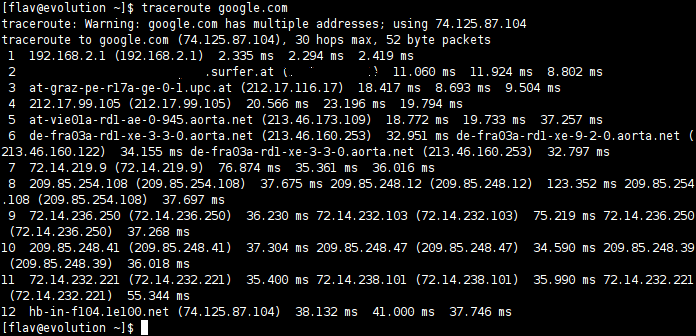
\includegraphics[width=300px]{cap01/traceroute.png}
  \caption{Ruta către un nod}
  \label{fig:cli traceroute}
\end{figure}

După cum vezi, tot ceea ce îi trimit eu lui google.com și ce îmi trimite
el înapoi trece prin alte 11 noduri din rețea. Dacă un \engl{infractor}{cracker}
deține controlul asupra unuia dintre aceste noduri,
poate vedea absolut orice {\glqq}vorbesc{\grqq} eu cu \texttt{google.com}. Un astfel de atac
se numește \href{http://en.wikipedia.org/wiki/Man-in-the-middle_attack}{man in the middle},
deoarece atacatorul se află la mijloc, între
cele două \engl{capete}{endpoints}.

Bineînțeles că nu numai eu aș fi
victima unui astfel de atacator, ci oricine trimite \engl{pachete de date}{data packets}
oricui altcuiva (nu neapărat numai lui \texttt{google.com}), atâta timp cât pachetele
de date trec prin nodul controlat de el.

Toate nodurile din reţeaua globală numită Internet au o adresă unică numită adresă
\engl{IP}{internet protocol}. Ea este de forma \texttt{xxx.xxx.xxx.xxx}, unde \texttt{xxx} este un număr
între 0 şi 255. Unele adrese IP au o semnificaţie specială. De exemplu, fiecare
nod are adresa IP \texttt{127.0.0.1}. Ea nu este utilă în Internet, deoarece orice pachet
de date trimis la acea adresă ajunge înapoi la expeditor, fără nici măcar a trece
pragul sistemului local. Încearcă de exemplu comanda \texttt{tracert 127.0.0.1}.

Alt bloc de adrese IP speciale sunt toate adresele între \texttt{192.168.0.0} şi
\texttt{192.168.255.255}. Ele sunt rezervate \engl{reţelelor locale}{local area network}.\footnote{abv. LAN}

Un astfel de exemplu este chiar reţeaua mea
locală\footnote{Un bun punct de start este \url{http://en.wikipedia.org/wiki/Private_network}.
De acolo poţi urma link-uri intersante către noţiunile ce urmează a fi introduse,
şi multe alte lucruri neprezentate aici.}.
După cum vezi în figura \ref{fig:cli traceroute},
pachetele de date care pleacă de la mine trec mai întâi prin nodul \texttt{192.168.2.1}.
Aceasta este adresa \textsl{router}-ului meu. \textsl{Topologia} reţelei din perspectiva mea
arată ca în figura \ref{fig:topologie}.

\begin{figure}[h]
  \centering
    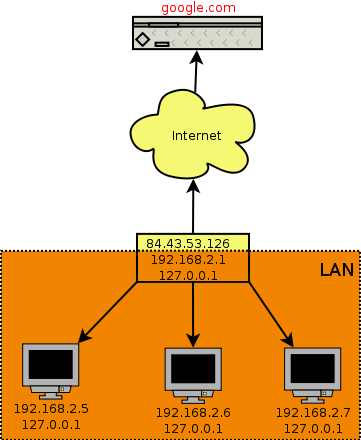
\includegraphics[width=100px]{cap01/Diagram1.png}
  \caption{Exemplu de topologie a unui LAN}
  \label{fig:topologie}
\end{figure}

Misiunea unui \textsl{router} este să distribuie pachetele
pe care le primeşte altor calculatoare din \textsl{LAN}-ul meu. Asta îmi permite să am acces
la Internet cu mai multe calculatoare, însă din exterior \textsl{LAN}-ul este văzut ca
având o singură adresă IP: \texttt{84.43.53.126}, şi deci ca un singur calculator. Dacă
nu puneam acest \textsl{router} între calculatoarele mele şi Internet, nu puteam conecta
la Internet decât un singur calculator, care avea adresa IP \texttt{84.43.53.126}.

\sloppy Există deci două tipuri de adrese IP, cele interne reţelei mele, precum \texttt{192.168.2.1}
sau \texttt{192.168.2.6} şi cele externe reţelei, publice, precum \texttt{84.43.53.126} sau una
dintre adresele lui \texttt{google.com}, \texttt{74.125.87.104}.
Cele dintâi se numesc \textsl{adrese private}\footnote{le poţi numi şi {\glqq}intranet{\grqq},
analog cu cele publice, {\glqq}internet{\grqq}.}
sau adrese LAN, cele din urmă sunt în schimb \textsl{adrese publice}.

\attention{Internetul este o reţea de LAN-uri şi \engl{WAN-uri}{wide area network} interconectate.
Asta transformă Internetul în cea mai mare WAN, o reţea globală.}

Dacă nu ai un \textsl{router} la mijloc, între tine şi Internet, atunci îţi poţi vedea adresa IP
externă prin interfaţa pusă la dispoziţie de sistemul tău de operare. Sub windows, introdu
comanda \texttt{ipconfig /all} în CLI, sub GNU/Linux \texttt{ifconfig -a}.

Dacă însă ai un router la mijloc, şi nu ştii cum să-i accesezi interfaţa de configurare,
atunci trebuie să îi ceri unui alt calculator de pe Internet să-ţi spună ce adresă IP
vede el că ai, pentru că ce vede el va fi mereu adresa ta Internet, externă.

\begin{Exercise}[title={What is my IP Address?},difficulty=1]
Caută pe web cu un motor de căutare \textit{what is my ip address} şi compară
adresa afişată de acea aplicaţie web cu ce adresă IP îţi raportează OS-ul tău.
%Din această comparaţie vei deduce dacă între tine şi Internet se află un router sau dacă eşti conectat direct la Internet.
Ce poţi deduce din această comparaţie?
\end{Exercise}

\section{Domenii}
Teoretic, este suficient să ştii adresa IP a unui nod pentru a comunica cu el. De exemplu,
am aflat că una dintre adresele IP ale lui \texttt{google.com} este 74.125.87.104. Deci putem
intra bine mersi pe adresa \texttt{http://74.125.87.104}.

Însă oamenii nu pot reţine uşor numere. De aceea s-a inventat \engl{DNS}{domain name system},
un sistem care converteşte nume precum \texttt{google.com}, în adrese IP. Atunci când introduci
\texttt{google.com} în browserul tău, acesta trimite o cerere la serverul DNS şi primeşte
înapoi adresele IP asociate cu \texttt{google.com}. Abia apoi se conectează la acea adresă IP,
şi îi cere informaţii.

Sub MS Windows îţi poţi afla serverele DNS cu aceeaşi comandă \texttt{ipconfig} şi parametrul
\texttt{/all}. Sub GNU/Linux, acestea se află în mod normal în fişierul \texttt{/etc/resolv.conf}.

Să presupunem că serverele tale DNS se deconectează de la reţea.\footnote{O glumă
comună este să spui că administratorul serverului s-a împiedicat din greşeală de stecher
şi l-a tras din priză fără să îşi dea seama.} Atunci nu vei mai putea accesa \texttt{http://google.com},
pentru că browserul tău nu mai poate afla adresa IP corespunzătoare. Însă asta nu te împiedică
să introduci manual adresa IP, dacă o ştii.

Pentru a afla dacă un nod este conectat la reţea se foloseşte comanda
\texttt{ping}\footnote{o numim comandă, însă în realitate este un program,
şi se numeşte \texttt{ping.exe}}, având primul
parametru adresa IP pe care vrei să o verifici.

\begin{Exercise}[title={Ping your DNS server}]
Află adresa IP a serverului tău DNS şi trimite-i un pachet de date cu \texttt{ping}.\footnote{Acest exerciţiu nu trebuie
rezolvat în cadrul programului de tutelare, este un exerciţiu suplimentar,
pentru tine.}
\end{Exercise}

Poţi interoga manual serverul DNS cu comanda \texttt{nslookup}
(en. \textsl{nameserver lookup}). Exemple:
\texttt{nslookup google.com}, \texttt{nslookup 192.0.32.10}.
Este deci posibil să afli atât adresele IP pornind de la un nume precum
\texttt{google.com}, însă şi numele, pornind de la o adresă IP de Internet
(nu de intranet).
Deşi este posibil ca mai multe domenii să \textsl{pointeze} către aceeaşi
adresă IP, o adresă IP nu poate {\glqq}pointa{\grqq} (prin \textsl{reverse DNS})
decât spre un domeniu.\footnote{Tehnic este posibil, însă practic poate
cauza probleme.}

Totuşi, din ce este compusă o adresă precum \texttt{www.google.com}?
\texttt{.com} se numeşte \engl{TLD}{top level domain}. Ceea ce se află în stânga
sa este un \textsl{subdomeniu}, până la următorul punct.
Astfel, \texttt{google} este un subdomeniu al lui \texttt{.com},
iar \texttt{www} este un subdomeniu al lui \texttt{.google.com}.

Dacă vrei să ai un domeniu al tău, trebuie să cumperi unul de la
o firmă numită \href{http://en.wikipedia.org/wiki/Domain_name_registrar}{domain name
registrar}. Pentru a învăţa PHP nu ai nevoie de un domeniu, poţi
face totul pe calculatorul tău personal, aşa cum vei vedea în acest capitol.

\section{Protocoale}
Internetul este {\glqq}făcut{\grqq} din aşa-numite \textsl{servicii}. Cele mai cunoscute servicii sunt
web-ul pentru documente interconectate,\footnote{Prin link-uri.}
\textsl{pop3} sau \textsl{imap} pentru e-mail,
\textsl{irc} (en. \textsl{internet relay chat}) pentru chat, sau
\textsl{ftp} (en. \textsl{file transfer protocol}) pentru transferul de fişiere.

Pentru a folosi unul dintre aceste servicii, ai nevoie de un program
special numit \textsl{client}. Nu există un client care să {\glqq}ştie{\grqq} 
să acceseze toate serviciile, pentru
că fiecare serviciu este diferit de celelalte. Vom vedea mai târziu de ce.

Astfel, avem clienţi pentru www, clienţi pentru ftp, clienţi pentru irc, ş.a.m.d.

Serviciul \textit{world wide web}, sau pe scurt \textit{web}-ul, este atât de răspândit, încât
oamenii au dat un nume special clienţilor www: \textsl{browser}. Există mai multe browsere,
create de diferite firme. Printre cele mai cunoscute se numără:
\begin{itemize}
\item \href{http://en.wikipedia.org/wiki/Firefox}{Firefox}, creat de Mozilla
\item \href{http://en.wikipedia.org/wiki/Internet_explorer}{Internet Explorer}, creat de Microsoft
\item \href{http://en.wikipedia.org/wiki/Opera_(web_browser)}{Opera}, creat de Opera Software
\item \href{http://en.wikipedia.org/wiki/Chrome_(web_browser)}{Google Chrome}, creat de Google
\item \href{http://en.wikipedia.org/wiki/Safari_(browser)}{Safari}, creat de Apple
\end{itemize}

Colocvial vorbind, te poţi referi la client şi
ca fiind calculatorul pe care rulează clientul, sau chiar la utilizatorul uman din spate
care îi dă instrucţii clientului. În explicaţii voi încerca să nu mă exprim colocvial, ci
corect din punct de vedere tehnic.

În continuare vom clarifica ce se întâmplă atunci când ceri o pagină web cu ajutorul
unui browser de la un server.

Imaginează-ţi că un calculator stă conectat la reţea şi
nu face nimic din {\glqq}proprie iniţiativă{\grqq}.
Acest calculator se numeşte \textsl{server}. Pe server, care este
\textit{maşina fizică}, rulează \textit{un program} numit \textsl{daemon}.
Acesta aşteaptă conexiuni din
exterior, pe care să le deservească. Administratorul serverului va spune colocvial
\textit{the server is up and running}, dar ce vrea să spună de fapt este că \textit{serverul
este conectat la Internet iar cel puţin un daemon aşteaptă noi conexiuni}.

Să nu uităm că fiecare serviciu este diferit. Aşa cum avem diferiţi clienţi pentru
diferite servicii, tot la fel avem şi \textit{daemon}-uri diferite pentru fiecare serviciu.

Exemple de astfel de \textit{daemon}-uri: \textsl{apache} pentru serviciul
www, \textsl{UnrealIRCd} pentru irc,
\textsl{postfix} pentru e-mail, ş.a.m.d. Reţine că acestea sunt programe, la fel
cum este şi \texttt{firefox.exe}. În contrast cu asta noţiunile de \textit{client} şi
\textit{daemon} sunt clasificări
generice pentru tipuri de software.

Ceea ce nu am încetat să sugerez până acum devine evident: cele două părţi, clientul
serviciului pe care doresc să-l utilizez, şi daemonul care e capabil să-i răspundă
clientului meu cu informaţii utile, trebuie să comunice unul cu celălalt.

Această comunicare dintre cele două programe se va desfăşura într-un limbaj comun numit
\textsl{protocol}. Fiecare serviciu are un protocol specific lui. Astfel avem un
protocol irc pentru serviciul irc, protocolul ftp pentru serviciul ftp,
sau protocolul http pentru serviciul web, ș.a.m.d. De aici vine acel {\glqq}http://{\grqq} care precede
orice adresă web. Această adresă se numeşte
\engl{\href{http://en.wikipedia.org/wiki/Uniform_Resource_Locator}{URL}}{uniform resource locator},
o formă de \engl{\href{http://en.wikipedia.org/wiki/Uniform_Resource_Identifier}{URI}}{uniform resource identifier}.

De obicei pe un server rulează mai multe \textit{daemon}-uri în paralel şi care
aşteaptă să deservească cereri. Dar cum să ştie sistemul de operare al serverului
pentru ce daemon este destinat un anumit pachet de date? Din câte ştim până acum,
nu are cum, pentru că OS-ul nu înţelege noţiunea de {\glqq}protocol{\grqq}. Totuşi OS-ul trebuie
să paseze datele primite pachet cu pachet daemon-ului corect.

Pentru a rezolva această problemă fiecare pachet de date este {\glqq}însemnat{\grqq} cu un \textsl{port}.
Un port este un număr între 1 şi 65535 care îi permite sistemului de operare să
paseze pachetul de date procesului\footnote{Un program care este executat. Gândeşte-te
la ce listează {\glqq}task manager{\grqq}.} corect.

Atunci când \engl{administratorul serverului}{sysadmin} lansează în execuţie un daemon,
acesta îi spune OS-ului că \engl{ascultă}{listen}
pe un anumit port. Din acel moment, OS-ul
{\glqq}ştie{\grqq} că acel port îi {\glqq}aparţine{\grqq} acelui daemon. Astfel, sysadmin-ul poate rula
pe sistemul său mai mulţi daemoni concomitent, chiar şi pentru servicii diferite, fără
a-şi face griji că pachetele de date ar putea ajunge la daemon-urile greşite.

Important de menţionat este şi că fiecare serviciu are un port standard. Serviciul www
are 80 ca port standard. Astfel, URL-urile \texttt{http://example.com:80} şi
\texttt{http://example.com} sunt absolut echivalente.

În toate cele explicate până acum nu am intrat în detalii importante precum
\href{http://en.wikipedia.org/wiki/Internet_Protocol_Suite}{TCP/IP}, însă este recomandată citirea şi
înţelegerea acelor noţiuni, cât şi a celorlalte articole pe care le poţi urma de acolo.
Foarte importantă este şi înţelegerea modelului
\engl{\href{http://en.wikipedia.org/wiki/OSI_model}{OSI}}{open system
interconnection}.

\subsection{Primul exerciţiu de hacking}

Înainte de a trece la conţinutul propriu-zis, vreau să clarific de ce această secţiune
foloseşte termenul \textsl{hacking}.

În primul rând, pentru a face acest capitol mai
atractiv pentru toţi cititorii care s-au plictisit de teoria uscată\footnote{Trebuie să
recunoaştem că nu a fost deloc uscată.} de reţelistică
prezentată până acum,
când ei vor de fapt să înveţe PHP. Nu este ceva iluzoriu, ceea ce vei face în continuare
chiar are de-a face cu hacking. Însă hacking implică mult mai multe\footnote{Şi când
spun asta, nu exagerez.}
 cunoştinţe -- paginile
anterioare doar ţi-au prezentat sumar nişte concepte de bază.

În al doilea rând, pentru a-mi crea ocazia de a explica termenul de hacker.
În zilele noastre, \textsl{mass-media}, în încercarea sa de a crea\footnote{În
sensul de {\glqq}a inventa{\grqq}} senzaţionalul,
a redefinit \textsl{hacker} ca \textit{infractor}. Însă nu asta este semnificaţia
originală a cuvântului. Un hacker este o persoană care înţelege foarte bine ce
face. Poţi fi un hacker în orice domeniu, dar atunci când devii un hacker într-un domeniu,
ştii tot ce mişcă în branşa ta. Un hacker în calculatoare ştie totul despre calculatoare,
începând de la electronica procesorului, şi terminând cu analiza psihologică a
omului în relaţia sa cu
calculatorul (sau, pe larg, cu tehnologia în general).\footnote{Cel mai renumit exemplu este
\href{http://en.wikipedia.org/wiki/Kevin_Mitnick}{Kevin Mitnick}}

O altă concepţie greşită despre hacking este că înseamnă să intri în sisteme care nu-ţi
aparţin (\textit{să le spargi}). Nu asta caracterizează hackerul, ci după cum am mai spus,
înţelegerea lucrurilor cu care are de-a face. Te poţi numi hacker la fel de bine
dacă personalizezi un program scris de altcineva pentru nevoile tale. În astfel
de cazuri se spune că \textsl{ai hack-uit codul sursă}, că l-ai înţeles mai întâi, pentru
a-l putea modifica. După cum vezi, hacking înseamnă \textit{înţelegere}.

Felul în care aplici această înţelegere depinde de tine. Asta nu îi absolvă pe
cei care folosesc ceea ce ştiu pentru lucruri ilegale să fie catalogaţi
drept infractori. Pe de cealaltă parte, hackerii adevăraţi reacţionează acid
când sunt priviţi ca nişte infractori, deoarece ei
ştiu că \textsl{hacking} este de fapt ceva constructiv şi benefic unei minţi sănătoase.
Ei preferă ca infractorii să fie numiţi \textsl{crackeri}, pentru a deosebi binele
de rău.

\vspace{1em}\dotfill\vspace{1em}

Atunci când introduci un URL într-un browser, acesta face multe lucruri în fundal.
Unul dintre cele mai importante lucruri este comunicarea în limbajul
\engl{HTTP}{hyper text transfer protocol} cu \textit{daemon}-ul de pe serverul dorit,
asta după ce a aflat adresa IP a acestuia de la serverul DNS.

Noi vrem să facem manual ceea ce ar face un browser automat pentru noi. Pentru asta,
avem nevoie de un program numit \texttt{telnet}. Este un program foarte simplu, tot ce
face este să stabilească o \textsl{conexiune} cu daemonul, şi să-i transmită datele pe care
le tastăm.

O dată ce conexiunea este stabilită, ambele endpoints (daemonul şi noi, cu ajutorul
clientului telnet) pot scrie la grămadă date. De exemplu dacă noi scriem
\begin{verbatim}
foo
\end{verbatim}
şi daemonul ne răspunde cu
\begin{verbatim}
bar
\end{verbatim}
atunci toate datele comunicate arată ca un fişier cu conţinutul:
\begin{verbatim}
foo
bar
\end{verbatim}

Imaginează-ţi că două endpoints comunică prin plicuri.
Programul care iniţiază conexiunea (numit client), scrie datele pe
care urmează să le trimită într-un plic.

Dacă clientul şi daemonul doar schimbă date {\glqq}aşa cum sunt{\grqq},
aşa cum am face cu telnet, atunci doar acest plic este necesar.
Însă dacă aplicaţiile vor să se înţeleagă reciproc,
ele trebuie să folosească un protocol de comunicare.
Pentru web, acest protocol este HTTP.

Acest protocol de comunicare constituie \textit{layer}-ul \textsl{application level}
din \href{http://en.wikipedia.org/wiki/OSI_model}{modelul OSI}.\footnote{\url{http://en.wikipedia.org/wiki/OSI_model}}

În astfel de cazuri, clientul va trebui să pună în plicul nostru încă
un plic\footnote{sau mai multe, în funcţie de protocolul de comunicare folosit}
cu datele structurate specifice protocolului folosit,
în cazul nostru cele specifice protocolului HTTP.

Majoritatea sistemelor de operare moderne vin cu programul telnet preinstalat.
Deci deschide interfaţa CLI şi lansează programul, pasându-i ca prim parametru numele
serverului, şi \textit{port}-ul ca al doilea parametru, deci:
\begin{alltt}
telnet example.org 80
\end{alltt}
După ce s-a conectat, îi poţi cere daemonului ce document vrei, însă trebuie
să o faci în limbajul HTTP, altfel nu va {\glqq}înţelege{\grqq} ce vrem de la el.
Altfel spus, folosind analogia cu plicul, noi ca oameni, deoarece
ştim că vrem să comunicăm în HTTP, şi deoarece telnet nu are noţiunea
de \textit{application layer}, avem responsabilitatea de a ne
{\glqq}împacheta{\grqq} singuri cererea în încă un plic cu formatul specific HTTP,
plic pe care i-l pasăm lui telnet, care ne va pune plicul
pe rând în toate celelalte \textit{layere} ({\glqq}plicuri{\grqq}) din modelul OSI aflate
sub \textit{application layer}: presentation, session, transport, network, iar
electronica (de exemplu placa de reţea) se va ocupa de data link layer şi
physical layer.\footnote{Lucrurile sunt mult mai complexe, telnet
singur nu ar putea face astfel de lucruri fără susţinere
din partea sistemului de operare. Aici am simplificat imaginea
pentru o mai uşoară înţelegere.}

De exemplu, îi vom cere
pagina de start:
\begin{alltt}
GET / HTTP/1.1\Return
Host: example.org\Return
\Return
\end{alltt}
\attention{Simbolul \Return înseamnă că trebuie să apeşi tasta \keystroke{enter}. Deci pentru a
termina cererea HTTP, apeşi de două ori \keystroke{enter} la rând.
Este posibil ca programul tău telnet să nu afişeze ce tastezi. În acest
caz, trebuie să scrii orbeşte, şi să o faci exact ca mai sus, \textit{inclusiv} scrisul cu litere
mari/mici.
}
GET este \engl{metoda HTTP}{http method} pe care o folosim
pentru a cere resursa (documentul) dorit.

Protocolul\footnote{Formatul} HTTP ne dictează că după GET urmează un spaţiu
şi apoi calea către documentul dorit, urmat de protocolul folosit, aici HTTP, un
slash, şi versiunea protocolului.

Prima linie \texttt{GET / HTTP/1.1} se numeşte \textsl{request line}.
După ea urmează o serie de \textsl{request headers}, precum \texttt{Host} mai sus.

Request line şi request headers împreună sunt cunoscute şi ca cererea HTTP (en.
\textsl{HTTP request}).
	
Daemonul îţi va răspunde cu un text care arată cam aşa, şi care constituie răspunsul
HTTP (en. \textsl{HTTP response}):
\begin{Verbatim}[commandchars=\\\{\}]
HTTP/1.1 200 OK
Server: Apache/2.2.3 (Red Hat)
Last-Modified: Tue, 15 Nov 2005 13:24:10 GMT
ETag: {\glqq}b300b4-1b6-4059a80bfd280{\grqq}            
\nl{1}Accept-Ranges: bytes                        
Content-Type: text/html; charset=UTF-8      
Connection: Keep-Alive                      
Date: Tue, 15 Dec 2009 11:52:46 GMT         
Age: 2528                                   
Content-Length: 438

<HTML>
<HEAD>
  <TITLE>Example Web Page</TITLE>
</HEAD>                          
<body>                           
\nl{2}<p>You have reached this web page by typing &quot;example.com&quot;,
&quot;example.net&quot;,                                            
  or &quot;example.org&quot; into your web browser.</p>             
<p>These domain names are reserved for use in documentation and are not available 
  for registration. See <a href={\glqq}http://www.rfc-editor.org/rfc/rfc2606.txt{\grqq}>RFC   
  2606</a>, Section 3.</p>                                                        
</BODY>                                                                           
</HTML>
\end{Verbatim}
Întreaga comunicaţie cu daemonul este deci compusă din trei segmente mari, fiecare separate
printr-o linie goală, rezultată din apăsarea de două ori a tastei \keystroke{enter}:
\textsl{HTTP request}, \textsl{HTTP response headers} (segmentul (1) din outputul de mai sus),
şi \textsl{HTTP response body} (segmentul (2)).

Felul în care se face cererea este parte din specificaţia
limbajului de comunicare HTTP. Acest limbaj, ca şi multe altele, au fost stabilite
prin aşa-numitele \href{http://en.wikipedia.org/wiki/Request_for_Comments}{RFC}-uri
(en. \textsl{request for comments}).

Folosind analogia cu plicurile, cele şapte niveluri din modelul OSI nu sunt totul:
protocolul HTTP însuşi mai defineşte încă trei plicuri care trebuie puse în
{\glqq}plicul{\grqq} cu datele HTTP:
\begin{itemize}
\item \textsl{HTTP request}
%, care conţine la rândul
%său două plicuri: prima linie (cea cu {\glqq}GET{\grqq}) \textsl{request line} şi
%\textsl{request headers} (precum \texttt{Host:})
\item \textsl{response headers}
\item \textsl{response body}
\end{itemize}
Chiar dacă cele trei {\glqq}segmente{\grqq} sunt scrise fie de client, fie de daemon,
noi privim \textit{întreaga comunicaţie} ca pe un fişier unitar, şi din acest motiv
putem spune că este constituită din aceste trei segmente ({\glqq}plicuri{\grqq}).

După ce a primit răspunsul HTML, un browser ar face alte lucruri precum:
\begin{itemize}
\item crearea de cereri noi pentru fiecare element care face referire la resurse
externe precum imagini, frame-uri, scripturi Javascript, ş.a.m.d. În urma 
acestui pas imaginile ar părea că fac parte din document, însă ele sunt de fapt
resurse diferite şi de sine stătătoare, cu URL-uri diferite.
\item executarea scripturilor Javascript
\end{itemize}

Deoarece pentru fiecare resursă externă este necesară crearea unei noi conexiuni
TCP/IP şi comunicarea cu serverul în limbajul HTTP, protocolul HTTP este
un \textsl{protocol stateless}\footnote{\url{http://en.wikipedia.org/wiki/Stateless\_protocol}}.


\begin{Exercise}[title={HTTP e stateless}]
Faptul că HTTP este un protocol stateless are implicări majore asupra
structurii fundamentale în care îţi vei concepe aplicaţiile.

Gândeşte-te la aceste implicări şi explică-le în 200-300 cuvinte.
\end{Exercise}

Însă clientul nostru telnet nu ştie toate aceste lucruri, el nu înţelege
limbajul de comunicare HTTP pe care l-am folosit,\footnote{Protocolul
de comunicare este {\glqq}plicul{\grqq} ce corespunde \textsl{application layer} în modelul OSI.}
cum nu înţelege nici limbajul
de formatare HTML, în consecinţă nici nu poate afişa imagini sau executa scripturi Javascript.
El doar s-a conectat la daemon pe portul dorit de noi, şi ne-a oferit posibilitatea
de a comunica cu el în HTTP pentru a primi codul HTML al paginii.

Dacă în acest moment am vrea să cerem daemonului un alt fişier, şi nu cel standard,
ar trebui să nu-i cerem resursa {\glqq}/{\grqq} (care urmează după {\glqq}GET{\grqq} în cererea anterioară,
şi care este numită şi \textsl{root}),
ci numele resursei cu tot cu calea sa absolută. De exemplu, pentru fişierul
{\glqq}http://example.org/contact.html{\grqq},
cererea ar arăta astfel:

\begin{verbatim}
GET /contact.html HTTP/1.1
Host: example.org

\end{verbatim}

Motivul pentru care trebuie să specificăm la ce domeniu ne referim în câmpul
(en. \textsl{header field}) \textsl{Host} (aici: \texttt{example.org}) este că un daemon HTTP
poate deservi mai multe domenii simultan, şi deci trebuie să-i spunem la care
din ele ne referim.
De exemplu, este posibil ca \texttt{http://example.org} şi
\texttt{http://www.example.org} să fie două site-uri complet diferite, independente, cu
fişiere diferite. Întâmplător, administratorul care a setat acel apache 2.2.3 (ştim că
acel program cu acea versiune deserveşte acel site din response header-ul {\glqq}Server{\grqq}) a făcut setările astfel
încât cele două hostname-uri complet diferite \texttt{example.org} şi \texttt{www.example.org}
să facă referire către acelaşi director de pe server. Din acest motiv nu contează
către ce hostname trimitem cererea, daemonul ne va răspunde cu aceleaşi fişiere.

\section{Instalarea mediului de dezvoltare}
În această secţiune vom instala cele două scule necesare creării şi testării
aplicaţiilor web, sau mai bine spus, scripturilor PHP. Mă voi limita doar
la instrucţiuni
pentru Microsoft Windows XP. Instalarea sub GNU/Linux este uşoară: nu trebuie
decât să instalezi pachetele de genul \texttt{apache} sau \texttt{httpd}
şi \texttt{PHP} din repozitoriul
pus la dispoziţie de distribuţia ta, aşa cum ai instala orice alt program.
Directivele de configurare sunt foarte similare, deci o citire a instrucţiunilor
următoare nu este de prisos, chiar dacă foloseşti GNU/Linux.

Paşii şi instrucţiunile de configurare sunt aceeaşi,
atât pentru windows, cât şi pentru GNU/Linux.

În primul rând, intră pe pagina oficială a daemonului
apache\footnote{\url{http://httpd.apache.org/}} şi urmează linkul
Download a ultimei versiuni, momentan\footnote{17.01.2010} 2.2.14.


\begin{figure}[h!]
  \centering
    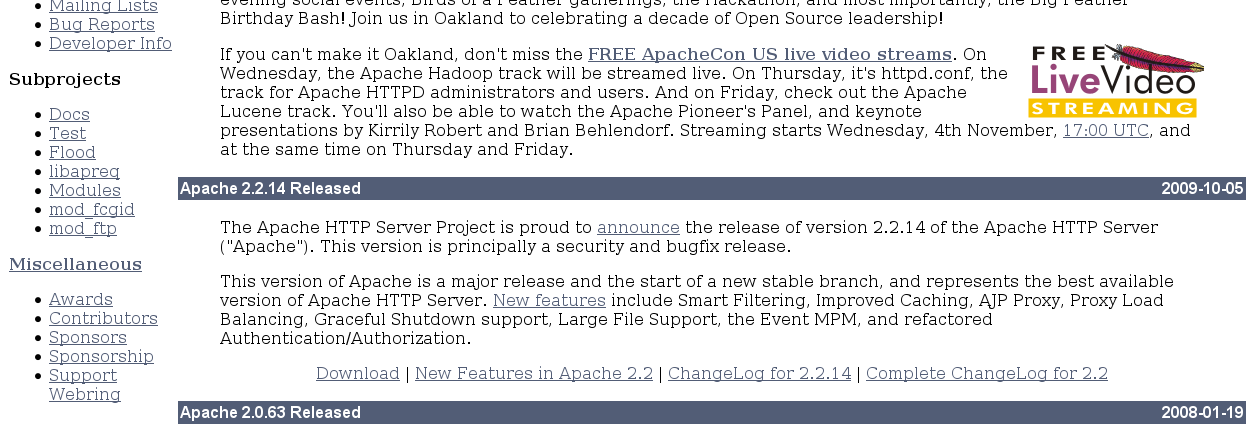
\includegraphics[width=400px]{cap01/Screenshot.png}
  \caption{Pagina oficială Apache HTTPD}
  \label{fig:httpd homepage}
\end{figure}


Alege un \textsl{mirror}\footnote{
Un mirror este o oglindire a unor fişiere. Mai multe firme sau instituţii au ales
să pună la dispoziţie oglindiri ale fişierelor de instalare pentru apache. Oricine
poate face un mirror, însă e recomandat să înştiinţezi autorul oficial, pentru
ca acesta să pună un link către mirror-ul tău. Toate fişierele de pe un mirror sunt identice,
deci teoretic nu contează ce mirror alegi, însă este recomandat să alegi un mirror
apropiat ţie din punct de vedere geografic, pentru ca descărcarea să fie mai
rapidă.} şi apasă \texttt{change}. Mirror-ul selectat automat ar trebui să fie unul
dintre cele mai bune. Apoi selectează versiunea {\glqq}Win32 Binary without crypto{\grqq}.

%\begin{figure}[h!]
%  \centering
%    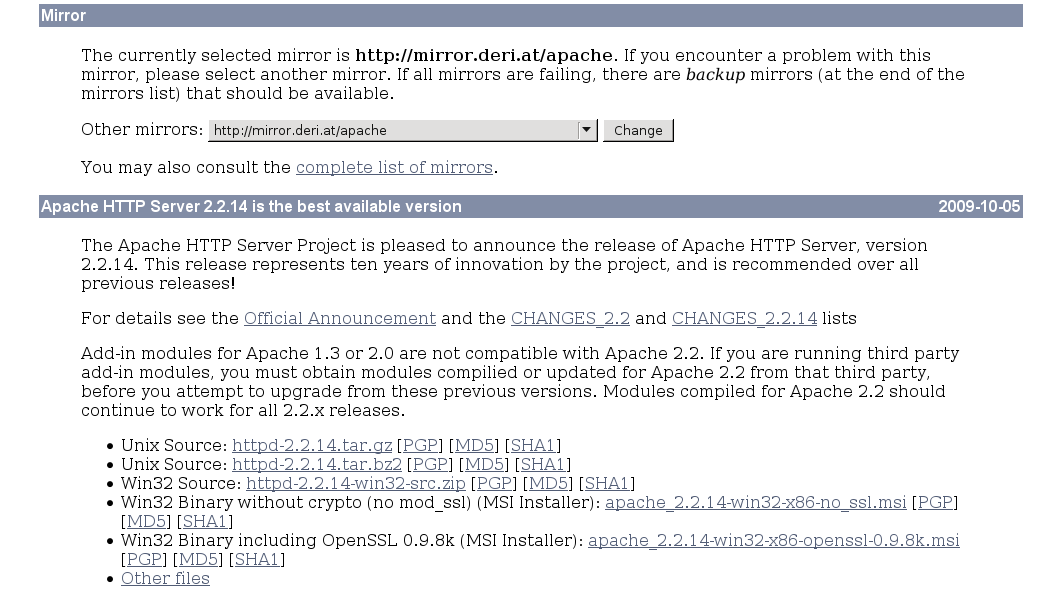
\includegraphics[width=400px]{cap01/Screenshot-1.png}
%  \caption{Setarea iniţială apache httpd}
%  \label{fig:httpd setup}
%\end{figure}

Introdu datele ca în figura \ref{fig:httpd setup} şi treci la pasul următor.

\begin{figure}[h!]
  \centering
    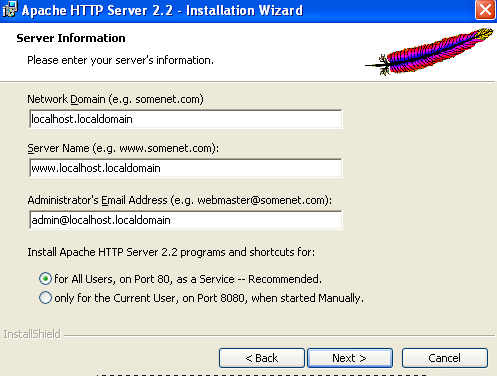
\includegraphics[width=300px]{cap01/Screenshot-2.png}
  \caption{Setarea iniţială apache httpd}
  \label{fig:httpd setup}
\end{figure}

Alege modul de instalare \texttt{custom}, deoarece vrem să decidem exact unde şi ce
se instalează, ca în \ref{fig:httpd check custom setup}.

\begin{figure}[h!]
  \centering
    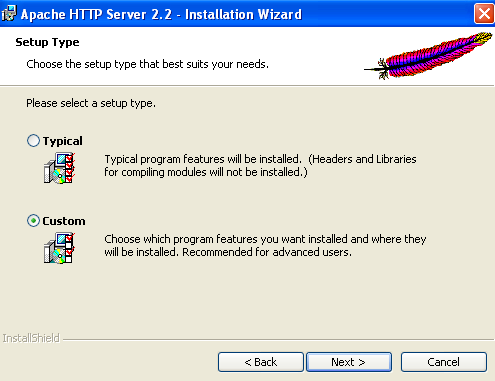
\includegraphics[width=250px]{cap01/Screenshot-3.png}
  \caption{Setare personalizată}
  \label{fig:httpd check custom setup}
\end{figure}

În figura \ref{fig:httpd components tree} avem un arbore cu toate componentele instalate. \texttt{Apache HTTP Server 2.2.14}
este părintele tuturor componentelor. Selectează-l şi apasă pe butonul
\texttt{Change...} pentru a schimba locul de instalare.

\begin{figure}[h!]
  \centering
    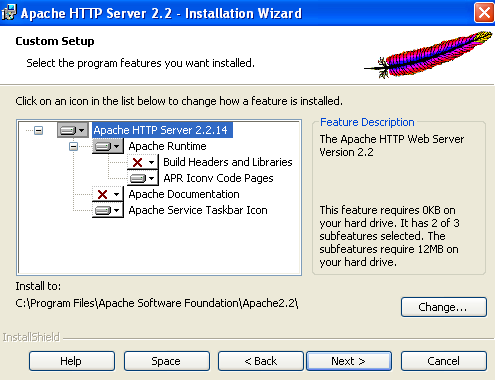
\includegraphics[width=248px]{cap01/Screenshot-4.png}
  \caption{Setare httpd - Componentele instalate}
  \label{fig:httpd components tree}
\end{figure}

Crează un nou director \texttt{C:{\textbackslash}webdev\textbackslash}
unde vor fi instalate toate sculele
de programare web, introducând manual calea \texttt{C:{\textbackslash}webdev{\textbackslash}apache}
exact ca în \ref{fig:httpd custom path}.

\begin{figure}[h!]
  \centering
    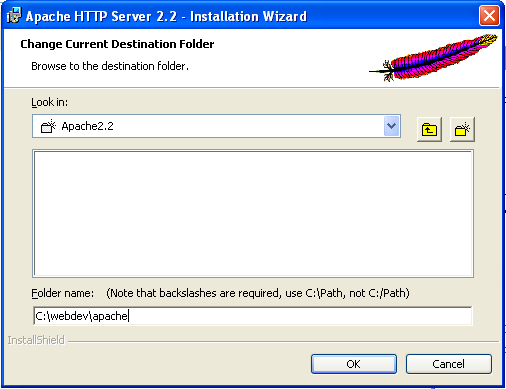
\includegraphics[width=253px]{cap01/Screenshot-5.png}
  \caption{Setare httpd - Calea instalării}
  \label{fig:httpd custom path}
\end{figure}

Confirmarea te va aduce la dialogul anterior, iar în partea de jos ar trebui să scrie
că programul va fi instalat la acea locaţie.

Finalizează instalarea. La vizitarea adresei \url{http://localhost/} ar trebui să
vezi mesajul \texttt{It works!}. Asta înseamnă că daemonul apache este setat corect şi poate deservi
pagini statice în formatul html, iar calculatorul tău este acum un server.

Noi însă vrem să generăm în mod dinamic cod HTML cu PHP. Deci intră pe pagina oficială
PHP\footnote{\url{http://php.net}} şi urmează linkul de download,
sub \texttt{Windows binaries} (Figura \ref{fig:php win bin}).

\attention{Toate programele care lucrează cu text, precum editoarele text şi browserele,
oferă o funcţionalitate de căutare a unui text. În majoritatea programelor, combinaţia
de taste \keystroke{CTRL+F} deschide un dialog de căutare. Fiind pe o pagină,
dacă nu găseşti un text, apasă această combinaţie de taste şi introdu titlurile
linkurilor sau orice alt text în a cărui căutare eşti.}

\begin{figure}[h!]
  \centering
    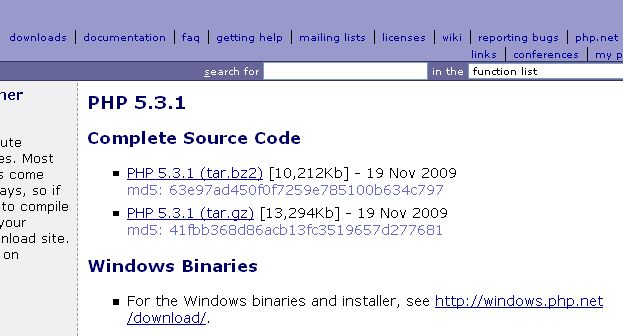
\includegraphics[width=340px]{cap01/Screenshot-6.png}
  \caption{PHP - Pagina oficială de download}
  \label{fig:php win bin}
\end{figure}

Selectează tipul de executabil \texttt{VC6 x86 Thread Safe}, ca în \ref{fig:php build type}, apoi
descarcă arhiva .zip care conţine PHP, salvând-o în \texttt{C:{\textbackslash}webdev\textbackslash}.
\begin{figure}[h!]
  \centering
    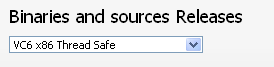
\includegraphics[width=150px]{cap01/Screenshot-7.png}
  \caption{PHP - Tipul \textsl{build}-ului PHP}
  \label{fig:php build type}
\end{figure}


%\begin{center}
%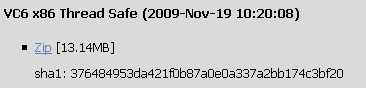
\includegraphics[width=200px]{cap01/Screenshot-8.png}
%\end{center}

După dezarhivare, conţinutul său va arăta ca în Figura \ref{fig:php what you get}.

\begin{figure}[h!]
  \centering
    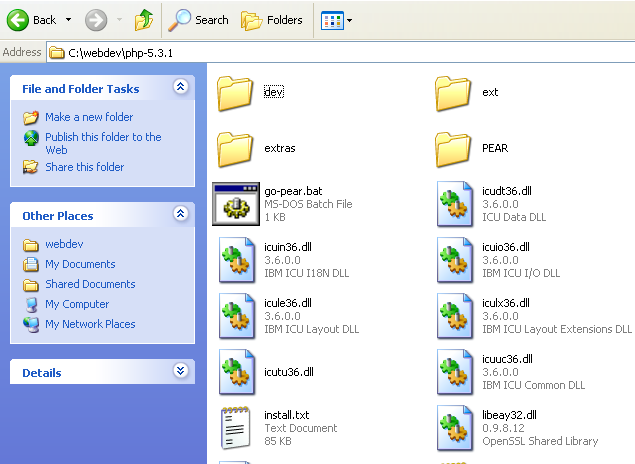
\includegraphics[width=200px]{cap01/Screenshot-9.png}
  \caption{PHP - What you get}
  \label{fig:php what you get}
\end{figure}

Înainte de a trece la integrarea lui PHP în apache, îţi recomand să
instalezi un editor text ideal pentru începătorii în programare:
\href{http://notepad-plus.sourceforge.net/}{Notepad++}
\footnote{\url{http://notepad-plus.sourceforge.net/}}, de pe pagina oficială.
%\begin{center}
%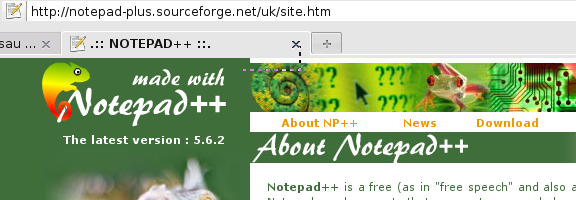
\includegraphics[width=320px]{cap01/Screenshot-10.png}
%\end{center}
%
%Descarcă programul de instalare şi instalează notepad++:
%\begin{center}
%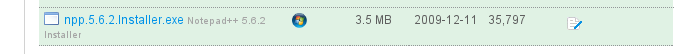
\includegraphics[width=350px]{cap01/Screenshot-11.png}
%\end{center}

\attention{Notepad++ este foarte bun ca editor deoarece, fiind un editor text,
vezi exact ce faci, preluând controlul, aşa cum ar trebui să o facă
orice programator. Pe lângă asta, Notepad++ îţi şi colorează textul
dacă recunoaşte limbajul în care scrii acel text, precum PHP sau HTML.}

\bad{Dacă eşti cumva tentat să foloseşti editoare WYSIWYG\footnote{what
you see is what you get} precum Dreamweaver, atunci ar trebui să
te opreşti acum - programarea nu e pentru tine. De ce? În afară
de faptul că un astfel de editor nu te-ar stimula să înveţi, ţi-ar
şi crea mai multe probleme. Cu PHP, tu ca programator vei prelua
controlul şi vei genera HTML. Pe lânga asta, astfel de programe
nu sunt destul de puternice ca o minte umană, şi mai şi generează
cod greşit.}
\footnotetext{\href{http://en.wikipedia.org/wiki/WYSIWYG}{what you see is what you get}}

PHP poate fi folosit şi ca limbaj de scripting general, nu doar pentru
generarea dinamică de HTML. Însă pentru asta trebuie setată calea
către directorul php care conţine fişierul de configurare \texttt{php.ini},
asupra căruia voi reveni puţin mai târziu.

Sub Windows XP, click dreapta pe \texttt{My Computer} şi apoi \texttt{Properties}.
Sub Windows 7, în \texttt{start} -> \texttt{run} introdu comanda:

\texttt{C:{\textbackslash}Windows{\textbackslash}System32{\textbackslash}SystemPropertiesAdvanced.exe}

Alege tabul \texttt{Advanced}, apoi click pe \texttt{Environment Variables} în partea de jos
a dialogului, aşa cum vezi în Figura \ref{fig:win adv props}.
\begin{figure}[h!]
  \centering
    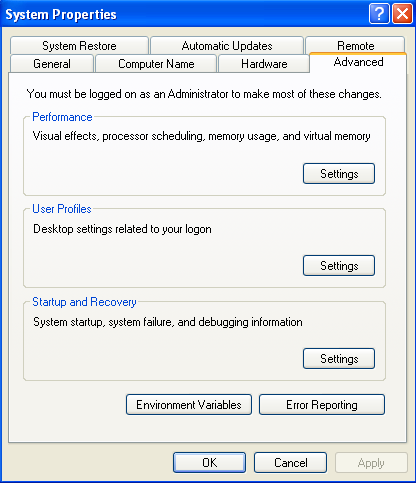
\includegraphics[width=200px]{cap01/Screenshot-12.png}
  \caption{Proprietăţile avansate ale sistemului Windows XP}
  \label{fig:win adv props}
\end{figure}

Se va deschide un dialog similar cu cel din Figura \ref{img:win env vars}.
\begin{figure}[h!]
  \centering
    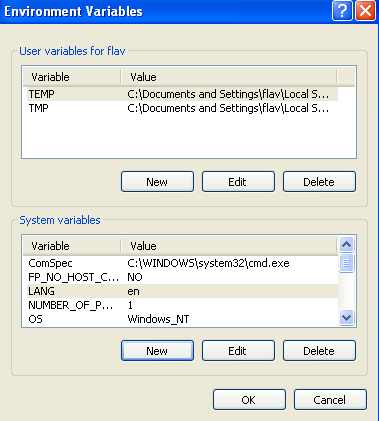
\includegraphics[width=180px]{cap01/Screenshot-13.png}
  \caption{Variabilele de mediu ale unui sistem Windows}
  \label{img:win env vars}
\end{figure}

Click pe \texttt{New} sub \texttt{System variables}, şi introdu datele ca în
Figura \ref{img:win new env var}. Această nouă variabilă de mediu
îl va ajuta pe PHP să-şi găsească fişierul de configurare \texttt{php.ini}.
\begin{figure}[h!]
  \centering
    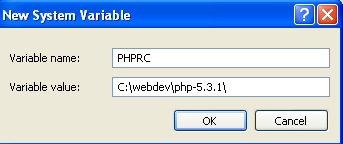
\includegraphics[width=180px]{cap01/Screenshot-14.png}
  \caption{Variabilele de mediu ale unui sistem Windows}
  \label{img:win new env var}
\end{figure}

În acest moment, PHP este setat şi l-am putea lansa în execuţie folosind
calea absolută
\texttt{C:{\textbackslash}webdev{\textbackslash}php-5.3.1{\textbackslash}php.exe}, ceea ce
poate deveni obositor cu timpul. Însă putem integra \texttt{php.exe}
în sistem astfel încât să fie recunoscut ca comandă.

Pentru ca asta să
se întâmple, identifică
variabila systemului numită \texttt{Path}
%\begin{figure}[h!]
%  \centering
%    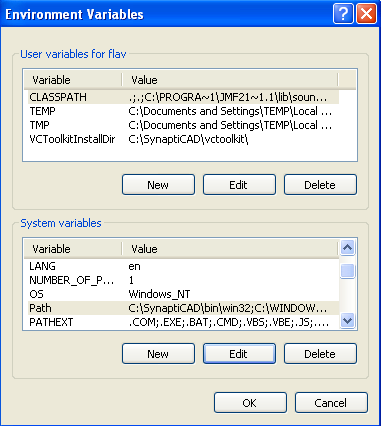
\includegraphics[width=180px]{cap01/Screenshot-20.png}
%  \caption{Variabila de mediu PATH}
%  \label{img:win env path}
%\end{figure}
şi adaugă-i la sfârşit:
\texttt{;C:{\textbackslash}webdev{\textbackslash}php-5.3.1{\textbackslash}}, ca în
Figura \ref{img:win env path}.
\begin{figure}[h!]
  \centering
    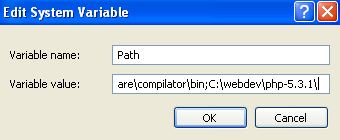
\includegraphics[width=180px]{cap01/Screenshot-21.png}
  \caption{Variabila de mediu PATH}
  \label{img:win env path}
\end{figure}

\attention{Acel ';' de la început este foarte important. \texttt{PATH}
conţine o listă de directoare în care windows se va uita pe rând atunci
când lansezi în execuţie un program ca pe o comandă. ';' are rolul
de a separa aceste directoare.}

Un singur lucru mai lipseşte: \texttt{php.ini}. Arhiva pe care tocmai
ai descărcat-o vine cu două astfel de fişiere, \texttt{php.ini-development} şi
\texttt{php.ini-production}. Fă o \textit{copie} a fişierului
\texttt{php.ini-development} şi redenumeşte-o \texttt{php.ini}.

Testează dacă ai setat totul cum trebuie deschizând o nouă instanţă
a promptului ms-dos.
Acolo introdu comanda \texttt{php --ini}.
Totul este corect dacă php este găsit de sistem, iar comanda de mai sus îţi
arată \texttt{C:{\textbackslash}webdev{\textbackslash}php-5.3.1{\textbackslash}php.ini}
ca \textit{Loaded Configuration File}.

%Mai multe informaţii despre PHP ca limbaj de scripting CLI găseşti pe
%\url{http://www.php-cli.com/}.

\vspace{1em}

Acum vom trece la integrarea lui PHP ca modul apache. Vom spune că folosim
\engl{SAPI-ul\footnote{\url{http://en.wikipedia.org/wiki/Server_Application_Programming_Interface}}}{server application programming interface}
apache2. În directorul în care ai instalat apache este un subdirector de configurare
numit sugestiv \texttt{conf/}, unde rezidă toate fişierele de configurare
pentru apache.

Fişierul principal de configurare se numeşte \texttt{httpd.conf}. Este singurul
fişier încărcat automat de apache pentru a citi configuraţia, celelalte fişiere
trebuie incluse folosind directiva \texttt{Include} din acest fişier
principal (en. \textsl{the master configuration file}). Liniile care încep
cu caracterul diez (\#) sunt comentarii, iar conţinutul lor nu este luat
în considerare, chiar dacă conţine directive de configurare valide.

Deschide \texttt{httpd.conf} cu notepad++ şi adaugă-i la sfârşit
(combinaţia \keystroke{CTRL+END}) directiva
\texttt{Include conf/extra/httpd-php.conf}
apoi crează un nou fişier cu \keystroke{CTRL+N} cu acest conţinut:
\begin{verbatim}
LoadModule php5_module "C:/webdev/php-5.3.1/php5apache2_2.dll"
AddType application/x-httpd-php .php
PHPIniDir "C:/webdev/php-5.3.1"

<IfModule dir_module>
    DirectoryIndex index.php index.html
</IfModule>
\end{verbatim}

Acum apasă \keystroke{CTRL+S} şi salvează-l ca \texttt{httpd-php.conf}
în directorul
C:\texttt{{\textbackslash}webdev{\textbackslash}apache{\textbackslash}conf{\textbackslash}extra{\textbackslash}}

Directiva \texttt{LoadModule} îi spune să încarce un fişier ca modul apache. \texttt{AddType}
îl instruieşte să interpreteze fişiere ce se termină în .php ca 
\texttt{application/x-httpd-php}, care este un tip 
\engl{MIME\footnote{\url{http://en.wikipedia.org/wiki/Multipurpose_Internet_Mail_Extensions}}}{multipurpose internet mail extension}.
\texttt{PHPIniDir} îi spune lui PHP (de data asta modulului PHP) unde îşi găseşte fişierul
de configurare \texttt{php.ini}, aşa cum variabila de mediu \texttt{PHPRC} pe care
am setat-o anterior îi spune acelaşi lucru SAPI-ului CLI (adică lui \texttt{php.exe}).

Acel bloc condiţional\footnote{Se numeşte condiţional deoarece ceea ce se află
în interiorul său este inclus doar dacă condiţia este adevărată, numele însuşi
conţinând \texttt{If}.}
 \texttt{IfModule} verifică dacă apache are modulul {\glqq}dir{\grqq}, şi dacă
da, setează resursa de start corespunzătoare root-ului (atunci când este accesat {\glqq}/{\grqq}
al unui director, aşa cum ai văzut în capitolul anterior) fiecărui director. Fişierele
sunt listate după ordinea priorităţii, dacă primul nu este găsit, apache va încerca să-l
deservească pe al doilea.

\attention{O altă directivă importantă din \texttt{httpd.conf} este
\texttt{DocumentRoot}. Acesta îi spune lui apache de unde
să deservească fişiere. În mod standard, acest director se numeşte
\texttt{htdocs} -- \textsl{hypertext documents}.}

Acum că avem totul setat, restartează daemonul httpd, în caz că e pornit, pentru a prelua
toate schimbările din \texttt{httpd.conf} şi fişierele incluse de acesta. Ar fi trebuit să-i
dăm restart şi dacă am fi modificat configuraţia php din \texttt{php.ini}.

Pentru a verifica instalarea şi configurarea lui PHP ca modul apache, crează un nou fişier
şi salvează-l ca 
\texttt{C:{\textbackslash}webdev{\textbackslash}apache{\textbackslash}htdocs{\textbackslash}info.php}
. Apoi introdu următorul text, numit şi cod sursă (în limbajul PHP):
\lstinputlisting[caption={phpinfo() furnizează toate informaţiile despre instalarea PHP curentă}]{cap01/info.php}
şi salvează-l. 

Acum intră pe adresa \url{http://localhost/info.php}. Ar trebui să vezi ceva similar cu Figura \ref{img:php phpinfo}.

\begin{figure}[h!]
  \centering
    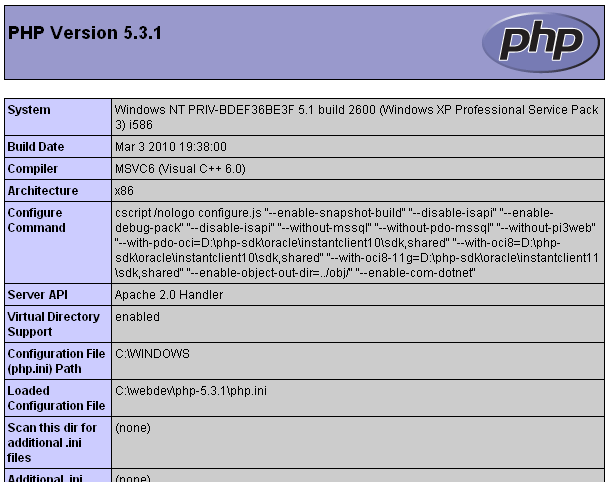
\includegraphics[width=300px]{cap01/Screenshot-15.png}
  \caption{Informaţii afişate de un apel la phpinfo()}
  \label{img:php phpinfo}
\end{figure}

Felicitări, acum ai PHP instalat şi poţi învăţa programare, fie folosindu-l pentru programare web
ca modul apache, fie folosindu-l ca limbaj de scripting universal folosind SAPI-ul CLI. În capitolul următor ne vom uita mai îndeaproape la limbajul PHP.

%variabile, controlul fluxului de executie, input formulare GET
\chapter[Controlul fluxului de execuţie şi de date]{Controlul
fluxului de execuție\footnote{en.
\textsl{execution flow}} și de date\footnote{en.
\textsl{data flow}}}
\vskip -25pt
\textit{Înţelegerea fluxului de execuţie este primordială
în crearea de aplicaţii care fac mai mult decât simple
afişări -- care iau decizii şi îţi fac \textsl{site}-ul dinamic.
Indiferent de cât de simplă sau cât de complexă va fi aplicaţia ta,
indiferent dacă vei folosi baze de date sau simple fişiere,
cu siguranţă vei folosi fluxul de execuţie pentru a controla
fluxul de date. Acest capitol te introduce în lumea datelor,
iar apoi îţi arată cum să le manipulezi.
}

\vskip 5em

%----------------------------------------------------------
\section{O altfel de reîmprospătare}
%\linenumbers

Vreau să stabilesc nişte lucruri care probabil nu sunt evidente
pentru tine, sau asupra cărora nu ai insistat prea mult
când ai început să înveţi să creezi \textit{site}-uri statice
cu HTML, eventual cu CSS sau poate chiar cu interacţiune
în interiorul browserului cu JavaScript.

HTML este un \engl{limbaj de formatare}{markup language}.
Cu el nu controlezi ceva, nu iei decizii, deci nu este
un limbaj de programare. În HTML doar
structurezi un document. În mod ideal îl structurezi
semantic (\href{http://en.wikipedia.org/wiki/Semantic_HTML}{semantic HTML}),
pentru a putea fi interpretat mai bine de motoarele de căutare web
(en. \textsl{search engine}).

Există multe formate de fişiere, şi chiar în capitolul anterior ai
lucrat cu două astfel de formate -- formatul de configurare specific apache, şi protocolul
HTTP. Dacă îţi aminteşti,
ţi-am explicat pe rând ce înseamnă directive precum \texttt{Include}.
Semnificaţia acestor directive, sau general spus, semnificaţia oricărei
entităţi specifice unui limbaj (fie el de markup -- HTML, de configurare
-- \texttt{httpd.conf}, de programare -- PHP, sau un protocol de
comunicare -- HTTP) constituie \textsl{semantica}
acelui limbaj.

Semantica unui anumit construct al unui limbaj (de orice natură
ar fi el) este strâns legată de \textit{contextul} în care se află acel
construct.
De exemplu, pentru a cere o resursă cu HTTP, am văzut că
poţi începe cererea cu GET, urmat
de o cale absolută (care începe cu {\glqq}/{\grqq}) din cadrul \texttt{Host}-ului
în cauză. Calea respectivă are semnificaţia pe care o vrem
doar în contextul lui {\glqq}GET{\grqq}, ca dovadă că atunci când vedem
căi de genul \texttt{/script.php} pe site-uri web,
acestea nu sunt interpretate automat ca parametri GET, şi
deci browserul nostru nu este redirecţionat către acele pagini.

\textsl{Contextul} a ceva înseamnă în ce punem acel ceva pentru a
avea o anumită semantică. De exemplu, sarea pusă în contextul
gătitului are semantica de \textit{condiment}, dar dacă
o pui pe o rană, are semantica de \textit{ceva care provoacă durere}.
Cu alte cuvinte, \textsl{context} înseamnă
\textsl{circumstanţe} sau \textsl{mediul înconjurător}. 

Analog, {\glqq}HTTP/1.1{\grqq} are semantica de {\glqq}protocolul şi versiunea folosită{\grqq}
în contextul \textit{request line}-ului HTTP al unui \textit{request HTTP}.

\begin{Exercise}[title={Întrebări de sinteză},difficulty=2]
Însă şi GET însuşi are semnificaţia pe care ai întâlnit-o în capitolul
trecut doar într-un anumit context semantic.

\Question Care este acest context semantic?
\Question În ce context semantic are semantica întâlnită constructul \texttt{Include}?
\Question În ce context semantic are sens comunicarea în limbajul (în protocolul) HTTP?
\ExeText Determină contextul semantic în care următoarele constructe au semantica pe
care o intuieşti ca cunoscător al limbajului HTML:
\Question <td>
\Question <tr>
\Question <body>
\Question <html>
\Question href
\end{Exercise}


\attention{Dacă ai avut dificultăţi majore la
răspunderea întrebărilor de sinteză, te rog ia atitudine. În primul
rând, plec de la premiza că citeşti cu atenţie, şi că reţii tot
ce-ţi povestesc. Toate noţiunile pe care le introduc, le introduc
pentru că astfel voi putea explica lucruri destul de complicate
mai târziu, pe baza celor spuse aici. \textit{Asta îţi va permite să
ştii multe învăţând cât mai puţin}. {\glqq}Dezavantajul{\grqq} este că
va trebui să fii concentrat la ce citeşti, şi să sintetizezi
singur mult. Sinteza aceasta este un exerciţiu perfect pentru
tine ca viitor programator, deoarece atunci când vei programa
vei fi confruntat cu această nevoie de a sintetiza lucruri.
Metoda mea de predare, deşi dură, te pregăteşte foarte bine pentru
cariera ta de programator. Deci dacă simţi că nu eşti stăpân
pe ce ai învăţat până acum despre reţelistică
şi despre semantică, reciteşte acum, până nu te pierzi definitiv.
Când reciteşti, urmează link-urile menţionate -- după cum am spus
în capitolul Introducere, acestea nu sunt lectură opţională.}

Pe lângă semantică, un limbaj mai are şi o \textsl{sintaxă}. Regulile sintactice
ale limbajelor sunt necesare pentru a crea contextul semantic în
care vor exista constructele acelui limbaj.

Vreau să ilustrez asta cu un exemplu: în protocolul HTTP, GET trebuie
să fie separat de cale printr-un spaţiu. Asta este o regulă sintactică
a limbajului, standardizată prin
RFC-uri,
însă practic separatorul ar putea fi orice altceva.
Însă un separator trebuie să fie acolo, altfel calculatorul (browser-ul
sau daemon-ul) nu ar putea decide unde începe cuvântul cheie {\glqq}GET{\grqq}, unde
se termină, şi unde începe calea către resursa pe care o dorim.
Aceste reguli sintactice
permit programelor precum daemon-uri şi clienţi HTTP
să parseze (să {\glqq}înţeleagă{\grqq}) datele comunicate reciproc.

Există multe posibilităţi de a exprima sintaxa unui limbaj, însă acestea
sunt mult prea complexe pentru noi. Însă există un standard nescris
pentru a specifica sintaxa unor constructe simple, într-o singură linie.
Ea se leagă de necesitatea unui anumit parametru.

De exemplu, sintaxa constructului GET ar putea fi:\\
\begin{verbatim}'GET ' <RESOURCE> ' HTTP/1.1'\end{verbatim}
\texttt{RESOURCE} este pus între < şi >, ceea ce denotă că
este un parametru necesar, care trebuie specificat.
'GET ' (inclusiv spaţiul) şi ' HTTP/1.1' sunt puse
între apostrofuri pentru a arăta că sunt lucruri
ce trebuie scrise exact aşa cum sunt. \texttt{RESOURCE}
este numele simbolic al parametrului, pe care îl putem
refolosi în documentaţia limbajului (în cazul nostru,
documentarea limbajului HTTP, sau mai bine spus, a unei
cereri HTTP de bază).

Pentru a specifica că un parametru e opţional, îl punem între [ şi ].
Astfel, sintaxa unei cereri HTTP ca cea pe care am făcut-o în capitolul
anterior, împreună cu descrierea ei, ar putea arăta astfel:
\begin{verbatim}
'GET ' <resource> ' HTTP/' <version> <enter>
['Host: ' <name enter> ]<enter>

	- resource	= the absolute path to the resource
	- version 	= the version of the HTTP protocol used;
             currently only 1.0 and 1.1 are supported
	- name	    = the hostname
	- enter    = press return once
\end{verbatim}

Pe lângă lucrurile evidente pe care ni le spune această specificaţie
sintactică, ne mai spune şi un lucru care probabil ţi-a scăpat:
câmpul \texttt{Host} este opţional, dar dacă îl specificăm, atunci
trebuie să specificăm şi parametrul \texttt{name}, şi să şi apăsăm o dată enter.

Cu siguranţă ai realizat că astfel de reguli pot fi incluse una în alta,
creând reguli destul de complexe.

Un limbaj precum cel de mai sus, care foloseşte <,>,[,] pentru a specifica
un alt limbaj se numeşte un \textsl{metalimbaj}. \textit{Meta} înseamnă
\textit{care descrie} - \textit{un limbaj care descrie limbajul}.



Cel mai probabil ai întâlnit deja \textsl{tag}-ul HTML \texttt{<meta>}, de aici
îi provine numele. Diferenţa este că \texttt{<meta>} nu se referă la limbaj (HTML
în cazul de faţă), ci la informaţii. Ceea ce \texttt{<meta>} ne spune despre
documentul HTML în care se află se numesc \textsl{metainformaţii} - \textit{informaţii
care descriu informaţiile din documentul curent}.

Probabil ai folosit deja un forum pe web. Probabil că acel forum
îţi spunea la un moment dat că autorul unei intrări (al unui \textsl{topic}
sau \textsl{thread}) se numeşte Xulescu. Ei bine, în timp ce
intrarea propriu-zisă constituie informaţia, numele autorului
este o \engl{metainformaţie}{metadata} - o informaţie despre
informaţie.
%Vom reveni mai târziu asupra conceptului de metainformaţie.

\attention{
La ce îţi foloseşte această cunoaştere despre metadate, metalimbaje, sintaxă
şi semantică? În primul rând, ai învăţat primul cel mai important
lucru pragmatic din viitoarea ta carieră de programator: să citeşti manualul
(PHP sau orice altceva) -- chiar dacă încă
nu eşti conştient de asta.

\smallskip

În al doilea rând, meta-ceva-urile te vor însoţi
în toate aplicaţiile pe care le vei programa. Uită-te
la toate aplicaţiile pe care le foloseşti, vei vedea
că toate au nişte metadate. Singurul lucru care
te-ar împiedica să vezi asta este că datele şi
metadatele se întretaie atât de mult încât e
greu să le identifici pe fiecare.

\smallskip

Şi în al treilea rând, pentru a te pregăti pentru
exerciţiile următoare care au menirea de a te dezgheţa la minte puţin,
deoarece, din păcate, nu ştiu nimic despre cititorul meu, însă trebuie
să mă asigur cumva că este pe aceeaşi lungime de undă ca mine, ceea ce-i
permite să asimileze cât mai eficient cunoaşterea prezentată
în continuare, fără risipă de cuvinte.}

%TODO spune că e un pattern, că 'aba' este potrivit de X Y X, deoarece respectă 'modelul'


\begin{Exercise}[title={Reguli sintactice},difficulty=1]
Fie regula sintactică
%TODO corectează 'A' 'B' 'C'
\begin{verbatim}
                 [A] A [A A] [A [A <B>]] <C>
\end{verbatim}
\ExePart
Care dintre următoarele inputuri o respectă?
\Question AABC % nu
\Question AAAAC % da
\Question AC % da
\Question AAAC % da
\Question AAABC % da
\ExePart
Detaşează-te de această regulă sintactică astractă, şi fă o afirmaţie
\textit{pragmatică} despre B. Afirmaţia începe aşa:
\textit{B este mereu \ldots} % este mereu precedat de cel putin 3, de maxim 6 A-uri
\end{Exercise}

Metalimbajul prezentat nu este bătut în cuie. În primul rând,
caracterele speciale ale limbajului <,>,[,] şi ' pot fi schimbate
în orice, atâta timp cât documentezi aceste schimbări aduse de tine.

Deasemenea, nu este decât un standard nescris, şi îl poţi
extinde în ce fel ai nevoie. Din nou, important este doar
să documentezi {\glqq}extensiile{\grqq} aduse metalimbajului astfel
încât ceilalţi programatori să îţi înţeleagă specificaţia
limbajului pe care îl descrii cu ajutorul acelei
extensii proprii a metalimbajului.

De exemplu, să zicem că vrem să introducem un nou
construct în acest metalimbaj care să însemne \textit{simbolul
din stânga mea poate apărea o dată sau de mai multe ori}, şi
ne decidem să folosim simbolul '+' pentru asta.

Astfel o regulă de genul:
\begin{verbatim}
	<FOO+> [BAR+]
\end{verbatim}
S-ar putea citi ca: \textit{Unul sau mai mulţi \texttt{FOO} urmat de zero sau mai
mulţi \texttt{BAR}}. Un astfel de simbol precum '+' se numeşte \textsl{cuantificator}.
Ar fi la îndemână să stabilim, în documentaţia extensiei noastre adusă metalimbajului,
că '+' poate cuantifica orice entitate din stânga sa, inclusiv o grupare <> sau [].

Documentaţia ar suna aşa:
\begin{verbatim}
+ = repeat the entity on its left once or multiple times (a quantifier)
    the entity can be any SYMBOL, <required parameter> or [optional parameter]
\end{verbatim}
Iar exemplul de mai sus, în care vrem ca \texttt{FOO} şi \texttt{BAR}
să fie separaţi de un eventual spaţiu, ar deveni:
\begin{verbatim}
	<FOO ' '>+ [BAR ' ']+
\end{verbatim}

Până acum definiţiile noastre sintactice se limitau doar la
o singură regulă (o singură linie), însă am putea introduce
constructe în metalimbaj care ne-ar da voie să atribuim nume
acestor reguli, şi să refolosim acele nume în definiţiile altor
reguli sintactice, creând astfel interdependenţe între reguli,
şi deci crea specificaţiile unor limbaje foarte complexe.

\attention{Majoritatea limbajelor de programare, inclusiv
PHP, sunt definite în astfel de limbaje.}

\begin{Exercise}[title={Sintaxa HTML},label={ex:sintaxa_html},difficulty=3]
Acum hai să aplicăm ce am învăţat asupra limbajului HTML. În HTML avem
tag-uri (ex. \texttt{<html>}) care au atribute şi valori.

\Question Crează o specificaţie sintactică a limbajului HTML folosind
doar cuvintele cheie TAG, ATTRIBUTE şi VALUE, care combinate
cu [] şi <> să reflecte cât mai corect sintaxa limbajului.

Specificaţia trebuie să valideze orice text HTML valid.
Un exemplu de input ar fi:
\begin{verbatim}
<form method="get">
   <checkbox name="hello" checked>
   <input type="submit">
</form>
\end{verbatim}
\ExeText
Note:
\begin{itemize}
\item Regula creată \textit{nu} trebuie să ia în calcul sintaxa
specifică XHTML (în care de exemplu '<img>' ar fi greşit, doar '<img />' este valid).
\item Se pleacă de la premiza că inputul este cel mai curat HTML posibil, că
sunt folosite " pentru a delimita valorile atributelor (dacă acestea există), că
nu e mai mult de un spaţiu acolo unde e nevoie de spaţiu, ş.a.m.d. Pe scurt:
foloseşte-ţi intuiţia pentru a decide ce înseamnă {\glqq}cel mai curat HTML posibil{\grqq}.
\item Deoarece caracterele < şi > au o semnificaţie specială în limbajul HTML, pe
care încerci să-l descrii sintactic folosind printre altele
şi caracterele < şi > înseşi, va trebui să le pui între apostrofuri, pentru a face
diferenţa între <,> care ne spun în metalimbajul nostru
că acel parametru este necesar, şi '<' sau '>' care
ne spun că ne referim la caracterul '<' respectiv '>' în limbajul pe care
vrem să-l descriem (adică HTML îsuşi).
\item Va trebui să extinzi metalimbajul (nu uita să şi documentezi extensiile aduse)
pentru a ajunge la o rezolvare cât mai corectă şi completă
\item Exerciţiul este destul de dificil. Încearcă să te apropii cât mai mult de soluţia
cea mai corectă şi completă.
\end{itemize}
\end{Exercise}

%----------------------------------------------------------
\section{Output simplu}
\label{sec:output simplu}
La sfârşitul capitolului anterior, ai făcut cunoştinţă
cu primul tău cod PHP:
\lstinputlisting{cap01/info.php}

Prima linie marchează începutul procesării PHP. Ce se află
înaintea \texttt{<?php} este trimis aşa cum este către client.
Hai să testăm. Scrie ceva în tagul <h1> înainte de începutul
procesării PHP şi vezi ce iese:
\lstinputlisting{cap02/1-helloinfo.php}

PHP generează prea mult cod HTML pentru gusturile noastre simpliste, deci
fă cunoştinţă cu un cuvânt cheie în PHP: \texttt{echo}. Sintaxa
generală este:
\begin{verbatim}
echo <EXPR>;
\end{verbatim}
unde \texttt{EXPR}  trebuie să fie o expresie care evaluată, se reduce la o valoare.

\attention{Nu te speria dacă nu înţelegi totul, voi reveni asupra subiectului. Deocamdată urmează pur şi simplu paşii prezentaţi de mine, respectând sintaxa.
Simte-te liber să faci modificări, să experimentezi. Dacă faci ceva ce generează
o avertizare sau o eroare nu te impacienta, citeşte-o cu atenţie, încearcă
să o înţelegi, şi cere lămuriri pe wiki-ul proiectului.
}

Hai să-l învăţăm pe PHP să ne salute. În notepad++ crează un nou fişier
şi salvează-l ca \texttt{salut.php} în htdocs, apoi introdu codul:
\begin{lstlisting}
<?php
echo 'Salut Flavius';
\end{lstlisting}
Acum fă cu telnet o cerere HTTP, să vezi exact ce se întâmplă atunci când
interpreterul PHP execută acel cod:
\begin{verbatim}
GET /salut.php HTTP/1.1
Host: localhost
\end{verbatim}

Ce observăm? Exact! Observăm că nu vedem nici urmă de cod PHP, vedem doar
outputul generat de el. Nu tu \texttt{<?php}, nu tu \texttt{echo}. Asta
ne demonstrează că PHP ne-a procesat scriptul, script care a generat
output. Dacă scriptul nu ar fi generat output, \textit{response body}-ul
HTTP ar fi fost gol.

În al doilea rând, \textsl{http response body} nu conţine date în format HTML.
De ce? Simplu, deoarece nu i-ai spus niciunde să genereze nimic ce ar putea arăta a
HTML. Cum facem asta? O posibilitate ar fi următoarea:
\begin{lstlisting}
<?php
echo '<html><body>';
echo 'Salut Flavius';
echo '</body></html>';
\end{lstlisting}

Concluzia pe care o tragem este că PHP habar n-are ce este HTML. De ce?
După cum am spus atunci când ai instalat CLI-ul PHP (numit \texttt{php.exe}),
PHP este un limbaj de scripting general. De fapt nu este legat în niciun mod de
HTML sau de site-uri. Este doar felul în care îl folosim noi şi majoritatea
restului lumii. De fapt, PHP poate genera orice, imagini, documente, animaţii
(flash). Chiar nu eşti restrâns la HTML, dar nici nu te ajută în acest sens --
trebuie să scrii manual codul HTML, după cum ai văzut mai sus.

Vei vedea însă că îţi pune la dispoziţie constructe care înlesnesc generarea
de HTML -- de exemplu poţi genera o galerie de imagini aflate într-un anumit
director pe server, fără să trebuiască să ştii dinainte numele fişierelor.

Totuşi exemplul nostru anterior nu prea are sens -- nu este nimic dinamic în el.
L-am putea rescrie la fel de bine doar în HTML static, însă deoarece
vreau să demonstrez altceva, voi genera totuşi mesajul de salut cu PHP:
\begin{lstlisting}
<html>
	<body>
		<?php
		echo 'Salut Flavius';
		?>
	</body>
</html>
\end{lstlisting}

Observi că pentru a termina procesarea PHP şi a afişa din nou totul
aşa cum este (en. \textsl{unparsed}) se foloseşte \texttt{?>}.
În acest mod poţi porni şi opri procesarea PHP de oricâte ori doreşti în acelaşi fişier.
La sfârşitul fişierului procesarea este terminată automat, de aceea în exemplele
anterioare nu a fost nevoie de {\glqq}?>{\grqq}.

\attention{Mai observă şi cum mi-am făcut codul uşor de citit \textsl{indent}ându-l (en.
\textsl{to indent}), adică am aliniat deschiderea fiecărui tag HTML cu tag-ul
de închidere corespunzător, făcându-mi codul lizibil. Pentru codul nostru sursă
minuscul nu prea contează, însă diferenţa de mentenabilitate va fi
vizibilă când fişierele vor avea sute sau mii de linii de cod (LOCs en.
\textsl{lines of code}). Deci obişnuieşte-te
să indentezi codul apăsând tasta \keystroke{TAB} pentru fiecare nou nivel de
indentare necesar.}

Din acest punct înainte scopul nostru este să învăţăm PHP, nu să generăm
cod HTML valid, deci nu ne vom mai obosi să decorăm textul generat
cu \texttt{html} sau \texttt{body}. Însă nu uita că într-o pagină HTML
normală, validă, şi asta trebuie făcut, eventual
punând şi un
\textsl{doctype}\footnote{
\href{http://en.wikipedia.org/wiki/Document_Type_Declaration}{document type declaration}}, altfel
browserul intră în \href{http://en.wikipedia.org/wiki/Quirks_mode}{quirks mode}.

%----------------------------------------------------------
\section{Folosirea variabilelor}
Înainte de a trece la noţiuni noi, trebuie să revenim asupra exemplului nostru
cu câteva completări:
\begin{lstlisting}
<?php
echo 'Salut Flavius';
\end{lstlisting}
Ştim deja că \texttt{echo} este un cuvânt cheie care generează output pe baza
primului său parametru. Sper că ai intuit deja că fiecare instrucţiune
trebuie separată de următoarea prin ';'.

Însă ce este 'Salut Flavius'? Este o valoare în primul rând, pentru că
i-o putem pasa lui \texttt{echo}. În al doilea rând, este o constantă,
deoarece nu se modifică. La fiecare interpretare a scriptului, \textit{output}-ul
va fi acelaşi. Sumarizat: este o \textsl{valoare constantă}.

Pe lângă faptul că este o valoare constantă, mai este şi un \engl{şir de caractere}{string}.
Acesta este motivul pentru care
am pus mesajul între apostrofuri -- altfel PHP ar fi încercat să
interpreteze \textsl{Salut} şi \textsl{Flavius} ca constructe ale limbajului,
care evident nu există.

\good{Corect terminologic spunem deci că 'Salut Flavius' este un \textit{string constant} sau
mai pe larg \textit{o valoare constantă de tip string}.}

Deci încearcă! Fă-l pe PHP să genereze erori:
\begin{lstlisting}
<?php
echo Salut Flavius;
\end{lstlisting}
Mesajul de eroare ne-ar putea părea confuz:\\
\texttt{Parse error: syntax error, unexpected T\_STRING, expecting ',' or ';'}\\
Ceea ce se întâmplă este următorul lucru: PHP citeşte \texttt{echo}, şi deoarece a citit
şi a recunoscut instrucţiunea \texttt{echo}, intră în contextul semantic în care se aşteaptă ca următorul
lucru să fie o valoare, însă nu găseşte una, ci întâlneşte \texttt{Salut},
pe care nu-l recunoaşte\footnote{De fapt, parserul se blochează la {\glqq}Flavius{\grqq}, însă
ca să explic asta cum trebuie, ar fi trebuit să fi introdus deja constantele}
ca şi construct al limbajului.
De aceea ne spune că nu se aşteaptă să vadă T\_STRING-ul \texttt{Salut}.

Dar stai puţin, de ce îl numeşte {\glqq}T\_\textbf{STRING}{\grqq}, dar nu îl acceptă ca string?
Pentru a înţelege asta, trebuie să priveşti puţin lucrurile din perspectiva parserului
PHP. Codul sursă pe care îl scriem în limbajul PHP este folosit ca input pentru
parser. Acest input scris de noi este citit de PHP ca string, ca un şir de caractere.
Din acest motiv PHP ne spune foarte corect că nu se aşteaptă să vadă acel string acolo,
ci altceva.
\attention{Pentru PHP, codul scris de noi este un simplu text.}
Hai să vedem ce ar genera PHP dacă nu s-ar aştepta să vadă un string
din perspectiva noastră:
\begin{lstlisting}
<?php
echo 'Salut' 'Flavius';
\end{lstlisting}
ne zice \texttt{Parse error: syntax error, unexpected T\_CONSTANT\_ENCAPSED\_STRING}.

Ce înveţi din asta? În primul rând, înveţi că mesajele de eroare, deşi nedorite,
oferă informaţii preţioase despre ce s-a întâmplat. Din proprie experienţă
pot spune că vederea unui mesaj de eroare sau avertizare e ca o mână cerească,
reversul medaliei fiind mult mai frustrant: să nu vezi o eroare, dar codul
nici să nu funcţioneze aşa cum îţi imaginezi că ar trebui să funcţioneze -- sau
mai rău, să nu afişeze nimic, lăsându-te în întuneric complet. Deci fi fericit
când PHP îţi spune ce ai greşit, caută să înţelegi ce-ţi spune, şi apoi
repară-ţi greşeala.

Pe lângă stringuri, mai există şi alte tipuri de valori constante. PHP înţelege
\engl{numere întregi}{integers}, de exemplu \texttt{42},\footnote{Sunt curios
când va veni cineva să-mi spună de ce am ales 42 :-)}
numere cu virgulă (en, \textsl{floating point numbers} sau scurt \textsl{floats}),
unde partea zecimală
e separată de partea întreagă prin punct, de ex \texttt{3.1415}, şi alte lucruri
asupra cărora vom reveni. Hai să ne uităm la un exemplu:
\begin{lstlisting}
<?php
echo 'Salut 00';
echo 7;
echo '. PI este ~';
echo 3.1415;
\end{lstlisting}

\subsection{Variabile şi tipuri de date elementare}
Toate bune şi frumoase cu lucrurile cu care ai făcut cunoştinţă
până acum, însă ele nu te-au ajutat să creezi ceva dinamic.

Deci hai să facem un pas înapoi şi să ne gândim ce înseamnă şi
ce implică o eventuală dinamicitate. Pentru a fi dinamică, o
pagină trebuie să fie capabilă să primească date de intrare (\texttt{input}),
pentru a genera date de ieşire (\texttt{output}) pe baza acestora.

De exemplu, să zicem că vrem să facem o pagină care în loc să afişeze
mereu {\glqq}Salut Flavius{\grqq}, afişează {\glqq}Salut <nume>{\grqq}. Acest input (numele) trebuie
salvat undeva, altfel nu avem acces la el. Bine ai venit în lumea variabilelor.

O variabilă are trei caracteristici
\begin{enumerate}
\item un \textsl{nume} sau \textsl{identificator}
\item o \textsl{valoare} pe care o ţine
\item \textsl{tipul de date} (en. \textsl{datatype}) al valorii\footnote{mai
spunem colocvial şi \textit{tipul de date al variabilei} însă în PHP tipul
de date este inerent valorii -- vom reveni mai târziu asupra acestui aspect} precum
string, int sau float pe care le-ai cunoscut mai devreme
\end{enumerate}

Identificatorul variabilelor începe mereu cu \$, primul caracter după el
trebuie să fie o literă sau underscore (\_), iar următoarele
caractere pot fi litere, cifre, sau underscore.
Nu există o limită în lungimea identificatorului, şi nici restricţii privind
numirea lor. Există însă reguli nescrise pe care le vei întâlni mai târziu,
cât şi variabile pe care PHP le crează automat pentru tine.

Valoarea unei variabile poate fi orice bucată de informaţie ce poate
fi salvată.

Tipul de date al valorii poate fi unul din cele trei prezentate mai sus,
sau altele pe care le vom cunoaşte în acest capitol şi în capitolele următoare.

După cum am spus, \texttt{echo} afişează valoarea unei expresii.
Această valoare poate fi una constantă, precum în exemplele anterioare,
însă poate fi şi o variabilă. Exemplu:
\lstinputlisting{cap02/3-hello-var-error.php}
PHP ne va atenţiona cu o notificare că am încercat să accesăm o variabilă
nedefinită. Pentru a defini o variabilă trebuie să-i atribuim o valoare
mai întâi, iar asta o facem cu \textsl{operatorul} de atribuire \textsl{=}.
Putem spune şi că \textit{am salvat valoarea X în variabila Y}. Exemplu:
\lstinputlisting{cap02/4-hello-var.php}

\attention{\texttt{echo} nu adaugă automat spaţii niciunde. Este responsabilitatea
noastră să o facem. PHP chiar nu are noţiunea de {\glqq}cuvinte{\grqq}. Pentru el, un
şir de caractere este un şir de caractere şi atât.} 

În cazul de faţă, variabila \texttt{\$nume} nu prea îşi are rostul, deoarece o
folosim o singură dată. Însă imaginează-ţi că ai un script lung,
şi vrei să refoloseşti acel nume în diferite locuri în cadrul generării de
output. Variabilele sunt ideale pentru acest lucru, deoarece nu trebuie
decât să schimbi valoarea într-un loc, iar schimbarea va fi preluată în
întregul script:
\lstinputlisting{cap02/5-hello-var-reuse.php}

Felicitări, ai creat primul tău script care reutilizează variabile.

\subsection{Operaţii cu string, int, float}
Cu aceste tipuri de date se pot face operaţii. În primul rând,
stringurile pot fi \textsl{concatenate}, indiferent dacă sunt salvate
în variabile sau provin din valori constante. A concatena
înseamnă a lipi un string de următorul, pentru a forma un nou string.
Exemple:
\lstinputlisting{cap02/6-concatenare-stringuri.php}

\textit{Linia 2} face următorul lucru: mai întâi concatenează cele două valori constante
'Salut ' şi 'Flavius', operaţie în urma căreia rezultă \textsl{valoarea intermediară}
'Salut Flavius'. Îţi poţi imagina că această valoare stă acum de partea
dreaptă a operatorului de atribuire. Iar deoarece avem o atribuire, această
valoare intermediară este salvată în variabila \texttt{\$a}.

\textit{Linia 3} afişează valoarea salvată în variabila \texttt{\$a}.

Ne-am fi putut folosi de acea {\glqq}valoare intermediară{\grqq} de pe linia 2 afişand-o direct:
\begin{lstlisting}
<?php
echo 'Salut ' . 'Flavius';
\end{lstlisting}
Aici valoarea intermediară \textit{care rezultă în urma concatenării} celor două stringuri
constante este pasată direct (ca o nouă valoare) instrucţiunii \texttt{echo}.

După cum ai observat pe \textit{linia 2}, operaţia de atribuire este interpretată
de PHP de la dreapta la stânga. Mai întâi sunt făcute rând pe rând operaţiile
din partea dreaptă a atribuirii, apoi valoarea rezultată este salvată în
variabila aflată în stânga atribuirii. Datorită acestei ordini spunem că
operaţia de \engl{atribuire}{assignment} este \textsl{right-associative}.

\textit{Linia 5}: Datorită asociativităţii de dreapta a operaţiei de atribuire,
într-o atribuire putem folosi o variabilă precum \texttt{\$a} în partea dreaptă, genera
o valoare temporară pe care o atribuim tot variabilei \texttt{\$a}, suprascriind
valoarea sa iniţială. Dacă am fi ştiut că mai avem nevoie de nume ca valoare
de sine stătătoare, pe linia 5 ar fi trebuit să introducem o nouă variabilă
căreia să-i atribuim noua valoare,
astfel încât să nu pierdem valoarea iniţială a lui \texttt{\$a}.
Însă în cazul nostru, \textit{linia 5} este extrem de curată,
deoarece nu introduce o nouă variabilă în mod inutil.

Să revenim la sintaxă şi la semantică. Sintaxa lui echo este:\\
\texttt{echo <EXPR>;}\\
Iar a operaţiei de concatenare este:\\
\texttt{<expr1> . <expr2>}\\
<expr1> şi <expr2> pot fi orice fel de expresii, fie ele valori constante,
sau variabile -- deoarece variabilele au şi ele o valoare pe care
o cară cu ele. În urma operaţiei de concatenare rezultă o valoare
intermediară. Chiar dacă aceasta e {\glqq}invizibilă{\grqq} (deoarece
PHP o crează în mod transparent pentru noi), ea este tot o valoare ca oricare
alta, deci poate fi pusă oriunde PHP ne lasă să punem o expresie.

Dar stai puţin, operaţia de concatenare însăşi acceptă două expresii!
Consecinţa? Putem concatena acele valori intermediare, transparente,
într-un lanţ\footnote{În matematică spunem că abordăm problema
\href{http://en.wikipedia.org/wiki/Structural_induction}{inductiv}.}:\\
\texttt{<valoare1> . <valoare2> . <valoare3> . <valoareN>}

În astfel de cazuri, <valoare1> este concatenată cu <valoare2> şi rezultă
o valoare intermediară, transparentă, care este apoi concatenată cu <valoare3>,
şi tot aşa.
Exemplu:
\lstinputlisting{cap02/7-concatenare-stringuri.php}

Despre limbajul PHP se spune că este \textsl{dynamically typed}. Asta înseamnă
că poate (în limitele {\glqq}bunului simţ{\grqq}), să convertească automat
o valoare de un tip, într-o altă valoare de alt tip, care e cât
mai apropiată de valorea iniţială. Aşa se face că deşi operatorul
de concatenare acceptă doar doi parametri de tip string, putem totuşi
concatena şi numere. PHP va crea însă încă o valoare intermediară
cu reprezentarea valorii iniţiale ca string. Un exemplu:
\lstinputlisting{cap02/8-concatenare-inference.php}

\attention{Încearcă să eviţi a-l forţa pe PHP să
trebuiască să convertească un număr într-un string,
deoarece operaţia asta consumă resurse inutil.
În schimb foloseşte sintaxa alternativă a lui \texttt{echo}
cu care vei face cunoştinţă în continuare.}

\begin{Exercise}[title={Primul cod propriu}]
Continuă codul următor astfel încât să afişeze\\
\texttt{Valoarea lui PI este 3.1415.}
\lstinputlisting{cap02/9-ex-pi.php}
\end{Exercise}

Există o sintaxă alternativă pentru \texttt{echo}, care ne permite
să afişăm valori constante amestecate cu valori variabile fără
a mai crea valori intermediare, deci PHP poate executa
scriptul mai rapid şi cu consum mai mic de memorie.
Pentru asta punem virgulă între valori:
\lstinputlisting{cap02/10-echo-list.php}

Asta înseamnă practic că \texttt{echo} va fi apelat asupra fiecărui
parametru din listă. Atenţie: diferenţele se pot vedea
doar atunci când lucrezi cu cantităţi mari de informaţie.

\begin{Exercise}[difficulty=1,title={Sintaxa alternativă pentru echo}]
De câte ori va fi apelat \texttt{echo} în codul următor? % de 3 ori
\begin{lstlisting}
<?php
echo 'Salut ', 'Homer ' . 'Simpson.' , ' Ce ' . 'faci?';
\end{lstlisting}
\Question o dată
\Question de trei ori
\Question de cinci ori
\end{Exercise}

\begin{Exercise}[difficulty=2,title={Determinarea fluxului de execuţie într-un exemplu simplu}]
Explică cum crezi că execută PHP următoarea linie, cât mai concret posibil, aşa cum
ai văzut în explicaţiile anterioare.
\lstinputlisting[label=lst:execflow echo,caption={echo'ing an assignment}]{cap02/12-ex-execflow.php}
\end{Exercise}

\subsection{Operaţii matematice}

PHP ştie toate cele patru operaţii aritmetice: + pentru adunare,
- scădere, * înmulţire şi / pentru împărţire. Ştie şi că
înmulţirea şi împărţirea sunt de gradul doi, iar dacă ai nevoie
de altă ordine a operaţiilor poţi folosi paranteze rotunde pentru
grupare. Parantezele crează deasemenea valori intermediare, ca
şi operatorul de concatenare.

Rezultatele pot fi atribuite variabilelor, deoarece sunt tot
valori, pot fi afişate, sau chiar concatenate. Nu trebuie decât
să pui cap la cap ce ai învăţat până acum şi să-ţi laşi imaginaţia
să zboare.
Un exemplu cu operaţii matematice de la simple la complexe:
\lstinputlisting[caption=Operaţii matematice,label=lst:math opers]{cap02/11-math-opers.php}

Majoritatea lucrurilor ar trebui să-ţi fie cunoscute. Liniile
2-11, 19 şi 24 conţin aşa-numite comentarii. Există două
tipuri de comentarii, cele care se întind pe mai multe linii
şi încep cu {\glqq}/*{\grqq} şi se termină cu {\glqq}*/{\grqq}. Al doilea tip
începe cu {\glqq}//{\grqq} şi se termină la sfârşitul liniei.

Menirea unui comentariu este să documenteze sau să marcheze
anumite lucruri în cod. Când scripturile tale vor deveni foarte complexe,
vei vrea să le documentezi comentându-le, astfel încât să-ţi
poţi aminti uşor ce face codul şi de ce o face.

\attention{Comentariile sunt ignorate de PHP. Ele conţin
practic metadate despre codul însuşi, utile doar programatorului.}
\good{Încearcă să nu pui comentarii stupide, precum:
\lstinputlisting{cap02/13-useless-comment.php}
Lasă codul să vorbească de la sine, pe cât posibil. Documentează
variabilele introduse şi felul în care sunt folosite. Documentează
algoritmii complecşi. Încearcă să-ţi imaginezi ce nu ar înţelege
din prima cineva care ţi-ar vedea codul pentru prima oară şi
documentează acele lucruri.}
\attention{
Asteriscurile de pe
liniile 3-10 nu sunt necesare, însă este un standard
mai mult sau mai puţin nescris să îţi formatezi în acest fel
comentariile care documentează codul. Standardul
vine din lumea java, unde acestea se numesc
\textsl{javadocs}\footnote{
\url{http://en.wikipedia.org/wiki/Javadoc}
}. Şi în PHP, ca şi în java, există scule care extrag informaţiile
din \textsl{docblocks} şi generează automat documentaţie.

%TODO CHAP exact care capitol? pune 6 cand e gata cartea
În capitolele următoare vei face cunoştinţă cu
astfel de scule. Deocamdată obişnuieşte-te să
îţi documentezi codul cum trebuie, chiar dacă
scripturile scrise de tine sunt mici şi nu simţi
nevoia de a le documenta. Scrierea documentaţiei
te ajută să îţi fixezi mai bine lucrurile învăţate.
}

Comentariile mai pot fi folosite de programator
şi ca un mijloc rapid de a testa diferite funcţionalităţi.
Să zicem că ai două soluţii posibile pentru rezolvarea
unei anumite probleme. O poţi comenta pe prima, şi
o lăsa doar pe a doua să fie executată. De exemplu:

\begin{lstlisting}
<?php
//echo 1+4*3;
echo (1+4)*3;//calculeaza corect, cu paranteze
\end{lstlisting}

Pentru a reprezenta numere negative, întregi (int)
sau cu virgulă (float), nu trebuie decât să pui un
minus în faţa lor. De exemplu:

\begin{lstlisting}
<?php
echo -4 + -3;
\end{lstlisting}

Deseori vei fi în situaţia de a vrea
să faci o operaţie matematică
asupra valorii unei variabile,
şi să salvezi rezultatul în aceeaşi variabilă.
Pentru astfel de cazuri, poţi combina operatorii
matematici +,-,*,/ cu operatorul de atribuire. Câteva
exemple:
\begin{lstlisting}
<?php
$a = 7;
echo 'a este ',$a,'<br>';
$a += 2;//sau pe lung $a = $a + 2;
echo 'a += 2 face ',$a,'<br>';
$a /= -3;// $a = $a / 3;
echo 'a /= -3 este ',$a,'<br>';
\end{lstlisting}

De fapt, poţi combina chiar şi operatorul de concatenare
cu atribuirea:
\begin{lstlisting}
<?php
$a = 'Hello';
$a .= ' world';
\end{lstlisting}

\begin{Exercise}[title={Lipsă output}]
De ce codul următor nu afişează nimic?
\begin{lstlisting}
<?php
$a = 'Hello';
$a .= ' world';
\end{lstlisting}
\end{Exercise}

\label{term:modulo}
Mai există încă un operator matematic foarte interesant numit \textsl{modulo},
cu simbolul \texttt{\%}. Operaţia modulo are ca rezultat restul
împărţirii primului \textsl{operand} la al doilea. Exemplu:
\begin{lstlisting}
<?php
echo 11 % 3;
\end{lstlisting}
Este interesant deoarece cu el putem determina dacă un număr este multiplul
unui alt număr.


Liniile 20-22 din exemplul \ref{lst:math opers}
introduc variabile intermediare noi în care
salvăm valorile unor calcule. Asta nu este neapărat greşit,
însă noi variabile trebuie introduse doar atunci când
ştii că vei avea de gând să refoloseşti (de cel puţin
două ori) o valoare, sau când o valoare trebuie să
se schimbe de-a lungul execuţiei scriptului, dinamic
(căci asta spune însuşi termenul de \textit{variabilă}).
De exemplu, să zicem că vrei să saluţi vizitatorul
cu {\glqq}Bună dimineaţa{\grqq}, {\glqq}Bună ziua{\grqq} sau {\glqq}Bună seara{\grqq}
în funcţie de ora actuală a Bucureştiului.

Deoarece noi folosim acele variabile intermediare
\texttt{\$c\_area}, \texttt{\$r\_area} şi \texttt{\$r\_perim} o singură dată, am
putea renunţa la ele şi am putea pasa rezultatele
calculelor direct lui \texttt{echo},
fără a le mai salva în variabile. Astfel, linia 25
ar deveni:
\lstinputlisting{cap02/14-math-in-echo.php}

\good{Inventează variabile noi doar atunci când ai
nevoie de ele. Variabilele ocupă memorie
de lucru şi mănâncă timp la procesare. 
}
\attention{
În plus, în unele cazuri, prea multe variabile
îţi pot face scriptul greu de înţeles. Însă acest
lucru este valabil şi dacă introduci prea puţine
variabile. Sfatul anterior rămâne valabil şi
în acest caz: gândeşte-te bine când şi \textit{dacă}
ai nevoie de o nouă variabilă, şi introdu
una nouă în mod \textit{responsabil}.
}

\begin{Exercise}[difficulty=1,title={Primul pas spre creativitate}]
\ExePart
Uită-te încă o dată pe exemplul \ref{lst:math opers} cu atenţie,
încearcă să-ţi impregnezi sintaxa şi outputul, apoi închide
cartea, scoate un \textit{creion} şi o \textit{foaie de hârtie}
şi scrie un cod similar care să facă acelaşi lucru.

Poate fi un cod \textit{complet diferit}, nu trebuie să fie acelaşi,
şi nici variabilele nu trebuie numite la fel. Funcţionalitatea
trebuie însă să fie \textit{asemănătoare}!

\textit{Apoi} transcrie codul de pe foaie într-un fişier
PHP şi rulează-l. 99\% din începători vor face greşeli,
ceea ce e bine. Doar aşa ţi se vor impregna în minte anumite lucruri.

\attention{Programarea pe hârtie este cea mai sănătoasă, mai ales
pentru un începător. Te provoc să îmi urmezi sfatul, pentru
că îl dau din proprie experienţă.}
\ExePart
Completează scriptul astfel încât să afişeze şi volumul cubului
de latură \texttt{\$a}.
\end{Exercise}



\section{Algoritmi şi scheme logice}
Un algoritm este un set de instrucţiuni bine definit
care descrie pas cu pas ce trebuie făcut pentru
a rezolva o problemă dată.

Atunci când scriem un cod PHP, textul pe care
îl scriem în întregimea sa este descrierea unui algoritm.

Cum calculatoarele actuale sunt simple maşini şi nu
dispun de inteligenţă, algoritmii pe care îi concepem
trebuie să fie foarte exacţi, lipsiţi de ambiguităţi.

Îţi poţi imagina că până acum PHP executa instrucţiune
cu instrucţiune scripturile noastre, fiecare instrucţiune
fiind separată de următoarea prin ';'.
Deoarece PHP executa toate instrucţiunile exact în ordinea
în care le citea, spunem că până acum execuţia a fost
\textit{liniară}.

Limbajul PHP ne pune la dispoziţie constructe pentru a bifurca
execuţia. Îţi poţi imagina că, atunci când PHP
execută un cod, se plimbă cu un fel de cursor
pe deasupra {\glqq}textului{\grqq}. Folosind o astfel de bifurcaţie
i-am putea spune "dacă o condiţie C este adevărată, fă
X, dacă nu (altfel) fă Y" sau la fel de bine
i-am putea spune "atâta timp cât condiţia C
este adevărată, fă X".

Descrierile în cuvinte de mai sus {\glqq}dacă ... atunci ...{\grqq}
sau {\glqq}atâta timp cât ...{\grqq} pot fi formalizate în ceea
ce numim \textsl{limbaj pseudocod}. 

Limbajul pseudocod ne permite să descriem algoritmi
folosind limba română, aşa cum am folosit metalimbajul
din secţiunea trecută pentru a descrie sintaxa limbajului HTML.

Pseudocodul nu are o sintaxă strictă, însă e bine să
ne exprimăm cât mai clar şi punctual, fără omisiuni.

De exemplu, un algoritm de autentificare ar putea
fi specificat astfel:
\begin{lstlisting}[language=pseudocod]
daca parola este corecta
	afiseaza 'autentificat'
altfel
	afiseaza 'acces restrictionat'
\end{lstlisting}
%\begin{Verbatim}[commandchars=\\\{\}]
%\nl{1}\textbf{dacă} parola este corectă
%\nl{2}	afişează 'autentificat';
%\nl{3}\textbf{altfel}
%\nl{4}	afişează 'parola greşită';
%\end{Verbatim}
Însă acesta este incomplet! De unde vine
acea {\glqq}parolă{\grqq} pe care am menţionat-o pe linia 1?

Calculatoarele sunt stupide, şi la fel este şi PHP. Va
trebui să-i spunem mai întâi că citim acea parolă:
\begin{lstlisting}[language=pseudocod]
citeste parola
daca parola este corecta
	afiseaza 'autentificat'
altfel
	afiseaza 'acces restrictionat'
\end{lstlisting}

Sună stupid, probabil ar trebui să ne aşteptăm
ca electronica din CPU să ghicească cumva
ce vrem de la ea. Deocamdată asta nu este posibil,
în mare parte deoarece dispozitivele electronice,
inclusiv un
CPU,\footnote{\href{http://en.wikipedia.org/wiki/Central_processing_unit}{Central Processing Unit}} nu sunt inteligente.
Până când nu va apărea inteligenţa artificială,
va trebui să ne resemnăm cu faptul că e responsabilitatea
noastră de fiinţe inteligente să gândim şi să
concepem algoritmi pentru maşini, pe care
acestea să le urmeze pas cu pas.

Pe linia 2 a algoritmului anterior are loc o bifurcaţie.
La rulare, PHP ar decide dacă {\glqq}parola este corectă{\grqq}, şi dacă
da, va trece cu cursorul său {\glqq}de execuţie{\grqq} prin \textit{linia 3},
altfel va trece prin \textit{linia 5}. 

Te rog fi atent cum indent-area codului reflectă cărei {\glqq}cărări{\grqq}
din această bifurcaţie aparţine fiecare din cele două instrucţiuni
{\glqq}afişează{\grqq}.

Să zicem că vrem să afişăm {\glqq}Salut <autentificat|necunoscut>. Ce faci?{\grqq},
unde algoritmul decide pe baza unui input {\glqq}parolă{\grqq} ce să afişeze, {\glqq}autentificat{\grqq}
sau {\glqq}necunoscut{\grqq}, însă în ambele cazuri să fie afişat {\glqq}Salut {\grqq} şi {\glqq}. Ce faci?{\grqq}.

Un astfel de algoritm ar putea arăta astfel:
\begin{lstlisting}[language=pseudocod]
citeste parola
afiseaza 'Salut '
daca parola este corecta
	afiseaza 'autentificat'
altfel
	afiseaza 'necunoscut'
afiseaza '. Ce faci?'
\end{lstlisting}

Liniile 1 şi 2 vor fi executate liniar, iar la linia 3 bifurcăm \textsl{fluxul de execuţie}.
Dacă parola citită este corectă, fluxul de execuţie va trece prin linia 4, altfel
el va trece prin linia 6. Linia 7 însă nu se află într-o bifurcaţie, ci continuă
execuţia liniară din care fac parte şi liniile 1 şi 2 şi de fapt şi 3.

Exact, şi linia 3 face parte din execuţia liniară, deoarece acea verificare "este
parola corectă?" va fi executată de fiecare dată.

\begin{Exercise}[title={Execuţia liniară conţine şi verificarea condiţiei},difficulty=1]
De ce face parte şi verificarea unei condiţii din execuţia liniară de dinainte şi de după
{\glqq}dacă{\grqq}?
\end{Exercise}


Fluxul de execuţie este constituit din {\glqq}locurile{\grqq} prin care plimbăm
acel {\glqq}cursor{\grqq} folosit de PHP pentru a executa fiecare instrucţiune.
Acest flux este dinamic, se poate schimba la rularea scriptului,
folosind exact aceste constructe ale limbajului precum {\glqq}dacă{\grqq} sau {\glqq}atâta timp cât{\grqq},
constructe pe care le vom cunoaşte în paginile viitoare.

Aşa cum putem descrie un algoritm folosindu-ne doar de text, putem
descrie un algoritm şi prin scheme grafice. Aceste scheme grafice se numesc
\textit{scheme logice} (en. \textsl{flowcharts}).

Figura \ref{fig:flowchart authenticated} este transpunerea
într-o schemă logică a algoritmului descris în pseudocodul anterior.

\begin{figure}[h!]
  \centering
    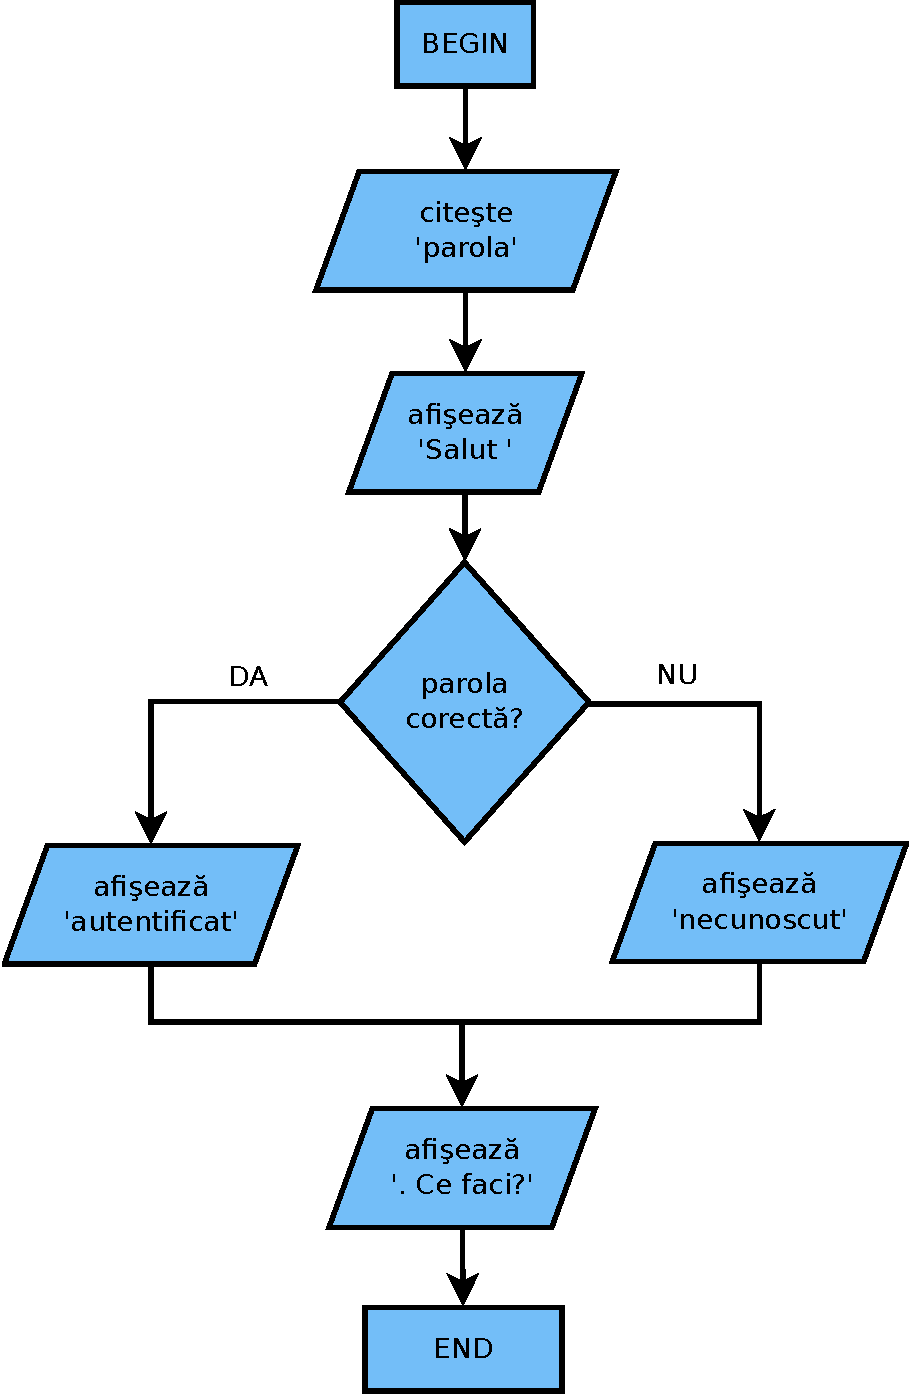
\includegraphics[scale=.5]{cap02/flowchart1-crop.pdf}
  \caption{Flowchart autentificare}
  \label{fig:flowchart authenticated}
\end{figure}

%\needspace{4\baselineskip}
Regula de bază la interpretarea unei scheme logice
este să urmezi în mod stupid săgeţile, la fel ca şi
coiotul nostru din figura \ref{fig:coyote arrow}.

O schemă logică are doar un singur bloc {\glqq}BEGIN{\grqq}, şi unul
sau mai multe blocuri {\glqq}END{\grqq}. O schemă logică curată
ar trebui să aibe totuşi un singur bloc {\glqq}END{\grqq}
către care conduc toate {\glqq}cărările{\grqq} de execuţie posibile.

Operaţiile de input/output sunt puse în paralelograme,
iar operaţiile decizionale sunt puse în romburi şi au
una sau două ieşiri, pentru cazurile {\glqq}DA{\grqq} respectiv {\glqq}NU{\grqq}
în care condiţia este adevărată sau falsă.

\begin{figure}[h!]
  \centering
    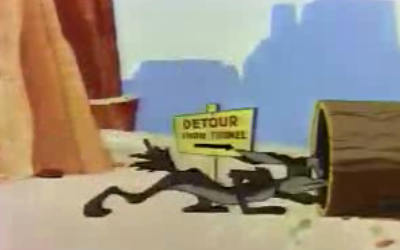
\includegraphics[scale=.8]{cap02/coyote-arrow.png}
  \caption{Cum să urmezi săgeţile}
  \label{fig:coyote arrow}
\end{figure}

Revenim asupra definiţiei fluxului de execuţie, folosindu-ne de scheme logice de data asta:
\textit{fluxul de execuţie} este constituit din săgeţile concrete parcurse de PHP
la executarea scriptului.

\begin{Exercise}[difficulty=2,title={Găseşte eroarea de logică}]
\ExePart
Care sunt greşelile algoritmice din pseudocodul următor?

\begin{lstlisting}[language=pseudocod]
daca parola este corecta
	afiseaza 'autentificat'
altfel
	afiseaza 'parola este gresita'
afiseaza 'aceasta este o informatie secreta '
afiseaza 'vizibila doar utilizatorilor autentificati'
\end{lstlisting}

Identifică-le, explică-le în cuvinte, şi rescrie pseudocodul corect.

Foloseşte-ţi intuiţia pentru a determina ce ar trebui
să facă un astfel de algoritm şi ce nu, pe baza outputului.

\ExePart
Desenează două scheme logice, una pentru pseudocodul (greşit)
din partea I a exerciţiului, şi una pentru varianta corectă
a pseudocodului pe care ai găsit-o ca soluţie în partea I.
\end{Exercise}


\section{Tipul de date boolean. Expresii logice}
\label{sec:tipul de date boolean. Expresii logice}

Secţiunea anterioară a tratat {\glqq}parola este corectă{\grqq} ca ceva
de la sine înţeles. Poate pentru noi este uşor de înţeles,
însă PHP, şi algoritmii în general, nu au noţiunea de {\glqq}corect{\grqq}.

Ce înseamnă {\glqq}corect{\grqq} de fapt? Cum determinăm noi, oamenii,
dacă o adresă, un nume, sau în cazul de faţă o parolă, este corectă?
Ceea ce facem este de fapt compararea a ceva ce vine din exterior, a
unui input, cu ceea ce considerăm noi {\glqq}corect{\grqq}, pe baza cunoştinţelor
sau experienţelor {\glqq}salvate{\grqq} în creierul nostru.\footnote{Procesele
cognitive sunt omise în mod conştient, pentru a simplifica imaginea.}

De exact acest lucru are nevoie şi PHP. Bine ai venit în lumea
expresiilor logice. 

Există nenumăraţi operatori logici. Însă înainte de a trece
la ei, trebuie să introducem o funcţie numită \texttt{var\_dump()}.
În capitolul următor vei învăţa despre funcţii pe larg,
însă deocamdată o mică definiţie: \textit{O funcţie este
ca o {\glqq}cutie neagră{\grqq}. O hrăneşti cu parametri, şi ea face ceva cu
acele valori}. În cazul nostru, vom folosi funcţia \texttt{var\_dump()}
în loc de cuvântul cheie \texttt{echo} pentru a afişa atât valoarea
pe care i-o pasăm ca parametru, cât şi tipul său de date. \texttt{echo}
nu ar fi bun pentru asta deoarece ar face automat nişte conversii
între tipuri de date, şi exact acele tipuri de date sunt ceea ce
vrem să vedem neschimbat.


Toate expresiile logice, care conţin operatori
logici,\footnote{nu neapărat, dar voi vorbi mai târziu
despre asta} sunt evaluate şi au în final
fie valoarea {\glqq}adevărat{\grqq}, fie valoarea {\glqq}fals{\grqq}. Deoarece
expresiile logice sunt atât de importante,\footnote{Există
chiar şi o matematică care le susţine.}
pentru ele există şi un tip de date: \textsl{boolean}, sau pe scurt: bool.
Acesta este al patrulea tip de date cu care faci cunoştinţă, după
string (şir de caractere), int (integer -- număr întreg)
şi float (număr cu virgulă).

În contrast cu celelalte tipuri de date, informaţii de tipul
boolean nu pot avea decât două valori: \texttt{TRUE} sau \texttt{FALSE}.

De exemplu, într-o aplicaţie complexă, în care unii utilizatori
au drepturi speciale, am putea întâlni:
\begin{lstlisting}
$este_administrator = TRUE;
\end{lstlisting}
Însă în loc de \texttt{echo}, vom folosi \texttt{var\_dump()}, în felul următor:
\begin{lstlisting}[firstnumber=2]
var_dump($este_administrator);
\end{lstlisting}
Încearcă, să vezi ce îţi afişează. Bineînţeles că poţi afişa şi valorile
constante \texttt{TRUE} sau \texttt{FALSE} direct:
\begin{lstlisting}
<?php
var_dump(TRUE);
var_dump(FALSE);
\end{lstlisting}

Acum că ştim cum se foloseşte o funcţie precum \texttt{var\_dump()},
hai să revenim la ideea noastră iniţială: PHP nu ştie ce
înseamnă pentru noi {\glqq}parolă corectă{\grqq}, deci trebuie să confruntăm
cele două valori şi să decidem dacă ele sunt una şi aceeaşi.

Aici intră operatorul de comparaţie în joc, \texttt{==}. Acesta
este capabil să compare valorile a două expresii.

\attention{Din lucrul nostru cu \texttt{echo} din secţiunile anterioare,
ştii că o expresie poate fi orice are o valoare, fie ea constantă,
variabilă, rezultatul unei concatenări sau de ce nu, rezultatul
unor operaţii matematice.}

Ne putem da seama cu uşurinţă cum funcţionează următorul cod:
\begin{lstlisting}
<?php
$input = 'asdfgh';//conform unor studii, o parola foarte des folosita

echo '3==4? ';
var_dump(3 == 4);
echo 'foo=foo? ';
var_dump('foo' == 'foo');
echo 'inputul utilizatorului este corect? ';
var_dump($input == 'secret');
echo '3 + -2 = 0? ';
var_dump(3 + -2 == 0);
\end{lstlisting}

Deoarece nu ştim încă cum să cerem input de la utilizator
în adevăratul sens al cuvântului, simulăm asta folosind variabila \texttt{\$input}.
Testează acelaşi cod, schimbându-i valoarea în parola corectă,
să vezi ce se întâmplă. În rest, totul ar trebui să fie evident: comparaţia
este evaluată şi are fie valoarea \texttt{TRUE}, fie valoarea \texttt{FALSE},
care este afişată de \texttt{var\_dump()}.

Următorul exemplu ar trebui să ne pună pe gânduri:
\begin{lstlisting}
<?php
var_dump('42' == 42);
\end{lstlisting}
În interiorul lui PHP, cele două valori, stringul '42'
şi int-ul 42, sunt valori complet diferite. Însă
după cum am spus, PHP face tot posibilul pentru a
converti o valoare de un tip de date într-o \textit{altă}
valoare de alt tip de date, care să reflecte cât mai bine
valoarea iniţială, înainte de conversie.
Din acest motiv, expresia \texttt{'42' == 42} este evaluată
ca \texttt{TRUE}, stringul '42' fiind convertit în int-ul 42 înainte
de evaluarea egalităţii celor două valori constante.

În PHP există însă şi \textsl{operatorul de comparaţie strictă}, cu
verificarea adiţională a tipului de date, folosind operatorul
\texttt{===}.

\begin{Exercise}[title={Verifică-ţi puterea de a face analogii},difficulty=1]
Scrie un cod PHP care să afişeze valorile a patru comparaţii stricte:
\begin{enumerate}
	\item dintre un int şi un string
	\item dintre un float şi un int
	\item dintre un string şi un float
	\item dintre un bool şi un string
\end{enumerate}
\end{Exercise}

\begin{Exercise}[title={Am sintetizat corect noţiunea de \textit{expresie}?},difficulty=2]
\ExePart
Scrie un cod PHP care să afişeze valoarea booleană a unei comparaţii
stricte dintre o expresie matematică şi un string.

Expresia matematică trebuie să conţină cel puţin o operaţie de gradul I, una
de gradul II, şi să folosească cel puţin o dată parantezele rotunde pentru
grupare.
\ExePart

Explică în cuvinte ce face următorul cod:

\begin{lstlisting}
<?php
$foo = 4 == '5';
\end{lstlisting}
\attention{Dacă ai dificultăţi la rezolvarea exerciţiului, ar trebui să reciteşti încă o dată
totul cu atenţie, începând de la pagina \pageref{sec:output simplu}.
}
\end{Exercise}

Operatorii logici de comparaţie şi de comparaţie strictă se mai numesc
şi \textsl{operatori relaţionali}, deoarece valoarea de adevăr rezultată
în urma comparaţiei stabileşte relaţia dintre cei doi operanzi.

Operaţiile logice de verificare a egalităţii şi de verificare strictă
a egalităţii pot fi negate. Acest lucru se face înlocuind primul '='
al fiecărui operator cu simbolul '!'. Astfel '!=' se citeşte \textit{este diferit de},
iar '!==' se citeşte \textit{este strict diferit de}.

Pe lângă relaţia de egalitate, mai există şi operatori logici relaţionali
care stabilesc inegalitatea. Aceştia sunt ilustraţi în
tabelul \ref{tbl:operatori inegalitate}.

\begin{table}[h!]
  \begin{center}
  	  \begin{tabular}{| c | l |}
	  \hline
	  Operator & Semnificaţie \\
	  \hline
	  \texttt{<}	& mai mic \\
	  \texttt{>}	& mai mare \\
	  \texttt{<=}	& mai mic sau egal \\
	  \texttt{>=}	& mai mare sau egal \\
	  \hline
	  \end{tabular}
  \end{center}
  \caption{Operatorii de inegalitate}
  \label{tbl:operatori inegalitate}
\end{table}


\subsection{Conjuncţii, disjuncţii şi negaţii}
În paginile anterioare ai făcut cunoştinţă cu expresii logice
simple. Este însă posibil să unim mai multe expresii booleene,
iar ceea ce rezultă este la final tot o expresie logică booleană,
deci va avea una din valorile TRUE sau FALSE.

Aceste operaţii se numesc conjuncţii şi disjuncţii.

O \textsl{disjuncţie}
reprezintă o alternativă. Colocvial recunoaştem disjuncţiile
după cuvântul \textit{sau}. În practică, am putea spune
\textit{Dacă plouă sau ninge, atunci îmi iau ghetele}. Nu contează
care dintre evenimente va avea loc (sau în termeni booleeni: \textit{care dintre
evenimente {\glqq}vor fi adevărate{\grqq}}), unul sau chiar ambele, disjuncţia
va fi în orice caz adevărată.

Având două expresii booleene A şi B, fiecare cu una din valorile de
adevăr T (TRUE) sau F (FALSE), în formalism matematic am face calcule de genul:

\[ 
  \left.
  \begin{array}{c}
    A = T\\
    B = F
  \end{array}
  \right\}
  \Rightarrow A \lor B = T \lor F = T
\]

O \textsl{conjuncţie} în schimb este adevărată doar dacă ambele expresii logice A şi B
sunt adevărate. În limbajul de zi cu zi recunoaştem conjuncţiile după cuvântul \textit{şi}.

Formalismul matematic pentru aceeaşi situaţie ca mai sus ar arăta astfel:

\[ 
  \left.
  \begin{array}{c}
    A = T\\
    B = F
  \end{array}
  \right\}
  \Rightarrow A \land B = T \land F = F
\]

Simbolurile matematice pentru disjuncţii şi conjuncţii sunt $\lor$ respectiv $\land$, şi se citesc
{\glqq}sau{\grqq} respectiv {\glqq}şi{\grqq}. În PHP, aceste operaţii sunt făcute de operatorii {\glqq}||{\grqq}, respectiv {\glqq}\&\&{\grqq}.

Pentru toate combinaţiile de TRUE şi FALSE,
\engl{tabelul de adevăr\footnote{\url{http://en.wikipedia.org/wiki/Truth_table}}}{truth table} pentru
cele două operaţii este ilustrat în tabelul \ref{tbl:truth table and or}.



După cum observi, conjuncţiile şi disjuncţiile sunt comutative -- ceea ce înseamnă
că ordinea lor nu contează, rezultatul va fi acelaşi. Acest lucru este adevărat,
matematic vorbind, însă există unele cazuri în care, în programare, există totuşi
diferenţe. Ne vom uita la aceste diferenţe peste câteva secţiuni.

Pe lângă conjuncţii şi disjuncţii, mai putem şi nega o expresie logică. Pentru
asta folosim operatorul '!' (în PHP), citit \textit{not}. Simbolul matematic
este $\lnot$. $\lnot$TRUE este deci FALSE, iar $\lnot$FALSE este TRUE, sau în cuvinte:
\textit{negarea unei afirmaţii este o negaţie}, respectiv \textit{negarea unei negaţii este o afirmaţie}.

Deoarece în urma unei operaţii logice ne alegem tot cu o valoare booleană,
putem înlănţui două sau mai multe operaţii logice, unindu-le printr-o operaţie logică.
Bineînţeles că putem şi grupa operaţii logice cu paranteze rotunde, la fel
ca operaţiile matematice.

De exemplu, 
$\lnot(T \land F) \lor T$ va fi mereu TRUE, deoarece, oricare ar fi rezultatul negaţiei
expresiei din paranteză,
avem apoi o disjuncţie, iar \textit{<orice> SAU TRUE} este mereu TRUE.


\begin{Exercise}[title={Legile lui De Morgan},difficulty=2]
Cei inteligenţi dintre noi au realizat deja că \textit{negarea unei conjuncţii este echivalentă
cu disjuncţia negaţiei fiecăruia dintre cei doi operanzi}, şi vice-versa: \textit{negarea unei disjuncţii
este echivalentă cu conjuncţia negaţiei fiecăruia dintre cei doi operanzi}.

Fă un tabel de adevăr similar cu tabelul \ref{tbl:truth table and or}, în care calculezi
valorile echivalentelor expresiilor $\lnot(A \lor B)$ respectiv $\lnot(A \land B)$,
echivalente pe care le găseşti aplicând legile lui De Morgan enunţate mai sus.
\end{Exercise}

\begin{Exercise}[title={Operaţii logice},difficulty=1]
Calculează valorile de adevăr a următoarelor expresii:
\begin{enumerate}
  \item $T \land {\lnot}F $
  \item $\lnot(T \lor F) \land T $
  \item $T \land A \lor \lnot(T \land B)$ pentru toate valorile posibile ale lui A şi B. Crează tabelul adevărului cu 5 coloane: A, B, $T \land A$, $\lnot(T \land B)$, şi $T \land A \lor \lnot(T \land B)$
\end{enumerate}
\end{Exercise}

Până acum ne-am pus la punct cunoştinţele teoretice despre algoritmică şi logică. În secţiunile următoare
ne vom uita la utilizarea lor practică în PHP.

\attention{Asigură-te că ai înţeles şi că stâpâneşti toată teoria şi terminologia
prezentate până acum. Lecţiile
următoare \textit{nu} vor mai relua nici una dintre noţiuni, ci vor
trece foarte rapid în revistă sintaxa şi semantica lucrurilor deja învăţate.}


\label{endsec:tipul de date boolean. Expresii logice}

\section{Condiţii -- if şi switch}
În PHP, poţi instrucţiona parserul să execute nişte instrucţiuni doar dacă
o condiţie este adevărată folosind constructul \texttt{if}. După \texttt{if}
urmează, în paranteze rotunde, o expresie logică. Aceasta poate fi orice fel
de expresie booleană, de la simplă la complexă, cu disjuncţii, cojuncţii, negaţii sau
paranteze, exact aşa cum ai văzut în lecţia trecută. După expresia logică urmează un bloc
de instrucţiuni constituit din una sau mai multe instrucţiuni între acolade.

Câteva exemple:
\begin{lstlisting}
<?php
$este_administrator = TRUE;
echo 'Salut';
if(TRUE === $este_administrator) {
  echo ' Administratorule';
}
echo '. Eu voi fi vazut de toata lumea';
\end{lstlisting}
Încearcă acest cod. Apoi schimbă valoarea cu care este iniţializată
variabila \$este\_administrator în FALSE. Ce observi?

\begin{lstlisting}[caption={Utilitatea verificărilor}, label=lst:check_utilisation]
<?php
$este_administrator = TRUE;
echo 'Salut ';
if(TRUE === $este_administrator) {
  echo 'Administratorule';
}
else {
  echo 'Utilizatorule';
}
echo '. Eu voi fi vazut de toata lumea';
\end{lstlisting}
\attention{
În funcţie de valoarea de adevăr a condiţiei (care este o expresie logică),
se execută fie ramura if, fie ramura else. După aceea este continuată execuţia
liniară. Iar ramura \texttt{else} este complet opţională.
}

Felul în care poate fi folosit constructul \texttt{if} este acelaşi cu felul în
care ai folosit {\glqq}constructul{\grqq} \texttt{dacă} în pseudocod şi romburile pentru
decizii în scheme logice. Liniile 2, 3 şi 10 fac parte din execuţia liniară,
linia 4 din ambele exemple crează bifurcaţia 'DA' în fluxul de execuţie,
iar linia 7 crează bifurcaţia 'NU' în al doilea exemplu.

\good{Fi atent la cum am aliniat instrucţiunile, constructele şi acoladele.
Se numeşte formatarea codului, şi este bine să îţi scrii codul formatat
astfel încât doar din alinierea constructelor, ochiul să poată
{\glqq}scana{\grqq} şi decide cât mai uşor cărei ramuri sau bloc aparţine
fiecare instrucţiune, fără a fi nevoit să citeşti cu atenţie
fiecare LOC.}

Aceste constructe decizionale pot fi puse unul în altul (en. \textsl{nested}),
formând algoritmi şi mai complecşi. De exemplu, să ne imaginăm cum
ar arăta codul unei aplicaţii în care vizitatorii pot fi autentificaţi
sau nu, iar unii din utilizatorii autentificaţi au drepturi speciale:
\begin{lstlisting}[caption={Autentificare}, label=lst:authentication]
<?php
$este_autentificat = TRUE;
$este_administrator = TRUE;
if($este_autentificat) {
  echo 'Esti autentificat.';
  if($este_administrator) {
	  echo 'Esti administrator.';
  }
  else {
	  echo 'Nu esti administrator.';
  }
}
else {
  echo 'Nu esti autentificat';
}
\end{lstlisting}

\begin{Exercise}[title={Întrebare de inteligenţă},difficulty=1]
De ce codul anterior nu are în ramura else de pe linia 13 încă
un if/else în interior pentru cazul în care vizitatorul este
şi administrator?
\end{Exercise}


\begin{Exercise}[title={Schemă logică pornind de la cod PHP},difficulty=1]
Desenează schemele logice ale listingurilor 
\ref{lst:check_utilisation} şi \ref{lst:authentication}.
\end{Exercise}

În exemplele anterioare, o variabilă putea satisface o condiţie, sau nu.
Pentru aceste două cazuri am pus instrucţiunile necesare fie în blocul
{\glqq}if{\grqq}, fie în blocul {\glqq}else{\grqq}.
Există însă cazuri în care o variabilă poate lua o valoare dintr-o colecţie de
două sau mai multe valori, şi vrem ca în fiecare caz să fie
executate anumite instrucţiuni. Să zicem că aplicaţia noastră
va avea utilizatori autentificaţi, moderatori şi administratori.
Vom vrea ca toate verificările să nu fie nested, ci liniare:
\begin{lstlisting}
<?php
$rol = 'administrator';
if('autentificat' === $rol) {
  echo 'esti autentificat';
}
else if('moderator' === $rol) {
  echo 'esti moderator';
}
else if('administrator' === $rol) {
  echo 'esti administrator';
}
\end{lstlisting}
Încearcă acest cod de mai multe ori, modificând de fiecare dată valorile
variabilelor, să vezi pe unde trece fluxul de execuţie.

PHP pune la dispoziţie încă un construct pentru astfel de cazuri: \texttt{elseif}.
El este contracţia unei combinaţii \texttt{else if}, ca în exemplul de mai sus.

\begin{Exercise}[title={elseif}]
Rescrie exemplul anterior folosind \texttt{elseif} în loc de \texttt{else if}.
\end{Exercise}

Totuşi, atunci când numărul de posibile valori creşte (să zicem, \$rol poate avea
una din 20 de valori), iar aplicaţia trebuie să le trateze pe fiecare individual,
chiar şi codul cu \texttt{elseif} devine greu de citit.

Pentru astfel de cazuri PHP ne pune la dispoziţie constructul \texttt{switch}.
Sintaxa generală arată astfel:
\begin{lstlisting}
switch($variabila) {
  //aici tratam diferite cazuri
}
\end{lstlisting}
Pentru fiecare valoare posibilă, în interiorul lui \texttt{switch}
punem constructul \texttt{case} urmat de valoarea cu care confruntăm
variabila, si apoi ':'. Vom rescrie exemplul anterior:

\begin{lstlisting}
<?php
$rol = 'administrator';
switch($rol) {
  case 'autentificat':
	  echo 'esti autentificat.';
  case 'moderator':
	  echo 'esti moderator.';
  case 'administrator':
	  echo 'esti administrator.';
}
\end{lstlisting}
Schimbă pe rând valoarea variabilei \texttt{\$rol}. Vei observa că
fluxul de execuţie va potrivi o valoare (liniile 4, 6 sau 8), însă
fluxul de execuţie nu se va opri la blocul {\glqq}case{\grqq} la care a început,
ci se va {\glqq}prelinge{\grqq} mai departe. Pentru a opri, împiedica fluxul de
execuţie să se extindă către celelalte blocuri {\glqq}case{\grqq}, trebuie să
adaugi instrucţiunea \texttt{break}. De exemplu:
\begin{lstlisting}
<?php
$rol = 'administrator';
switch($rol) {
  case 'autentificat':
	  echo 'esti autentificat.';
	  break;
  case 'moderator':
	  echo 'esti moderator.';
  case 'administrator':
	  echo 'esti administrator.';
}
echo 'sunt in afara switch-ului';
\end{lstlisting}
În acest caz, fluxul de execuţie va trece prin linia 10, doar dacă
condiţiile de pe liniile 7 sau 9 sunt îndeplinite. Constructul
\texttt{break} de pe linia 6 va rupe fluxul normal de execuţie,
forţându-l să revină la stadiul liniar de dinainte de switch,
deci continuând execuţia (liniară) cu linia 12.

În cazul în care vrem să tratăm orice altă
valoare netratată de niciun bloc \texttt{case}, putem
folosi ramificaţia \texttt{default}, astfel:

\begin{lstlisting}
<?php
$rol = 'administrator';
switch($rol) {
  case 'autentificat':
	  echo 'esti autentificat.';
	  break;
  case 'moderator':
	  echo 'esti moderator.';
	  break;
  case 'administrator':
	  echo 'esti administrator.';
	  break;
  default:
	  echo 'rolul tau este invalid';
}
echo 'sunt in afara switch-ului';
\end{lstlisting}
Ramura \texttt{default} nu mai are nevoie de \texttt{break} deoarece
este ultima ramură din blocul switch.

\attention{Ultima ramură din \texttt{switch}, fie ea \texttt{case} sau \texttt{default},
nu are nevoie de \texttt{break}, deoarece nu mai există nicio altă
ramură după, deci fluxul de execuţie nu riscă să
intre pe o ramură nedorită.}

În unele cazuri, vom vrea să-i atribuim unei variabile o valoare
pe baza unei condiţii. Pentru astfel de cazuri există încă un
operator, numit \textsl{operatorul ternar}. Se numeşte astfel deoarece
este singurul operator cu trei operanzi.

Sintaxa generală este:
\begin{verbatim}
<condiţie> ? <dacă-TRUE> : <dacă-FALSE>;
\end{verbatim}
Acest întreg {\glqq}conglomerat{\grqq} va fi înlocuit de
una din expresiile <dacă-TRUE> sau <dacă-FALSE>,
în funcţie de valoarea de adevăr a condiţiei.

\attention{Asta înseamnă că întregul construct
poate fi {\glqq}pus{\grqq} oriunde PHP acceptă o expresie.
Deoarece <dacă-TRUE> şi <dacă-FALSE> sunt ele înseşi
expresii, putem avea deci operaţii ternare una în alta
(en. \textit{nested}).}

Ceea ce am fi scris anterior astfel:
\begin{lstlisting}
<?php
$rol = 'administrator';
if('administrator === $rol) {
  $este_administrator = TRUE;
}
else {
  $este_administrator = FALSE;
}
var_dump($este_administrator);
\end{lstlisting}
putem scrie mult mai compact astfel:
\begin{lstlisting}
<?php
$rol = 'administrator';
$este_administrator = 'administrator' === $rol ? TRUE : FALSE;
var_dump($este_administrator);
\end{lstlisting}
\begin{Exercise}[title={Înţelegerea operatorului ternar},difficulty=2]
\ExePart
Explică în cuvinte ce face linia 3 din exemplul anterior.

\ExePart
Explică în cuvinte ce se întâmplă concret în acest cod:
\begin{lstlisting}
<?php
$rol = 'administrator';
if('test' === ($rol === 'administrator' ? 'test' : 'test2')) {
        echo 'administrator';
}
\end{lstlisting}
Pentru două cazuri, când \$rol are valoarea 'administrator', şi când
are o altă valoare.
\end{Exercise}

\section{Buclele while şi do while}
Buclele constituie modalitatea de a executa un bloc de instrucţiuni
în mod repetitiv, atâta timp cât o condiţie este adevărată.

Sintactic, cele două bucle, \texttt{while} şi \texttt{do while} arată astfel:
\begin{lstlisting}
while(<conditie>) {
  <bloc-de-instructiuni>
}
do {
  <bloc-de-instructiuni>
} while(<conditie>);
\end{lstlisting}

Schema logică a buclei while arată ca în figura \ref{fig:flowchart while loop}.

\begin{figure}[h!]
  \centering
    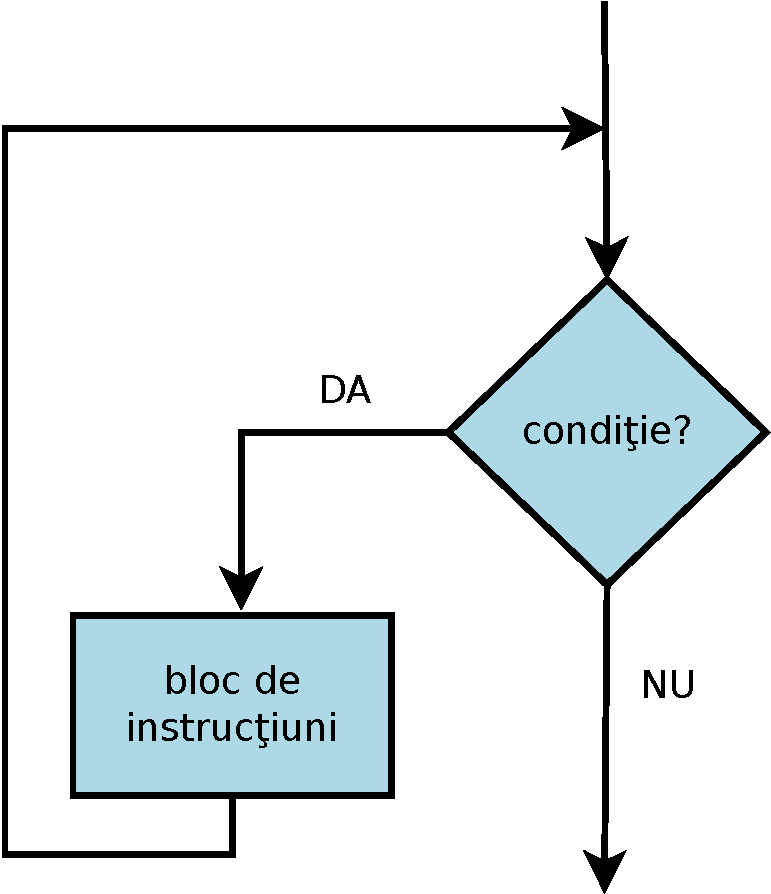
\includegraphics[scale=.5]{cap02/while-crop.pdf}
  \caption{Flowchart buclă while}
  \label{fig:flowchart while loop}
\end{figure}

Dacă condiţia este din start falsă, atunci se continuă execuţia liniară ({\glqq}în jos{\grqq}),
altfel se trece prin blocul de instrucţiuni (care bineînţeles că poate
conţine mai multe instrucţiuni, sau chiar alte bucle, constructe if/else, switch, ş.a.m.d.).
După ce instrucţiunile au fost executate, se ajunge iar la verificarea condiţiei,
şi povestea o poate lua de la capăt.

\attention{Blocul de instrucţiuni trebuie să modifice cumva valoarea de adevăr
a condiţiei care urmează a fi verificate. Altfel riscăm să creăm o buclă
infinită, din care fluxul de execuţie nu va ieşi niciodată.

La acest lucru se ajunge de obicei folosind cel puţin o variabilă în condiţie,
a cărei valoare se schimbă în blocul de instrucţiuni.}

De exemplu, putem număra de la unu la zece, din unu în unu. Pentru asta,
valoarea de start este evident 1. Această valoare o vom salva într-o variabilă.
La fiecare rulare a buclei, adunăm 1 la valoarea variabilei, şi salvăm
rezultatul în aceeaşi variabilă. Astfel avansăm de la 1 la 2, de la 2 la 3,
ş.a.m.d., până la 10. Condiţia de oprire va fi ca valoarea variabilei să
fie mai mică sau egală cu 10. Dacă condiţia nu este adevărată, atunci fluxul de execuţie
{\glqq}trece peste{\grqq} blocul while, şi se continuă execuţia liniară.

Schema logică ar arăta ca în figura \ref{fig:while counting}.

\begin{figure}[h!]
  \centering
    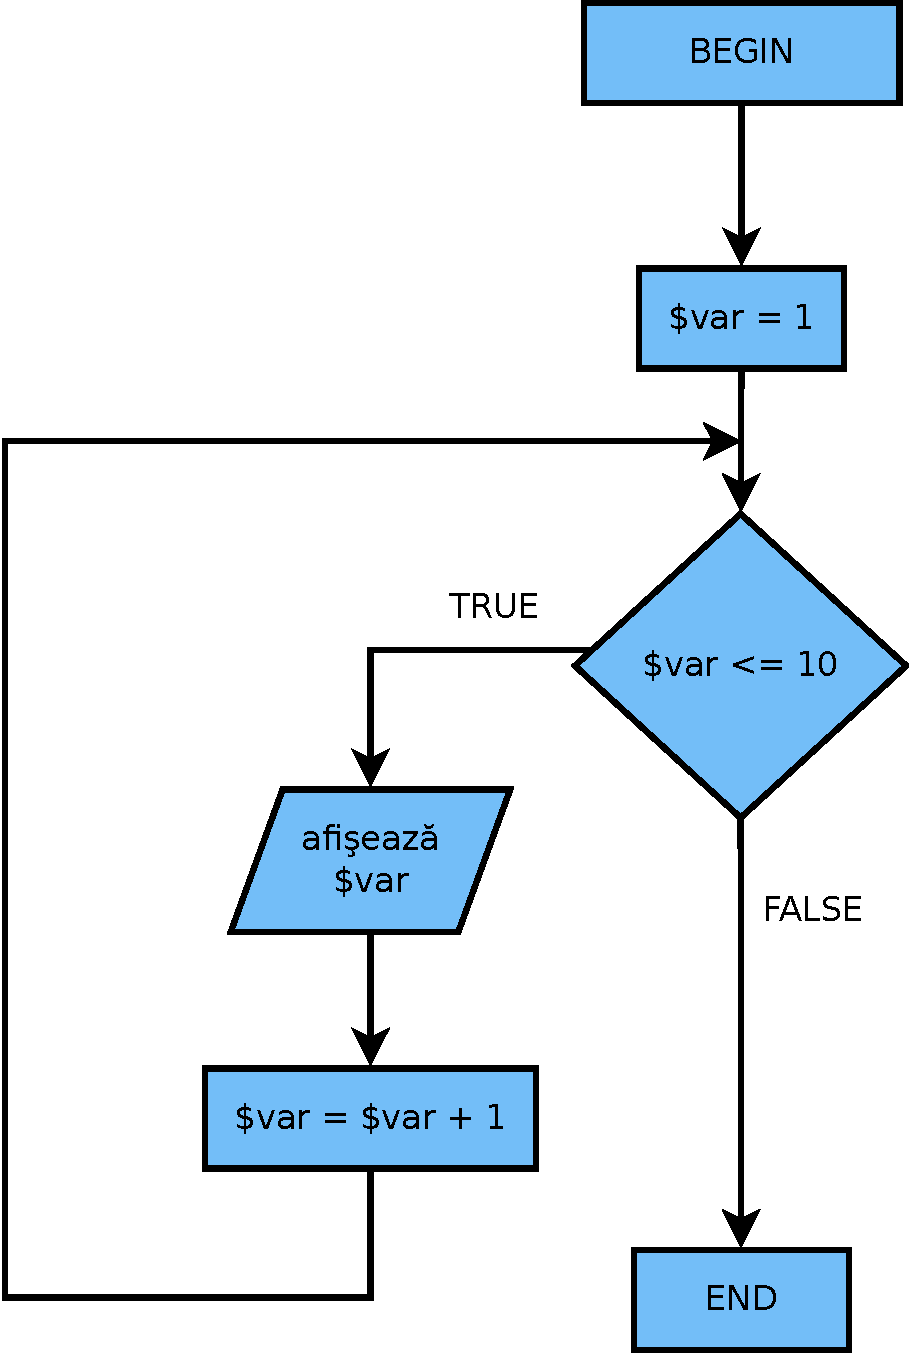
\includegraphics[scale=.5]{cap02/count-while-crop.pdf}
  \caption{Numărând de la 1 la 10}
  \label{fig:while counting}
\end{figure}

\begin{Exercise}[title={Numărătoarea din 1 în 1 cu while},difficulty=1]
\ExePart
Implementează algoritmul din figura \ref{fig:while counting} în limbajul PHP.

\ExePart
Întrebare capcană: Ce valori va lua pe rând variabila \$var?
\end{Exercise}

\texttt{Do while} este foarte asemănătoare cu bucla \texttt{while},
diferenţa fiind că blocul de instrucţiuni va fi executat cel
puţin o dată. Ceea ce este logic, din moment ce mai întâi se
trece prin blocul de instrucţiuni, apoi este verificată condiţia, şi
dacă aceasta este TRUE, atunci se sare înapoi, la începutul blocului de
instrucţiuni.

În altă ordine de idei, iniţial blocul de instrucţiuni
face parte din execuţia liniară. Abia apoi se va decide, în funcţie de valoarea
de adevăr a condiţiei, dacă se va crea o buclă sau nu. Din asta deducem
că fluxul de execuţie poate trece prin {\glqq}bucla{\grqq} \texttt{do while} fără
a face nicio buclă de fapt, fără a sări înapoi nici măcar o dată. Asta s-ar putea
întâmpla dacă condiţia ar fi din start falsă. Însă în contrast cu bucla
\texttt{while}, blocul de instrucţiuni al buclei \texttt{do while} va fi executat cel
puţin o dată.

\begin{Exercise}[title={Schema logică a buclei do while},difficulty=1]
Modifică schema logică generală a buclei \texttt{while} din
figura \ref{fig:flowchart while loop}, transformând-o în
schema logică a buclei \texttt{do while}.
\end{Exercise}


\begin{Exercise}[title={Numărătoarea din doi în doi cu do while},difficulty=1]
\ExePart
Scrie un program care să numere descrescător din 2 în 2, începând de la 23
şi terminând cu un număr negativ la alegere, folosind bucla do while.

\ExePart
Ce face programul tău şi nu este în cerinţă?
\end{Exercise}

\begin{Exercise}[title={Par sau impar?},difficulty=2]
Alege un număr pozitiv nenul N şi scrie un program care
pentru toate numerele din intervalul [-N;N] afişează dacă acestea sunt pare
sau impare. Pentru N=42, outputul va arăta astfel:
\begin{verbatim}
-42 este par
-41 este impar
-40 este par
...
0 este par
...
41 este impar
42 este par
\end{verbatim}
Valorile constante 'este', 'par' şi 'impar' trebuie să apară o singură dată în
cod, iar codul trebuie să facă uz de operatorul ternar şi de operatorul modulo.
\end{Exercise}

\subsection{break şi continue}
Constructul \texttt{break} l-am întâlnit deja în folosirea constructului
\texttt{switch}. Însă \texttt{break}, după cum îi sugerează şi numele, poate
mai mult: poate întrerupe orice buclă.\footnote{A nu se înţelege că \texttt{switch} ar fi o buclă -- nu este}
Fluxul de execuţie din buclă pur şi simplu
va sări din interiorul buclei în afara ei, continuând fluxul liniar
de după buclă.

Unul din scenariile în care avem nevoie de el ar putea fi căutarea:
căutăm un element într-o buclă, şi atunci când l-am găsit, întrerupem
căutarea -- nu ar mai avea rost să terminăm de iterat tot setul de date.

De exemplu, dându-se un număr întreg N ca input, vrem să aflăm următorul
multiplu de 10. Am putea face asta în felul următor:

\begin{lstlisting}
<?php
$n = 231;

while(TRUE === TRUE) {
  if(0 === $n%10) {
	  break;
  }
  $n += 1;
}

echo 'N rotunjit prin adaugire este ',$n;
\end{lstlisting}

Linia 4 ne-ar putea părea ciudată, şi într-adevăr este.
Ea transformă automat bucla while într-una infinită,
deoarece, în mod evident, valoarea de adevăr a comparaţiei nu se va schimba
niciodată. Însă acest lucru este voit, deoarece practic întrerupem
bucla fluxului de execuţie folosind break.

\attention{Dacă nu înţelegi
linia 5, atunci cel mai probabil nu ai sintetizat destul
la ce este util restul operaţiei de împărţire, şi deci
operatorul modulo, prezentat la pagina \pageref{term:modulo}.}

\good{Revizuieşte lecţia \textit{Teorema împărţirii cu rest},
învăţată la matematică în clasa a V-a.}

\begin{Exercise}[title={Majoritatea buclelor infinite pot fi corectate}]
Rescrie codul anterior mutând (şi eventual modificând) condiţia
de întrerupere a buclei (deci condiţia din \texttt{if}),
şi renunţând complet la folosirea \texttt{break}.

Ce crezi, codul este acum mai curat sau nu?
\end{Exercise}

Constructul \texttt{continue} ne permite să
sărim peste restul instrucţiunilor următoare
din ciclul curent al buclei, trecând la ciclul următor.

De exemplu, putem afişa doar numerele care sunt multiple
de trei, şi calcula suma celorlalte numere din intervalul
de numere [0,50] astfel:
\begin{lstlisting}
<?php
$n = 0;
$sum = 0;
while($n <= 50) {
  if(0 === $n%3) {
	  echo $n,' ';
	  $n += 1;
	  continue;
  }
  $sum += $n;
  $n += 1;
}
echo 'Suma este ',$sum;
\end{lstlisting}
Datorită liniei 8, fluxul de execuţie va sări înapoi pe linia 4.
Deoarece la următoarea iteraţie a buclei nu vrem să intrăm cu aceeaşi valoare pentru \$n,
căci ne-am alege cu o buclă infinită, adăugăm 1 la valoarea lui \$n, şi
salvăm rezultatul tot în \$n pe linia 7, înainte de a face saltul înapoi la verificarea
condiţiei.
 

\section{Tipul de date array. Bucla foreach}
Până acum am lucrat doar cu \textsl{tipuri de date scalare}: string, int, float, bool.
Un array este un tip de date \textsl{compozit} şi poate fi folosit în cele mai
diverse situaţii, motiv pentru care este foarte versatil.

Pentru a iniţializa un array, atribuim valoarea \texttt{array()} unei variabile.
Aceasta va conţine un array gol. Exemplu:
\begin{lstlisting}
<?php
$a = array();
var_dump($a);
var_dump(array());
\end{lstlisting}
Din asta deducem că \texttt{array()} poate fi la fel de bine o expresie,
deci poate fi folosit aşa cum am folosit orice altă valoare de până acum,
precum TRUE, 42, sau 'foo':
\begin{lstlisting}
<?php
$a = array();
var_dump($a === array());
if($a === array()) {
  echo '$a este un array gol';
}
\end{lstlisting}

În loc de a compara o variabilă cu \texttt{array()}, PHP
ne pune la dispoziţie un construct special: \texttt{empty()}.
Acesta, împreună cu variabila din interiorul parantezelor
rotunde, este înlocuit de o valoare booleană. Testează
următorul exemplu:
\begin{lstlisting}
<?php
$a = array();
var_dump(empty($a));
\end{lstlisting}
Concluzionăm că \texttt{empty()} poate fi folosit oriunde
am folosit până acum expresii logice, de exemplu în if:

\begin{lstlisting}
<?php
$a = array();
if(TRUE === empty($a)) {
  echo '$a este gol';
}
else {
  echo '$a este plin';
}
\end{lstlisting}

Pentru a iniţializa un array cu elemente în el, le putem
pune între parantezele rotunde ale lui \texttt{array()},
separându-le unul de altul prin virgulă:
\begin{lstlisting}
<?php
$a = array(42,'foo',TRUE,FALSE);
if(TRUE === empty($a)) {
  echo '$a este gol';
}
else {
  echo '$a este plin';
}
\end{lstlisting}
Sper că acum este evident de ce un array este un tip de
date compozit: în el poţi salva alte valori de diferite tipuri
de date.

Exact, un array salvează în el valori precum cele constante
de mai sus. Putem chiar şi copia valorile altor variabile
în array:
\begin{lstlisting}
<?php
$foo = 'bar';
$a = array(42,$foo);
\end{lstlisting}
\attention{Este incorect să spui că variabila \texttt{\$foo} este în array-ul \texttt{\$a}. Nu
variabila este într-un array, ci valoarea acesteia. A doua linie se citeşte deci
astfel: \textit{Copiază valoarea constantă 42 şi valoarea variabilei \texttt{\$foo} într-un array,
şi atribuie array-ul rezultat variabilei \$a}.}

După ce avem un array, vom vrea să prelucrăm valorile
salvate în el într-o buclă, fiecare element pe rând.

Deoarece array-urile sunt foarte importante, PHP
ne pune la dispoziţie încă o buclă, special gândită
pentru ceea ce numim \textsl{iterarea array-urilor}.
Bucla se numeşte \texttt{foreach}.

Sintaxa generală arată astfel:
\begin{verbatim}
foreach(<array>  'as' <value>) {
  <bloc-de-instructiuni>
}
\end{verbatim}
<array> este array-ul pe care vrem să-l iterăm, <value>
este o variabilă inventată de noi care există
doar în interiorul buclei şi care va lua pe rând
valorile păstrate în array, la fiecare iteraţie a buclei.

Să zicem că avem o listă de nume, şi vrem să le afişăm pe toate
unul sub altul, în HTML:
\begin{lstlisting}
<?php
$names = array('Mircea','Claudiu','Ioana','Flavius');

foreach($names as $name) {
  echo 'Salut ', $name,'!<br>';
}
echo 'Hooray!';
\end{lstlisting}

\begin{Exercise}[title={Meniu de navigare},difficulty=1]

\ExePart

Scrie un cod care pornind de la un array precum
\begin{lstlisting}
$menu = array('Home','Contact','Despre');
\end{lstlisting}
generează un meniu de navigare (tag-urile \texttt{<ul>} şi \texttt{<li>}).
Structura codului HTML va trebui să arate astfel:
\begin{verbatim}
<ul>
        <li><a href="#Home">Home</a></li>
        <li><a href="#Contact">Contact</a></li>
        <li><a href="#Despre">Despre</a></li>
</ul>
\end{verbatim}

\ExePart
Îmbunătăţeşte codul astfel încât dacă \texttt{\$menu} este iniţializat gol, astfel:
\begin{lstlisting}
$menu = array();
\end{lstlisting}
să nu mai genereze un meniu, ci output-ul:
\begin{verbatim}
Meniu inexistent.
\end{verbatim}
Pentru asta va trebui să verifici dacă array-ul este gol cu \texttt{empty(\$menu)}, dacă
nu, să faci ceea ce ai făcut în partea I a exerciţiului, altfel să generezi
outputul 'Meniu inexistent'.
\end{Exercise}
Exerciţiul \textit{Meniu de navigare} ţi-a introdus subtil avantajele
array-urilor. Este adevărat că la început codul va fi mult mai
complex decât un meniu static în HTML, însă după ce ai codul, şi
acesta funcţionează, nu trebuie decât să modifici valorile salvate
în array, într-un loc {\glqq}central{\grqq}, şi PHP va genera mereu meniul HTML corespunzător.
Nu vei mai avea de-a face cu HTML direct, nu mai mult decât ai descrie un singur element
\texttt{<li>}, un singur element \texttt{<ul>} sau un singur element \texttt{<a>}.
Asta este posibil mulţumită proprietăţii unei bucle de a repeta un bloc de instrucţiuni.

Ceea ce am făcut în exerciţiul anterior
se numeşte \textit{inventarea unei structuri de date abstracte} (în cazul
nostru este un array, pe care
l-am salvat în \texttt{\$menu}) care emulează ceea ce cunoaştem ca fiind un {\glqq}meniu{\grqq} în {\glqq}viaţa reală{\grqq}.
Deşi nu este el însuşi un meniu, conţine toate datele de care avem nevoie
pentru a genera dinamic un meniu, cu PHP. Aceste date se numesc \textsl{metadate},
concept pe care l-ai cunoscut la începutul acestui capitol.

\attention{După cum ţi-am spus încă de la începutul capitolului, şi după
cum tocmai ai văzut, toate aplicaţiile conţin metadate. Ele vin
deseori {\glqq}împachetate{\grqq} în structuri de date abstracte precum array-ul
salvat în \texttt{\$menu}.}
\good{Obişnuieşte-te cu ideea de a trebui să inventezi date abstracte
care conţin metadate.
%Prin introducerea acestor date abstracte codul tău va fi mai flexibil şi mai mentenabil.
Este adevărat,
la început va trebui să investeşti mai mult timp în
conceperea acestor date abstracte, dar pe termen lung avantajele
în termeni de \textit{mentenabilitate}, \textit{flexibilitate} şi \textit{reutilizare}
a codului se vor face simţite.}

După ce un array a fost iniţializat, putem adăuga elemente adiţionale
la sfârşitul său, folosind operatorul \texttt{[]}. Sintaxa generală este:
\begin{verbatim}
$<array>'[]' = <valoare>
\end{verbatim}
Exemplu:
\begin{lstlisting}[label=lst:push_operator,caption={Adăugarea elementelor la sfârşitul unui array}]
<?php
$names = array('Mircea','Claudiu','Ioana','Flavius');
$names[] = 'Ramona';
\end{lstlisting}
Convinge-te, scrie un cod care iterează array-ul rezultat după adăugarea
elementului 'Ramona'.

Până acum, la fiecare iteraţie a array-ului, valoarea curentă era
pusă în variabila de după \texttt{as}. Însă elementele dintr-un array
au şi un index, o ordine. Pentru a ajunge la acest index, \texttt{foreach}
are o sintaxă extinsă:
\begin{verbatim}
foreach(<array> 'as' <index> '=>' <valoare>) {
  <bloc-de-instructiuni>
}
\end{verbatim}

\begin{Exercise}[title={Sintaxa foreach},difficulty=2]
Scrie un program care iterează toate elementele dintr-un array
şi afişează pentru fiecare 'Elementul <I> are valoarea <V>', unde <I>
este indexul, <V> este valoarea.

\attention{Acest exerciţiu îţi testează capacitatea de a înţelege
o specificaţie sintactică şi de a o aplica în practică,
scriind un cod PHP care o respectă.}
\end{Exercise}

După cum ai observat, elementele dintr-un array sunt numerotate
de la zero la N-1, unde N este numărul total de elemente. Din acest motiv,
spunem că un array este \textsl{0-indexed}. Astfel de array-uri se
mai numesc şi \textsl{vectori} sau \textsl{liste}.

Pot exista situaţii în care vrem un anumit element din array, ştiindu-i
indexul. În astfel de cazuri folosim sintaxa următoare pentru a accesa
acel element:
\begin{verbatim}
$<array>'['<index>']'
\end{verbatim}
<index> poate fi orice expresie care are o valore, aşa cum am văzut până acum,
deci asta include şi operaţii matematice:
\begin{lstlisting}
<?php
$names = array('Mircea','Claudiu','Ioana','Flavius');

$index_fata = 2;

echo 'Eu sunt ',$names[3],'<br>';
echo 'Pe fata o cheama ',$names[$index_fata],', inaintea ei este ',
		  $names[$index_fata-1],' iar dupa ea urmeaza ',$names[$index_fata+1];
\end{lstlisting}

Să zicem că avem următoarea situaţie: avem un array de nume,
şi numele nostru şi vrem să afişăm numele imediat după numele nostru.

Am putea proceda în felul următor:
\begin{lstlisting}[caption={Indexurile sunt consecutive},label=lst:increment]
<?php
$names = array('Mircea','Claudiu','Ioana','Flavius');
$me = 'Claudiu';
$after_me = '<nimeni>';

foreach($names as $index => $name) {
  if($name === $me) {
	$after_me = $names[$index+1];
	break;
  }
}

echo 'Dupa mine este ',$after_me;
\end{lstlisting}
Încearcă acest cod. Apoi încearcă să vezi ce se întâmplă dacă variabila
\$me este iniţializată cu ultima valoare din array. Exact, va
spune că indexul \$index+1 nu există, ceea ce e normal.

Pentru a verifica dacă ceva e setat, PHP ne pune la dispoziţie
încă un construct, similar cu \texttt{empty()}: \texttt{isset()}.
Acesta este înlocuit cu o valoare booleană care reflectă
existenţa parametrului pe care i-l pasăm. În cazul nostru,
am folosi \texttt{isset(\$names[\$index+1])}.

\begin{Exercise}[title={O conjuncţie în practică}]
Adaugă conjunctiv condiţia \texttt{isset(\$names[\$index+1])} la condiţia
deja existentă de pe linia 7 din codul anterior.
\end{Exercise}

Însă putem asocia fiecărui element dintr-un array şi
un index explicit. Pentru asta folosim aceeaşi sintaxă ca
în partea de după 'as' din bucla foreach: \texttt{<index> '=>' <value>}.

Iniţializarea unui astfel de array ar arăta astfel:
\begin{lstlisting}
$fructe = array(
		  231	=> 'mere',
		  1		=> 'pere',
		  1001	=> 'alune'
);
\end{lstlisting}
Un array cu \textsl{date asociative} se mai numeşte şi \textsl{dicţionar}. El asociază
indecşii (sau \textsl{cheile}) din stânga, cu valorile din dreapta.

\good{Nu este obligatoriu să formatezi astfel codul, ai fi putut
scrie totul pe o singură linie. Însă e o practică bună să îl
scrii aşa, pentru a fi cât mai lizibil.}

Dacă indexul lipseşte, atunci se ia indexul cel mai mare
existent în array până în acel moment, şi se incrementează cu o unitate.
De exemplu, în codul:
\begin{lstlisting}
$fructe = array(
		  231	=> 'mere',
		  1		=> 'pere',
		  1001	=> 'alune',
				   'piersici',
				   'caise'
);
\end{lstlisting}
elementul cu valoarea 'piersici' va fi asociat automat cu indexul 1002, iar 'caise'
va fi salvat la indexul 1003, deoarece 1002 există deja.

De fapt, un astfel de dicţionar nu este limitat doar la indecşi numerici.
Poţi folosi şi stringuri pentru asocieri. De exemplu, familia mea
ar putea fi abstractizată într-un array astfel:

\begin{lstlisting}
$my_family = array(
  'me' => 'Flavius',
  'father' => 'Adrian',
  'mother' => 'Simona',
  'brother' => 'Daniel'
);
\end{lstlisting}

%TODO spune că se numeşte dicţionar
Folosind însă un array asociativ în loc de un array indexat\footnote{Se subînţelege
că elementele sunt numerotate consecutiv de la 0 la N-1.}, pierdem automat
din consistenţa ordonării datelor. O problemă de genul celei ilustrate în
codul \ref{lst:increment} nu ar mai fi aşa uşor rezolvabilă, deoarece {\glqq}\$index+1{\grqq}
nu ar mai exista.

Aşadar, când trebuie să concepem o structură de date, trebuie să ne gândim
bine dacă este o asociere, sau o înşiruire. Dacă este o asociere, atunci
vom vrea să folosim chei expresive cărora să le asociem informaţii. Dacă
în schimb constatăm că vrem o înşiruire, atunci nu ar trebui să
ne băgăm nasul peste numerotarea indecşilor, şi să îl lăsăm pe PHP
să facă asta pentru noi, în mod consistent, automat.

Deşi cele două moduri în care pot fi folosite array-urile pot fi amestecate,
în această carte vom folosi termenul de \textsl{index} atunci când ne referim la
array-uri ca la liste de elemente numerotate automat, iar termenul de \textsl{cheie} (en. \textsl{key})
atunci când intenţionăm să folosim informaţiile în mod asociativ.

Indiferent de cum folosim array-ul, indexat sau asociativ, putem citi din el şi
scrie în el date folosind operatorul \texttt{[]}, aşa cum am mai văzut:
\begin{lstlisting}
<?php
$posesor = 'Flavius';
$fructe = array('mere');
$fructe[] = 'pere';
$fructe[23] = 'alune';
$fructe['favorit'] = 'capsuni';
$fructe['favoritul lui '.$posesor] = 'piersici';
$fructe[23*4-1] = 'caise';

echo '<pre>';
var_dump($fructe);
echo '</pre>';

echo 'Cele mai tari sunt ',$fructe['favoritul lui Flavius'],'le';
\end{lstlisting}
Exact, chiar şi în interiorul lui \texttt{[]} putem folosi orice expresie,
expresie a cărei valoare este evaluată mai întâi, pentru care PHP
crează o valoare temporară, şi care e folosită ca cheie apoi.

\section{Bucla for}
În unele din exemplele anterioare am iniţializat mai întâi variabile
precum \$sum cu valoarea 0 înainte de intrarea într-o buclă,
iar la fiecare iteraţie am verificat apoi valoarea 
de adevăr a unei expresii booleene (condiţia buclei) şi eventual
am adăugat unu la un număr.

Bucla for ne permite să facem astfel de lucruri mult mai elegant.
Sintaxa generală este
\begin{verbatim}
for(<initialization> ; <condition> ; <expr>) {
  <block-of-instructions>
}
\end{verbatim}
<initialization> este executată o singură dată, înainte ca
fluxul de execuţie să intre în bucla efectivă,
<condition> şi <expr> sunt executate la fiecare iteraţie
a buclei.

Pentru a număra de la 0 la 100 am putea scrie:
\begin{lstlisting}
<?php
for($i=0;$i<=100;$i += 1) {
  echo $i,' ';
}
\end{lstlisting}

Iniţializarea şi expresia pot conţine iniţializări 
respectiv expresii multiple, separate prin virgulă.

\begin{Exercise}[title={Două câte două},difficulty=2]

\ExePart

Scrie un program folosind bucla for cu iniţializări şi expresii
multiple care calculează suma fiecărui număr par de la 0 la 50
cu numărul impar care îl succedă. Altfel spus, 0+1, 2+3,
4+5, \ldots. Output-ul trebuie să arate aşa:
\begin{verbatim}
0 + 1 = 1<br>
2 + 3 = 5<br>
...
50 + 51 = 101<br>
\end{verbatim}
\ExePart
Rescrie programul folosind o singură variabilă.
\end{Exercise}



\section{Completări}
Ultimele lecţii ţi-au prezentat foarte multe
lucruri noi, însă am sărit intenţionat peste multe
noţiuni tocmai pentru că voiam să ai cât de cât
o imagine de ansamblu mai întâi. Această secţiune îţi
va slefui câteva noţiuni deja cunoscute, aducând
şi completări, şi mai ales sfaturi despre
cum să-ţi scrii codul curat, elegant.


\subsection{Stringuri}
Până acum stringurile au fost scrise mereu
între apostrofuri. Acestea se numesc stringuri simple.

În PHP există însă şi stringuri interpretate,
sau mai bine zis \textsl{stringuri interpolate}. Se numesc
aşa deoarece numele variabilelor din interiorul lor
sunt interpretate şi înlocuite de valorile lor.

Astfel, în loc de:
\begin{lstlisting}
<?php
$nume = 'Flavius';
echo 'Salut ',$nume;
\end{lstlisting}
Poţi scrie:
\begin{lstlisting}
<?php
$nume = 'Flavius';
echo "Salut $nume";
\end{lstlisting}

Pe lângă variabile, în stringurile interpolate
mai sunt interpretate şi
aşa-zisele caractere de control. Aceste caractere
sunt mai mult sau mai puţin {\glqq}invizibile{\grqq}. Aceste
caractere încep cu \textbackslash (en. \textsl{backslash}),
şi sunt urmate de ceva, de obicei de un caracter.

De exemplu, până acum ai generat cod HTML,
cel mai probabil apelând de mai multe ori
\texttt{echo}. Însă dacă te-ai uitat la codul
sursă HTML generat, tot acest cod era într-o linie.
Pentru asta am putea pune o linie nouă folosind un astfel
de caracter numit line feed. Încearcă:
\begin{lstlisting}
<?php
echo "Salut\n";
echo "Flavius";
\end{lstlisting}
După cum ştii, HTML nu interpretează liniile noi într-un mod
special.  Însă dacă te uiţi la sursa generată, sau faci
o cerere cu telnet, vei vedea că cele două stringuri 
se află pe linii diferite, unul sub altul. De fapt, nici
nu e nevoie să foloseşti două stringuri constante, poţi
scrie totul într-un cârnat lung:
\begin{lstlisting}
<?php
echo "Salut\nFlavius";
\end{lstlisting}
Deşi nu este un spaţiu între cuvinte, browserul interpretează
corect linia nouă şi afişează un spaţiu între ele, deoarece
aşa dictează formatul HTML.

Un alt caracter special este \texttt{{\textbackslash}t}.
Acesta are acelaşi efect cu apăsarea tastei \keystroke{TAB}.

Deoarece caracterul {\textbackslash} este folosit pentru ceea
ce numim \textsl{escaping}, pentru a afişa caracterul backslash
însuşi trebuie să îl escape-uim şi pe el, deci ne alegem cu
două caractere backslash pentru a reprezenta un singur caracter.
Exemplu:
\begin{lstlisting}
<?php
echo '\ se numeste backslash';
echo "\\ se numeste backslash";
\end{lstlisting}

Caracterul {\textbackslash} este folosit din motive istorice,
ar fi putut fi orice alt caracter.

În exerciţiul \textit{Sintaxa HTML} de la începutul
capitolului, ai pus de exemplu caractere precum '<' între
apostrofuri, tocmai pentru a diferenţa caracterul < care are
o semnificaţie specială în metalimbajul inventat de noi de
caracterul '<' care voiai să fie interpretat exact aşa cum e.
Altfel spus, punând caractere între apostrofuri, am spus
că \textit{acest caracter trebuie {\glqq}scăpat printre degete{\grqq}}, deci
nu trebuie interpretat de metalimbaj, si face parte din input/output.

Pentru a înţelege ce înseamnă acest \textit{scăpat printre degete},
trebuie să înţelegem cum funcţionează parsarea în PHP.\footnote{De fapt,
lexicalizarea, un pas din {\glqq}parsare{\grqq}. Detaliile mai mult l-ar
induce în eroare pe cititor.}

Atunci când PHP {\glqq}execută{\grqq} un script, primul lucru pe care îl
face este să citească fişierul PHP scris de noi, caracter
cu caracter. PHP citeşte rând pe rând caracterele 'e','c','h','o',
şi deoarece recunoaşte acest şir de patru caractere ca fiind
constructul \texttt{echo}, ştie că ce urmează trebuie să
fie o expresie cu o valoare. Altfel spus, {\glqq}echo{\grqq} pune
parserul în \textsl{contextul semantic} de a se aştepta la o
expresie.

Apoi PHP ajunge la caracterul ', şi ştie că urmează
un şir de caractere care trebuie luat ca atare, ca o valoare
constantă. PHP ştie şi că trebuie să citească caractere şi
să le pună în acest string până întâlneşte iar caracterul '.

Hai să vedem ce se întâmplă în cazul următor:
\begin{lstlisting}
echo 'You're online';
\end{lstlisting}
PHP citeşte {\glqq}echo{\grqq}, vede spaţiul şi îl acceptă pe {\glqq}echo{\grqq}
ca construct al limbajului, apoi vede ' şi începe să
pună, caracter cu caracter, literele Y,o,u într-un nou string.
Apoi, deoarece a întâlnit încă o dată ', şi deoarece tocmai se află
deja in contextul semantic al unui string, PHP îşi dă seama că
acesta e sfârşitul stringului. Altfel spus, PHP ar executa asta:
\begin{lstlisting}
echo 'You'
\end{lstlisting}
Problema este că la sfârşitul instrucţiunii PHP se aşteaptă să
vadă ori ',', ori ';', deci se blochează la
\begin{lstlisting}
re online';
\end{lstlisting}
care nu e o instrucţiune validă nici măcar din punct
de vedere sintactic.

În interiorul stringurilor
simple, delimitate de apostrofuri, caracterul ' are semnificaţia
specială de a termina însuşi stringul.
Escaping înseamnă să-l forţăm pe PHP să {\glqq}scape printre degete{\grqq}
aceste caractere speciale. Pentru a face escaping, vom precede caracterul
special cu \textbackslash:
\begin{lstlisting}
<?php
echo 'You\'re online';
\end{lstlisting}
Astfel PHP, atunci când întâlneşte \textbackslash, ştie că
următorul caracter nu trebuie interpretat într-un {\glqq}mod special{\grqq},
ci doar adăugat la stringul pe care tocmai îl citeşte.

În astfel de cazuri poţi însă să foloseşti stringuri interpretate,
deoarece în interiorul lor caracterul ' nu mai are semnificaţia de
delimitator:
\begin{lstlisting}
<?php
echo "You're online";
\end{lstlisting}

Similar, atunci când vrei să construieşti un string care conţine
cod HTML, mult mai curat este:
\begin{lstlisting}
echo '<form method="post">';
\end{lstlisting}
decât:
\begin{lstlisting}
echo "<form method=\"post\">";
\end{lstlisting}



Vor exista cazuri în care vei fi nevoit să salvezi stringuri constante
foarte largi într-o variabilă, sau să afişezi o astfel de valoare.

Pentru astfel de cazuri există două tipuri de stringuri: \textsl{nowdoc} şi \textsl{heredoc}.
Cele dintâi se manifestă exact ca stringurile simple, cele din urmă
sunt stringuri interpolate.

Stringurile nowdoc sunt introduse de operatorul  \verb '<<<' urmat de un string neinterpretat.
Acest string va fi folosit de PHP ca marcaj pentru a determina sfârşitul stringului. Marcajul de sfârşit trebuie
să apară pe o singură linie şi să fie primul şi singurul lucru pe acea linie, fără a fi precedat nici măcar
de spaţii, şi urmat doar de ';'. Exemplu concret:

\begin{lstlisting}
echo <<<'EOD'
  $foo este o variabila 
EOD;
\end{lstlisting}

Bineînţeles că poţi atribui valoarea unei variabile, sau face orice
alte operaţii cu un astfel de string:
\begin{lstlisting}
<?php
$bar = <<<'EOD'
  $foo este o variabila
EOD;
\end{lstlisting}

Sintaxa heredoc pentru stringurile interpolate este foarte asemănătoare:
\begin{lstlisting}
<?php
$foo = 'bar';
echo <<<EOD
  $foo este o variabila 
EOD;
\end{lstlisting}

Avantajele heredoc şi nowdowc faţă de stringurile interpolate sau simple este că
caracterele " respectiv ' pot fi folosite fără niciun fel de restricţie.

\subsection{Constante şi alte tipuri de date}
În PHP există câteva constante predefinite pe care PHP le
crează automat pentru noi. Constantele urmează aceleaşi
standarde de denumire ca şi variabilele, cu două excepţii:
\begin{itemize}
	\item identificatorul constantei nu este precedat de simbolul \$
	\item constantele definite de programator nu trebuie să înceapă cu două caractere
underscore, deoarece acestea sunt rezervate pentru adăugiri viitoare în limbaj
\end{itemize}
Sintaxa definirii unei constante este
\begin{verbatim}
const <identificator> = <valoare>;
\end{verbatim}
\texttt{<valoare>} poate fi orice expresie care evaluată, rezultă într-o valoare,
de orice tip ar fi aceasta: int, float, string, sau bool. Array-urile, fiind un tip
de date compozit, nu poat fi salvate în constante.

O constantă, aşa cum îi spune şi numele, nu îşi poate schimba valoarea o dată
ce a fost definită. Constantele sunt evaluate ca expresii, deoarece au valori,
ca şi variabilele. Exemple:
\begin{lstlisting}
<?php
const NUME = 'Flavius';

echo 'Salut ',NUME;
echo ' Ce faci '.NUME.'?';
\end{lstlisting}

PHP îţi pune la dispoziţie multe constante predefinite, însă doar
câteva sunt de interes general
pentru noi deocamdată.

Fiecare sistem de operare  are o reprezentare proprie
a caracterului {\glqq}linie nouă{\grqq}. Windows foloseşte {\glqq}{\textbackslash}r{\textbackslash}n{\grqq} (o
serie de două caractere{\glqq}), Linux are {\grqq}{\textbackslash}n" iar Macintosh foloseşte
{\glqq}{\textbackslash}r{\grqq}. Constanta PHP\_EOL va avea mereu valoarea corectă pentru
fiecare sistem de operare.

Alte constante predefinite de interes general sunt PHP\_VERSION, PHP\_OS,
PHP\_SAPI, PHP\_INT\_MAX -- valoarea maximă a unui număr întreg, INF pentru
reprezentarea infinitului, NAN (en. \textsl{not a number}) pentru valori
care nu sunt numere.

Există câteva constante magice în PHP. Acestea îşi schimbă valoarea
în funcţie de context. Pentru noi interesante sunt deocamdată
\_\_LINE\_\_ pentru linia curentă, \_\_FILE\_\_ pentru fişierul
curent, şi \_\_DIR\_\_ pentru directorul în care se află fişierul curent.
\_\_LINE\_\_ este foarte util pentru a determina prin ce linii 
a trecut fluxul de execuţie, şi deci pentru a depana (en. \textsl{debugging})
logica scriptului. Exemplu:
\begin{lstlisting}
<?php
echo 'PHP incepe executia scriptului "',__FILE__,'"<br />';
$test = TRUE;
echo 'Fluxul de executie trece prin linia ',__LINE__,'<br />';
if(TRUE === $test) {
  echo 'Fluxul de executie trece prin linia ',__LINE__,'<br />';
}
else {
  echo 'Fluxul de executie trece prin linia ',__LINE__,'<br />';
}
echo 'Fluxul de executie trece prin linia ',__LINE__,'<br />';
\end{lstlisting}

Există încă un tip fundamental de date în PHP: NULL. Tipul NULL
este pentru iniţializarea variabilelor care pot lua valori diferite, de tipuri
diferite, şi pentru care nu ştim a priori ce tip de date vor avea.

NULL mai este bun şi pentru iniţializarea variabilelor care urmează să fie
stringuri, şi vrem să ne asigurăm că acea variabilă va exista.

NULL este util şi pentru a semnaliza că o variabilă are o valoare invalidă.
De exemplu, lucrăm la un magazin online şi îi cerem utilizatorului să
introducă numărul de bucăţi dorite. Iniţializăm variabila cu NULL,
pentru a ne asigura că aceasta va exista, indiferent de ce va introduce
utilizatorul, apoi
citim inputul. Dacă utilizatorul nu introduce o cantitate, noi vedem că
variabila încă are valoarea NULL, lucru din care deducem că utilizatorul
nu a introdus o cantitate, deci afişăm o eroare. La un minim, un astfel
de algoritm ar arăta astfel:
\begin{lstlisting}
$cantitate = NULL;
//nu stim inca cum sa citim input, dar hai sa presupunem
//ca urmatoarea linie pune in mod magic valoarea introdusa in variabila
//$cantitate = $input;
if(NULL !== $cantitate) {
  echo "Ati comandat $cantitate bucati";
}
else {
  echo 'Eroare: trebuie sa introduceti o cantitate';
}
\end{lstlisting}

De fapt, NULL, TRUE şi FALSE sunt constante în PHP, numai că sunt
{\glqq}întâmplător{\grqq} susţinute în mod {\glqq}oficial{\grqq} de PHP.

\subsubsection{Type casting şi convertirea implicită}
Type casting înseamnă a converti o variabilă care are o valoare
de un tip de date într-o valoare de un alt tip de date. Pentru asta
punem noul tip de date în paranteze, urmat de valoarea pe care vrem
să o convertim. Spunem că am convertit explicit valoarea dintr-un tip
de date în altul. Exemplu:
\begin{lstlisting}[label=lst:typecasting,caption=Type casting explicit]
<?php
var_dump(5);
var_dump( (string)5 );
var_dump('TRUE');
var_dump( (bool)'TRUE' );
var_dump( (bool)'' );
var_dump( (string)array() );
var_dump( (bool)array() );
var_dump( (bool)array('') );
$test = (float)'FALSE';
var_dump($test);
var_dump( (bool)5);
var_dump( (bool)0);
var_dump( (bool)-42);
\end{lstlisting}

\begin{Exercise}[title={Observaţii type casting},difficulty=1]
Explică în limba română, cu cuvinte proprii, tot ce observi în codul de mai sus.

Ce valori şi de ce tipuri de date rezultă în ce valori convertite în ce
tipuri de date?

Ce valori sunt evaluate ca TRUE, şi ce valori ca FALSE?
\end{Exercise}

Unele valori sunt evaluate ca FALSE atunci când sunt sunt folosite în
contextul unei expresii booleene. Spunem că o valoare este convertită
implicit. Dacă până acum am scris:
\begin{lstlisting}
<?php
$test = TRUE;
if(TRUE === $test) {
  echo 'este adevarat';
}
\end{lstlisting}
mult mai scurt ar fi fost:
\begin{lstlisting}
<?php
$test = TRUE;
if($test) {
  echo 'este adevarat';
}
\end{lstlisting}
Deoarece valoarea variabilei \$test este convertită automat în tipul bool, aşa cum ai văzut
în listingul \ref{lst:typecasting}.

Automat sunt convertite şi valorile numerice (int şi float) care sunt de fapt stringuri, atunci
când aceste stringuri sunt folosite în contextul unor operaţii matematice:
\begin{lstlisting}
<?php
$foo = '3.14';
$bar = '2';
echo $foo * ($bar + 3);
\end{lstlisting}
\bad{Este greşit să salvezi valori numerice ca stringuri, să faci operaţii
matematice cu aceste stringuri şi să te bazezi pe PHP că va face conversiile automat.
Valorile pe care le salvezi în variabile sau în constante trebuie să reflecte
tipul lor de date.}


\subsection{Alţi operatori}
Deseori am fost nevoiţi să adăugăm sau să scădem 1 la o variabilă. Aceste operaţii
se numesc a \textsl{incrementa} respectiv a \textsl{decrementa} o variabilă.

Iniţial am făcut asta explicit, aşa:
\begin{lstlisting}
$foo = $foo + 1;
\end{lstlisting}
Apoi am văzut că putem uni o operaţie matematică cu operaţia de atribuire, şi am folosit:
\begin{lstlisting}
$foo -= 1;
\end{lstlisting}
Aceste operaţii sunt foarte des întâlnite, în special în bucle (predominant în for, dar şi
în alte bucle), deci avem doi operatori speciali pentru asta: ++ pentru incrementare şi
\verb --  pentru decrementare.
\begin{lstlisting}
<?php
$foo = 42;
$foo++;
$foo--;
echo $foo,PHP_EOL;
\end{lstlisting}

Aceşti doi operatori pot fi puşi atât în faţa variabilei, cât şi în urma sa, aşa
cum am făcut în exemplul de mai sus. Când sunt puşi în faţa variabilei, se numesc
operatori de \textsl{preincrement} respectiv \textsl{predecrement}. Când sunt puşi
după variabilă, ei poartă numele de \textsl{postincrement} respectiv \textsl{postdecrement}.

Diferenţa dintre post- şi pre- poate fi evidenţiată cu echo:
\begin{lstlisting}
<?php
$the_answer = 42;
echo $the_answer++,' ';
echo $the_answer;
\end{lstlisting}
Linia 3 mai întâi evaluează variabila, o afişează cu echo, şi apoi
o incrementează. Faptul că într-adevăr variabila a fost incrementată
se vede pe linia 4.

În schimb, în cazul operaţiei {\glqq}pre-{\grqq}, mai întâi se face incrementarea sau decrementarea,
şi apoi rezultatul este pasat lui echo:
\begin{lstlisting}
<?php
$the_answer = 42;
echo ++$the_answer,' ';
echo $the_answer;
\end{lstlisting}

\begin{Exercise}[title={Decrementarea într-o buclă},difficulty=1]
\ExePart
Explică ce face următorul algoritm pas cu pas şi ce reprezintă rezultatul final.
\begin{lstlisting}
<?php
$the_answer = 42;
$foo = 0;
while($the_answer--) {
  $foo += $the_answer;
}
echo $foo;
\end{lstlisting}
\ExePart
Modifică codul din partea I astfel încât să folosească operatorul predecrement în loc de postdecrement,
însă rezultatul afişat să fie acelaşi.
\end{Exercise}

\subsection{Sfaturi de stil}
Ceea ce ai pus la bucle precum while, do while, for, foreach sau constructe
precum if/else/elseif/switch între acolate (\{ şi \}) se numeşte un bloc de instrucţiuni.

Dacă un bloc de instrucţiuni consistă dintr-o singură instrucţiune, atunci folosirea
acoladelor pentru a delimita blocul de instrucţiuni nu este necesară. Astfel, secvenţe
de cod precum
\begin{lstlisting}
if($is_admin) {
  echo 'administrator';
}
\end{lstlisting}
şi
\begin{lstlisting}
<?php
if($is_admin)
  echo 'administrator';
\end{lstlisting}
sunt complet echivalente din punct de vedere funcţional.

\bad{Crearea de blocuri de instrucţiuni fără acolade, ca în exemplul
anterior, este o practică proastă. Deseori se întâmplă să adaugi
o nouă instrucţiune, dar să uiţi să adaugi acoladele, ceea
ce poate duce la bug-uri greu de identificat.

Deci e mai bine să scrii codul din prima cu acolade chiar şi
acolo unde nu sunt necesare, pentru a te feri de frustrările
cauzate de propriile tale greşeli. Şi cu toţii putem
face astfel de greşeli, mai ales când suntem sub presiunea
timpului sau suntem obosiţi.

Totuşi două apăsări de taste nu costă mult, iar avantajele primite
merită efortul.}

O altă tactică de a te feri de propriile greşeli este să compari o constată
cu o variabilă, nu o variabilă cu o constantă. Astfel, oricât de obosit
sau neatent ai fi, nu vei putea face greşeli de genul
\begin{lstlisting}
<?php
$rol = 'user';
if($rol = 'admin') {
  echo 'esti admin';
}
\end{lstlisting}
Linia 3 ar fi executată astfel: \textit{atribuie valoarea 'admin' variabilei
\$rol, şi apoi verifică dacă variabila \$rol este evaluată ca TRUE}.

După cum ai văzut în listingul \ref{lst:typecasting}, orice string diferit
de '' este evaluat boolean ca TRUE, deci fluxul de execuţie va trece mereu
prin blocul de instrucţiuni al if-ului. Mult mai bine ar fi să scriem:
\begin{lstlisting}
<?php
$rol = 'user';
if('admin' = $rol) {
  echo 'esti admin';
}
\end{lstlisting}
În astfel de cazuri, PHP ne va avertiza că nu putem atribui valoarea variabilei
\$rol unei valori constante precum 'admin'. Aceeaşi tehnică funcţionează nu numai
pentru valori constante, ci şi pentru \textsl{constante simbolice} declarate cu cuvântul
cheie \texttt{const}.

Un alt sfat este să nu introduci variabile sau constante noi decât atunci când
acestea chiar îşi au rostul. Scopul unei variabile este să salveze în ea
valori variabile, ce se pot schimba în timpul execuţiei. Dar asta nu e tot.
Nu ar trebui să copiezi valorile unor variabile în alte variabile doar
de dragul de a o face. De exemplu, astfel de atribuiri nu îşi au rostul:
\begin{lstlisting}
$nume = $input;
\end{lstlisting}
deoarece \$input conţine deja inputul. Atribuirea ar avea rost doar dacă ai face
şi o validare, de exemplu cu type casting:
\begin{lstlisting}
$cantitate = (int) $input;
\end{lstlisting}
În astfel de cazuri nu copiezi pur şi simplu valoarea dintr-o parte în alta, ci
o şi validezi, deci nu este o {\glqq}copie perfectă{\grqq}.

În afară de asta, copierea fără sens a unor valori dintr-o variabilă în alta mănâncă
memorie RAM degeaba, care de obicei e limitată.

\subsection{Breaking down the logic}
Fie conjuncţia \texttt{A \&\& B}. Avem următorul tabel de adevăr:

\begin{table}[h!]
  \begin{center}
  \begin{tabular}{cccc}
  Cazul nr & \textbf{A} & \textbf{B} & \textbf{A $\land$ B}\\
  1 & T & T & T\\
  2 & T & F & F\\
  3 & F & T & F\\
  4 & F & F & F
  \end{tabular}
  \end{center}
  \caption{Tabelul adevărului pentru conjuncţii}
  \label{tbl:truth table and}
\end{table}

Însă această conjuncţie folosită cu constructele \texttt{if} şi
\texttt{else} nu poate face diferenţa între ultimele 3 cazuri dintre
cele 4 din tabelul anterior: toate vor fi acoperite de ramura \texttt{else}:

\begin{lstlisting}[mathescape]
if(A && B) {
  //cazul T $\land$ T = T
}
else {
  //cazurile 2, 3, 4
}
\end{lstlisting}
Ce facem însă dacă vrem să tratăm fiecare dintre cele 4 cazuri individual?
Simplu: ne folosim de faptul că \textit{dacă A şi B} este acelaşi lucru ca
\textit{dacă A şi dacă B}, rescriind exemplul nostru astfel:
\begin{lstlisting}[mathescape]
if(A) {
  if(B) {
    //cazul T $\land$ T = T (cazul 1)
  }
  else {
    //cazul T $\land$ F = F (cazul 2)
  }
}
else {
  //once we're on this branch, we know that A is FALSE, but what about B?
  if(B) {
    //cazul F $\land$ T = F (cazul 3)
  }
  else {
    //cazul F $\land$ F = F (cazul 4)
  }
}
\end{lstlisting}

\begin{Exercise}[title={Breaking down the logic of a disjunction},difficulty=1]
Crează tabelul de adevăr al disjuncţiei $A \lor B$ şi rupe-i logica în părţile
componente după tabelul creat, ca în exemplul anterior.
\end{Exercise}

\subsection{Coding convention}
\textsl{Coding convention} este un set de reguli de formatare a codului sursă
şi de numire a identificatorilor variabilelor, funcţiilor sau constantelor.

Având un astfel de set de reguli pe care toţi programatorii îl respectă, codul
sursă devine mai uşor de înţeles şi mentenat.

Există câteva standarde larg răspândite, majoritatea având diferite viziuni
despre ce înseamnă {\glqq}cod uşor de înţeles şi mentenat{\grqq}.

Şi \textit{Yet Another Project}\footnote{\url{http://yet-another-project.com/}}
are un astfel de standard. Acesta
%FIXME finish this


\section{Input şi formulare}
Atunci când utilizatorul introduce date, pe care le numim colectiv \textsl{input},
acele date trebuie salvate în ceva pentru a avea acces la acele date. Iar cel
mai la îndemână loc de a le salva sunt variabilele.

Una dintre variabilele în care PHP salvează automat un anumit tip de input este \get.
Pentru a o popula cu valori, un utilizator trebuie să introducă ceva în \textsl{request line}-ul
cererii HTTP.

Deci crează un script \texttt{get.php} cu următorul conţinut, ca să vezi ce conţine variabila \get:
\begin{lstlisting}
<?php
var_dump($_GET);
\end{lstlisting}
Apoi crează o cerere HTTP cu telnet:
\begin{verbatim}
GET /get.php HTTP/1.1
Host: localhost

\end{verbatim}
Întreaga comunicaţie va arăta cam aşa:
\begin{verbatim}
GET /webdev/get.php HTTP/1.1
Host: localhost

HTTP/1.1 200 OK
Date: Sun, 06 Jun 2010 20:27:40 GMT
X-Powered-By: PHP/5.3.2
Content-Length: 13
Content-Type: text/html

array(0) {
}
\end{verbatim}
Observăm că {\get} este un array, şi că are zero elemente. Altfel spus,
e un array gol. Ceea ce e logic, din moment ce nu pare să fi făcut niciun
pas special pentru a introduce date. Pentru a introduce date cu metoda GET,
trebuie să creăm parametri pe care să-i adăugăm la adresa resursei cerute.
Sintaxa generală este:
\begin{verbatim}
'/path/to/script.php' ['?' <name> '=' <value> ['&' <name> '=' <value>]+ ]
\end{verbatim}
În cuvinte: numele resursei este urmat de semnul întrebării, apoi o serie de
una sau mai multe perechi nume {\glqq}ia valoarea{\grqq} valoare, separate de caracterul
ampersand ('\&').

Deci fă cererea HTTP:
\begin{verbatim}
GET /get.php?foo=bar&answer=42
\end{verbatim}

Vei vedea că \get\ are valoarea:
\begin{verbatim}
array(2) {
  ["foo"]=>
  string(3) "bar"
  ["answer"]=>
  string(2) "42"
}
\end{verbatim}
După cum observi, nu e nimic special la \get, este un array asociativ
cu care putem lucra aşa cum am lucrat cu toate array-urile de până acum.
Cheile din array sunt numele parametrilor, iar valorile \ldots Valorile sunt
mereu stringuri!

Asta nu este neapărat un lucru rău, PHP ne scapă de necesitatea de a converti
(cu type casting) explicit atunci când detectează că poate face o conversie
automată, însă mult mai bine este să convertim noi toate inputurile.

PHP decide cum trebuie să convertească anumite tipuri de date în alte tipuri
de date în funcţie de \textit{contextul semantic} în care punem acele date. De exemplu
o valoare 'ABC' în contextul semantic al unei expresii booleene este evaluată
ca TRUE.

\attention{Pentru a valida cu adevărat inputul, va trebui să folosim funcţii,
însă funcţiile vor fi prezentate abia în capitolul 3. Deci deocamdată ne
prefacem că un simplu type casting şi câteva verificări sunt suficiente.
Facem asta pentru a ne educa din start cu ideea necesităţii validării inputului.

Tehnici de validare complete vor fi prezentate după introducerea funcţiilor.}

Deci vom putea face un calculator care adună două numere a şi b
introduse de utilizator, şi afişează rezultatul adunării:
\begin{lstlisting}
<?php
echo (int)$_GET['a'],' + ', (int)$_GET['b'], ' = ', $_GET['a'] + $_GET['b'];
\end{lstlisting}
Vizitează adresa \texttt{http://localhost/add.php?a=3\&b=4}.

Dar oare ce se întâmplă atunci când unul dintre parametri este inexistent?
Hai să vedem. Vizitează direct \texttt{http://localhost/add.php}. PHP îţi
va spune ce ai greşit. Mesajul în browser este dificil de citit, deci
foloseşte opţiunea {\glqq}view source{\grqq} a browserului tău. În firefox, poţi apăsa
\keystroke{CTRL+U}.

PHP ne spune ceva de genul
\begin{verbatim}
Undefined index: a in add.php on line 2
\end{verbatim}
pentru fiecare acces la indexul (cheia) 'a' respectiv 'b'
de pe linia 2. Astfel de mesaje ar putea fi utile unui
atacator care ar putea deduce din mesajele afişate cam cum
arată codul tău sursă. Ar putea folosi acele deducţii pentru
a-ţi sparge site-ul.

Din acest motiv vrem să verificăm mai întâi
dacă cheile 'a' respectiv 'b' există într-adevăr în \get\ \textit{înainte}
de a accesa acei membri ai array-ului. Dacă ambii membri 'a'
şi 'b' nu sunt prezenţi, atunci afişăm un mesaj de eroare,
altfel facem calculele, pentru că avem cu ce. În acest fel,
orice ar introduce un eventual atacator, acesta nu ar
vedea informaţii importante pentru el pe care noi nu vrem
să le dezvăluim despre codul nostru sursă:
\begin{lstlisting}[label=lst:addition,caption={Un calculator simplu}]
<?php
if(!isset($_GET['a']) || !isset($_GET['b'])) {
  echo 'Introdu a si b.';
}
else {
  echo (int)$_GET['a'],' + ', (int)$_GET['b'], ' = ', $_GET['a'] + $_GET['b'];
}
\end{lstlisting}
După cum ştii, operatorul de negaţie în PHP este !. El inversează practic valoarea
de adevăr a expresiei logice care urmează. În cazul nostru inversează
valoarea de adevăr a constructului isset(),
care are în interior pe rând parametrii \verb|$_GET['a']| respectiv  \verb|$_GET['b']|.
\begin{Exercise}[title={Înţelege expresia logică},difficulty=1]
\ExePart
Cum se citeşte linia 2 din listingul \ref{lst:addition}? Începe răspunsul aşa:\\
\textit{Dacă \ldots}.

\ExePart

Rescrie condiţia într-o formă {\glqq}mai compactă{\grqq} folosind legile lui De Morgan.
Explică încă o dată cum se citeşte această nouă linie de cod, aşa cum
ai făcut în partea I a exerciţiului pentru condiţia iniţială.
\end{Exercise}

\good{Mereu caută să-ţi rescrii expresiile logice cu ajutorul
legilor lui De Morgan astfel încât să conţină cât mai multe conjuncţii logice.
Asta îţi va face scriptul mai rapid, deoarece într-o conjuncţie logică, de îndată
ce s-a întâlnit o valoare FALSE, expresiile următoare din acea conjuncţie
nu mai sunt evaluate, pentru că nu mai are rost: întreaga conjuncţie logică
va avea oricum valoarea de adevăr FALSE.

Deci dacă în exemplul nostru ar fi mai probabil să nu existe 'b', dar să existe 'a',
atunci ar fi mai bine să verificăm mai întâi dacă 'b' este setat. Asta ne-ar economisi
nevoia de a-l verifica şi pe 'a'.

În exemplul nostru micuţ nu este neapărat cazul, şansele statistice ca un
utilizator răuvoitor să nu seteze ori 'a' ori 'b' sunt practic egale. Însă reţine
această modalitate de optimizare pentru situaţiile mai complexe.

De exemplu, de preferat ar fi să verifici mai întâi unele variabile introduse de
utilizator, şi abia apoi să verifici conjunctiv valori dintr-o bază de date, deoarece
operaţiile precum căutările în baze de date sunt mult mai scumpe în termeni
de performaţă.
}

\begin{Exercise}[title={Un calculator complet},difficulty=2]
Crează un script care acceptă doi parametri obligatorii 'a' şi 'b' şi un parametru
opţional 'op' care ia ca valori 'add', 'sub', 'mul', 'div' sau 'mod' pentru fiecare
dintre operaţiile adunare, scădere, înmulţire, împărţire şi modulo.

Dacă parametrul 'op' nu este specificat, atunci trebuie să calculeze rezultatul
tuturor operaţiilor $a+b,a-b,a*b,a/b$ şi $a\%b$ şi să le afişeze rezultatul. Dacă este
specificat, scriptul trebuie să calculeze doar operaţia corespunzătoare şi
să-i afişeze rezultatul.

Foloseşte constructul \texttt{switch} pentru a decide ce operaţie trebuie să faci.
Provocarea constă în a nu scrie cod repetitiv.

\textit{Cod repetitiv} înseamnă că ai o secvenţă de una sau mai multe instrucţiuni identice
în mai multe locuri din algoritm.
\end{Exercise}

\subsection{Formulare, business logic şi view logic}

Însă utilizatorul de rând nu ar trebui să aibe cunoştinţe tehnice pentru a-ţi
trimite date către procesare. Pentru asta există formulare HTML.

Numele câmpurilor de input (atributul \texttt{name}) vor fi folosite \textit{de browser}
pentru a genera URL-ul corect, dacă formularul este
trimis prin metoda GET. De exemplu, un script de întâmpinare a
vizitatorului ar putea arăta astfel:
\begin{lstlisting}
<?php
$mesaj = NULL;
if(isset($_GET['submit'])) {
  if(isset($_GET['nume']) && $_GET['nume']) {
	$mesaj = 'Salut '.$_GET['nume'];
  }
  else {
	$mesaj = 'Eroare: Nu ai introdus numele.';
  }
}
echo $mesaj;
?>
<form method="get">
<label for="nume">Nume:</label>
<input type="text" name="nume" id="nume" />
<input type="submit" name="submit" value="saluta-ma" />
</form>
\end{lstlisting}
Scriptul este constituit din două părţi: liniile 2-10 se ocupă de procesarea
formularului. Liniile 11-17 se ocupă de generarea outputului pe baza datelor
procesate.

Transmiterea de informaţii din procesare către generarea de output se face
folosind \textsl{variabila intermediară} \$mesaj. Deoarece ea va avea ca valoare un
string, o iniţializăm cu valoarea NULL, pe linia 2.

Dacă condiţia de pe linia 3 este adevărată, înseamnă că utilizatorul a apăsat
butonul {\glqq}submit{\grqq}. În acest caz, vrem să procesăm formularul.

Indiferent
dacă formularul a fost trimis sau nu, 
afişăm direct mesajul, care e NULL dacă formularul nu a fost trimis, deci nu rezultă niciun output în
urma executării liniei 11, şi afisăm şi formularul.

Dacă formularul nu a fost trimis, atunci cel mai probabil vizitatorul tocmai a intrat
pe pagina noastră şi urmează să-l completeze şi să-l trimită.

Linia 4 verifică dacă \texttt{\$\_GET['nume']} este setat, şi dacă da, verifică
şi dacă valoarea salvată în el este evaluată boolean ca fiind TRUE. Altfel spus,
verifică şi dacă stringul nu este gol (\texttt{''}) sau nu are valoarea '0'.

Dacă toate acestea sunt adevărate, se generează o valoare dinamică ca mesaj de salut pe linia 5.
Altfel valoarea dinamică va fi un mesaj de eroare, iniţializat pe linia 8.

Procesarea formularului de pe liniile 2-10 se numeşte şi \textsl{business logic}.
Acea secvenţă
din cod validează inputul şi setează variabila intermediară \$mesaj în concordanţă
cu acest input, sau cu absenţa inputului.

Variabila intermediară \$mesaj salvează în ea ceea ce numim {\glqq}informaţie atomară a aplicaţiei{\grqq}.
Se numeşte aşa deoarece, cel puţin în scriptul nostru, constituie o bucăţică de informaţie
indivizibilă, de sine stătătoare.

Generarea outputului pe baza variabilelor intermediare (aici liniile 11-17) constituie
\textsl{view logic} -- logica de vizualizare.

Am fi putut genera output şi direct pe liniile 5 respectiv 8, inclusiv formularul,
însă separând \textsl{business logic} de \textsl{view logic},
putem modifica şi adapta mai uşor scriptul la noi nevoi.

Logica din spatele aplicaţiei nu are nimic de-a face cu modul ei de prezentare, iar
asta ar trebui să fie reflectat şi de codul însuşi. Una este validarea inputului,
alta este afişarea.

Mai târziu vei vedea că vei putea genera tot felul de formate de output, nu numai HTML,
cu mai multă uşurinţă, deoarece business logic va rămâne acelaşi, şi va trebui
doar să introduci un nou view logic pe baza variabilelor intermediare pe care business logic
ţi le pune la dispoziţie.

\good{Separă view logic de business logic şi introdu variabile intermediare exact
acolo unde este nevoie, variabile care salvează doar informaţiile atomare de la baza
aplicaţiei.}

\begin{Exercise}[title={View Logic şi Business Logic},difficulty=1]
Îmbunătăţeşte scriptul scris ca soluţie la exerciţiul {\glqq}Un calculator complet{\grqq},
adăugând un formular care să fie trimis prin metoda POST în loc de GET.

Datele trimise prin POST sunt puse de PHP în array-ul \texttt{\$\_POST}.

Separă business logic de view logic, exact ca în exemplul anterior, folosind
variabile intermediare.
\end{Exercise}

\bad{Deşi poţi salva valori în array-uri precum \get sau \texttt{\$\_POST}, nu
este bine să o faci. Array-uri ca acestea sunt gândite pentru a prelua
input de la utilizator, sunt populate automat de PHP.

Altfel spus, ele au semantica de input, deci nu ar trebui să le încalci
semantica salvând datele tale proprii în ele.}

%FIXME explicatiile despre VL si BL din 12 ian. 2011 ora 18:25 de pe IRC

\section{Array-uri multidimensionale}
Array-urile sunt structuri de date compozite în care putem salva valori.
Însă un array însuşi este o valoare. Din asta deducem inductiv că
putem avea array-uri în array-uri.

Un array bidimensional are două dimensiuni, şi ar putea fi iniţializat
astfel:
\begin{lstlisting}
$array_2d = array(
  array('foo'),
  array('bar')
);
echo '<pre>';
var_dump($array_2d);
echo '</pre>';
\end{lstlisting}
Bineînţeles că putem refolosi variabile în care am salvat anterior array-uri
pentru a crea noi array-uri. De exemplu, un array tridimensional ar putea arăta
astfel:
\begin{lstlisting}
$array_3d = array(
  'one' => $array_2d,
  'two' => $array_2d
);
var_dump($array_3d);
\end{lstlisting}
Putem creşte oricât în dimensiuni, sau putem chiar avea un array cu dimensiuni variabile:
\begin{lstlisting}
<?php
$array_multidim = array(
  $array_2d,
  array('inner 2d' => $array_2d,$array_3d),
  $array_2d
);
var_dump($array_multidim);
\end{lstlisting}

După cum ştii deja, array-urile sunt îndeosebi utile atunci când vrem să procesăm anumite date
cu acelaşi (sub)algoritm.

Un exemplu pragmatic ar fi să-i cerem utilizatorului să bifeze fructele sale preferate,
şi pe baza lor să afişăm anumite informaţii despre ele.

În formularul HTML nu va trebui decât să numim câmpurile de input cu {\glqq}[]{\grqq}, exact aşa cum
am accesa şi array-urile în PHP. Pentru o serie de checkbox-uri am putea avea:
\begin{lstlisting}[language=HTML]
<form method="POST">
  <input type="checkbox" name="fructe[]" value="mere" />
  <input type="checkbox" name="fructe[]" value="pere" />
</form>
\end{lstlisting}
Am putea şi denumi acele intrări dacă în PHP semantica datelor nu este
de o înşiruire, ci un set de date asociative:
\begin{lstlisting}[language=HTML]
<form method="POST">
  <input name="fructe[mere]" />
  <input name="fructe[pere]" />
</form>
\end{lstlisting}

Un exemplu complet pentru un astfel de script ar putea arăta astfel:
\begin{lstlisting}[label=lst:favourite-fruits,caption={Fructe favorite}]
<?php
$fructe = array(
  'mere' => 'Merele contin multi antioxidanti.',
  'pere' => 'Perele sunt bogate in vitamina C si in potasiu.',
  'alune' => 'Alunele sunt bogate in proteine, grasimi nesaturate si vitamina B6.'
);
if(isset($_GET['submit']) && isset($_GET['fructe'])) {
  foreach($_GET['fructe'] as $fruct) {
	echo '<p>',$fructe[$fruct],'</p>';
  }
}
?>
<form method="GET">
  <input type="checkbox" name="fructe[]" value="mere" id="mere-id" /> <label for="mere-id">Mere</label>
  <input type="checkbox" name="fructe[]" value="pere" id="pere-id" /> <label for="pere-id">Pere</label>
  <input type="checkbox" name="fructe[]" value="alune" id="alune-id" /> <label for="alune-id">Alune</label>
  <input type="submit" name="submit" value="Trimite" />
</form>
\end{lstlisting}

Liniile 14-16 sunt foarte repetitive, şi deşi putem proceda ca în exemplul de mai sus punând câte un
checkbox, un label, şi o intrare în array-ul \$fructe care conţine informaţiile efective, acest lucru e foarte
ineficient şi mănâncă timp dacă vrem să personalizăm acest script.

\bad{Când ai linii de cod repetitive, foarte asemănătoare, cel mai probabil poţi face acele
lucruri într-o buclă.}

Ce se întâmplă dacă vrem să adăugăm sau
să ştergem un fruct? Trebuie să o facem în trei locuri!

Practic însă avem toate informaţiile de care avem nevoie (lista de fructe posibile) în array-ul \$fructe,
deci putem folosi acele informaţii pentru a genera formularul HTML.

\begin{Exercise}[title={Structuri de date abstracte},difficulty=1]
Modifică scriptul din listingul \ref{lst:favourite-fruits} astfel încât să genereze dinamic
formularul HTML pe baza structurii de date asociative \$fructe.

Îmbunătăţeşte scriptul astfel încât să nu dea erori pentru inputuri precum\\
\texttt{/fructe.php?fructe[]=capsuni\&submit=Trimite}
\end{Exercise}

\good{După cum observi, deja ai învăţat o grămadă de lucruri care îţi pot
uşura munca şi economisi timp şi îţi oferă şi flexibilitate.

Tot ce trebuie acum să faci e să reflectezi asupra lucrurilor învăţate şi să îţi
imaginezi cum le-ai putea combina.

Ai la dispoziţie variabile şi structuri de date, ramificări condiţionale ale
fluxului de execuţie, şi bucle.
}

\subsection{Geometria şi normalizarea array-urilor}
Geometria unui array descrie felul în care arată un array. O caracteristică
a geometriei este numărul de dimensiuni a array-ului şi/sau a fiecărui câmp.

De exemplu putem stabili că un câmp \texttt{pasiuni} este o listă de pasiuni,
deci pe undeva în aplicaţie putem avea:
\begin{lstlisting}
$pasiuni = array('tenis', 'fotbal', 'balet');
\end{lstlisting}

Structurile\footnote{Array-urile} de date pot creşte însă în complexitate, de
exemplu putem descrie o persoană cu următoarea listă de meta-date:
\begin{lstlisting}
$persoana = array(
  'nume' => 'Xulescu',
  'varsta' => 15,
  'liceu' => 'George Enescu',
  'pasiuni' => array('tenis', 'fotbal', 'balet')
);
\end{lstlisting}
Meta-datele precum \texttt{nume} sau \texttt{pasiuni} sunt fixe, dar valorile
pot varia de la om la om. Cert este că un câmp \texttt{varsta} va fi mereu
integer, iar \texttt{pasiuni} va fi mereu un array.

Dar ce se întâmplă dacă o persoană nu are pasiuni? Simplu: lista de pasiuni
poate fi goală:
\begin{lstlisting}
$persoana = array(
  'nume' => 'Xulescu',
  'varsta' => 15,
  'liceu' => 'George Enescu',
  'pasiuni' => array()
);
\end{lstlisting}
În acest fel, chiar dacă nu avem pasiuni, structura de date în întregimea sa
respectă în continuare geometria prestabilită a array-ului.

Ce se întâmplă dacă în cadrul aplicaţiei noastre stabilim şi că
o persoană poate avea şi caracteristici precum \texttt{facultate}
sau \texttt{limbi\_cunoscute}? Va trebui să adăugăm şi aceste caracteristici,
pentru a păstra array-ul normalizat, chiar dacă persoana respectivă nu are
o anumită \texttt{facultate} drept caracteristică.

Obţinem:
\begin{lstlisting}
$persoana = array(
  'nume' => 'Xulescu',
  'varsta' => 15,
  'liceu' => 'George Enescu',
  'facultate' => NULL,
  'limbi_cunoscute' => array('romana'),
  'pasiuni' => array()
);
\end{lstlisting}

Atunci când aducem o structură de date la cea mai complexă formă a sa,
spunem că am \textsl{normalizat} acea structură, sau că am adus-o la o \textsl{formă
canonică}.

\section{Sisteme de numeraţie}
\subsection{Baze numerice}
Pentru a înţelege operaţiile binare, trebuie să înţelegem mai întâi sistemele
de numeraţie.

Primul sistem de numeraţie pe care l-ai învăţat şi cu care te simţi cel
mai confortabil este sistemul decimal. Se numeşte astfel deoarece
ai la dispoziţie zece simboluri, fiecare din ele reprezentând o cantitate:
0, 1, 2, 3, 4, 5, 6, 7, 8, 9.

Trebuie să facem însă distincţia clară între cantitate şi reprezentarea
acesteia. În cazul nostru, cantitatea doisprezece are reprezentarea 12.

Dar ce se întâmplă când numărăm? Cum numărăm de fapt? Ai învăţat
asta când erai copil şi ţi-a intrat atât de adânc în procesele cognitive,
încât nici nu mai poţi conştientiza ce faci când numeri de fapt.

Când numeri, iei pe rând simbolurile pe care le ai la dispoziţie 0, 1, 2, 3, 4, 5, 6, 7, 8.
O dată ajuns la 9, nu mai ai simboluri, deci adaugi unu la poziţia imediat din
stânga, şi încă unul la poziţia la care eşti, în cazul nostru la poziţia unităţilor.

Asta e posibil deoarece reprezentarea
\begin{verbatim}
9
\end{verbatim}
este acelaşi lucru cu
\begin{verbatim}
09
\end{verbatim}
sau cu oricâţi de 0 în faţă, nu contează:
\begin{verbatim}
00000009
\end{verbatim}
Deoarece după ultimul simbol, în cazul nostru 9, urmează primul simbol, deci 0, şi invers,
deoarece înaintea lui 0 se află simbolul 9, spunem că acest şir de simboluri
0, 1, 2, 3, 4, 5, 6, 7, 8, 9, este un \textsl{şir circular}. Ca o analogie
la ce înseamnă \textit{circular}, gândeşte-te la un lacăt cu cifru.
Aşa se face că după 009 urmează 010, adică zece.

Până acum am numărat în baza 10. Acum hai să generalizăm. Să zicem că avem
simbolurile s,t,u,v, şi vrem să numărăm crescător în baza 4, deoarece avem
patru simboluri. Pentru asta nu trebuie decât să luăm simbolurile la rând:
\texttt{s}, \texttt{t}, \texttt{u}, \texttt{v}.
O dată ajunşi la \texttt{v}, nu mai avem simboluri, deci trebuie să sărim
pe poziţia următoare şi să adăugăm cantitatea 1.

Cum pe poziţia următoare
se află s (similar cu acel 0 {\glqq}invizibil{\grqq} din baza 10), şi deoarece după v
urmează s, deducem că după \texttt{v} urmează \texttt{ts}, care reprezintă
deci cantitatea 4. În continuare ar urma
\texttt{tt}, \texttt{tu}, \texttt{tv}, 
\texttt{us}, \texttt{ut}, \texttt{uu}, \texttt{uv}, \ldots, vv, \ldots,
\texttt{tss}, \texttt{tst}, \texttt{tsu}, \texttt{tsv},
\texttt{tts}, \texttt{ttt}, \ldots, \texttt{vvs}, \texttt{vvt},
\texttt{vvz}, \texttt{vvv}, \texttt{tsss}, \ldots

\begin{Exercise}[title={Numără în baza şapte},difficulty=2]
Numără până la cantitatea două zeci în baza şapte folosind setul
de simboluri ordonate d, g, h, a, s, z, u.
\end{Exercise}

Orice bază de numeraţie, fie ea binară (2), octală (8) sau
hexadecimală (16) funcţionează după exact aceleaşi principii.

Demn de menţionat este că în PHP, valorile pot fi introduse
folosind reprezentarea lor octală punând zero în faţa lor, iar
valorile hexadecimale pot fi introduse direct prefixându-le cu 0x.
Pentru reprezentarea hexadecimală se folosesc pe rând literele A, B, C,
D, E, F care urmează după simbolul 9.
Exemple:
\begin{lstlisting}
<?php
$foo = 052;
echo $foo,' ', 0x2A;
\end{lstlisting}

\subsection{Operaţii pe biţi}
Există şase operaţii binare în PHP, iar înţelegerea lor este
foarte uşoară dacă ai înţeles deja expresiile booleene şi
operaţiile logice prezentate în paginile
\pageref{sec:tipul de date boolean. Expresii logice}--\pageref{endsec:tipul de date boolean. Expresii logice}.

Plecând de la reprezentarea binară a două cantităţi, de exemplu \texttt{00101010} şi
\texttt{01100111}, putem uni conjunctiv fiecare bit cu bitul corespunzător din a doua valoare.
1 este acelaşi lucru cu TRUE iar 0 acelaşi lucru cu FALSE din tabelul \ref{tbl:truth table and or}.
Această operaţie se numeşte \textsl{binary and}, iar operatorul PHP este \texttt{\&}.
Calculăm:
\begin{verbatim}
00101010 &
01100111
--------
00100010
\end{verbatim}

Operaţia disjunctivă se numeşte \textsl{binary or}, şi are operatorul |. Calculăm:
\begin{verbatim}
00101010 |
01100111
--------
01101111
\end{verbatim}

Mai putem muta şi la dreapta şirul de biţi cu un număr de poziţii. Operatorul
pentru asta este \texttt{$>>$} şi se numeşte \textsl{shift to right}. Exemplu:
\begin{verbatim}
00101010 >> 3 = 00000101
\end{verbatim}

Un octet (en. \textsl{byte}) este un şir de opt biţi,
iar un bit este 0 sau 1. În exemplele de mai sus am făcut deci operaţiile binare
\textit{and} şi \textit{or} pe reprezentarea într-un byte a doi operanzi.

În PHP, numerele întregi ocupă un anumit număr de bytes. Acesta este dependent de
platformă, şi este de obicei 4 sau 8. Află cât spaţiu au la dispoziţie numerele
întregi:
\begin{lstlisting}
<?php
echo PHP_INT_SIZE,PHP_EOL;
\end{lstlisting}

Acum ştim tot ce trebuie pentru a afişa reprezentarea binară a oricărui număr:
\begin{lstlisting}[label=lst:bitbybit,caption={Afişarea bit cu bit a unui int}]
<?php
$a = 42;
for($i=8*PHP_INT_SIZE-1;$i>=0;$i--) {
  echo ($a>>$i) & 1 ? '1':'0';
}
\end{lstlisting}

\attention{În urma operaţiei \textit{shift to right} cu X biţi, se pierd cei mai din
dreapta X biţi, iar în partea din stânga X biţi (care apar {\glqq}noi{\grqq}) sunt iniţializaţi
cu zero.}

\begin{Exercise}[difficulty=3,title={Cum funcţionează afişarea bit cu bit a unui int?}]
Explică cum funcţionează codul din listingul \ref{lst:bitbybit}.

Concentrează-te
în special pe expresia \texttt{(\$a$>>$\$i) \& 1}.

Experimentează şi fă observaţii pe baza experimentelor. Ai putea citi şi articolul
de pe wikipedia.\footnote{\url{http://en.wikipedia.org/wiki/Bitwise_operation}}
\end{Exercise}

Analog cu \textit{shift to right}, există şi un \textsl{shift to left}. Operatorul este
\texttt{$<<$}, după cum poţi vedea \^in listingul \ref{lst:shiftleft}.
\begin{lstlisting}[label=lst:shiftleft,caption={Operatorul shift to left}]
<?php
$a = 42;
for($i=8*PHP_INT_SIZE-1;$i>=0;$i--) {
  echo ($a>>$i) & 1 ? '1':'0';
}
$a <<= 5;
echo PHP_EOL;
for($i=8*PHP_INT_SIZE-1;$i>=0;$i--) {
  echo ($a>>$i) & 1 ? '1':'0';
}
\end{lstlisting}
După cum observi pe linia 6, putem contracta operaţiile binare cu operaţia de atribuire
într-o singură operaţie.

Similar cu shift to right, biţii din dreapta sunt iniţializaţi automat cu 0, iar cei din
stânga se pierd. 

O altă operaţie este \textsl{inversarea} sau \textsl{negarea} biţilor. 0 devine 1, iar 1 devine 0.
În contrast cu operaţiile de până acum, inversarea biţilor\footnote{La fel ca negarea
booleană, unde !<expr> are valoarea de adevăr inversă a expresiei.} are un singur operand.
Operatorul este $\sim$ şi se pune în faţa operandului: 
\begin{lstlisting}
<?php
$a = 42;
for($i=8*PHP_INT_SIZE-1;$i>=0;$i--) {
  echo ($a>>$i) & 1 ? '1':'0';
}

echo PHP_EOL;
$a = ~42;
for($i=8*PHP_INT_SIZE-1;$i>=0;$i--) {
  echo ($a>>$i) & 1 ? '1':'0';
}
\end{lstlisting}

Ultima operaţie binară este \textsl{exclusive or}, sau pe scurt
\textsl{xor}. Operatorul este \textasciicircum, şi
acceptă doi operanzi. În algebră booleană, am descrie această operaţie aşa:
\[(\lnot a \land b) \lor (a \land \lnot b)\]

\begin{Exercise}[title={Jonglează cu expresii boolene},difficulty=3]
Explică în limba română, pe baza definiţiei operaţiei xor
$(\lnot a \land b) \lor (a \land \lnot b)$,
în ce situaţii este foarte utilă această operaţie.
\end{Exercise}


%TODO modifica acest exercitiu, adauga mai multe explicatii,
% probabil va trebui sa transform exercitiul in explicatii din text,
% iar exercitiul sa devina "rescrie a.i. sa fie shift-uit 1, nu inputul" (catch: nu se va spune
% ca trebuie shiftuit la stanga)
\begin{Exercise}[title={Operaţii pe biţi}]
Crează un script care acceptă două numere a şi b, cu b mai mic sau egal cu 8*PHP\_INT\_SIZE-1, şi
care afişează rezultatele operaţiilor \texttt{a\&b}, \texttt{a|b}, \texttt{a$<<$b},
\texttt{a$>>$b}, \texttt{a{\textasciicircum}b},
\texttt{{\texttildelow}a}, \texttt{{\texttildelow}b} şi \texttt{(a$>>$b)\&0x1}.
\end{Exercise}

Operaţiile pe biţi sunt foarte utile atunci când vrem să setăm atribute booleene {\glqq}da sau nu{\grqq}
pentru anumite proprietăţi, drepturi de acces, etc. Avantajul este că aceste câmpuri de biţi
(en. \textsl{bitfields}) sunt foarte compacte, ocupă puţin spaţiu.

Un scenariu de utilizare:
\begin{lstlisting}
<?php
const AUTH_NONE = 0x00;
const AUTH_READ = 0x01;
const AUTH_WRITE = 0x02;
const AUTH_DELETE = 0x04;

$drepturile_mele = AUTH_READ|AUTH_WRITE|AUTH_DELETE;

if($drepturile_mele & (AUTH_READ|AUTH_WRITE)) {
  echo 'poti citi si scrie<br>';
}
\end{lstlisting}
Liniile 2-5 iniţializează constante cu drepturile respective.  Cantităţile 1, 2 şi 4
au fiecare biţii doar câte un bit setat, de la dreapta la stânga, 1 are primul bit setat,
2 are al doilea bit setat, 4 îl are doar pe al treilea setat. Astfel nu avem conflicte
între cele patru niveluri de acces. Folosim constante
deoarece acei biţi nu se schimbă niciodată.

Linia 7 uneşte conjunctiv toate drepturile de acces, ceea ce rezultă practic în şirul
de biţi \texttt{00000111}.

Linia 9 verifică conjunctiv dacă drepturile utilizatorului care vizitează
momentan pagina include şi bitul AUTH\_READ. După evaluarea condiţiei
de pe linia 9 ne alegem fie cu valoarea 0, fie cu o altă valoare,
care conform observaţiilor pe care le-ai făcut în listingul \ref{lst:typecasting}
va fi evaluată ca TRUE.

Teoretic am fi putut folosi şi un array asociativ, de exemplu:
\begin{lstlisting}
<?php
$drepturile_mele = array(
  'read' => TRUE,
  'write' => TRUE,
  'delete' => TRUE
);
if($drepturile_mele['read'] && $drepturile_mele['write']) {
  echo 'poti citi si scrie<br>';
}
\end{lstlisting}
însă ocupă mult mai mult spaţiu şi nu este la fel de compact.
În plus, bitfield-urile pot fi salvate mult mai uşor în alte
sisteme precum baze de date, poţi sorta după anumite valori, ş.a.m.d.

\section{Variabile variabile}
O variabilă variabilă se numeşte astfel deoarece îi construim numele (identificatorul) variabil,
pe baza altor valori. Pentru a crea o variabilă variabilă, folosim \$, urmat de identificatorul unei variabile,
care după cum ştim, începe tot cu \$. Deci ne alegem cum două simboluri \$\$ unul după altul.

Exemplu:
\begin{lstlisting}
<?php
$a = 'b';
$$a = 'c';
var_dump($b);
\end{lstlisting}
După cum observi, nu declarăm nicăieri o variabilă \$b, însă o folosim pe linia 4.
Variabila \$b este creată pe linia 3, pe baza valorii variabilei \$a.

Putem chiar crea variabile din array-uri asociative, de exemplu:
\begin{lstlisting}[label=lst:varvarfromassoc,caption=Variabile variabile din array asociativ]
<?php
$variabile = array(
  'foo' => 'bar',
  'foobar' => 'barfoo'
);
foreach($variabile as $nume => $valoare) {
  $$nume = $valoare;
}
echo "$foo $foobar";
\end{lstlisting}

Atunci când creăm o variabilă (variabilă sau nu, nu contează), PHP îi pune identificatorul şi valoarea
într-un tabel. Acest tabel se numeşte \textsl{scopul global} de variabile (en. \textsl{variable global scope}).

Folosind variabile variabile, poluăm acest \textit{scope}, iar asta este o practică rea.
Există unele situaţii în care variabilele variabile sunt utile, dar acestea implică
alte \textit{scope}-uri, nu cel global. Un astfel de exemplu\footnote{Şi singurul în care
folosirea variabilelor variabile este legitimă, după părerea autorului.} îl vom întâlni
în capitolul următor.

\section{Referinţe}
După cum ştii, variabilele create sunt salvate de PHP într-un tabel cu identificatorul
şi valoarea variabilei.

Referinţele sunt ca nişte nume alternative pentru aceeaşi valoare. Pentru a crea o referinţă,
punem '\&' în faţa identificatorului variabilei pe care vrem să o referenţiem. Exemplu:

\begin{lstlisting}
<?php
$a = 42;
$b = &$a;
echo $a,' ';
$b++;
echo $a;
\end{lstlisting}
Conform liniei 3, identificatorul \$b va {\glqq}arăta cu degetul{\grqq} (en. \textsl{point at})
către conţinutul variabilei \$a. Pe linia 5 incrementăm acea valoare, însă prin prisma
identificatorului \$b.

Din moment ce şi \$a, şi \$b, arată către aceeaşi intrare din tabelul
\textit{\textit{scope}-ului global}, lucrul care
se reflectă şi asupra valorii variabilei \$a pe linia 6.

\section{Exerciţii}

\begin{Exercise}[title={Terminologie},difficulty=1]
În acest capitol ai învăţat o grămadă de termeni noi.
Folosind cuprinsul de la pagina \pageref{cuprins},
ia fiecare secţiune a acestui capitol la rând, şi la fiecare
scrie \textit{cel puţin} un cuvânt sau expresie,
fie el în română sau în engleză. La termenii în română,
scrie şi corespondenţii englezeşti.

Gândeşte-te cât ştiai înainte de a citi acest
capitol. Cum te simţi? Eu m-aş simţi mândru.
Felicitări!
\end{Exercise}

\begin{Exercise}[title={Rezumat},difficulty=2]
Explică în cel puţin 500 de cuvinte cum funcţionează lucrurile pe care le-ai învăţat şi înţeles în acest
capitol. Foloseşte propriile formulări (fără copy/paste), şi foloseşte cât mai mulţi termeni
pe care i-ai găsit în exerciţiul anterior.

Încearcă să sintetizezi cât mai multe lucruri care nu au fost spuse explicit, dar pe care
le poţi deduce. Fă brainstorming\footnote{\url{http://en.wikipedia.org/wiki/Brainstorming}}
cu tine însuţi, analizează conceptele
pe care le explici în rezumat.

Încearcă să te gândeşti cât mai serios şi să reflectezi
asupra celor învăţate.
De exemplu, gândeşte-te şi explică ce legătură are conceptul de \textit{context semantic} cu
restul noţiunilor învăţate în acest capitol (spre exemplu noţiunea de \textit{expresie} în PHP,
fie ea booleană, matematică, sau cu stringuri).

Nu te teme să faci afirmaţii îndrăzneţe pentru a arăta că ştii să gândeşti \textit{out
of the box}, deci că ai potenţialul de a fi inovativ. Chiar dacă afirmaţiile vor
fi greşite, este foarte probabil să înveţi lucruri noi, pentru că-i faci 
pe tutorii {\phpro} să te corecteze şi automat să vină cu explicaţii din care
să înveţi lucruri noi, sau care îţi clarifică unele lucruri. Sau cine ştie,
poate ai o întrebare a cărei răspuns e atât de complex încât îi blochezi
pe tutori :-)
\end{Exercise}

\begin{Exercise}[title={Language Reference}]
Acest capitol a încercat să îţi ofere o imagine cât mai clară a conceptelor
de bază, însă e foarte probabil ca unele noţiuni ori să nu fi fost
abordate cu destul de multă atenţie la detalii, ori să nu fi fost abordate deloc.

PHP este documentat foarte bine în ceea ce numim \textit{manualul PHP}. Adresa
sa oficială este \url{http://php.net/manual}.

Intră pe manualul PHP şi urmează cu atenţie toate paginile din capitolul
\textit{Language Reference}.\footnote{\url{http://php.net/langref}}

\good{Citeşte exclusiv versiunea engleză a manualului. Este cea mai actuală
şi cea mai corectă versiune. NU citi traducerea sa în română. Astfel
te vei şi obişnui să lucrezi cu engleza, ca un viitor profesionist.}

Găseşte cel puţin 5 lucruri care nu au fost spuse în carte şi pe
care le-ai putut înţelege în urma citirii acelui capitol din manual.
% backtick - execution operator
% @$array[$index] suprima erori dacă $index nu există
% <> este acelaşi lucru ca !=
% << si >> inseamna inmultirea cu 2
% variabile predefinite _SERVER, etc
\end{Exercise}

\begin{Exercise}[title={Scrie scripturi}]

\ExePart

Scrie trei scripturi, fiecare de cel puţin 50 de
LOCs,\footnote{Liniile goale sau care consistă doar din comentarii nu se calculează}
care să aibe în total peste 250 de LOCs, şi să rezolve probleme practice sau care
te-au preocupat mereu sau probleme pe care ţi le-ai pus pe parcursul studiului acestor
capitole.

Scripturile trebuie să genereze cod XHTML 1.1 curat, şi să fie
validate cu succes de \href{http://validator.w3.org/}{validatorul W3C}.\footnote{http://validator.w3.org/}

Fi atent şi la accesibilitatea formularelor şi generează cod XHTML semantic. Nu uita
să separi \textit{business logic} de
\textit{view logic} şi să foloseşti variabile intermediare.

Posibile probleme de rezolvat:
\begin{itemize}
  \item generează un tabel HTML pe baza unui array bidimensional asociativ şi afişează
rândurile din tabel colorate alternativ cu două culori de fundal, pentru o mai bună accesibilitate
  \item citeşte o sumă de bani (RON) şi afişează numărul minim de bancnote din
fiecare sumă: 1, 5, 10, 50, 100, 200, 500, cu care poţi acoperi suma introdusă
\end{itemize}

Cere ajutorul comunităţii de pe {\phpro} acolo unde te blochezi.

\ExePart

Explică pas cu pas unui neprogramator ce face fiecare cod şi cum o face.
Nu ai voie să foloseşti termeni tehnici, ci doar formulări pragmatice.

\end{Exercise}

%php functii, modularizare, separare, securitate, practic: guestbook
\chapter{Reutilizarea şi modularizarea codului}
\vskip -25pt
\textit{Acest capitol îţi va prezenta tehnici de reutilizare a codului,
ceea ce-ţi va permite să programezi mai eficient. Îţi va
mai deschide porţile şi către mai toate funcţionalităţile
şi capacităţile limbajului PHP.}
\vskip 5em

\section{Funcţii}
\subsection{Funcţii proprii. Termeni generali}
%retval, args, optional args, references, static variables
O funcţie este ca o cutie neagră. O hrăneşti cu date prin
intermediul a ceea ce numim \textsl{parametri}, şi ea
face anumite operaţii pe acel input primit prin parametri.

Unele funcţii generează output, alte funcţii returnează
valori şi nu afişează nimic, iar altele nici nu acceptă
parametri.

Până acum am întâlnit o singură funcţie, \texttt{var\_dump()}.
Ea acceptă un singur parametru,\footnote{Greşeală deliberată.
Voi reveni la lecţia despre funcţii variadice.} care trebuie să fie o expresie,
şi generează ca output valoarea acelei expresii, alături de tipul
de date al expresiei.

Deoarece tipul de date al parametrului acceptat de această funcţie
nu trebuie să fie de un anumit fel specific, ci poate avea 
de la două tipuri de date în sus,
spunem că parametrul funcţiei este de tipul \textsl{mixed}.
Acesta nu este un tip de date existent în PHP, este doar
felul în care putem documenta astfel de valori care pot
avea tipuri de date multiple.

Documentarea funcţiei var\_dump() ar putea arăta deci astfel:

\begin{verbatim}
void var_dump(mixed $expression)
  - dumps information about an expression
\end{verbatim}

\texttt{var\_dump} se numeşte \textsl{identificatorul} sau numele funcţiei.
Acel \texttt{void} din faţa lui ne spune ce fel de date returnează funcţia. \textsl{void}
este un alt tip de date care de fapt nu există şi este folosit doar în documentarea
funcţiilor. \textit{void} înseamnă nimic, deci în cazul nostru, înseamnă că
funcţia nu returnează nimic.

Dar cum creăm propriile funcţii? Hai să creăm o funcţie care nu acceptă nici un
parametru, care nu returnează nimic, dar care doar face ceva. Hai să îi dăm acestei
funcţii identificatorul \texttt{foo}. Documentarea ei va arăta deci astfel:
\begin{verbatim}
void foo(void)
\end{verbatim}
Această "documentare" se numeşte şi \textsl{semnătura funcţiei}, deoarece
ne spune cum arată din exterior acea funcţie, ce fel de parametri acceptă
şi în ce ordine, şi ce fel de date returnează.

Limbajul PHP nu este at\^at de strict \^in privinţa tipurilor de date
acceptate ca parametri sau tipurilor de date returnate de funcţii. De aceea
documentarea semnăturilor funcţiilor noastre ne poate feri pe noi \^inşine
de greşeli de programare. De exemplu, dacă documentăm o funcţie ca return\^and
{\glqq}int{\grqq}, şi la un moment dat, \^in timp ce implementăm acea funcţie,
returnăm un {\glqq}string{\grqq}, atunci e clar că am făcut o greşeală, şi cel
mai probabil greşeala este \^in implementaţie.

\good{Atunci c\^and decizi să creezi o funcţie, mai \^int\^ai analizează logistica
care impune necesitatea acelei funcţii, documentează de ce există acea funcţie, ce face,
şi semnătura sa. După aceea implementează funcţia astfel \^inc\^at să respecte
documentaţia sa.}




Pe lângă o semnătură, o funcţie mai are şi o implementaţie. Toate funcţiile
trebuie implementate înainte de a fi folosite. Pentru a declara
implementaţia unei funcţii în PHP,\footnote{Sau pe scurt: \textit{pentru
a implementa o funcţie}}
scriem cuvântul cheie \texttt{function} urmat de identificatorul funcţiei,
paranteze rotunde, şi între ele o listă a eventualilor parametri,
apoi implementaţia efectivă a funcţiei între acolade, ca un bloc
de instrucţiuni. Funcţia
noastră \texttt{foo} ar putea avea următoarea implementaţie:
\begin{lstlisting}
<?php
function foo() {
  echo 'bar';
}
\end{lstlisting}
Dacă semnătura funcţiei se pune \^in documentaţia funcţiei, atunci analog cu ea
avem \^in codul PHP efectiv ceea ce numim \textsl{antetul funcţiei} (en. \textsl{function header}),
\^in exemplul anterior acesta fiind
\begin{verbatim}
foo()
\end{verbatim}


Acum că am implementat funcţia, o putem apela. Un exemplu complet:
\begin{lstlisting}
<?php
function foo() {
  echo 'bar';
}
foo();
$i=10;
while($i--) {
  foo();
}
\end{lstlisting}
Pe liniile 5 şi 8 spunem că am apelat funcţia \texttt{foo}, care poartă numele
de \textsl{callee} sau apelat.

După cum observi, poţi folosi constructele învăţate în capitolul anterior în
jurul funcţiilor. La fel de bine poţi folosi constructele respective
şi în implementaţia funcţiilor. De exemplu, această funcţie afişează numerele
de la 0 la 10:
\begin{lstlisting}
<?php
function count_to_10() {
  for($i=0;$i<=10;$i++) {
	echo $i,' ';
  }
}
count_to_10();
\end{lstlisting}

Funcţiile pot accepta şi parametri. Putem spune că am parametrizat
funcţia sau că am parametrizat algoritmul implementat de acea funcţie. Parametrii
adaugă un plus de flexibilitate.


Ce se întâmplă dacă vrem să numărăm
de la 0 la un număr variabil? Algoritmul nu se schimbă, numai că
trebuie să începem de la 0 dar să ne oprim la acel număr specificat
în parametru. Exemplu:
\begin{lstlisting}
<?php
function count_to_n($n) {
  for($i=0; $i<=$n; $i++) {
	echo $i,' ';
  }
  echo '<br />';
}
count_to_n(42);
\end{lstlisting}
Iar documentaţia funcţiei ar arăta aşa:
\begin{verbatim}
void count_to_n(int $n)
\end{verbatim}

Acel \texttt{int \$n} ne spune că funcţia acceptă un parametru care va fi accesibil
din interiorul funcţiei sub identificatorul \$n, şi că tipul de date al acestuia
este integer. În interiorul funcţiei putem face orice dorim cu acel parametru.

Sau am putea lăsa la o parte identificatorul parametrului în documentaţie:
\begin{verbatim}
void count_to_n(int)
\end{verbatim}
Asta este posibil deoarece la documentarea funcţiei nu contează numele parametrului.
Numele parametrului este util doar în implementaţia funcţiei, însă noi acum
doar documentăm semnătura funcţiei, iar în documentaţie nu trebuie să ştim
decât ce tip de date are al X-ulea parametru (aici primul).

În practică însă, este mai bine să spunem şi numele parametrului în documentaţie,
deoarece putem folosi acel identificator al parametrului în descrierea funcţionalităţii
funcţiei.

\good{Documentează-ţi mereu semnăturile funcţiilor tale, cu tot
cu tipurile de date ale parametrilor. Asta te va ajuta să-ţi
aminteşti mai repede cum funcţionează propriul tău cod chiar
şi după ani de zile în care nu ai lucrat cu acele funcţii proprii.}

Pentru a documenta o funcţie, scrie-i semnătura deasupra implementăriii,
folosind comentarii. Tot în acele comentarii poţi documenta şi
ce face fiecare parametru. Exemplu de cod documentat bine:

\begin{lstlisting}
<?php
/**
 * display a space-separated list of numbers, up to $n
 *
 * void count_to_n(int $n)
 */
function count_to_n($n) {
  for($i=0; $i<=$n; $i++) {
	echo $i,' ';
  }
  echo '<br />';
}
\end{lstlisting}

Încearcă să apelezi funcţia aşa, şi observă
ce se întâmplă:
\begin{lstlisting}
count_to_n('foo');
\end{lstlisting}

Cu ajutorul documentaţiei, ţi-ai putea da seama uşor care e greşeala,
chiar dacă acel cod este scris de altcineva şi îl vezi pentru prima dată.
%TODO CHAP spune ce capitol (phpDocumentor)
Într-un capitol următor vei vedea că există şi scule care generează semi-automat
documentaţie în format HTML, care îţi fac navigarea prin cod mai uşoară, 
şi care-ţi permit să înţelegi cu uşurinţă cum funcţionează aplicaţii
complexe, chiar dacă acestea îţi sunt străine.

\begin{Exercise}[title={Funcţie care afişează reprezentarea binară}]
În capitolul trecut a trebuit să scrii de fiecare
dată o buclă atunci când ai vrut să afişezi reprezentarea
binară a unui număr întreg. Cu funcţii, nu trebuie
să implementezi acel algoritm decât o singură dată,
să îl {\glqq}îmbraci{\grqq} într-o funcţie, şi să apelezi acea
funcţie de fiecare dată când ai nevoie de ea. Asta te scapă de
multă muncă inutilă şi cod care nu numai că este repetitiv,
dar care mai este şi greu de citit.

Scrie o funcţie care afişează reprezentarea binară a unui integer.
\end{Exercise}

Afişările făcute în funcţii sunt puternice şi ne scapă deja de mult
efort. Însă înainte de a ne grăbi să punem o grămadă de \texttt{echo}
în funcţiile noastre, hai să ne întrebăm înainte:\\
\textit{Ce se întâmplă dacă nu vrem să afişăm rezultatul unei funcţii, ci să-l
refolosim într-un alt mod?}

Ce se întâmplă dacă nu vrem de exemplu să afişăm reprezentarea binară
a unui număr, ci să o salvăm într-un fişier, o bază de date, sau să
o trimitem prin e-mail?

\textit{Retval comes to the rescue}. \textsl{Retval}, sau corect \textsl{return value},
este valoarea returnată de o funcţie. Toate funcţiile pot returna o valoare.

În mod implicit, funcţiile care returnează void, deci care în fapt nu returnează
nimic, returnează de fapt valoarea NULL. Exemplu:
\begin{lstlisting}
<?php
function do_nothing() {
//the do-nothing function is a function
//which has a simple functionality: it does nothing
}
$val = do_nothing();
var_dump($val);
var_dump(do_nothing());
\end{lstlisting}

Pe linia 6, atribuim valoarea returnată de apelul la \texttt{do\_nothing()}
variabilei \texttt{\$val}, şi pe linia următoare afişăm această valoare.

Pe linia 8 îi pasăm ca parametru lui \texttt{var\_dump()} direct retval-ul apelului
la \texttt{do\_nothing()}.

\attention{Valoarea returnată de o funcţie este tot o valoare (după cum îi spune
însăşi numele de return \textit{value}), deci poate fi folosită ca atare
peste tot unde parserul PHP acceptă o valoare.}

Deoarece o valoare este şi o expresie, putem pune un apel la o funcţie peste tot
unde PHP acceptă o expresie: în condiţiile buclelor, între [] pentru a accesa un
anumit index al unui array, ş.a.m.d. Exemplu:

\begin{lstlisting}
if(do_nothing()) {
  echo 'do nothing returns something';
}
\end{lstlisting}
Fluxul de execuţie va ajunge la \texttt{if}. O dată ajuns aici, PHP ştie că
trebuie să citească o expresie şi să o evalueze boolean, deci întâlneşte apelul
la o funcţie. Deoarece e un apel, funcţia se numeşte şi \textsl{apelat},
iar fluxul de execuţie trebuie să intre în
acea funcţie, să treacă prin implementaţia funcţiei,\footnote{Altfel spus, să
apeleze funcţia.} şi într-un final
să se ajungă la un retval, care în cazul nostru este implicit \texttt{NULL}.

Apoi acest retval este pasat înapoi
apelantului (en. \textsl{caller}),\footnote{Apelantul este entitatea care apelează funcţia. În cazul nostru,
este scriptul .php însuşi, dar ar putea fi şi o altă funcţie, deoarece
o funcţie poate apela o altă funcţie.}
în cazul nostru contextului
semantic de valoare booleană creat de constructul \texttt{if}. O dată ajuns
în acest context, \texttt{NULL}-ul returnat de funcţie este evaluat ca \texttt{FALSE}.

Fiind într-o funcţie, pentru a returna o anumită valoare în loc
de NULL-ul implicit, trebuie să folosim
constructul \texttt{return}. Sintaxa este simplă şi intuitivă:
\begin{verbatim}
return <expr>;
\end{verbatim}

În capitolul trecut am auzit despre \textit{scope}-ul global al variabilelor.
Cu ajutorul funcţiilor, putem vedea în practică ce înseamnă acest \textit{scope}
şi ce altfel de \textit{scope}-uri mai există.

Vom discuta pe marginea următorului listing:
\begin{lstlisting}
<?php
function increment($a) {
  $a = 'bar';
  echo "in interior \$a este $a\n";
}
$a = 42;
echo "$a\n";
increment($a);
echo "$a\n";
\end{lstlisting}

Totul ne este cunoscut până la linia 8. La apelarea funcţiei \texttt{increment()},
parametrul \$a al funcţiei primeşte iniţial valoarea 42, aşa cum ne aşteptăm.
Însă fluxul de execuţie ajunge pe linia 3, moment în care \$a primeşte valoarea
constantă 'bar', aşa cum ne demonstrează şi outputul generat pe linia 4.
Totuşi fluxul de execuţie revine pe linia 9, moment în care \$a are iar valoarea 42. De ce?

Răspunsul e simplu: parametrul (variabila) \$a al funcţiei şi variabila \$a din scope-ul
global nu au nimic în comun. Sunt două variabile complet diferite.

Variabila \$a din scope-ul global există doar în scope-ul global, iar variabila \$a
folosită ca parametru în interiorul funcţiei există doar în interiorul funcţiei.

Voi ilustra asta cu un cod mai sugestiv, redenumind variabila \$a din \textsl{scope}-ul
global:
\begin{lstlisting}
<?php
function increment($a) {
  $a = 'bar';
  echo "in interior \$a este $a\n";
}
$foo = 42;
echo "$foo\n";
increment($foo);
echo "$foo\n";
\end{lstlisting}

Variabila \texttt{\$foo} se află în contextul global, în tabelul cu variabile globale. Atunci când apelăm
funcţia \texttt{increment} pe linia 8, ceea ce pasăm funcţiei nu este variabila \texttt{\$foo}, ci doar
valoarea ei. Această metodă de a pasa parametri se numeşte \textsl{pass by value}.
Acesta este motivul pentru care cele două scripturi funcţionează absolut identic, deşi
variabilele sunt numite diferit. Aici nu este vorba despre numele variabilelor, ci de
valorile lor (fluxul de date) şi pe unde trece execuţia (fluxul de execuţie).

În momentul în care fluxul de execuţie intră în funcţie,
PHP crează un nou tabel de variabile, care,
pentru că e nou, e gol. Ţi-ai dat seama de asta, nu?
Orice variabilă declarată sau folosită în această funcţie se pierde o dată cu ieşirea
fluxului de execuţie din funcţie.

PHP vede însă că funcţia acceptă şi un parametru numit \texttt{\$a}, şi îl crează şi pe acesta, însă
tot în tabelul de variabile al \textit{scope}-ului \textsl{local} funcţiei \texttt{increment()}.
Din acest motiv, logica şi operaţiile din interiorul funcţiei sunt complet decuplate
de "lumea exterioară".

Datorită faptului că PHP crează şi distruge automat scope-uri, dacă în interiorul
unei funcţii am face lucruri precum în listingul \ref{lst:varvarfromassoc},
atunci nu am polua scope-ul global. Acele variabile variabile create ar exista
doar în interiorul funcţiei, şi ar fi distruse o dată ce fluxul de execuţie
părăseşte funcţia.


O funcţie poate accepta oricâţi parametri. În astfel de cazuri, ei trebuie separaţi
prin virgulă unul de altul. Exemplu:
\begin{lstlisting}
<?php
function add($a, $b) {
  return $a + $b;
}
$foo = add(42,43);
echo $foo;
\end{lstlisting}

\attention{Nu uita că introducerea de noi variabile ar trebui făcută doar
atunci când avem de gând să refolosim acele variabile.}

\good{Atunci când creezi o funcţie care returnează valori numerice
ca "statusuri de eroare", crează constante simbolice în afara funcţiei
pentru aceste statusuri şi returnează acele constante simbolice în
loc de numerele efective. Astfel poţi schimba valorile efective returnate,
însă cei care îţi apelează funcţia o vor folosi aşa cum au folosit-o mereu,
deoarece numele constantelor simbolice nu se schimbă.}

În exemplul de mai sus, aşa cum e el, introducerea variabilei \texttt{\$foo}
este o practică proastă, era suficient să îi pasăm retval-ul
funcţiei direct lui \texttt{echo}:
\begin{lstlisting}
echo add(42,43);
\end{lstlisting}

Ţin să subliniez încă o dată: retval-ul unei funcţii este o valoare
ca oricare alta. Este creată transparent pentru noi de PHP, la fel
cum într-un exemplu precum:
\begin{lstlisting}
<?php
'a' . 'b';
\end{lstlisting}
din 'a' şi 'b' rezultă o valoare nouă 'ab' transparentă pentru noi, în urma concatenării.

\begin{Exercise}[title={Execuţia liniară nu conţine mereu toate verificările dintr-o condiţie},difficulty=2]
Explică de ce funcţia \texttt{pass\_is\_correct} este apelată
în cazul următor
\begin{lstlisting}
<?php
function pass_is_correct($password) {
  echo 'vom confrunta parola cu valoarea corecta ';
  return 'foo' === $password;
}
$input = 'bar';
if(!empty($input) && pass_is_correct($input)) {
  echo 'autentificat';
}
\end{lstlisting}
dar nu este apelată în cazul următor:
\begin{lstlisting}
<?php
function pass_is_correct($password) {
  echo 'vom confrunta parola cu valoarea corecta ';
  return 'foo' === $password;
}
$input = '';
if(!empty($input) && pass_is_correct($input)) {
  echo 'autentificat';
}
\end{lstlisting}
\end{Exercise}

\begin{Exercise}[title={Fluxul de execuţie şi apeluri nested la funcţii},difficulty=1]
Fie codul:
\begin{lstlisting}
<?php
function foo($a) {
  return $a+1;
}
function bar($b) {
  return $b*42;
}
echo foo(bar(foo(foo(38))+2));
\end{lstlisting}
Explică pe rând pe unde trece fluxul de execuţie şi perechile de operaţii
de adunare şi de înmulţire care sunt executate.
\end{Exercise}

Există o modalitate de a rupe izolarea inerentă creării de scopuri noi
în interiorul funcţiilor: \texttt{global}. Cu acest cuvânt cheie,
poţi lega (en. \textsl{to bind}) un identificator din scope-ul local
de scope-ul global. Exemplu:
\begin{lstlisting}
<?php
function increment_foo() {
  global $foo;
  $foo++;
}
$foo = 41;
increment_foo();
echo $foo;
\end{lstlisting}

În cazul nostru concret, o astfel de funcţie care accesează şi/sau modifică
variabile din scope-ul global este inutilă. Să zicem că funcţia
\texttt{increment\_foo()} ar implementa un algoritm complicat, sau nu. Nu
prea contează. Ideea este că o astfel de funcţie este strâns legată
de variabila globală \$foo, ceea ce o face nereutilizabilă. Însă
tocmai acesta e scopul unei funcţii: un algoritm închis,
ca o cutie neagră, care poate
fi parametrizat şi care eventual returnează o valoare ce poate
fi considerată outputul acelui algoritm.

\bad{Din acest motiv, folosirea lui \texttt{global} este o practică proastă.}

Există unele variabile predefinite care sunt în mod automat
globale, fără a trebui să le definim noi ca atare. Din acest
motiv aceste variabile se numesc \textsl{superglobale}.
Printre acestea se numără şi \texttt{\$\_GET} şi
\texttt{\$\_POST}, pe care le-am folosit pentru
preluarea inputului.

Deşi sunt superglobale, deci ne sunt puse la dispoziţie
automat de PHP în orice \textit{scope}, fie el global,
fie local unei funcţii, acestea nu ar trebui accesate direct
de funcţii, ci primite ca parametru, ca orice alte valori.

De exemplu, avem nevoie de o funcţie care să ne returneze
toate numerele mai mici sau egale cu 42 primite ca input.
Am fi tentaţi să procedăm astfel:
\begin{lstlisting}
<?php
function get_all_under_42() {
  $r = array();
  foreach($_GET as $k => $v) {
	if($v <= 42 ) {
	  $r[$k] = $v;
	}
  }
  return $r;
}
var_dump(get_all_under_42());
\end{lstlisting}
Dar ce se întâmplă dacă primim datele prin POST, nu prin GET?
Scriem o nouă funcţie pentru POST? Inacceptabil, asta duce
la duplicarea codului în mod inutil. Şi mai rău, dacă
vrem să procesăm un array oarecare în acest mod?

Mult mai bine este să creăm o funcţie atât de generică încât
să poată fi folosită cu orice array, fie el global,
superglobal, sau local:
\begin{lstlisting}
<?php
function get_all_under_42($data) {
  $r = array();
  foreach($data as $k => $v) {
	if($v <= 42 ) {
	  $r[$k] = $v;
	}
  }
  return $r;
}
var_dump(get_all_under_42($_GET));
\end{lstlisting}
Mult mai elegant, dar mai ales, mult mai
reutilizabil.

Aşa cum cuvântul cheie \texttt{global} rupe izolarea creată
automat de \textit{scope}-uri, tot la fel putem rupe ştergerea
automată a unor variabile o dată cu ieşirea din \textit{scope}-ul local
al funcţiei cu un alt cuvânt cheie: \texttt{static}.

Variabilele statice sunt iniţializate prima oară când fluxul
de execuţie le întâlneşte, şi apoi nu mai dispar.

O astfel de variabilă statică poate fi folosită de exemplu
pentru a salva numărul de apeluri la funcţia în care se află. Exemplu:
\begin{lstlisting}
<?php
function foo() {
  static $calls=0;
  $calls++;
  return "foo has been called $calls time(s)";
}
echo foo(),PHP_EOL;
echo foo();
\end{lstlisting}

Variabila statică este tot o variabilă locală funcţiei. Exemplu:
\begin{lstlisting}
<?php
function foo() {
  static $calls=0;
  $calls++;
  return "foo was called $calls time(s)".PHP_EOL;
}
function bar() {
  static $calls=0;
  $calls++;
  return "bar was called $calls time(s)".PHP_EOL;
}
echo foo();
echo bar();
echo foo();
echo bar();
\end{lstlisting}

\begin{Exercise}[title={static vs. global}]
\begin{enumerate}
	\item De ce nu are sens declararea unei variabile statice în scope-ul global?
	\item Dincolo de faptul că PHP nu ne lasă din punct de vedere sintactic, de ce nu are sens
declararea unei variabile statice şi globale în acelaşi timp, în interiorul unei
funcţii?
\end{enumerate}
\end{Exercise}

\subsection{Când să introducem funcţii noi}
În acest moment ştim ce constructe ne pune PHP la dispoziţie şi ce
posibilităţi avem. Acum vom face un pas înapoi şi ne vom gândi:
când este necesar să introducem funcţii noi, şi când nu?

Pentru a înţelege asta, trebuie să înţelegem ce înseamnă
\textit{a programa}.\footnote{Mă refer strict la actul de creaţie,
nu la documentare, testare, sau alţi paşi care vor fi introduşi
în capitole viitoare}

Atunci când vrem să programăm, o facem pentru că suntem puşi în
faţa unei probleme. Şeful ţi-a spus că trebuie să faci o aplicaţie
care să facă X, Y, Z, şi tu trebuie să o faci. Este problema ta
cum rezolvi această problemă, însă totul pleacă de la ea.

O dată pus în faţa unei probleme, este treaba programatorului
să o rezolve. Orice programator va rezolva problema la un
moment dat, însă un programator bun nu numai că va rezolva
problema, dar o va rezolva şi în aşa fel încât să poată
reutiliza funcţionalităţile implementate şi în proiectele
viitoare.

De exemplu, foarte multe aplicaţii web au funcţionalitatea
de \textit{login}/\textit{logout}. Un programator naiv
va mâzgăli la grămadă ceva, şi va rezolva problema, poate
implementaţia sa va fi foarte rapidă, iar şeful va fi
fericit că a rezolvat-o atât de repede.

Dar acea implementaţie nu va fi reutilizabilă în aplicaţiile
viitoare, programatorul va pierde la fiecare aplicaţie
acelaşi timp constant, pentru că de obicei fiecare aplicaţie
are unele cerinţe specifice, unice, în ciuda faptului că
funcţionalitatea este în mare aceeaşi.

Pe termen lung, programatorul naiv va pierde cumulativ mai mult timp
decât un programator care investeşte iniţial mai mult timp şi
energie, \textit{dar} care recuperează din acest timp
cu fiecare nou proiect.

Programatorul bun va rupe problema mare în subprobleme mai mici.
Aceste subprobleme pot fi constituite la rândul lor din alte subprobleme.

Vom formaliza acest scenariu, pentru o ilustrare mai clară. Avem o problemă fictivă P.
Ea constă în rezolvarea problemelor $P'_1$, $P'_2$ şi $P'_3$. Aceste subprobleme
sunt mai puţin complexe decât problema P. $P'_1$ la rândul ei poate fi decompusă în alte
două subprobleme, $P'_{1_1}$ şi $P'_{1_2}$.

Trecând la analiza subproblemei $P'_2$, programatorul realizează că datele pe care
aceasta operează sunt foarte similare cu datele pe care le-ar returna $P_{1_2}$, deci
practic, făcând abstracţie de câteva detalii de implementaţie, $P'_2 = P_{1_2}$.

Folosind deci algoritmii din $P'_{1_2}$, programatorul rezolvă o altă subproblemă a lui $P$,
şi anume $P'_2$.

\attention{Această împărţire (en. \textsl{breaking down}) a problemei se numeşte \textsl{modularizare}.}

Sună simplu, dar în realitate nu este deloc aşa. Programatorul trebuie să analizeze foarte
bine problemele, şi să le descompună în subprobleme reutilizabile. Nici măcar la
nivel academic nu există strategii clare de modularizare a codului care să funcţioneze mereu.

Ne vom uita la o problemă simplă, care este complexă destul pentru a conţine subprobleme reutilizabile,
şi pe care o putem rezolva în PHP.

Se dau trei numere, $a$, $b$, $c$, pe care trebuie să le sortăm crescător. Altfel spus, la final
afirmaţia $a \leq b \leq c$ trebuie să fie adevărată. Numerele pot avea orice valori iniţiale.
Cum procedăm?

Dacă nu ai nici o idee, atunci hai să abordăm la modul naiv problema. Din problemă, ştim
cu certitudine că
există în total şase posibile ordonări: abc\footnote{prescurtare pentru  $a \leq b \leq c$},
bca, cab, bac, cba, acb. Fiecare ordonare este de fapt o permutaţie, şi deoarece conţine trei
elemente se mai numeşte şi triplet de numere.

Un alt lucru cert este că nu putem compara decât două numere în acelaşi timp, o expresie
de genul  $a \leq b \leq c$ nefiind posibilă în PHP, ar trebui să unim conjunctiv
 $a \leq b $ şi $b \leq c$.

Dacă rescriem cei şase tripleţi matematic, în perechi conjunctive, observăm că toate
comparaţiile de genul $a \leq b$ apar de două ori. Deci de ce să verificăm de două
ori aceeaşi condiţie, când putem verifica o singură dată? Este un principiu fundamental
în programare: încearcă să reutilizezi cât mai mult din algoritmii implementaţi.

Astfel, luând de exemplu perechea $a \leq b$, avem două categorii de tripleţi:
\begin{itemize}
\item cei ce îndeplinesc această condiţie: abc, cab, acb
\item cei ce nu îndeplinesc condiţia: bca, bac, cba
\end{itemize}

Practic am simplificat astfel problema, pe ramura TRUE
a comparaţiei tratăm trei cazuri, pe ramura FALSE celelalte
trei cazuri. Dar asta nu e tot. Suntem ambiţioşi, şi vrem să
reflectăm şi mai mult asupra problemei.

Care este esenţa faptului că am stabilit relaţia dintre cele două
numere $a$ şi $b$, şi ce legătură are asta cu $c$?

În esenţă, relaţia lui $c$ faţă de perechea $a,b$ poate fi de trei tipuri:
\begin{itemize}
\item ori se află înaintea perechii, deci avem de-a face cu tripletul $cab$ pe ramura TRUE,
sau cu tripletul $cba$ pe ramura FALSE
\item ori se află exact între $a$ şi $b$, deci avem de-a face cu tripletul $acb$ pe ramura TRUE sau
cu tripletul $bca$ pe ramura FALSE
\item ori se află după această pereche, deci $c$ este mai mare atât decât $a$, cât şi
decât $b$, deci avem de-a face cu tripletul $abc$ pe ramura TRUE sau cu tripletul
$bac$ pe ramura FALSE
\end{itemize}

Asigură-te că toate gândurile expuse de mine până aici ţi s-au aşezat bine în creier.

Detaşându-ne puţin de problemă, realizăm că atât cazul TRUE, cât şi cazul FALSE al comparaţiei
$a \leq b$ reutilizează aceeaşi subproblemă, doar că $a,b$ sunt ordonate diferit, ori ca $ab$, ori ca
$ba$. Perechea $a,b$ este deja ordonată, deci nu ne rămâne decât să inserăm c-ul la poziţia corectă.
Perechea $b,a$ nu trebuie decât inversată, astfel încât $b$ să primească valoarea lui $a$, iar $a$ să
primească valoarea lui $b$, deci $a$ şi $b$ să fie ordonate unul relativ la altul.


Cum ar arăta asta algoritmic? Hai să o luăm treptat:
\begin{lstlisting}[language=pseudocod]
daca a <= b
  //ceva
altfel
  a,b = b,a
\end{lstlisting}
Exact! După execuţia liniei 4, după ce am inversat cele două valori, problema de pe ramura
"altfel" devine problema de pe ramura "daca". Nu avem decât să inventăm o funcţie
care acceptă o pereche de numere ordonate $a,b$ şi încă un număr $c$, funcţie care inserează
$c$ la poziţia corectă, înainte, după, sau între $a,b$. Această funcţie va putea
fi apelată atât pe ramura TRUE, cât şi pe ramura FALSE a fluxului de execuţie.

Un singur lucru specific PHP nu îl ştim: cum să inversăm două valori. Pentru
asta putem folosi o variabilă intermediară, de exemplu \$t (care stă în mod intuitiv
pentru \textit{temporar}):
\begin{lstlisting}
<?php
$t = a;
$a = $b;
$b = $t;
\end{lstlisting}

O altă metodă este să folosim un construct PHP: \texttt{list}().
Cu el putem despacheta un array în componentele sale, deoarece îl
putem folosi şi de partea stângă a atribuirii:
\begin{lstlisting}
<?php
list($b,$a) = array($a,$b);
\end{lstlisting}
Exact, datorită asociativităţii de dreapta a atribuirii, mai întâi
creăm un array, apoi îl despachetăm cu list(). Însă îl despachetăm invers!
Astfel, în urmă atribuirii, valoarea lui \$a aterizează în \$b şi vice-versa.

Deci codul nostru va arăta aşa:
\begin{lstlisting}
<?php
$a = (int)$_GET['a'];
$b = (int)$_GET['b'];
$c = (int)$_GET['c'];
if($a <= $b) {
  list($a,$b,$c) = insert_at_right_pos($a,$b,$c);
}
else {
  list($a,$b) = array($b,$a);
  list($a,$b,$c) = insert_at_right_pos($a,$b,$c);
}
echo "$a <= $b <= $c";
\end{lstlisting}

\begin{Exercise}[title={Insert at the right position},difficulty=3]
\ExePart
Un singur lucru mai lipseşte în listingul anterior: implemetarea funcţiei
\texttt{insert\_at\_right\_pos()}. Implementeaz-o.

\ExePart
Completează următorul cod cu o implementaţie corectă a funcţiei
\texttt{sort\_triplet\_desc}:
\begin{lstlisting}
<?php
$a = (int)$_GET['a'];
$b = (int)$_GET['b'];
$c = (int)$_GET['c'];

list($a,$b,$c) = sort_triplet_desc($a,$b,$c);

echo "$a >= $b >= $c";
\end{lstlisting}
\end{Exercise}

Într-adevăr am depus mult mai mult efort în analiza problemei noastre, dar
nu numai că am refolosit cod în mod destul de inteligent în
cadrul aceleiaşi probleme prin implementaţia
de funcţii, dar aceste funcţii vor putea fi refolosite fără prea multe
eforturi în toate proiectele viitoare.

Pentru a împărţi o problemă în subprobleme, nu trebuie decât să analizezi
cu grijă problema, inputul, şi ce se vrea ca output, şi să identifici
funcţionalităţi comune.

Cum trebuie să împarţi o problemă nu poate fi învăţat din cărţi, ci doar
prin practică, având pe cineva lângă tine care să-ţi atragă atenţia
atunci când ai greşit, şi care să-ţi dea sfaturi de îmbunătăţire
a modularizării codului tău. Pentru acest lucru, comunitatea
{\phpro}\footnote{\url{http://phpro.yet-another-project.com/}}
îţi stă la dispoziţie, unde persoane cu experienţă te vor tutela.

\good{O regulă de bază pe care oricine o poate urma, este să te desprinzi de
output. Una este procesarea cu un algoritm a datelor fundamentale
de la baza aplicaţiei, alta este generarea de output.

Toate funcţiile, poate cu excepţia a câtorva, ar trebui să opereze
pe date şi atât. Gândeşte-te că depui efort în rezolvarea unei probleme sau subprobleme,
şi vrei ca implementaţia să fie cât mai reutilizabilă. Ce se întâmplă dacă
nu vrei să afişezi un rezultat în browser, ci să trimiţi rezultatul prin
e-mail, sau să generezi documente în alte formate precum PDF în loc
de HTML? În astfel de cazuri va trebui să modifici funcţiile. Sau
altfel spus: în astfel de cazuri spunem că nu ţi-ai făcut funcţiile reutilizabile.

Nu uita că, atunci când creezi funcţii, acestea trebuie să fie
utile şi pentru cazuri pentru care nu au fost gândite de fapt.
Pentru asta, funcţiile tale trebuie să fie în primul rând izolate
de orice ţine de mediul sau de circumstanţele în care acestea sunt apelate.
}

\subsubsection{\texttt{Static} is almost bad, \texttt{global} is evil}
În concordanţă cu paragraful anterior, \texttt{static} poate fi periculos
dacă interferează cu fluxul de execuţie, iar \texttt{global} este
periculos deoarece rupe izolarea pe care ar trebui s-o aibă implementaţia
fiecărei funcţii.

Ca regulă generală, nu uita că o funcţie trebuie să returneze aceeaşi valoare
pentru aceleaşi valori primite ca parametri, orice s-ar întâmpla între două
apeluri la acea funcţie. Exemplu:
\begin{lstlisting}
<?php
function foo($nr) {
  return ++$nr;
}
$a = 41;
echo foo($a);
$b = ++$a;
echo foo($b);
\end{lstlisting}
Această funcţie este bine izolată de lumea exterioară, deoarece se manifestă
consistent pentru toate inputurile, indiferent de cum arată fluxul de execuţie
şi de date în apelant.

\attention{Fluxul de execuţie, şi implicit şi de date,
 dintr-o funcţie bine scrisă poate fi anticipat mereu.}

\bad{O practică greşită este să modifici valorile
variabilelor globale sau superglobale în
interiorul funcţiilor.
Astfel de modificări, şi în general orice fel de
bizuire pe variabilele globale, trebuie
evitate \textit{cu orice preţ}.

Operând pe o variabilă globală sau superglobală,
nu poţi şti ce alte părţi ale aplicaţiei vor
fi influenţate.

Chiar dacă ştii în acest moment că nu există riscuri,
nu uita că \textit{vei uita} cum ţi-ai construit aplicaţia
şi ce interdependenţe de funcţionalitate ai creat.
Dar chiar dacă ai uitat, vei fi pus în situaţia
de a personaliza anumite părţi din aplicaţie.
Este foarte probabil să nu mai fii conştient de
aceste interdependenţe în momentul în care vei
personaliza acele lucruri.}

\subsection{Funcţii variabile}
Putem salva identificatori de funcţii în variabile, ca stringuri, şi apela 
acele funcţii prin intermediul variabilelor. Exemplu:
\begin{lstlisting}
<?php
function foo($a) {
  return ++$a;
}
$do_it = 'foo';
$test = 41;

echo $do_it($test);
\end{lstlisting}
Nu este nimic deosebit sau dificil în ce se întâmplă.

\attention{Funcţiile variabile îţi pot face codul
greu de înţeles şi de mentenat. Evită folosirea
lor acolo unde nu rezolvă mai elegant o problemă
sau nu aduc nimic în plus.}

Funcţiile variabile sunt strâns legate de ceea ce numim \textsl{callbacks}.
Un \textit{callback} este o funcţie pe care i-o pasăm ca parametru
unei alte funcţii. Acea funcţie va folosi callback-ul pasat după nevoi.

O astfel de funcţie este \texttt{array\_walk}. Ea apelează callback-ul
pentru fiecare pereche key => value a array-ului pe care i-l pasăm ca parametru.

Semnătura funcţiei este
\begin{verbatim}
bool array_walk(array &$a, callback $cb [, mixed $userdata])
\end{verbatim}
Un exemplu:
\begin{lstlisting}
<?php
$foo = array(
  'foo' => 'bar',
  42 => 'the answer',
  'the question' => NULL
);
function display_array($value,$key) {
  echo "$key => $value<br />",PHP_EOL;
}
array_walk($foo,'display_array');
\end{lstlisting}
Exact, se numeşte \textit{walk} deoarece se "plimbă" prin array.
Corect spunem că \texttt{array\_walk()} iterează array-ul
cu un \textit{callback}.

\begin{Exercise}[title={Callbacks}]
Implementează o funcţie cu următoarea semnătură:
\begin{verbatim}
array call_and_filter(array $array, callback $cb)
\end{verbatim}
unde callback-ul trebuie să aibă semnătura
\begin{verbatim}
bool my_cb(int $key)
\end{verbatim}
care apelează callback-ul pentru toate elementele array-ului şi dacă
callback-ul returnează TRUE, atunci adaugă valoarea aflată la \$key
într-un array \$r.

Callback-ul însuşi \texttt{my\_cb()} trebuie să returneze TRUE pentru
toate numerele pozitive mai mici sau egale cu 42.

După ce a terminat de iterat array-ul primit ca
parametru, \texttt{call\_and\_filter()} trebuie să returneze array-ul
rezultat \$r.
\end{Exercise}


\subsection{Closures}
Closures, sau funcţii anonime, pot fi, la fel ca şi funcţiile variabile,
folosite ca callbacks, însă pot avea multe alte întrebuinţări.

Se numesc funcţii anonime deoarece nu au un nume, doar o implementaţie.
Deoarece vrem să şi folosim o astfel de funcţie, trebuie să o salvăm
undeva, şi ce altceva s-ar potrivi mai bine decât o variabilă?

De notat este că a salva înseamnă în termeni PHP a atribui, deci
trebuie să fie respectată sintaxa atribuirii:
\begin{verbatim}
$var = <expr>;
\end{verbatim}
Pentru a atribui o funcţie anonimă unei variabile, pur şi simplu
atribuim implementaţia funcţiei variabilei:
\begin{lstlisting}
<?php
$foo = function() {
  return 42;
};

echo $foo();
\end{lstlisting}
Apelul efectiv este la fel ca în cazul funcţiilor variabile,
cu excepţia că în cazul lor variabila avea ca valoare un string, însă
acum are ca valoare:
\begin{lstlisting}
var_dump($foo);
\end{lstlisting}
Exact! Un obiect de tip "Closure". Vom reveni asupra
programării orientată pe obiecte
%TODO CHAP say which chapter OOP
într-un capitol viitor.

Numele de \textit{closure} ne spune că ele pot de fapt mult mai mult.
Un \textit{closure} poate "acapara" şi variabile din scope-ul în care se află.

De exemplu, acest closure foloseşte variabila \$a din \textit{scope}-ul global,
deoarece \textit{closure}-ul însuşi este declarat în acest \textit{scope}:
\begin{lstlisting}
<?php
$a = 4;
$multiply_by_a = function($b) use ($a) {
  return $a*$b;
};

echo $multiply_by_a(3);
\end{lstlisting}
Clauza \texttt{use} poate accepta,
la fel ca şi funcţia, o listă de parametri multipli
separaţi prin virgulă. Această listă conţine lista variabilelor
a căror valoare trebuie preluată din \textit{scope}-ul părinte.

Cu adevărat utile devin \textit{closures} când sunt 
create în interiorul altor funcţii care crează şi
returnează aceste closures, în funcţie de parametrii primiţi.

Exemplu:
\begin{lstlisting}
<?php
function multiply_by($multiplier) {
  return function($a) use ($multiplier) {
	return $a * $multiplier;
  };
}

$double = multiply_by(2);
$triple = multiply_by(3);

echo $triple($double(1));
\end{lstlisting}
La fiecare apel, \texttt{multiply\_by()} ne va returna
un nou \textit{closure} de tipul necesar.
%TODO CHAP when at strategy pattern, point to this

\begin{Exercise}[title={Afişarea unui array bidimensional}]
La sfârşitul capitolului trecut probabil ai creat un script
care, pornind de la un array asociativ, genera un tabel XHTML.

Scrie o funcţie
\begin{verbatim}
string array_table(array $data)
\end{verbatim}
care generează codul XHTML cu reprezentarea acelor date într-un tabel
şi care returnează acest cod apelantului.
\end{Exercise}

\subsection{Default values}
Parametrii funcţiilor pot avea valori standard (en. \textsl{default}).
Aceste valori trebuie să fie valori constante precum TRUE, FALSE, NULL,
stringuri sau numere, iar parametrii respectivi iau acele valori doar
dacă apelantul nu specifică o valoare.

Pentru a atribui o valoare default unui parametru, folosim sintaxa deja
cunoscută:
\begin{verbatim}
$param = <value>
\end{verbatim}

De exemplu, o funcţie care îl salută pe utilizator în funcţie de limbă
poate arăta aşa:

\begin{lstlisting}
<?php
function greet($username,$language='en') {
  $greetings = array(
	'en' => 'Hello ',
	'de' => 'Hallo ',
	'ro' => 'Salut ',
	'fr' => 'Salut ',
  );
  return $greetings[$language].$username;
}

echo greet('Flavius','de');
echo greet('Xulescu');
\end{lstlisting}
Deoarece parametrii cu valori default pot fi specificaţi de
apelant sau nu, aceşti parametri se mai numesc şi opţionali.

Parametrii cu valori \textit{default} nu pot sta decât
la sfârşit, iar după ei nu mai pot
apărea parametri obligatorii. O astfel de funcţie nu este posibilă:
\begin{verbatim}
void foo($a=42,$bar)
\end{verbatim}
\$bar ar trebui să fie primul parametru, şi după el să urmeze parametrii opţionali.

\section{Debugging}
Deseori te vei lovi de probleme şi va trebui să le izolezi cauza
pentru a le putea repara. Chiar dacă ceea ce vrei nu este să
rezolvi tu însuţi problema, ci să apelezi la ajutorul altcuiva,
tot va trebui să o izolezi.

De ce? Motivul e simplu: nimeni nu te poate ajuta fără
a avea o idee concretă despre ce nu funcţionează aşa cum te
aştepţi să funcţioneze. De aceea

\good{Nu spune niciodată \textit{Nu merge}. Faptul că
nu merge e evident, din moment ce ai o problemă. În programare
trebuie să spui exact ce nu merge, şi să depui efort pentru
a izola exact cauza.}

În primul rând, asigură-te că ai instalat şi configurat PHP
pentru dezvoltare, aşa cum eşti instrucţionat în capitolul 1.
Acesta nu este un pas opţional: este foarte probabil ca PHP
să îţi spună unde este greşeala, dar tu să nu o vezi pentru
că nu ai configurat PHP corespunzător.

În al doilea rând, apache scrie mesajele de eroare întâlnite
în fişierul \texttt{error\_log} din subdirectorul \texttt{logs}.
Asigură-te că citeşti şi înţelegi ce scrie acolo.

Pentru \engl{depanarea}{debugging} efectivă, foloseşte \texttt{var\_dump()}
pentru a inspecta valorile variabilelor în puncte
cheie din execuţie - poate că unele variabile nu au
valorile pe care te aştepţi să le aibă!? Asigură-te
înainte de toate.

Adiţional, poţi vedea pe unde trece fluxul de execuţie
folosind constantele magice \texttt{\_\_FILE\_\_},
\texttt{\_\_LINE\_\_} sau \texttt{\_\_FUNCTION\_\_}:
\begin{lstlisting}
echo 'fluxul de executie trece prin ', __FUNCTION__, '(', __LINE__, ')', PHP_EOL;
\end{lstlisting}

După ce ai izolat problema, scrie un cod minimal de maxim
20-50 LOCs, care să o reproducă. Acest cod se numeşte
\engl{POC}{Proof of Concept}. Dacă nu reuşeşti să rezolvi
problema, apelează la ajutorul unui tutore {\phpro},
folosind acest POC.

Crearea unui POC nu este un efort inutil. Nu de puţine ori
izolarea problemei şi reproducerea sa cu ajutorul
unui POC te va duce direct către rezolvarea sa,
şi astfel nu vei mai avea nevoie de susţinerea cuiva.

Folosirea \texttt{var\_dump()} şi a constantelor magice
nu este cel mai profesionalist mod de a depana o aplicaţie -
în capitolul următor vom vedea şi cum se face corect.
Tehnica prezentată aici este doar o metodă improvizată,
suficientă pentru a-ţi putea analiza şi rezolva
problemele de unul singur.

\section{Folosirea manualului}
Până acum am făcut cunoştinţă cu posibilităţile limbajului PHP.
Însă pentru a fi util, el trebuie şi să pună la dispoziţie
funcţionalităţi deja scrise de alţi programatori. Aceste
funcţionalităţi sunt de obicei împachetate în funcţii.
De exemplu, am folosit deja funcţii ca \texttt{var\_dump()},
fără a ne întreba prea multe despre ea.

După cum ştii, toate funcţiile au o implementaţie. Însă
noi nu am implementat nicăieri funcţia \texttt{var\_dump()}. Unde
este ea implementată? Răspunsul: într-o extensie PHP.

PHP în sinea lui nu ştie să "facă" mult mai multe lucruri decât
am văzut deja. Pentru a-l face cu adevărat util, creatorii
limbajului îl distribuie împreună cu extensii, numite şi module.

Pentru a vedea lista modulelor încarcate în PHP, lansează
în CLI \texttt{php} cu parametrul \-m:
\begin{verbatim}
php -m
\end{verbatim}
Unele module sunt atât de aproape de "inima" interpreterului
PHP, încât nici nu pot fi dezactivate.\footnote{De exemplu
extensia \textit{standard}} Din acest motiv, acestea
par a face parte din PHP. În realitate, limbajul PHP
este doar scheletul, restul funcţionalităţilor
fiind puse la dispoziţie de aceste extensii.

De notat este că PHP include nu numai extensii scrise
de inventatorii limbajului PHP, ci mai ales legături
(en. \textsl{bindings})
către bibliotecile altor programe. De exemplu,
GD este o bibliotecă folosită de programatorii C
pentru a desena programatic imagini. PHP doar
pune la dispoziţie o interfaţă prin care aplicaţiile
tale scrise în PHP pot apela funcţiile specifice \texttt{libgd}.\footnote{\textit{lib}
este prescurtarea de la \textit{library}.}
Asta permite programatorilor familiari deja cu GD
să scrie aplicaţii în PHP fără a depune eforturi
prea mari, deoarece conceptele, şi chiar şi numele funcţiilor,
sunt foarte similare cu cele puse la dispoziţie de \texttt{libgd}
direct.

În acelaşi timp, programatorii PHP cu cunoştinţe C
pot rescrie foarte uşor părţi din aplicaţiile lor
care iniţial erau scrise în PHP, în C, deoarece
ei cunosc deja numele funcţiilor, parametrii,
dar mai ales conceptele din spate specifice \engl{bibliotecii}{library}
GD.

\good{Când înveţi să lucrezi cu funcţiile
puse la dispoziţie de un modul care pune la dispoziţie
o funcţionalitate pentru o anumită clasă de probleme,
învaţă şi înţelege în primul rând conceptele din spate.

Astfel vei putea trece de la PHP la altă tehnologie
şi totuşi îţi vei putea folosi cunoştinţele,
indiferent de limbajul de programare folosit.}

\subsection{Site-ul oficial php.net}
Intră pe site-ul oficial al limbajului PHP: \url{http://php.net/}.
Urmează link-ul din dreapta sus \textit{my php.net}, şi setează-ţi
limba ca în figura \ref{fig:php.net lang}.

\begin{figure}[h!]
  \centering
    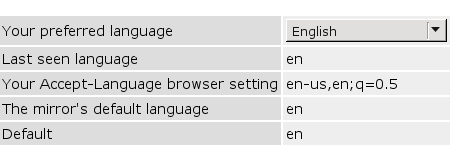
\includegraphics{cap03/language.png}
  \caption{Limba php.net}
  \label{fig:php.net lang}
\end{figure}
Setează-ţi şi următoarele preferinţe:
\begin{itemize}
\item \textbf{URL search fallback} -- Function list search
\item \textbf{Mirror site redirection} -- alege un mirror apropiat de locaţia ta geografică
\end{itemize}
Restul setărilor rămân la atitudinea ta.

Cu Firefox, mai poţi adăuga php.net şi ca motor de căutare, ca în
figura \ref{fig:php.net search}.

\begin{figure}[h!]
  \centering
    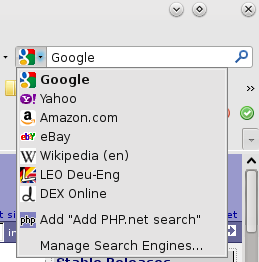
\includegraphics[width=150px]{cap03/search.png}
  \caption{Căutare în manualul PHP cu Firefox}
  \label{fig:php.net search}
\end{figure}

Introdu \textit{var\_dum}p în câmpul de căutare, şi vei fi condus
către pagina din manual a funcţiei. Acolo poţi vedea
în ordine
\begin{itemize}
\item versiunile PHP în care există funcţia
\item o descriere scurtă a funcţiei
\item semnătura funcţiei şi o descriere pe larg
\item eventuale avertizări
\item lista parametrilor şi semnificaţia lor
\item valoarea returnată
\item exemple de utilizare
\item funcţii înrudite
\item comentarii ale altor utilizatori
\end{itemize}
Sunt o grămadă de informaţii. Practic, manualul
PHP conţine toate informaţiile de care ai nevoie.
Din acest motiv cartea de faţă nu încearcă să 
duplice explicaţiile pe care le poţi găsi în manual,
ci doar să te călăuzească. În plus, comentariile
celorlalţi sunt extrem de utile. Foarte rar te vei
afla într-o situaţie unică în care nu s-a mai aflat
nimeni altcineva şi comentariile acelea nu îţi vor fi de 
folos. E recomandat să le citeşti şi pe ele.

\good{Cartea nu va explica toate funcţiile folosite
în listinguri. Când întâlneşti o funcţie nouă,
trebuie să te documentezi din manual.
}
\attention{Ceea ce ţi se va explica în carte sunt conceptele
generale şi termenii, astfel încât să te poţi
descurca singur.}

\subsection{Studiu de caz: funcţii variadice}
După cum observi în manual, funcţia \texttt{var\_dump()}
are de fapt semnătura
\begin{verbatim}
void var_dump (mixed $expression [, mixed $expression [, $... ]])
\end{verbatim}
\ldots înseamnă că funcţia acceptă un număr variabil
de parametri, însă trebuie să fie cel puţin unul.
Astfel de funcţii se numesc funcţii variadice (en. \textsl{variadic}).

\begin{Exercise}[title={Crează o funcţie variadică}]
\ExePart
Caută în manual funcţia \texttt{func\_num\_args()} şi
toate funcţiile înrudite cu ea pentru a crea
o funcţie variadică care returnează produsul parametrilor
pasaţi.

\ExePart
Scrie o nouă versiune a funcţiei care are semnătura
\begin{verbatim}
int array_product(array $numbers)
\end{verbatim}
şi care returnează produsul numerelor salvate în array.

% \ExePart
% 
% Ce observi? Cum poţi îmbunătăţi prima funcţie, cu respect
% faţă de a doua?
% TODO cum? nici eu nu mai ştiu
\end{Exercise}


\subsection{Categoriile de extensii disponibile}
Pe pagina oficială fiind, dacă navighezi către
\texttt{Documentation} $\rightarrow$ \texttt{View online}
$\rightarrow$ \texttt{English},
vei ajunge la indexul
manualului, la pagina sa de start.

Capitolele mari prezentate sunt lucruri precum
\textit{Getting Started} care conţine şi un tutorial,
\textit{Language Reference}, pe care l-ai
citit ca parte dintr-un exerciţiu din capitolul trecut,
\textit{Security} care conţine sfaturi de securitate,
şi asupra cărora vom reveni şi noi
în acest capitol, \textit{Features} îţi prezintă
unele capacităţi ale lui PHP folosite
în mod tipic de aplicaţii, \textit{PHP at the Core: A Hacker's Guide to the Zend Engine}
îţi prezintă inima interpreterului PHP, şi alte câteva capitole.

Deocamdată vrem să ne facem o imagine de ansamblu a funcţiilor
puse la dispoziţie, din capitolul \textit{Function Reference}.

\textit{Affecting PHP's Behaviour} sunt extensii care afectează
modul fundamental de funcţionare al lui PHP. De astfel de funcţii
nu vei avea nevoie decât când ajungi la nivelul avansat. Unele
dintre cele mai des folosite extensii din această categorie sunt
aşa numitele \textit{opcode cachers},
%TODO CHAP which chapter opcode cacher?
asupra cărora vom reveni într-un capitol viitor.

Extensiile pentru \textit{Audio Formats Manipulation} pun
la dispoziţie funcţii pentru formate audio de fişiere şi metadate
salvate în astfel de fişiere.

\textit{Authentication Services} sunt pentru servicii de autentificare,
utile în situaţii destul de complexe în care trebuie să integrezi
autentificarea utilizatorilor în alte servicii deja existente, sau să
faci autentificarea folosind servicii centralizate cu care şi alte aplicaţii pot
comunica.

\textit{Date and Time Related Extensions} conţin funcţii pentru
lucrul cu date şi timp, diferenţa dintre două date, convertirea
de input care reprezintă date sau timp în formate numerice uşor
de înţeles de către calculatoare\footnote{timestamps} sau fuse orare.

\textit{Compression and Archive Extensions} se ocupă de formate
de fişiere precum \texttt{zip} sau \texttt{phar},\footnote{php archive}
un format de arhivare propriu PHP care-ţi permite să incluzi aplicaţii
întregi dintr-un singur foc, chiar dacă acestea conţin câteva mii
de fişiere cu cod sursă.

\textit{Credit Card Processing} sunt pentru procesarea cărţilor de credit.

\textit{Cryptography Extensions} sunt utile atunci când vrei să
criptezi informaţii importante, precum numerele de conturi pe care le
procesezi cu funcţiile de procesare ale cărţilor de credit.

\textit{Database Extensions} pun la dispoziţie extensii pentru
comunicarea cu baze de date. MySQL este unul dintre cele mai folosite
sisteme de management al bazelor de date în aplicaţiile
PHP, însă există o grămadă de alte sisteme pentru organizarea
structurată a informaţiilor.

\textit{File System Related Extensions} se ocupă cu lucrul cu
fişiere şi directoare, citirea sau scrierea din/în fişiere,
listarea fişierelor dintr-un director, informaţii despre fişiere
precum drepturile de acces sau posesorii acestora.

\textit{Human Language and Character Encoding Support} sunt
printre altele pentru internaţionalizarea aplicaţiilor.
Dacă vrei să faci o aplicaţie cu interfaţa în mai multe
limbi, atunci trebuie să apelezi la funcţionalităţile
puse la dispoziţie de aceste extensii.

\textit{Image Processing and Generation} sunt pentru
prelucrarea şi generarea programatică a imaginilor.

\textit{Mail Related Extensions} sunt pentru
lucrul cu diferite protocoluri sau formate de e-mail.

\textit{Mathematical Extensions} pun la dispoziţie
funcţii matematice.

HTML este un limbaj bazat pe text.
\textit{Non-Text MIME Output} se ocupă cu
generarea de documente sau resurse în alte formate pe
lângă text precum animaţii flash sau documente PDF.

Funcţiile din extensiile de \textit{Process Control Extensions}
îţi permit să lansezi în execuţie alte programe cu interfaţă
CLI şi să
comunici cu acestea fie citind şi scriind din/în outputul/inputul
acelor procese, fie prin alte mecanisme precum IPC
(en. \textsl{inter-process communication}).

\textit{Other Basic Extensions} sunt extensii care pun
la dispoziţie diferite funcţionalităţi de bază.
Cele mai des întâlnite şi folosite sunt cele din
extensia \textit{URLs} şi din extensia \textit{Miscellaneous Functions}.

\textit{Other Services} conţine o mulţime de extensii. Una dintre
cele mai comune este \textit{sockets}. Cu ea poţi deschide
conexiuni programatic, aşa cum ai făcut cu telnet, şi transfera
date (în orice protocol, nu numai HTTP). Altă extensie folosită des
este \textit{cURL}, cu care poţi deschide conexiuni HTTP, fără
a fi nevoit să creezi manual cererile HTTP, aşa cum ai face-o cu
\textit{sockets}.

\textit{Search Engine Extensions} sunt extensii care te lasă
să comunici cu alţi daemoni care au menirea de a indexa
fişiere şi de a te lăsa să cauţi după cuvinte cheie de
exemplu. Majoritatea aplicaţiilor comune scrise în PHP
nu folosesc aceste servicii deoarece pentru aplicaţii mici
necesită prea multe resurse. Ele salvează datele în baze de
date, de obicei MySQL, şi caută manual. Aceste extensii
pentru \textit{search engine} sunt totuşi foarte
utile când vrei să faci ceva extensibil, fără a pune
presiune pe o bază de date. Ele reprezintă de fapt moduri "corecte"
de a implementa funcţionalitatea de căutare pe un site.

\textit{Server Specific Extensions} pun la dispoziţie
funcţii specifice SAPI-ului folosit. Dacă ai instalat
şi configurat mediul de programare ca în capitolul 1,
atunci foloseşti SAPI-ul Apache.

\textit{Session Extensions} pun la dispoziţie funcţionalitatea
numită \textsl{sesiuni}. Sesiunile permit aplicaţiilor web
să "ţină minte" utilizatorii şi date asociate cu aceştia.
Mulţumită sesiunilor este posibilă autentificarea utilizatorilor.

Categoria \textit{Text Processing} conţine extensii pentru
lucrul cu text, cu stringuri. Cele mai folosite extensii
din această categorie sunt \textit{Strings} pentru operaţii
cu stringuri precum căutare, stabilirea lungimii, ş.a.m.d.
şi \textit{PCRE} (en. \textsl{perl-compatible regular expressions}).
PCRE îţi permite să verifici dacă un string potriveşte o
regulă\footnote{Aşa cum ai inventat o regulă pentru
sintaxa limbajului HTML în capitolul 2} şi eventual
să şi extragi anumite secvenţe din acel string.\\
PCRE este puternic, dar consumă şi multe resurse,
deci este recomandat să foloseşti funcţiile simple
din extensia \textit{Strings} atunci când e posibil.

\textit{Variable and Type Related Extensions} pun
la dispoziţie funcţii pentru lucrul cu tipurile
de date fundamentale din PHP (în afară de stringuri,
care sunt tratate de extensiile prezentate anterior), printre
care array-uri, funcţii şi variabile. Atunci când ai căutat
informaţii despre funcţia \texttt{func\_num\_args()}
şi funcţiile înrudite cu ea, te-ai mişcat prin extensia
\textit{Function Handling}.

Extensiile din categoria \textit{Web Services} sunt folosite
pentru a crea şi folosi servicii web. Atunci când aplicaţia
ta pune la dispoziţie un serviciu web, aceasta poate
fi contactată de alte aplicaţii şi informaţiile pot
fi procesate programatic mult mai uşor. Acelaşi lucru îl
poţi face şi tu cu alte aplicaţii care îşi oferă
funcţionalităţile şi ca servicii web. De exemplu,
reţelele sociale precum Facebook\footnote{\url{http://facebook.com/}}
sau Twitter\footnote{\url{http://twitter.com/}} pun la dispoziţie
astfel de servicii. Asta le permite altor programatori să
creeze programe care postează tweet-uri pe twitter sau
jocuri pe care le poţi juca împreună cu prietenii tăi
pe facebook, aplicaţii care nu au legătură directă
cu firmele originale precum twitter sau facebook în
cazul nostru.

\textit{Windows Only Extensions} pun la dispoziţie funcţionalităţi
specifice Microsoft Windows. Acestea nu vor funcţiona decât dacă
daemonul cu PHP integrat în el rulează pe windows.
Este recomandat să nu foloseşti astfel de funcţii
decât în cazul în care ştii sigur că aplicaţia ta
va rula într-un mediu controlat, pe windows, deoarece
majoritatea serverelor rulează pe o formă sau alta
de *NIX\footnote{GNU/Linux, *BSD, SunOS, etc}, nu Windows.

\textit{XML Manipulation} pune la dispoziţie funcţionalitate
pentru lucrul cu fişiere în formatul XML. XML este un format
care-ţi permite să structurezi informaţii arborescente. Din punct
de vedere sintactic este
similar cu HTML, iar combinaţia dintre HTML şi XML a dat naştere
limbajului XHTML. În contrast cu (X)HTML însă, XML nu are
"taguri" predefinite. Programatorii îşi inventează
propriile formate de date şi le dau o semnificaţie.

Acestea au fost categoriile de extensii disponibile în PHP.
Unele dintre ele vin la pachet cu PHP, altele se află
în ceea ce numim PECL (en. \textsl{PHP Extension Community Library})
şi trebuie instalate separat.

Nu uita că deşi fac parte din aceeaşi categorie, două extensii nu
pot comunica una cu alta. De exemplu, dacă ai stabilit o conexiune
cu o bază de date MySQL, atunci nu poţi pasa această conexiune
unei funcţii care lucrează cu baze de date PostgreSQL. Cele două
extensii sunt complet diferite şi independente. Categorisirea
extensiilor este doar modul de organizare a informaţiilor în
manualul PHP, pentru o navigare mai uşoară.


\subsection{Extensii de bază}
În categoria \textit{Variable and Type Related Extensions}
este o extensie cu funcţii pentru lucrul cu array-uri.
Dacă urmezi link-ul \textit{Array Functions} vei vedea
indexul tuturor funcţiilor pentru array-uri alături de
o descriere scurtă a fiecăreia.

\begin{Exercise}[title={Înţelege manualul}]
Alege cinci funcţii de lucru cu array-uri şi
explică în cuvinte ce face fiecare, apoi crează
unul sau mai multe coduri sursă care să le demonstreze
utilitatea.
\end{Exercise}
\begin{Exercise}[difficulty=3,title={Explorează manualul}]
În acest moment ai o privire destul de robustă a
limbajului, dar nu ştii funcţiile care-ţi sunt
puse la dispoziţie. Totuşi, mulţumită explicaţiilor
de până acum, eşti capabil să înţelegi manualul.

Rezervă-ţi 40-80 de ore (1-2 săptămâni de lucru)
pentru a explora următoarele extensii:
\begin{itemize}
\item \textit{Array},
\textit{Function Handling}, \textit{Variable Handling} din categoria \textit{Variable and Type Related Extensions}
\item \textit{Strings} din categoria \textit{Text Processing}
\item \textit{Miscellaneous Functions} din categoria \textit{Other Basic Extensions}
\end{itemize}
Scrie scripturi de la simple la complexe care se folosesc
de aceste funcţii. Documentează-ţi scripturile cu comentarii.
La fiecare script scrie şi ce-ţi trece prin minte, ce observaţii
ai făcut, ce legături sau analogii ai făcut.

Nu uita să separi \textit{business logic} de \textit{view logic} şi să transmiţi date ce
rezultă în urma procesării formularelor (\textit{business logic}) către \textit{view logic}
folosind \textit{variabile intermediare}.

Postează fiecare cod sursă pe {\phpro} pentru a te verifica pe parcursul
celor 1-2 săptămâni, încă din momentul în care ai scris ceva nou.\footnote{Nu toate
scripturile deodată} În total ar trebui să ai câteva zeci bune de scripturi, cu
până la 1000 de LOCs sau chiar mai mult.

La fiecare exerciţiu explică modul de funcţionare \^in ceva asemănător cu
limbaj pseudocod, dar fără a folosi identificatori de variabile
sau a reflecta exact structura codului. Explică \^in schimb motivaţiile
de a proceda \^intr-un anumit fel.

Crează un jurnal al tuturor funcţiilor despre care te-ai documentat
singur din manual, cu semnătura funcţiei şi o explicaţie scurtă
despre ce face\footnote{Explicaţii scurte se pot găsi pe indexul
funcţiilor din manualul PHP.}.

După aceste 1-2 săptămâni nu îţi va mai sta nimic în calea creării
de site-uri destul de complexe {\ldots} cu câteva mici excepţii pe care le vom
aborda \^in cele ce urmează.
\end{Exercise}



%TODO ce altfel de explicaţii aş mai putea adăuga pentru a clarifica ev. nelămuriri?
%TODO pune-i pe cursanţi să înveţe din manual lucruri ca lucrul cu fs sau printf() & co şi observă dificultăţile





\section{Structuri de date}
Array-urile sunt atât de versatile încât pot fi folosite
pentru a construi structuri de date mai complicate, fiecare
cu avantajele şi dezavantajele sale.

\subsection{Stack şi queue}
Un \textsl{stack} este un array în care elementele sunt adăugate la sfârşit,
şi preluate tot de la sfârşit. Operaţia de adăugare a unui element
pe \textit{stack} se numeşte \textsl{push}, iar cea de scoatere se numeşte \textsl{pop}.

Un \textit{stack} poate fi reprezentat vizual ca în figura \ref{fig:stack}.

\begin{figure}[h!]
  \centering
    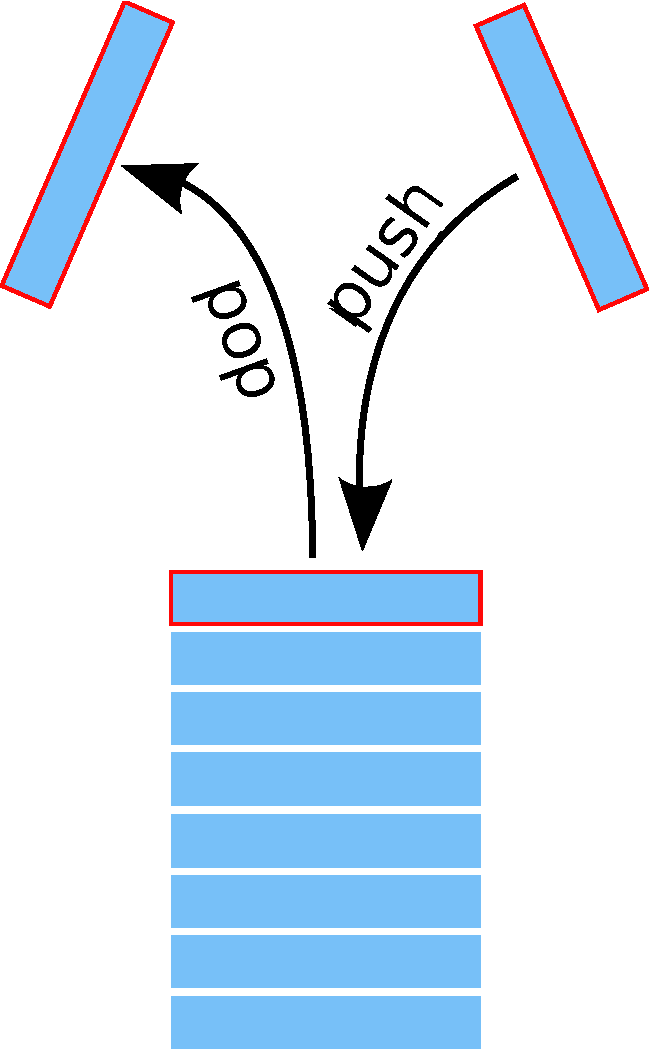
\includegraphics[scale=.3]{cap03/stack-crop.pdf}
  \caption{Operaţiile cu un stack}
  \label{fig:stack}
\end{figure}

Deoarece ultimul element adăugat este primul care este îndepărtat
din \textit{stack}, spunem că un \textit{stack} este o structură de date
de tip \textsl{LIFO} (en. \textsl{last in, first out}).

Operaţia \textit{push} îţi este cunoscută deja prin intermediul
operatorului \texttt{[]} pe care l-ai întâlnit în
listingul \ref{lst:push_operator}. Există şi o funcţie
absolut echivalentă în funcţionalitate cu acesta: \texttt{array\_push()}.

Similar cu LIFO, există şi FIFO (en. \textsl{first in, first out}),
numit şi \textsl{queue}. Operaţiile se numesc \textsl{shift} şi \textsl{unshift},
iar grafic ne putem imagina o astfel de structură de date ca în
figura \ref{fig:queue}.

\begin{figure}[h!]
  \centering
    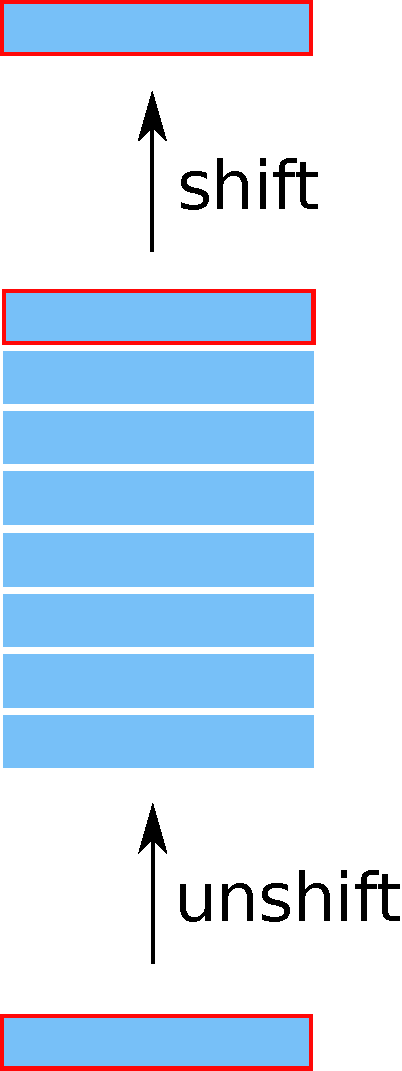
\includegraphics[scale=.3]{cap03/queue-crop.pdf}
  \caption{Operaţiile cu un queue}
  \label{fig:queue}
\end{figure}

Primul element pus în \textit{queue} este primul
element care va fi îndepărtat din \textsl{queue}.

Pentru aceste două operaţii există două funcţii numite
destul de intuitiv \texttt{array\_shift()} şi
\texttt{array\_unshift()}.



\begin{Exercise}[title={Experimentează cu stack şi queue}]
Scrie un script complet în care experimentezi cu
aceste structuri de date. Nu uita că poţi trata
acelaşi array alternativ, când ca \textit{stack}, când ca \textit{queue}.
\end{Exercise}

\subsection{Structuri de date recursive}
În exerciţiul \ref{ex:sintaxa_html} \textit{Sintaxa HTML} ai
făcut cunoştinţă cu recursivitatea. În PHP poţi procesa
structuri de date recursive folosind funcţii recursive.
De exemplu,
un document HTML este o structură de date recursivă
deoarece nodurile din
document\footnote{DOM - \href{http://en.wikipedia.org/wiki/Document_Object_Model}{document object model}}
pot avea în interiorul lor alte noduri. Din acest motiv
spunem că structurile de date recursive sunt şi izomorfice.

În capitolul trecut ai văzut cum poţi construi array-uri
n-dimensionale, unde n era bine determinat.

Un array recursiv este constituit, la fel ca şi un array
n-dimensional, din alte array-uri. Diferenţa este că
n nu este determinat. Trebuie să parcurgem recursiv
array-ul pentru a procesa fiecare element.

%TODO file cap03/family-tree* no longer needed

Vom lua ca exemplu un array recursiv:
\begin{lstlisting}
<?php
$arbore = array(
  'hello',
  'foo',
  'world' => array(
        'how',
        'are',
        'you',
        'today?' => array(
          'march',
          27,
          2010
        )
  ),
  'out',
  'there!'
);

foreach($arbore as $k => $v) {
  if(is_string($v)) {
	echo "$k => $v";
  }
  elseif(is_array($v)) {
	echo " *** RECURSIVITY";
  }
  echo PHP_EOL;
}
\end{lstlisting}
Practic nu este nimic nou. Iterăm array-ul şi afişăm
valorile. Însă pe linia 23 detectăm dacă valoarea însăşi
este la rândul ei tot un array (precum \texttt{\$arbore},
pe care tocmai îl iterăm), şi afişăm \texttt{" *** RECURSIVITY"}.

Ţin să subliniez: valoarea \$v este un array, şi chiar
dacă se află în interiorul unui array \$arbore, este tot un
array, deci \$v poate fi iterat cu exact aceeaşi buclă
\texttt{foreach}
cu care iterăm \$arbore.

Practic, nu trebuie decât să reutilizăm codul de pe liniile
19-27. Şi ce modalitate cunoaştem pentru a reutiliza codul?
Exact, funcţiile!

Deci implementăm o funcţie
\begin{verbatim}
void itereaza_recursiv(array $arbore)
\end{verbatim}
şi o apelăm, astfel:
\begin{lstlisting}
<?php
$arbore = array(
  'hello',
  'foo',
  'world' => array(
        'how',
        'are',
        'you',
        'today?' => array(
          'march',
          27,
          2010
        )
  ),
  'out',
  'there!'
);

function itereaza_recursiv($arbore) {
  foreach($arbore as $k => $v) {
        if(is_string($v) || is_numeric($v)) {
          echo "$k => $v";
          echo PHP_EOL;
        }
        elseif(is_array($v)) {
          echo "going into '$k'\r\n";
          itereaza_recursiv($v);
        }
  }
}

itereaza_recursiv($arbore);
\end{lstlisting}
După cum observi, funcţia \texttt{itereaza\_recursiv()} se apelează
pe ea însăşi pe linia 27, însă cu o altă valoare -- cu
valoarea elementului curent \$v, care este tot un array.
Pe linia 27 spunem că intrăm în recursivitate. La primul apel,
la elementul \texttt{'world'}, intrăm în adâncimea 1
a arborelui. În cadrul elementului \texttt{'world'}
se află încă un element la cheia \texttt{'today?'}
care are ca valoare un array. Atunci când se ajunge la el,
spunem că intrăm în adâncimea 2 "a recursivităţii".

După ce am afişat valoarea \texttt{2010}, ieşim din recursivitatea
de adâncime 2, revenind la 1, şi ne aflăm iar în array-ul cu
cheia \texttt{'world'}. Însă ajunşi aici, ne aflăm iar
la sfârşitul iteraţiei, deoarece bucla \texttt{foreach}
ajunge la sfârşitul array-ului salvat în elementul \texttt{'world'},
deci ieşim din recursivitate (şi deci din funcţia \texttt{itereaza\_recursiv()}),
revenind \ldots tot în funcţia \texttt{itereaza\_recursiv()}!

Însă acum ne aflăm pe linia 28, şi nu ne aflăm la sfârşitul recursivităţii
de "adâncime" 0, deci bucla foreach trece la următorul element: \texttt{'out'}.



\begin{Exercise}[title={Adâncimea recursivităţii},difficulty=2]
Modifică funcţia \texttt{itereaza\_recursiv()} dându-i semnătura:
\begin{verbatim}
string itereaza_recursiv(array $arbore, $depth=0)
\end{verbatim}
şi modifică implementaţia astfel încât fiecare afişare
de forma \texttt{"cheie => valoare"} să aibă în faţa sa
un număr de spaţii egal cu adâncimea din recursivitate la care
se află acel element, structura arborescentă fiind
astfel evidenţiată şi grafic:
\begin{verbatim}
0 => hello
1 => foo
going into 'world'
  0 => how
  1 => are
  2 => you
  going into 'today?'
    0 => march
    1 => 27
    2 => 2010
2 => out
3 => there!
\end{verbatim}
Funcţia nu trebuie să afişeze direct cu \texttt{echo},
ci să returneze outputul ca string, din motive
de modularizare.

Scriptul trebuie să funcţioneze ca script CLI,
nu printr-un daemon http, deci pentru a genera
o linie nouă în output foloseşte constanta
\texttt{PHP\_EOL}, pe care o cunoşti deja.
\end{Exercise}

Până acum am lucrat cu propriile structuri de date
recursive. Vei fi confruntat deseori cu necesitatea
de a inventa astfel de structuri de date, însă
şi mai des va trebui să procesezi date recursive
asupra cărora nu ai control. Un astfel
de exemplu este un director, căci un director poate avea
fişiere şi alte directoare în el. Observi recursivitatea?

Lucrul cu fişiere şi directoare se poate face
cu ajutorul extensiilor din categoria
\textit{File System Related Extensions}, mai exact
ne interesează în special extensia \textit{Directory Functions}.
Din extensia \textit{Filesystem Functions} avem nevoie
doar de funcţiile \texttt{is\_dir()} şi \texttt{is\_file()}
pentru a verifica dacă un element este director sau
fişier.

Începem prin doar a itera un director, fără
a intra recursiv în alte subdirectoare:

\begin{lstlisting}
<?php
function display_directory($dirpath) {
  $dh = opendir($dirpath);
  while($entry = readdir($dh)) {
	echo $entry;
	if(is_dir($dirpath.DIRECTORY_SEPARATOR.$entry)) {
	  echo DIRECTORY_SEPARATOR;
	}
	echo PHP_EOL;
  }
  closedir($dh);
}

display_directory(__DIR__);
\end{lstlisting}
\texttt{opendir()} ne returnează o resursă. Acesta este
un alt tip de date fundamental în PHP, însă
el nu poate fi creat direct de scripturile noastre,
ci doar prin intermediul funcţiilor native PHP,
implementate în extensii.

Deschizând un director cu \texttt{opendir()} avem
acces la această resursă şi îl putem itera.

Cu \texttt{readdir()} citim fiecare intrare din acest
director, salvând rezultatul în \texttt{\$entry}.
Această variabilă este fie un string, fie FALSE,
dacă am iterat totul, caz în care condiţia buclei
\texttt{while} va fi FALSE, deci se va ieşi din
bucla din fluxul de execuţie.

Pe linia 6 verificăm dacă noua intrare este un
director, şi dacă da, afişăm şi valoarea
constantă \texttt{DIRECTORY\_SEPARATOR}.
Diferite sisteme de operare folosesc diferite
separatoare în căile către fişiere şi directoare.
MS Windows foloseşte \texttt{\textbackslash}, în timp ce GNU/Linux
foloseşte \texttt{/}. Constanta \texttt{DIRECTORY\_SEPARATOR}
va avea mereu valoarea corespunzătoare platformei
pe care rulează scriptul.

Afişarea acestei
constante este doar un indiciu vizual pentru noi,
să ştim dacă avem de-a face cu un fişier, sau cu un
director. În practică, aici ar trebui să
intrăm recursiv în noul subdirector.

Toate\footnote{Aproape toate} directoarele
au două pseudo-directoare în ele: \texttt{'.'}
şi \texttt{'..'}. Acestea nu sunt directoare
în adevăratul sens al cuvântului, ci sunt referinţe,
primul către directorul însuşi, al doilea către
directorul părinte. Cu siguranţă ai folosit
deja în HTML căi relative precum
\begin{lstlisting}[language=HTML]
<img src="../img/me.jpg">
\end{lstlisting}
De aici vine acel \texttt{'..'}.

\begin{Exercise}[title={Determinarea recursivă a conţinutului unui director},difficulty=2]
În funcţia anterioară, în loc de simpla afişare
a valorii \texttt{DIRECTORY\_SEPARATOR}, vrem să intrăm în
directorul respectiv. Extinde şi modifică funcţia
astfel încât să aibă semnătura
\begin{verbatim}
array get_directory_structure(string $dir_path)
\end{verbatim}
şi să returneze fişierele şi toate subdirectoarele din
directorul \$dir\_path într-un array recursiv.
\end{Exercise}

\begin{Exercise}[title={Afişarea unei structuri de date recursive},difficulty=1]
\ExePart

Implementează o funcţie
\begin{verbatim}
string render_recursive_array_to_ul(array $array)
\end{verbatim}
care acceptă ca parametru un array (eventual recursiv) şi returnează
reprezentarea HTML a acestuia într-o listă neordonată (\texttt{<ul>}).

Acestei funcţii îi vei putea pasa valoarea returnată
de un apel la \texttt{get\_directory\_structure()} implementată
în exerciţiul anterior.

Observi cum implementaţia de funcţii care operează
doar pe date abstracte (aici: array-uri) duc
automat la reutilizarea şi o mai bună
modularizare a codului?

\ExePart

Extinde funcţia astfel încât să accepte şi o funcţie anonimă
ca \textit{callback}:
\begin{verbatim}
string render_recursive_array_to_ul(array $array,callback $cb=NULL)
\end{verbatim}
care dacă este prezent, este folosit pentru a genera outputul
ce trebuie pus între \texttt{<li>} şi \texttt{</li>}.
Semnătura callback-ului trebuie să fie
\begin{verbatim}
string cb(string $path)
\end{verbatim}
\end{Exercise}

\section{Call Stack}
Atunci când apelăm o funcţie, PHP pune contextul actual de execuţie
pe un stack (operaţia \textit{push}), şi apoi se apelează funcţia.
La ieşirea din funcţie (cu un \texttt{return}), PHP face un
\textit{pop} pentru acel stack, şi execuţia se continuă de unde
fusese întreruptă anterior.

Acest stack se numeşte \textsl{call stack}, fiecare element
de pe acest stack fiind numit \textsl{call frame}.
\section{Fişiere multiple}
Până acum ne-am structurat scripturile în funcţii reutilizabile pe de o parte,
şi pe de alta separând \textit{business logic} de \textit{view logic}, însă
totul se afla într-un singur fişier. Nu puteam refolosi nici logica, nici
prezentarea, separate una de alta.

PHP ne pune la dispoziţie patru directive pentru includerea unui fişier în
alt fişier .php. Primele două se numesc \texttt{include} şi \texttt{require}.
Sintaxa este destul de intuitivă:
\begin{verbatim}
include <string>;
require <string>;
\end{verbatim}

Exemplu:
\begin{lstlisting}[title=index.php]
<?php
if(isset($_GET['nume']) && is_string($_GET['nume'])) {
  $nume = $_GET['nume'];
}

if(isset($nume)) {
  include 'greet_nume.php';
}
include 'greeting_form.php';
\end{lstlisting}
\begin{lstlisting}[title=greet\_nume.php]
Salut <?php echo $nume; ?>.
\end{lstlisting}
\begin{lstlisting}[title=greeting\_form.php,language=html]
<form method="GET" action="index.php">
  <input type="text" name="nume" />
  <input type="submit" value="greet" />
</form>
\end{lstlisting}

Bineînţeles exemplul nostru nu este atât de complex încât 
avantajele să devină evidente. Un avantaj posibil ar fi că putem schimba modul
de funcţionare extrem de uşor, fără a modifica nici un alt
fişier în afara lui \texttt{index.php}.

Aşa cum este acum, scriptul afişează formularul indiferent
dacă avem numele ca input sau nu. Am putea schimba rapid în afişarea
formularului doar dacă numele nu a fost trimis de utilizator, modificând
\texttt{index.php} astfel:
\begin{lstlisting}[title=index.php,firstnumber=6]
if(isset($nume)) {
  include 'greet_nume.php';
}
else {
  include 'greeting_form.php';
}
\end{lstlisting}
fără a ne atinge de nici un alt fişier.

Alt avantaj e că am putea refolosi \texttt{greet\_nume.php} oricând
vrem să salutăm pe cineva. Nu ar trebui decât să ne asigurăm că există variabila
\texttt{\$nume}, deoarece aceasta este folosită de acel script.

Diferenţa dintre \texttt{include} şi \texttt{require} constă în cum
tratează PHP absenţa fişierului inclus. Cu \texttt{include}, PHP generează
o avertizare dar continuă execuţia. Cu \texttt{require}, execuţia se opreşte
complet dacă fişierul nu există sau PHP nu îl poate citi. De aceea,
este recomandat să folosim \texttt{require} atunci când ştim că aplicaţia
nu ar avea oricum să-şi îndeplinească (măcar parţial) execuţia fără
fişierul php pe care vrem să-l injectăm în runtime-ul php.

\attention{Sub MS Windows, \textbackslash trebuie precedat de un alt \textbackslash
în stringurile interpolate atunci când sunt declarate căi pentru filesystem.}

Celelalte două directive pentru includerea codului de fişiere este familia
\texttt{*\_once}. Sintaxa:
\begin{verbatim}
include_once <string>;
require_once <string>;
\end{verbatim}
Aşa cum le spune şi numele, aceste constructe vor include fişierul doar o singură
dată. Asta este foarte util dacă fişierul inclus conţine implementările unor funcţii,
deoarece, dacă am implementa o funcţie cu acelaşi nume de mai multe ori, PHP
ne-ar spune că nu putem redeclara acea funcţie. Exemplu:
\begin{lstlisting}
<?php
include_once 'functions.php';
include_once 'functions.php';//nu va mai fi inclus inca o data
echo foo();
\end{lstlisting}
Unde funcţia \texttt{foo()} este implementată în fişierul \texttt{functions.php}.
Totuşi în acest caz ar fi mai bine să folosim \texttt{require\_once}, astfel încât dacă
fişierul \texttt{functions.php} nu există, execuţia să fie întreruptă din start.
Nu are rost să încercăm să executăm un cod care apelează o funcţie care nu există,
deoarece fişierul în care ar trebui să fie implementată nu există.

\subsection{Şabloane}
În exemplul anterior, \texttt{greet\_nume.php} se numeşte \engl{şablon}{template}.
Folosirea lui este însă dependentă de existenţa unei variabile numită \texttt{\$nume},
ceea ce face \textit{template}-ul nostru să fie cuplat de această variabilă, la fel
cum şi cuvântul cheie \texttt{global} cuplează numele unei variabile de o funcţie.

Putem decupla foarte elegant orice template de variabilele folosite
în el creând o funcţie precum:
\begin{verbatim}
void render(string $template, array $vars=NULL)
\end{verbatim}
unde \texttt{\$template} este calea către un fişier .php folosit
ca template, iar \texttt{\$vars} este un array asociativ. Acest array
va fi iterat ca în listingul \ref{lst:varvarfromassoc}, creând astfel
variabilele cerute de template-ul \texttt{\$template}. Aceste variabile
vor fi locale funcţiei \texttt{render()},\footnote{Se vor afla doar în scope-ul local
al funcţiei} deci nu vor polua nici un scope, fiind şterse automat de PHP
atunci când fluxul de execuţie iese din funcţie. În acelaşi timp, variabilele
specifice template-ului nu vor fi cuplate de \textit{scope}-ul global, aşa cum \texttt{\$nume}
folosit de \texttt{greet\_nume.php} era cuplat de \texttt{\$nume} din \textit{scope}-ul
global (\texttt{index.php}).

După ce variabilele variabile
au fost create, o simplă instrucţiune de includere a fişierului va genera outputul.

Dacă funcţia nu primeşte un al doilea parametru de la apelant, atunci \texttt{\$vars}
va avea valoarea \texttt{NULL}, şi nu ar trebui să mai creăm variabilele variabile,
ci doar să includem \textit{template}-ul.

\begin{Exercise}[title={O funcţie render()}]
\ExePart
Scrie o funcţie
\begin{verbatim}
void render(string $template, array $vars=NULL)
\end{verbatim}
care crează variabile variabile pe baza array-ului asociativ \$vars
şi apoi include \$template.

Exemplu de apelare a acestei funcţii:
\begin{lstlisting}
render('greet_nume.php',array('nume' => $nume));
\end{lstlisting}

\ExePart

Rescrie funcţia \texttt{render()} folosind funcţia internă
\texttt{extract()}.
%TODO WIKI: explică ce e o funcţie internă şi că trebuie înlocuit cu foreach
\end{Exercise}
În exemplul din exerciţiul anterior am apelat funcţia cu parametrul
\texttt{array('nume' => \$nume)}. În PHP există funcţia \texttt{compact()}
care poate crea un array asociativ cu numele variabilelor ca chei, şi
valorile acestora ca valori în array. Este o funcţie foarte utilă
atunci când numele variabilelor din \textit{scope}-ul actual (în cazul de
faţă cel global) sunt numite la fel ca variabilele folosite în
\textit{template}-ul în cauză.


\subsection{Primul site complet}
Hai să vedem cum putem folosi toate lucrurile învăţate sau nu până acum. Includ
şi lucrurile neînvăţate, deoarece mă aştept să te documentezi din manual
atunci când întâlneşti o funcţie necunoscută.

O vom lua gradual, adăugând treptat funcţionalitate, şi deci şi complexitate.

Vrem să facem un site personal cu câteva pagini. Întregul site va prezenta
pe toate paginile un meniu comun cu lista paginilor existente. 

\begin{figure}[H]
  \centering
    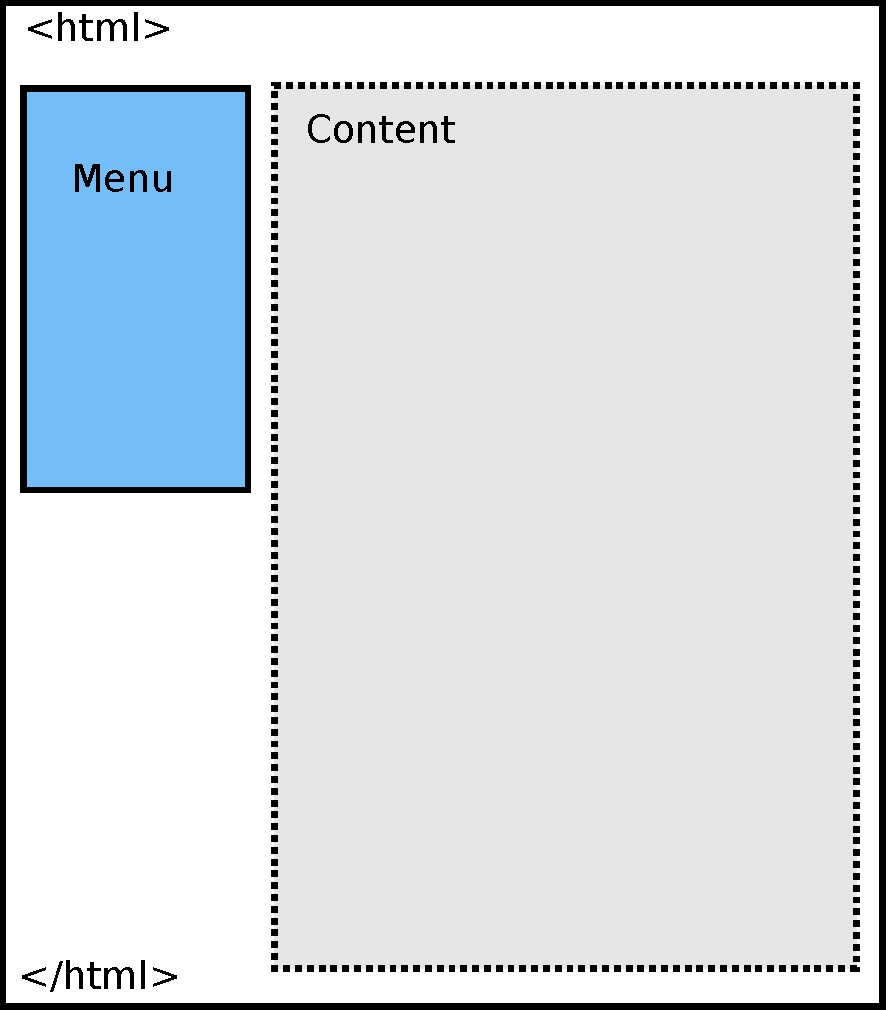
\includegraphics[scale=.5]{cap03/homepage-layout-crop.pdf}
  \caption{Layout site personal}
  \label{fig:layout site personal}
\end{figure}

Toate paginile vor
arăta similar, doar conţinutul efectiv al fiecărei pagini fiind diferit. Spunem că site-ul
foloseşte un \textit{template}. Acesta va arăta ca în figura \ref{fig:layout site personal}.


\begin{Exercise}[title={Crează template}]
Crează un fişier XHTML 1.1 structurat ca
în figura \ref{fig:layout site personal}. Alegerea culorilor şi aşezarea
în pagină sunt lăsate la atitudinea ta, dar meniul trebuie să fie
definit aşa:
\begin{lstlisting}[language=html]
<div id="menu">

</div>
\end{lstlisting}
iar continutul aşa:
\begin{lstlisting}[language=html]
<div id="content">

</div>
\end{lstlisting}
\end{Exercise}

Pentru site-ul nostru,
am fi tentaţi să punem acest \textit{template} în \texttt{index.php}.
Asta nu ar fi o decizie bună, deoarece nu am putea reutiliza \textit{template}-ul
în alte locuri. \texttt{index.php} ar trebui doar să coordoneze
conlucrarea dintre \textit{business logic} şi \textit{view logic}.
Deci pune template-ul creat într-un fişier nou numit \texttt{layout.php}.
Acum creăm şi index.php, care va afişa template-ul. Ulterior urmează să adăugăm
şi procesările (\textit{business logic}) corespunzătoare:
\begin{lstlisting}[title=index.php]
<?php
require_once 'functions.php';
//here be processing

render('layout.php');
\end{lstlisting}
Crează şi fişierul \texttt{functions.php} şi pune
în el implementaţia funcţiei \texttt{render()} creată
în unul din exerciţiile anterioare.

Acum hai să facem layout-ul să folosească câteva variabile:
\texttt{\$title}, \texttt{\$menu}, şi \texttt{\$content}.
Înlocuieşte astfel încât să ajungi la:
\begin{lstlisting}[numbers=none]
<title><?php echo $title;?></title>
\end{lstlisting}
\begin{lstlisting}[numbers=none]
<div id="menu"><?php echo $menu;?></div>
\end{lstlisting}
şi
\begin{lstlisting}[numbers=none]
<div id="content"><?php echo $content;?></div>
\end{lstlisting}

Deoarece \textit{template}-ul foloseşte acum aceste
variabile, trebuie să i le exportăm. Deci adaugă
un array asociativ corespunzător:
\begin{lstlisting}[title=index.php]
<?php
require_once 'functions.php';
$tpl_vars = array(
  'title' => 'My Homepage',
  'menu' => 'no menu yet',
  'content' => 'no content yet'
);

render('layout.php',$tpl_vars);
\end{lstlisting}

Însă am spus că vrem să afişăm diferite pagini, fiecare pagină cu conţinutul ei, şi
în plus fiecare pagină să aibă un link în meniu.

Cu siguranţă ne-am putea apuca să mâzgălim nişte cod la grămadă, şi cu siguranţă
ne va ieşi ceva aspectuos. Dar cel mai probabil nu ne va ieşi ceva reutilizabil
dacă nu stăm să ne gândim puţin mai profund şi mai sistematic de ce avem nevoie.

Încă o dată, rezumăm: o pagină are
\begin{itemize}
\item un titlu, pus în <title></title> în template
\item un conţinut
\item un meniu
\end{itemize}
În exemplul de mai sus, conţinutul este la noi un string. Însă acest conţinut
va diferi de la pagină la pagină, şi cel mai probabil va fi foarte lung.

Am putea teoretic să punem conţinutul fiecărei pagini într-un string, însă
asta ar face codul foarte greu de citit şi mentenat. Mult mai curat ar fi
dacă am considera un nume de fişier ca fiind caracteristica "conţinut"
a acelei pagini. Altfel spus, o pagină ar consista din:
\begin{itemize}
\item un titlu, pus în <title></title> în template
\item un fişier cu conţinutul efectiv
\item un meniu
\end{itemize}
Deci am putea crea o structură de date abstractă care să conţină o pagină.
Deoarece avem o serie de trei caracteristici pentru o pagină, putem
salva aceste informaţii despre fiecare pagină într-un array asociativ:
\begin{lstlisting}
$home = array(
  'title' => 'Bine ai venit',
  'content' => 'home.php',
  'menu' => 'no menu yet'
);
$about = array(
  'title' => 'Despre mine',
  'content' => 'despre.php',
  'menu' => 'no menu yet'
);
\end{lstlisting}
Nu m-am grăbit să creez şi meniul pentru fiecare pagină, deoarece
am realizat că acest meniu ar putea fi determinat programatic, pe baza
variabilelor precum \texttt{\$home} sau \texttt{\$about}. Ce ar implica
generarea automată a meniului pentru fiecare pagină? Exact! Ar
implica iterarea acestor variabile. Însă noi nu putem itera variabile.
Putem itera array-uri. De aici ne vine ideea genială de a salva toate
paginile într-un array asociativ. 
Hai să vedem cum va arăta \texttt{index.php}

\begin{lstlisting}
<?php
require_once 'functions.php';

$pages = array(
  'home' => array(
	'title' => 'Bine ai venit',
	'content' => 'home.php',
	'menu' => 'no menu yet'
  ),
  'about' => array(
	'title' => 'Despre mine',
	'content' => 'despre.php',
	'menu' => 'no menu yet'
  )
);

$tpl_vars = array(
  'title' => 'My Homepage',
  'menu' => 'no menu yet',
  'content' => 'no content yet'
);

render('layout.php',$tpl_vars);
\end{lstlisting}
Realizăm două lucruri:
\begin{itemize}
\item variabila \texttt{\$tpl\_vars} devine inutilă -- toate informaţiile se află acum în \texttt{\$pages},
chiar dacă nu în exact aceeaşi formă. De exemplu, va trebui să găsim o metodă de a "citi" fişierul .php
cu conţinutul, deoarece nu vom mai avea la dispoziţie conţinutul efectiv ca string
\item variabila \texttt{\$pages} este ca un fel de \textit{variabilă de configurare}.
Atunci când am separat \textit{business logic} de \textit{view logic},\footnote{folosind
funcţia proprie \texttt{render()}} am spus că misiunea lui \texttt{index.php} este să
coordoneze conlucrarea dintre diferite componente, deci deşi este posibil să
punem configuraţiile într-un astfel de script "de coordonare", mult mai curat ar fi
să separăm şi configurarea de celelalte două procese izolate, şi anume \textit{business logic}
şi \textit{view logic}
\end{itemize}
Pentru primul punct avem puţin mai mult de muncă, dar pentru al doilea există o soluţie
foarte elegantă. Familia de directive \textit{include} nu numai că include
un fişier, dar şi este evaluat ca valoarea returnată de fişierul inclus.\footnote{Astfel
de detalii, dar multe altele, pot fi citite în manualul PHP, capitolul
\textit{Language Reference}} Astfel
am putea avea un fişier de configurare \texttt{pages.php}:
\begin{lstlisting}[title=pages.php]
<?php
return array(
  'home' => array(
	'title' => 'Bine ai venit',
	'content' => 'home.php'
  ),
  'about' => array(
	'title' => 'Despre mine',
	'content' => 'despre.php'
  )
);
\end{lstlisting}
Iar index-ul nostru va deveni mult mai curat:
\begin{lstlisting}
<?php
require_once 'functions.php';
$pages = require_once 'pages.php';

render('layout.php');
\end{lstlisting}

Pentru a afişa diferite pagini, nu trebuie decât să acceptăm un
parametru prin \texttt{\$\_GET} în funcţie de care să
decidem care dintre pagini trebuie afişată.

Vom modifica corespunzător \texttt{index.php}:

\begin{lstlisting}[title=index.php]
<?php
require_once 'functions.php';
$pages = require_once 'pages.php';

if(isset($_GET['show']) && array_key_exists($_GET['show'], $pages)) {
  $page = $_GET['show'];
}
else {
  $page = 'home';
}

render('layout.php',$pages[$page]);
\end{lstlisting}
Însă asta ne va afişa ca conţinut numele fişierelor, nu conţinutul acelor
fişiere, care nici măcar nu există încă.

Deci crează mai întâi un subdirector \texttt{pages} şi în el două fişiere
\texttt{home.php} şi \texttt{despre.php} cu un conţinut HTML
la alegere. Apoi modifică layout-ul astfel încât să includă fişierul
pe care-l primeşte în variabila \texttt{\$content}, în loc să îl afişeze
direct:
\begin{lstlisting}[numbers=none,language=html]
<div id="content">
<?php include __DIR__ . '/pages/' . $content; ?>
</div>
\end{lstlisting}

Un ultim lucru mai avem de făcut: să construim meniul dinamic,
pe baza informaţiilor din \texttt{\$pages}. Membrul \texttt{'menu'}
al fiecărei pagini din \texttt{\$pages} nu îşi are rostul, constituie
doar informaţii redundante ce pot fi deduse din \texttt{\$pages}.

Deci vom crea o funcţie care ia ca parametru un array precum \texttt{\$pages}
şi generează un meniu HTML. Deoarece o astfel de funcţie
are rol ajutător, şi în fapt marginal funcţionării aplicaţiei
dincolo de formatul HTML, numim o astfel de funcţie un \textsl{helper}.
Funcţia va avea semnătura:
\begin{verbatim}
string build_menu_from_pages(array $pages)
\end{verbatim}
Implementaţia o adăugăm în fişierul \texttt{functions.php}
\begin{lstlisting}[numbers=none,title=functions.php]
function build_menu_from_pages($pages) {
  $r = '<ul>';
  foreach($pages as $pagename => $metadata) {
	$r .= '<li><a href="?show='.$pagename.'">'.$metadata['title'].'</a></li>';
  }
  return $r.'</ul>';
}
\end{lstlisting}

Felicitări. Acum nu numai că ai un site, dar ai o structură
flexibilă pe a cărei fundaţie poţi adăuga uşor pagini noi.
Pentru a adăuga o pagină nouă de exemplu, tot ce trebuie
să faci este să o creezi în subdirectorul \texttt{pages}
şi să o înregistrezi ca pagină validă în \texttt{pages.php},
alături de metadate despre pagină precum titlul paginii.
În rest, nu trebuie să te atingi de nici un alt cod,
nu trebuie să muţi sau să editezi cod, iar meniul va fi
construit automat.

Pentru recapitulare, figura \ref{fig:filestruct-homepage}
prezintă încă o dată structura de fişiere creată
şi scopurile lor.

\begin{figure}[H]
  \centering
    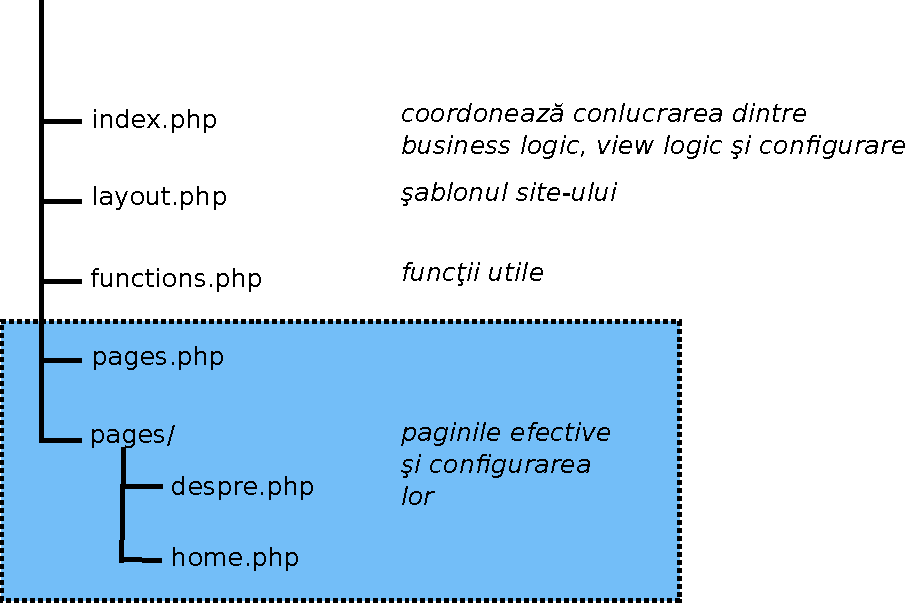
\includegraphics[scale=.5]{cap03/structure-homepage-crop.pdf}
  \caption{Structura fişierelor unui site simplu}
  \label{fig:filestruct-homepage}
\end{figure}

\begin{Exercise}[title={Îmbunătăţeşte-ţi pagina personală},difficulty=1]
\ExePart
Momentan meniul conţine link  si pentru pagina activă,
ceea ce nu prea are sens. Extinde funcţia
\texttt{build\_menu\_from\_pages} astfel încât să
nu genereze link pentru pagina activă momentan, ci
doar să o afişeze în lista neordonată ca text.

\ExePart
\texttt{index.php} conţine \textit{business logic}-ul site-ului tău.
Extinde acest \textit{business logic} astfel încât pentru
paginile inexistente să arate o pagină \texttt{notfound.php}.
\texttt{home.php} trebuie să rămână în continuare pagina de
start standard a site-ului.

\ExePart
Adaugă încă o pagină \textit{Despre tine}
care afişează informaţii despre vizitator din array-ul superglobal
\texttt{\$\_SERVER}.

Dacă ştii CSS, stilizează site-ul aşa încât să fie mai aspectuos.
Nu va trebui să modifici în nici un fel layout-ul sau
paginile individuale. Vei lucra doar cu CSS.
%TODO wiki: posibilă greşeală: folosirea $_SERVER direct în view
\end{Exercise}

Din partea I a exerciţiului se observă în practică un alt avantaj
al funcţiilor: nu trebuie să editezi multe fişiere în lungul
şi-n latul proiectului, nu te atingi de \textit{business logic}
sau de \textit{view logic} deoarece nu modifici modul fundamental de funcţionare
al acestora. Doar îmbunătăţeşti funcţia, iar
modificările sunt preluate automat în toate locurile de unde
aceasta este apelată.

\section{Directorul curent de lucru}
Căile relative către fişiere şi directoare,
sunt relative la ceea ce numim \textsl{current working
directory}. La \textsl{runtime} (în timpul execuţiei
scriptului), putem afla CWD-ul cu
funcţia \texttt{getcwd()}, şi schimba CWD-ul cu \texttt{chdir()}.

În exemplele anterioare, instrucţiuni precum
\begin{lstlisting}
<?php
require_once 'functions.php';
\end{lstlisting}
au funcţionat deoarece directorul curent de lucru \texttt{'.'}
este specificat în mod standard în directiva \texttt{php.ini}
\texttt{include\_path}. Modul corect de a include un fişier, fără
a ne baza pe faptul că acesta se află în \texttt{include\_path}, ar fi
\begin{lstlisting}
<?php
require_once './functions.php';
\end{lstlisting}
unde \texttt{'.'} se referă la CWD.

Dacă avem însă un scenariu mai complex, cu următoarele fişiere:
\begin{figure}[h!]
  \centering
    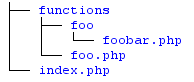
\includegraphics[scale=.7]{cap03/cwdtree.png}
  \caption{Scenariu includere}
  \label{fig:cwdtree}
\end{figure}

\begin{lstlisting}[title=index.php]
<?php
require_once './functions/foo.php';

echo 'index.php este in directorul ',__DIR__,PHP_EOL;

echo 'apelul la foo() genereaza:';
foo();
echo PHP_EOL;
\end{lstlisting}

\begin{lstlisting}[title=functions/foo.php]
<?php
require_once './foo/foobar.php';
function foo() {
        echo __DIR__;
}
\end{lstlisting}

\begin{lstlisting}[title=functions/foo/foobar.php]
<?php
function foobar() {
}
\end{lstlisting}

atunci toate fişierele sunt incluse prin prisma fişierului
\texttt{index.php}, deci CWD-ul este directorul
în care se află acest fişier. Asta nu este
o problemă pentru linia 2 din \texttt{index.php},
deoarece directorul \texttt{'.'} coincide
cu directorul în care se află \texttt{index.php}.

Însă devine o problemă atunci când din fişierul
inclus \texttt{foo.php} vrem să includem
un alt fişier dintr-un alt subdirector
\texttt{functions/foo/}, deoarece CWD-ul nu se
schimbă, şi deci, relativ la directorul
în care se află \texttt{index.php}, nu există
un subdirector \texttt{./foo/foobar.php}.

O metodă foarte elegantă la problema asta este să definim
o constantă în \texttt{index.php}, constantă care
va fi folosită la includerea fişierelor. Astfel am
avea:

\begin{lstlisting}[title=index.php]
<?php
const APP_ROOT = __DIR__;
require_once APP_ROOT . '/functions/foo.php';

echo 'index.php este in directorul ',__DIR__,PHP_EOL;

echo 'apelul la foo() genereaza:';
foo();
echo PHP_EOL;
\end{lstlisting}

\begin{lstlisting}[title=functions/foo.php]
<?php
require_once APP_ROOT . '/functions/foo/foobar.php';
function foo() {
        echo __DIR__;
}
\end{lstlisting}
Cu această tehnică vom avea în lungul şi-n latul
aplicaţiei constanta \texttt{APP\_ROOT} care
conţine mereu calea către directorul în
care se află în \texttt{index.php}, indiferent
de fişierul prin care trece momentan fluxul
de execuţie.

Cu adevărat flexibilă devine această metodă
atunci când avem aplicaţii multiple care
folosesc un set comun de funcţii. Nu va trebui
să copiem fişierele de colo colo, ci vom
dezvolta doar o singură "versiune" a acestor
funcţii comune, definind o constantă 
de genul \texttt{APP\_LIB} cu calea către
directorul ce conţine fişiere PHP
cu implementările funcţiilor noastre. Din a doua aplicaţie
care doreşte să folosească funcţiile primei
aplicaţii, nu trebuie decât să definim
\texttt{APP\_LIB} ca calea către
directorul cu funcţii din prima aplicaţie,
cea "originală".

Şi mai curat din punct de vedere organizatoric
este să punem toate aceste funcţii într-o
locaţie neutră, astfel încât să nu aparţină
nici unui proiect, şi din toate
proiectele să definim calea către acea
locaţie.

O altă tehnică implică folosirea tocmai
a acestei constante magice  \texttt{\_\_DIR\_\_}.

Cu această tehnică nu mai e nevoie
să definim constante "globale" precum \texttt{APP\_ROOT},
însă nici nu mai putem reutiliza porţiuni
de funcţionalitate în lungul şi-n latul
diferitelor proiecte independente unul de celălalt.

Un astfel de cod ar arăta astfel:
\begin{lstlisting}[title=index.php]
<?php
require_once './functions/foo.php';
foo();
\end{lstlisting}

\begin{lstlisting}[title=functions/foo.php]
<?php
require_once __DIR__ . '/foo/foobar.php';
function foo() {
}
\end{lstlisting}

\begin{lstlisting}[title=functions/foo/foobar.php]
<?php
function foobar() {
}
\end{lstlisting}

\good{Includerea fişierelor ar trebui să o faci mereu folosind
căi absolute, precum o constantă globală aplicaţiei sau cu
constanta magică \texttt{\_\_DIR\_\_}.

Atunci când foloseşti căi absolute, PHP nu trebuie să ia
la rând căile din \texttt{include\_path}, ceea ce îl absolvă
pe PHP de multe accese ale hard-disk-ului - aceste accese
fiind destul de costisitoare.}

\section{Formulare II. File uploads}
Cu PHP, poţi oferi utilizatorului posibilitatea de a salva fişierele
proprii pe hard disk-ul serverului. Este ceea ce numim \textsl{file upload}.

Formularele care conţin câmpuri pentru upload trebuie să fie trimise
cu metoda HTTP POST, şi să fie codate ca \texttt{multipart/form-data}.

Un exemplu:
\begin{lstlisting}[title=index.php]
<?php
require_once __DIR__ . '/functions.php';

echo '<pre>';
var_dump($_FILES);
echo '</pre>';
?>
<form enctype="multipart/form-data" method="POST">
<input type="hidden" name="MAX_FILE_SIZE"
	value="<?php echo return_bytes(ini_get('upload_max_filesize'));?>" />
<input name="myfile" type="file" />
<input type="submit" value="Send" />
</form>
\end{lstlisting}

\begin{lstlisting}[title=functions.php]
<?php
function return_bytes($val) {
  $val = trim($val);
  $last = $val[strlen($val)-1];
  switch($last) {
	case 'g':
	case 'G':
	  $val *= 1024;
	case 'm':
	case 'M':
	  $val *= 1024;
	case 'k':
	case 'K':
	  $val *= 1024;
  }
  return $val;
}
\end{lstlisting}
Codul este destul de sugestiv. La primirea fişierelor (cu succes sau cu erori, nu
contează), informaţiile\footnote{metadatele} despre ele vor fi disponibile
în array-ul superglobal \texttt{\$\_FILES}.

Elementul \texttt{'error'} din fiecare set de metadate va conţine
codurile de eroare pe care le poţi compara
cu constantele specifice\footnote{\url{http://www.php.net/manual/en/features.file-upload.errors.php}}
pentru a determina cauza erorii.

\good{Este recomandat să foloseşti aceste constante predefinite, precum
\texttt{UPLOAD\_ERR\_OK}, în loc de valorile numerice concrete, pentru
o mai bună portabilitate.}

Elementul \texttt{tmp\_name} este calea absolută către fişierul efectiv.
Atunci când utilizatorul uploadează un fişier, acesta primeşte un nume
temporar aleatoriu, şi este salvat acolo unde specifică
directiva de configurare \texttt{php.ini} \texttt{upload\_tmp\_dir}.

Numele real al fişierului, aşa cum a fost uploadat de utilizator,
se află în \texttt{'name'}.

\texttt{'type'} este tipul MIME al documentului.

Alte directive care influenţează upload-ul de fişiere sunt
\begin{itemize}
\item \texttt{post\_max\_size} pentru mărimea totală a datelor trimise prin POST, mărime care include
	  cumulativ mărimea tuturor datelor trimise, nu numai a fişierelor
\item \texttt{max\_input\_time} limitează timpul pe care PHP are voie să îl petreacă
  procesând datele trimise. Acest timp depinde în mare măsură de rata de upload
  a clientului şi de rata de download a serverului
\item \texttt{file\_uploads} poate activa sau dezactiva uploadul de fişiere dintr-un foc
\item \texttt{max\_file\_uploads} limitează numărul de fişiere ce pot fi uploadate de
  client într-o singură cerere HTTP
\end{itemize}

Din moment ce fişierul uploadat se află într-un director ce nu aparţine
aplicaţiei noastre, cu un nume aleatoriu, va trebui să
îl mutăm în interiorul aplicaţiei noastre. Pentru
a verifica dacă un fişier este un fişier uploadat folosim
\texttt{is\_uploaded\_file()}, iar pentru a muta
acel fişier, folosim \texttt{move\_uploaded\_file()}.


\good{Deschide manualul PHP şi documentează-te despre aceste funcţii.
Manualul conţine exemple de utilizare şi o mulţime de comentarii
din partea altor utilizatori din care cu siguranţă poţi
învăţa câte ceva.}

\begin{Exercise}[title={Remote file storage},difficulty=2]
\ExePart

Crează o aplicaţie care permite utilizatorilor să
uploadeze fişiere pe serverul tău.

Utilizatorii vor trebui să introducă şi un nume secret
care va fi folosit de aplicaţie pentru crearea unui subdirector
corespunzător, director în care va fi pus fişierul uploadat.

Fişierele uploadate se vor afla deci în directorul
\texttt{uploads/<nume secret>/}. Astfel, utilizatori
care se cunosc între ei vor putea uploada colaborativ
fişiere, lucrând cu un \texttt{<nume secret>} comun.

Foloseşte funcţii ca \texttt{is\_dir()} şi
\texttt{mkdir()}. Explorează manualul dacă te
loveşti de necesitatea folosirii altor funcţii.

Nu uita să verifici toate erorile posibile şi
imposibile, şi că aplicaţia trebuie să
se comporte normal şi să genereze cod \textit{XHTML 1.1} valid, chiar şi atunci
când aplicaţia ta generează erori.

Nu uita nici de separarea \textit{business logic}-ului
de \textit{view logic}. Construieşte-ţi aplicaţia
cât mai modularizat posibil.

\ExePart
Ce găuri de securitate identifici?
% dacă numele există deja, userul \^işi poate da seama de asta
\end{Exercise}

\section{Lucrul cu fişiere}
Până acum am lucrat cu fişiere ca entităţi opace, fără
a citi din sau a scrie în ele.

PHP pune la dispoziţie funcţii pentru lucrul
cu fişiere. Aşa cum în paginile trecute am deschis un
director pentru a-l itera, şi apoi l-am închis, eliberându-l,
tot la fel putem lucra şi cu informaţiile salvate în fişiere.

Pentru a opera pe un fişier, trebuie să îl deschidem cu
\texttt{fopen()}. Ne alegem cu un \textsl{file handler}
care va fi pasat ca parametru funcţiilor următoare
de manipulare a fişierelor.

Deschiderea fişierelor se face în moduri precum "citire",
"scriere" sau "adăugare". O listă completă ale acestor
moduri se găseşte pe pagina \texttt{fopen()} din manualul
PHP.

Atunci când deschidem fişierul, dispunem de un cursor\footnote{Numit şi
\textit{file pointer} în manualul PHP.}
pe care îl putem plimba în lungul şi-n latul fişierului.
În funcţie de modul în care am deschis fişierul, acest
cursor se va afla imediat după deschiderea
fişierului cu \texttt{fopen()} fie la începutul, fie la sfârşitul
fişierului. În modul \textit{read}, cursorul se va
afla la început. În modul \textit{append}, la sfârşit.

Citirea din fişier o facem cu \textsl{fread()}, funcţie căreia trebuie
să-i spunem şi ce lungime maximă în bytes vrem să aibă segmentul
de informaţie citit.
La apelarea acestei funcţii, cursorul va fi înaintat cu numărul
de bytes citiţi.

Deoarece nu ştim ce mărime are fişierul, va trebui să citim
în mod repetat din fişier, într-o buclă, până când ne aflăm
la \engl{sfârşitul fişierului}{end of file}, prescurtat EOF.
Pentru a testa dacă am ajuns la EOF, folosim funcţia \texttt{feof()}.

După ce am terminat de operat pe fişier, trebuie să-l închidem cu
\texttt{fclose()}.

\begin{Exercise}[title={Citeşte din fişier}]
Scrie un program care 
citeşte un număr aleatoriu de bytes între 1 şi 32 dintr-un fişier deja existent
şi afişează stringurile citite la fiecare iteraţie în câte
un bloc HTML \texttt{<pre></pre>}.

Dacă fişierul nu este \textit{readable}, programul trebuie
să arate un mesaj de eroare corespunzător.

Pentru generarea de numere aleatoare foloseşte funcţia
\texttt{rand()} din extensia \textit{Math} a categoriei
de extensii \textit{Mathematical Extensions}.

Citeşte cu atenţie paginile din manual ale funcţiilor pentru
lucrul cu fişiere menţionate mai sus, secţiunile \textit{User
Contributed Notes} şi explorează şi alte posibilităţi
dincolo de ceea ce te interesează pentru rezolvarea acestui
exerciţiu urmând link-urile din secţiunile \textit{See Also}
ale acestor funcţii.
\end{Exercise}

De multe ori vom fi nevoiţi să structurăm informaţiile aflate \^in
fişiere. De exemplu hai să ne imaginăm că vrem să facem un guestbook.

Asta \^inseamnă că utilizatorul intră pe pagina noastră şi completează
c\^ampuri precum \textit{nume} şi conţinut. Teoretic am putea citi
aceste informaţii şi le-am putea adăuga la sf\^arşitul unui fişier
care ar avea funcţia de {\glqq}bază de date{\grqq}. Acest
fişier ar conţine toate impresiile lăsate de toţi vizitatorii noştri.

Dar ce facem dacă vrem să edităm o anumită intrare? Ar trebui să
deschidem \^intregul fişier şi să navigăm p\^ană la intrarea \^in cauză
pentru a o edita. \^in afară de asta, ne-ar fi greu să identificăm
bucata de text pe care o vrem.

Pentru a structura informaţiile dintr-un fişier, e suficient să
introducem o sintaxă nouă. De exemplu, am putea spune că
cele două c\^ampuri de date \textit{nume} şi \textit{text} sunt separate
de caracterul \texttt{|}. {\glqq}Baza noastră de date{\grqq} ar
putea arăta astfel:
\begin{verbatim}
Flavius|Hello world
Florin|Hello back
\end{verbatim}
Ce se \^int\^amplă dacă numele meu este \textsl{Fla|vius}? Caracterul separator
\texttt{|} va trebui escaped şi el.

Din fericire există un format de date deja larg răsp\^andit iar PHP ne
pune la dispoziţie funcţii pentru lucrul cu el. Formatul se numeşte
\textsl{comma-sepparated values} (abv. CSV).
Separatorul acestui format este virgula, iar funcţiile fac escaping automat. Aceste funcţii sunt
\texttt{str\_getcsv()}, \texttt{fgetcsv()}, \texttt{fputcsv()}.

CSV este un format ce se pretează pentru date tabelare. Un alt format este \texttt{INI}. Formatul
unui fişier .ini este
\begin{verbatim}
;this is a comment
[section1]
key1=value1
key2=value2

[section2]
key1=value1
array[]=value2
array[]=value3
\end{verbatim}

După cum putem deduce din exemplu, formatul .ini se pretează pentru perechi de valori,
numite şi dicţionare. Adiţional, aceste perechi pot fi grupate \^in secţiuni.

Pentru lucrul cu acest format avem la dispoziţie funcţiile
\texttt{parse\_ini\_string()} şi \texttt{parse\_ini\_file()}.

Manualul PHP conţine multe exemple şi detalii despre aceste funcţii
şi formate de date.

\subsection{Filesystems}

Un \textsl{filesystem} (abv. FS) este un mod de organizare a fişierelor
şi directoarelor pe \textit{hard disk}. Există nenumărate
astfel de \textit{filesystems}, specifice unor anumite
sisteme de operare, sau create pentru a rezolva anumite tipuri
de probleme. De exemplu, utilizatorii Microsoft Windows folosesc
de obicei \textsl{NTFS}, utilizatorii *NIX \textsl{ext2}, \textsl{ext3}
sau \textsl{ReiserFS}, iar pentru accesarea transparentă a fişierelor
de pe un alt calculator conectat prin reţea de nodul curent se
poate folosi \textsl{NFS} (en. \textsl{Network File System}).

Sub GNU/Linux există însă mai multe tipuri de {\glqq}fişiere{\grqq}:
fişierele normale, directoarele, link-uri simbolice (en. \textsl{symlinks}),
\textsl{device}, \textsl{named pipe} şi \textsl{unix socket}.

Deoarece nu ştim pe ce fel de platformă va rula aplicaţia (scriptul)
nostru, este imperativ să verificăm dacă ceea ce urmează să deschidem
este \^intr-adevăr un fişier sau un director cu \texttt{is\_file()}
şi respectiv \texttt{is\_dir()}.

Unele \textit{filesystems} oferă posibilitatea de a specifica 
un proprietar al unui fişier sau director, sau drepturi de acces.
De aceea este recomandat să foloseşti funcţii precum \texttt{is\_readable()}
sau \texttt{is\_writable()} \^inainte de a deschide fişierele
sau directoarele \^in cauză pentru citire din sau scriere \^in ele.

\^In cazul \^in care creezi programatic fişiere, nu uita că
umask-ul procesului PHP determină drepturile standard de acces
ale fişierului nou creat. Deasemenea nu uita că utilizatorul sub
care rulează parserul PHP va fi proprietarul fişierelor create
programatic.\footnote{De obicei numele utilizatorului din sistem
este {\glqq}nobody{\grqq}, {\glqq}httpd{\grqq} sau {\glqq}http{\grqq}, dar
nu este recomandat să te bazezi pe astfel de standarde nescrise.}
Pentru a schimba sau verifica aceste setări, PHP pune la dispoziţie
funcţii precum \texttt{umask()} şi \texttt{chmod()}.

Pentru a \^iţi testa extensiv aplicaţiile pe diferite platforme
precum MS Windows sau GNU/Linux, \^iţi recomand să foloseşti
programe de virtualizare. O listă de resurse despre acestea
şi despre GNU/Linux este pusă la dispoziţie de comunitatea
{\phpro} prin intermediul articolelor.


%TODO fix colaborativ -> nu există în DEX, cooperativ???
\begin{Exercise}[title={Remote file storage cu editare text on-site},difficulty=1]
Extinde aplicaţia creată la exerciţiul anterior astfel încât
utilizatorii să poată edita fişierele de tip text direct
pe site, cu un textbox.
\end{Exercise}

\section{Cookies, sesiuni, autentificare}
Pentru a \^inţelege cum funcţionează autentificarea, trebuie să
reiterăm lucrurile \^invăţate \^in primul capitol despre HTTP.

Clientul stabileşte o conexiune TCP/IP cu daemonul şi \^ii
trimite o cerere \^in formatul HTTP. Această cerere
este formată din \textit{request line} şi \textit{request headers}.

Daemonul răspunde cu \textit{response headers} şi \textit{response body}.
După ce aceste lucruri au avut loc, conexiunea dintre client şi daemon
este \^inchisă. Din acest motiv, spunem că HTTP este un protocol \textsl{stateless}.

Clientul vine şi pleacă după cum pofteşte, se conectează, \^işi ia datele,
şi apoi pierdem legătura cu el. Putem \^insă să \^ii trimitem nişte informaţii {\glqq}speciale{\grqq}
pe care un client (un browser) cooperativ ar trebui să le salveze pe hard disk-ul
utilizatorului şi să ni le trimită iar atunci c\^and se conectează ulterior
la noi şi ne cere ceva. Aceste bucăţi de informaţii se numesc \textsl{cookies}.

Mărimea maximă a unui cookie este de 4 kb \^in aproape toate browserele moderne şi
des \^int\^alnite, iar numărul de cookies pe care un domeniu are voie să
le seteze variază de la browser la browser. \^In trecut limita era de
20, dar chiar şi asta este mult pentru o aplicaţie tipică,
modernă, scrisă \^in PHP,
unde de obicei un singur cookie este suficient.

Deci hai să ne jucăm cu cookies:

\begin{lstlisting}[title=Folosirea cookie-urilor]
<?php
setcookie('random',rand(100,999));
var_dump($_COOKIE);
\end{lstlisting}

Linia 2 setează un cookie numit {\glqq}random{\grqq}.
Vom crea o cerere HTTP cu telnet pe portul 80:
\begin{verbatim}
GET /cookie.php HTTP/1.1
Host: localhost

\end{verbatim}

Să zicem că noi, folosind telnet, suntem un browser care cooperează urm\^and
exact ceea ce ne spune daemonul să facem.
Dacă \^in exemplul de mai sus am primit ca răspuns
\begin{verbatim}
Set-Cookie: random=139
\end{verbatim}
atunci, la vizita următoare, \^ii vom pasa acest cookie daemonului,
cu valoarea pe care ne-a transmis-o.

Deci trimitem cererea:
\begin{verbatim}
GET /cookie.php HTTP/1.1
Host: localhost
Cookie: random=139

\end{verbatim} 
Şi primim răspunsul
\begin{verbatim}
HTTP/1.1 200 OK
Date: Thu, 21 Oct 2010 13:20:17 GMT
Set-Cookie: random=278

array(1) {
  ["random"]=>
  string(3) "139"
}
\end{verbatim} 

Cookie-ul numit 'random' are acum altă valoare, 278, aşa cum este generat de linia 2 din script. \^Insă
array-ul superglobal \texttt{\$\_COOKIE} nu conţine acea nouă valoare generată şi trimisă
clientului. \texttt{\$\_COOKIE} conţine doar ceea ce a fost trimis de client.

\attention{Din aceasta deducem că \texttt{\$\_COOKIE} conţine tot input, şi
ca orice input, trebuie verificat, filtrat şi sanitizat.}

Al treilea parametru al funcţiei \texttt{setcookie()} este \textsl{timestamp}-ul p\^ană
c\^and va fi valabil acel cookie. Dacă nu e specificat, un browser poate
şterge acel cookie de \^indată ce este \^inchis. 

Timestamp reprezintă numărul de secunde care au trecut de la 1 ianuarie 1970. Se mai numeşte
şi UNIX timestamp. Numărul de secunde se calculează \^in fusul orar GMT.\footnote{Deoarece
are decalaj 0} Pentru a şterge un cookie, pur şi simplu setăm data expirării \^in trecut.

Pentru restul parametrilor ar trebui să consulţi manualul PHP. Dacă ai \^intrebări
despre folosirea cookie-urilor, comunitatea {\phpro} \^iţi stă la dispoziţie.

Cookie-urile sunt utile atunci c\^and vrei să salvezi preferinţele vizitatorului
pe site. De exemplu indiciile vizuale precum limba preferată \^in care ar
trebui afişat site-ul sau care meniuri sunt vizibile şi care nu.

Cookie-urile nu ar trebui folosite pentru salvarea datelor sensibile sau personale
precum username, parolă, sau orice alte date care nu vrei să fie setate aleatoriu
de client. Pentru că nu uita, aceste informaţii sunt lucruri pe care
clientul le poate scrie după buna sa plăcere, aşa cum am făcut-o noi cu telnet.

Pentru a salva informaţii compozite\footnote{adică array-uri} \^in cookies
poţi serializa
şi deserializa informaţiile folosind diferite formate, fie inventate de tine,
fie puse la dispoziţie de PHP:
\begin{itemize}
 \item nativ PHP: \texttt{serialize()} şi \texttt{unserialize()}
 \item URL-encoded: \texttt{http\_build\_query()} şi \texttt{parse\_str()}
 \item JSON: \texttt{json\_encode()} şi \texttt{json\_decode()}
\end{itemize}


\subsection{Sessions}
O formă {\glqq}specială{\grqq} de cookie este aşa numita \textsl{session cookie}.
O session cookie nu conţine informaţii preţioase pentru un eventual atacator,
ci un simplu ID unic. Numele cookie-ului care va conţine ID-ul poate fi
obţinut sau setat cu \texttt{session\_name()}.

Informaţia salvată \^in acest cookie, adică ID-ul, poate fi obţinut cu
\texttt{session\_id()}.

\^Inainte de a lucra totuşi cu sesiuni, trebuie să apelăm \texttt{session\_start()}.
Deoarece pornirea subsistemului PHP pentru sesiuni implică adăugarea unui header
'Set-Cookie', apelul la această funcţie trebuie făcut \^inainte de a scrie orice
\^in \textit{response body}. Căci dacă am scris ceva \^in response body (de exemplu
cu \texttt{echo}), atunci \textit{response header}-ele sunt deja trimise, deci
e prea târziu să mai trimitem un cookie clientului.

Asta ne spune şi eroarea din acest script:
\begin{lstlisting}[title=Headers already sent]
<?php
echo 'hello world';
session_start();
\end{lstlisting}
şi anume
\begin{verbatim}
Warning: session_start(): Cannot send session cookie - headers already sent
\end{verbatim} 

După ce am pornit sesiunea, putem salva informaţii \^in array-ul superglobal
\texttt{\$\_SESSION}. Dar dacă informaţiile nu vor fi salvate \^in cookie-ul
cu numele \texttt{session\_name()}, atunci unde vor fi salvate? Răspunsul:
\^in fişiere. Directiva php.ini \texttt{session.save\_path} ne spune unde se află
aceste fişiere. Fişierele vor fi numite după ID-ul sesiunii. Hai să vedem practic
cum funcţionează acest mecanism:
\begin{lstlisting}[title=Understanding Sessions]
<?php
session_start();
$_SESSION['username'] = 'flav';
echo 'Datele salvate in $_SESSION se afla in fisierul: '.session_save_path().'/sess_'.session_id();
\end{lstlisting}

Deschiz\^and fişierul \^in care ne spune acest script că avem datele, vedem:
\begin{verbatim}
username|s:4:"flav";
\end{verbatim}
Ceea ce vedem aici sunt datele salvate \^in \texttt{\$\_SESSION}, numai că
sunt serializate \^in formatul specific modulului \textit{session}. Conceptul
de \textsl{serializare} \^insuşi l-am cunoscut deja prin formatul json sau funcţii
precum \texttt{serialize()} menţionate anterior.

Funcţia \texttt{session\_start()} nu face nimic altceva dec\^at să citească id-ul
din cookie-ul cu numele returnat de \texttt{session\_name()}\footnote{Care \^in mod
standard este 'PHPSESSID'.}, şi să deserializeze informaţiile aflate \^in fişierul
\texttt{session\_save\_path().'/sess\_'.session\_id()}
şi să le salveze \^in
array-ul superglobal \texttt{\$\_SESSION}.

\subsection{Authentication}
A autentifica pe cineva nu înseamnă nimic mai mult decât a asocia
un identificator unic (un ID) cu un client (un browser), ID
care va fi salvat în două locuri: într-un cookie pe client, şi pe
server, de obicei în numele fişierului din interiorul directorului
\texttt{session\_save\_path()}.

Deşi repet, ţin să subliniez încă o dată cât de \textit{fragilă} este această
autentificare: un simplu string de câteva zeci de caractere
(session ID) face diferenţa dintre a fi autentificat sau nu ... sau
a fi autentificat ca altcineva.

Dacă cineva reuşeşte să facă rost de ID-ul unei sesiuni al unui
alt utilizator, e ca şi autentificat ca acel utilizator.

Ţi-ai putea imagina că a face rost de acest ID este ceva destul de
complicat, şi că nu "oricine" ar putea face asta. Din fericire\footnote{"din
fericire" deoarece este încă un motiv în plus să acordăm o atenţie
deosebită securităţii aplicaţiilor noastre} pentru noi, acest lucru este
relativ trivial  -- în capitolul 5 vei vedea cum o singură greşeală
banală îi poate oferi atacatorului site-ului tău să injecteze cod HTML
şi Javascript care să îi trimită acest ID\footnote{Atacul se numeşte
XSS - cross-site scripting}.

Pentru a face lucrurile mai dificile, o măsură adiţională ar putea
fi identificarea şi după adresa IP (\texttt{\$\_SERVER['REMOTE\_ADDR']}),
însă acest lucru are un dezavantaj: dacă îţi aduci bine aminte din
capitolul \textit{Reţelistică}, mai mulţi utilizatori care "împart"
accesul la Internet printr-un router au aceeaşi adresă IP publică.

Făcând autentificarea şi\footnote{nu "doar", ci "şi", conjunctiv: atât
după sesiune, cât şi după IP} după adresa IP, aplicaţia ta ar putea
deveni "confuză" deoarece vede o singură adresă IP şi mai multe
ID-uri de sesiune.

Adresa IP şi ID-ul unic din cookie nu sunt însă singurele elemente
ce pot fi luate în considerare la autentificarea unui utilizator.
Majoritatea browserelor, numite şi \textsl{agenţi}, trimit un string
la fiecare cerere, pe care îl poţi accesa prin \texttt{\$\_SERVER['HTTP\_USER\_AGENT']}.

\begin{Exercise}[title={O schemă de autentificare ieşită din comun},difficulty=2]
Extinde {\glqq}remote file storage{\grqq} cu autentificare.
Parola va fi acel {\glqq}<nume secret>{\grqq}, iar fiecare {\glqq}nume
secret{\grqq} va avea un fişier \texttt{uploads/<nume secret>/users.csv}
ce va conţine o listă de usernames. La crearea unui nou \texttt{<nume secret>},
proces numit "înregistrare" pe site-urile pe care le cunoşti deja,
userul va trebui să uploadeze acel fişier \texttt{users.csv}. Nu vor exista
drepturi de acces, deci toată lumea va putea interzice accesul tuturor celorlalţi
de \^indată ce are credentials \^in \texttt{users.csv}.
\end{Exercise}

\begin{Exercise}[title={Remote file storage cu galerie de imagini}]
Extinde aplicaţia de la exerciţiul anterior astfel încât să detecteze
dacă un {\glqq}<nume secret>{\grqq} are doar imagini în el, şi dacă
da, să afişeze acel director ca pe o galerie de imagini.
\end{Exercise}

\begin{Exercise}[title={Guestbook I},difficulty=2]
Crează un guestbook simplu, cu autentificarea unui singur
administrator. Intrările din guestbook trebuiesc salvate (serializate)
într-un format la alegere (json, csv sau un format propriu), dar
nu trebuie să fie HTML.

Utilizatorii care vor să lase un mesaj vor introduce nume, adresă e-mail, un 
URL opţional şi mesajul care poate conţine doar tagurile HTML:
\texttt{<b>}, \texttt{<i>}, \texttt{<p>}.

Adiţional, o linie goală poate delimita paragrafe.

Crează şi o interfaţă de administrare, sistemul va avea un singur utilizator:
administratorul. Prin interfaţa de administrare acesta va putea şterge sau edita
intrările din guestbook sau bana adrese IP.
\end{Exercise}

\section{Felicitări}
În aceste capitole ai învăţat să lucrezi cu conceptele fundamentale
din programare. Pe baza noţiunilor de reţelistică ai putut înţelege
diferiţi vectori de atac, cum să îţi protejezi aplicaţiile împotriva
lor, cum poţi autentifica şi autoriza utilizatorii, şi multe
alte posibilităţi prin intermediul funcţiilor puse la dispoziţie de
PHP.

Ai învăţat şi cum îţi poţi modulariza codul astfel încât componente
precum \textit{business logic}, \textit{view logic} sau configurarea să fie
reutilizabile, eventual pe baza unor funcţii proprii, care ar
trebui să fie la rândul lor la fel de reutilizabile.

Pentru a concepe toate aceste lucruri, ai învăţat şi cum să inventezi
structuri de date abstracte, pe care toate aceste
lucruri\footnote{business logic, view logic, funcţiile PHP şi
funcţiile proprii} pot opera colectiv.

\begin{Exercise}[title={Recapitulare şi sinteză}]
Citeşte cu atenţie sinteza de mai sus, apoi închide cartea şi scrie o
sinteză mai detaliată despre ce ai învăţat în propriile cuvinte,
de cel puţin 300 de cuvinte.

Mult mai importantă dec\^at corectitudinea tehnică a rezumatului
este capacitatea ta de a jongla cu noţiunile, chiar şi cu
riscul de a greşi, deci nu te sfii a face afirmaţii \^indrăzneţe.
\end{Exercise}


%php baze de date, mysql, lucrul în echipă
\chapter{Baze de date şi lucrul în echipă}
\vskip -25pt
\textit{În acest capitol vei învăţa fundamentele bazelor de date şi lucrul într-o echipă de programatori,
cu toate uneltele necesare şi unele \textit{soft skills} de care are nevoie un programator.
\vskip 1em
Scopul acestui capitol este să te pregătească pentru exerciţiul de la sfârşitul capitolului
care constă într-un proiect pe care îl vei face într-o echipă.
Începând cu acest capitol, tutorii {\phpro} mai mult te vor îndruma, te vor consilia, atât
pe tine individual, doar atunci când ai absolut nevoie, dar mai ales pe întreaga echipă.
\vskip 1em
Prin urmare, vei fi mult mai independent, dar vei şi avea o responsabilitate mai mare --
cel puţin faţă de colegii de echipă.
}
\vskip 5em

\section{Git}
\subsection{Istoria unui proiect}
Probabil că până acum te-ai confruntat deja cu următorul scenariu: vrei
să testezi ceva în programul tău, dar nu eşti sigur că schimbarea
va deveni permanentă.

Cel mai probabil te-ai folosit de comentarii în astfel de cazuri: ai comentat
o parte din codul sursă şi ai scris o nouă implementaţie dedesubt. Dacă a
fost vorba de modificări prin mai multe fişiere, probabil ai repetat acelaşi
procedeu pentru fiecare dintre acestea.

Dacă ai avut noroc, schimbările tale au fost bune, şi tot ce a trebuit să
faci în cele din urmă a fost să ştergi implementaţia veche, comentată,
şi să o laşi doar pe cea nouă în loc.

Dacă nu ai avut noroc, ţi-ai dat seama că ideea ta nu a fost cea mai grozavă,
şi a trebuit să restaurezi versiunea veche. În urma restaurării, probabil ai
avut noroc şi ai reuşit să revii la versiunea veche fără probleme.

Însă cel mai probabil, nu ai avut noroc deloc.

Ei bine, mulţumită unor programe numite \textsl{revision control systems}
(abv. RCS),
nu ai nevoie de noroc atunci când codul sursă al proiectului tău evoluează,
sau când doar vrei să testezi lucruri noi.

Cu un RCS, nu mai e nevoie să laşi la voia întâmplării modificările
aduse codului -- tot ceea ce faci este înregistrat, fiecare schimbare,
fie ea şi cât de mică. Partea bună e că poţi reveni la orice versiune
a codului, oricând, oricum!

Deşi ai multe avantaje atunci când foloseşti un RCS ca un programator singur,
RCS-urile îşi dezvoltă adevărata putere atunci când lucrezi în echipă
cu alţi programatori.

Printre cele mai cunoscute RCS-uri se numără \textit{subversion},
\textit{mercurial}, \textit{bazaar}, \textit{BitKeeper} şi \textit{git}.

În acest curs, vei folosi Git. Git s-a născut din necesitatea
programatorilor kernelului Linux de a-şi controla mai organizat
procesul de dezvoltare.

Spre deosebire de subversion, cu git nu există un server central,
de aceea git se numeşte şi DRCS, D venind de la \textsl{distributed}.

Pentru o listă a termenilor cei mai importanţi citeşte despre
\href{http://en.wikipedia.org/wiki/Revision_control}{revision control}.

\subsection{Getting started}
Sub GNU/Linux, instalarea este destul de simplă: foloseşte
package manager-ul distribuţiei tale pentru a instala pachetul "git".

Pentru Microsoft Windows,
intră pe pagina oficială\footnote{\url{http://code.google.com/p/msysgit/}}
şi instalează \textit{Full installer for official Git}. La pasul
\textit{Adjusting your PATH environment}, selectează \textit{Run
Git from the windows command prompt}. Restul opţiunilor ar trebui
să fie bune aşa cum ţi le prezintă installer-ul. Pe desktop ar trebui
să-ţi apară simbolul "git bash".

După ce ai instalat git, urmează cartea ProGit\footnote{\url{http://progit.org}},
capitolele 1-3. Aceasta îţi va prezenta mai toate noţiunile elementare
despre git.

\begin{Exercise}[title={A taste of git}]
Dacă eşti în programul de tutelare, ai deja cont pe github.com.
Acest site îţi oferă hosting pentru proiectele tale. Intră
în contact cu noi pe IRC pentru a fi îndrumat.

Crează un nou proiect pe github.com denumit la fel ca username-ul
tău de pe github.com, iar apoi clonează-l local şi experimentează
cu el.

Pentru lucrul cu repozitoriile hostate pe github, citeşte instrucţiunile
de configurare de pe github\footnote{\url{http://help.github.com/}}.

Întreabă-i pe ceilalţi cursanţi ce lucruri interesante mai poţi face
cu git.

Încearcă să te joci cât mai mult cu acest utilitar, deoarece de acum
încolo toate proiectele tale vor fi puse sub revision control în git.

Îţi aminteşti probabil şi de "gist-ul" unde ţi-ai salvat toate soluţiile
la exerciţii până acum. Ei bine, un "gist" nu este nimic altceva decât
un repozitoriu git. Îl poţi clona bine mersi, şi opera pe el
din confortul consolei tale -- nu e nevoie să accesezi interfaţa
web pentru a posta ceva.

Crează un fork al cărţii, fă mici corecturi acolo unde vezi necesar,
dacă ai găsit greşeli în carte, învaţă să faci pull
requests, să trimiţi patchuri, să deschizi issues pe interfaţa web
a proiectelor tale pusă la dispoziţie de github.

Investeşte în jur de 40-80 de ore de lectură şi de experimente pentru
a deveni cât de cât rutinat în folosirea acestor sisteme: git
ca utilitar de sine stătător pe de o parte, şi github.com ca
hosting pentru proiectele tale.
\end{Exercise}

\section{Baze de date relaţionale}
Bazele de date sunt folosite pentru a salva informaţii structurate.
După structura datelor, există două cele mai răspândite forme de
baze de date:
\begin{itemize}
\item relaţionale
\item orientate pe obiecte
\end{itemize}
Bazele de date relaţionale (abv. \textsl{RDBMS}) se pretează pentru informaţii "tabelare"
ce pot avea relaţii între ele. Cele orientate pe obiecte se pretează
pentru informaţii arborescente -- gândeşte-te la arborescenţa
(şi recursivitatea) unui document HTML.



În funcţie de modul de acces, pentru ambele tipuri de mai sus există
iarăşi două categorii:
\begin{itemize}
\item de sine stătătoare
\item după arhitectura server-client
\end{itemize}

Pentru a folosi o bază de date de sine stătătoare nu ai nevoie de un
server. Baza de date constă într-un fişier care conţine toate datele
şi metadatele. Aceste baze de date pot fi trimise uşor altcuiva
şi nu este nevoie decât de un program care ştie să opereze pe acea
bază de date. Un exemplu consacrat pentru astfel de baze de date
este SQLite.

Bazele de date cu server-client au în mare trei componente:
\begin{itemize}
\item fişierul\footnote{în funcţie de RDBMS şi de alţi
factori, pot fi mai multe fişiere} efectiv în care sunt salvate
informaţiile
\item daemonul care aşteaptă conexiuni de pe internet şi
deserveşte informaţii din acele fişiere
\item clientul care se conectează la server şi cere informaţii
\end{itemize}

Atunci când clientul cere informaţii de la un server, clientul
nu primeşte toate informaţiile, pentru a-şi putea alege ce vrea.
Clientul trimite o cerere într-un limbaj special, cerere pe baza
căreia serverul generează un răspuns care conţine deja informaţiile
dorite de client.

Deşi nu este relevant pentru folosirea bazelor de date, e important
să clarificăm cum funcţionează aceste componente, şi vom încerca
să o facem pe baza cunoştinţelor pe care le avem deja despre
protocolul HTTP şi programele care îl folosesc.

Clientul DB se conectează la serverul DB printr-un protocol
de transfer al informaţiilor precum TCP/IP, similar cu
felul în care şi un browser se conectează la un daemon HTTP.

Transferul de informaţii efectiv se face într-un limbaj înţeles
de aceste două programe -- un protocol -- din nou: analog cu HTTP.

Una dintre diferenţele cruciale este însă că acest client nu se
conectează, trimite o cerere, primeşte un răspuns, şi apoi se
deconectează. Nu. Acest lucru se întâmplă în cazul protocoalelor
\textit{stateless} precum HTTP. DBMS-urile în schimb au de obicei
protocoale \textsl{stateful}, adică se conectează la daemon, şi
aceasta este menţinută până la întreruperea ei explicită.

Odată conectat, clientul e pregătit să trimită cereri formulate
într-un limbaj specific. În cazul RDBMS-urilor, predominant este
limbajul SQL (en. \textsl{Structural Query Language}
, citit \texttt{\textipa{si:kw@l}}).% IPA: siːkwəl

Această cerere formulată în limbajul SQL este apoi codată în
protocolul specific DBMS-ului şi trimisă acestuia.
Faptul că fiecare\footnote{aproape fiecare} DBMS are un protocol
specific este cauza imposibilităţii comunicării cu un daemon
de un tip folosind un client de alt tip\footnote{De exemplu,
clientul mysql.exe nu poate comunica cu un daemon postgresql.}
-- în ciuda faptului că limbajul în care e formulată cererea, SQL,
este acelaşi\footnote{Există şi aici diferenţe între sisteme,
dar limbajul în sinea lui este acelaşi, este standardizat.}.

În acest capitol vei folosi RDBMS-ul MySQL, deoarece este
cel mai des folosit în conjuncţie cu PHP.

\begin{Exercise}[title={Primii paşi în baze de date}]
\ExePart

Instalează-ţi daemonul şi clientul MySQL. Sub Microsoft
Windows poţi descărca installerul de pe site-ul
oficial\footnote{Se numeşte \textit{MySQL Community Server} şi se găseşte
la adresa \url{http://dev.mysql.com/}.}.

\ExePart

Operaţiile de bază se numesc \textit{create}, \textit{retrieve},
\textit{update}, \textit{delete}, de aici acronimul \textsl{CRUD}.

Accesează manualul MySQL\footnote{\url{http://dev.mysql.com/doc/}}
şi urmează capitolul \textit{Tutorial}. Sub Windows te vei conecta la daemon
cu clientul \texttt{mysql.exe}.

Rezervă-ţi 40-80 de ore de lucru pentru a învăţa să faci operaţii CRUD.
\end{Exercise}

\section{Comunicarea cu MySQL din runtime-ul PHP}
În loc de clientul \texttt{mysql.exe} putem folosi PHP în
calitate de client mysql. 

Desigur, PHP nu ştie de unul singur cum să comunice cu daemonul mysql,
pentru asta fiind nevoie de un modul, o extensie PHP.
Verifică dacă ai modulul \texttt{mysqli} instalat cu comanda:
\begin{verbatim}
php -m
\end{verbatim}
Sub MS Windows, poţi găsi această extensie pe site-ul PECL\footnote{\url{http://windows.php.net/download/} says "PECL extensions for Windows is being worked on."
%TODO check this periodically
}.

\lstinputlisting[label=lst:mysqli connect,caption={Conectarea
la MySQL}]{cap04/1-mysqli-connect.php}

Codul este destul de expresiv. Pe linia 2 obţinem o conexiune.
Pe linia 4, formulăm cererea SQL şi o trimitem conexiunii create.
Având rezultatul, îl putem citi pe tot într-un array bidimensional
cu funcţia \texttt{mysqli\_fetch\_all()} sau l-am putea citi într-o
buclă cu \texttt{mysqli\_fetch\_array()}, ceea ce ar consuma
mai puţină memorie, dar mai mult timp de procesare.

Într-un final, închidem conexiunea creată. Am fi putut totuşi să
trimitem mai multe cereri cu \texttt{mysqli\_query()} dacă am fi
avut nevoie.

Cererea SQL efectivă trimisă ţine de MySQL. Numele funcţiilor,
parametrii şi ordinea lor, cât şi tipurile de date returnate de
acestea ţin de extensia mysqli pe care ai activat-o în \texttt{php.ini}.

Dacă explorezi manualul pentru aceste funcţii, vei vedea că au
două variante, una \textit{object-oriented style} şi una
\textit{procedural style}. Noi vom folosi doar interfaţa procedurală
deocamdată, urmând ca într-un
%TODO spune care
capitol viitor să vedem cum funcţionează şi cea obiectuală.

Deşi funcţiile precum \texttt{mysqli\_connect()} returnează obiecte,
gândeşte-te deocamdată la ele ca la tipuri de date opace.
Atunci când le vezi în semnăturile funcţiilor, înseamnă că trebuie
să le pasezi ca parametri returnaţi de alte funcţii. În exemplul
nostru, un \textit{query} are nevoie de o conexiune şi returnează
un \textit{rezultat}, un \textit{fetch} are nevoie de un \textit{rezultat}
şi returnează ceva ce ştii deja cum să manipulezi: un array.

\begin{Exercise}[title={Databases explorer}]
Crează un script care primeşte de la utilizator informaţiile necesare
pentru a se conecta la un daemon MySQL şi care afişează bazele
de date deservite de acel daemon într-un tabel.

Utilizatorul va putea da click pe numele bazei de date şi va vedea
apoi un tabel cu toate tabelele din baza de date selectată.

În continuare utilizatorul va putea urma câte un link pentru fiecare
tabel pentru a vedea structura concretă a tabelului respectiv,
prezentată deasemenea în format tabelar.

Pentru generarea tabelelor foloseşte o versiune îmbunătăţită a funcţiei
\texttt{array\_table()} din exerciţiul \textit{Afişarea unui array
bidimensional}, putând astfel să reutilizezi funcţia pentru
toate tabelele generate de aplicaţia ta.

Separă view logic de business logic ca şi până acum, folosind funcţia
\texttt{render()} din exerciţiul \textit{O funcţie render()}.

Observi cum aceste funcţii te ajută să devii mai productiv? Trăiască
modularizarea codului!
\end{Exercise}

În exerciţiul anterior ai observat şi care e avantajul folosirii lui
PHP ca client mysql: poţi construi dinamic cererile SQL pe baza
inputului de la utilizator.




%TODO mention: criterii, sortări, ordonări, grupări, se fac mereu pe DB.
%TODO http://forum.softpedia.com/index.php?showtopic=779610
%TODO lifecycle of a mysql connection in the PHP runtime

\section{Designul bazelor de date}

%TODO instalează phpMyAdmin

\subsection{1st NS}
%TODO write me

\subsection{2nd NF}
%TODO write me

\subsection{3rd NF}
%TODO write me



%TODO fill me

% Articole, de citit cu atenţie:
% 
% http://en.wikipedia.org/wiki/Relational_database
% 
% http://en.wikipedia.org/wiki/Database_normalization - şi articolele despre
% 1NF, 2NF şi 3NF - doar atât e suficient pentru orice programator
% 
% http://dev.mysql.com/doc/refman/5.6/en/tutorial.html - e suficient
% pentru un început
% 
% după ce ai învăţat să foloseşti clientul mysql pentru a te conecta la daemonul
% mysqld, poţi instala şi phpmyadmin şi îl folosi pe el pentru a interacţiona
% cu serverul: http://www.phpmyadmin.net/home_page/index.php
% 

\section{Debugging and profiling}
% Exerciţiu: rescrie o aplicaţie anterioară pe baze de date, cu installer, fă debugging şi profiling

\section{Lucrul în echipă}
% Pentru lucrul în echipă:
% 
% - învaţă să lucrezi cu git: http://www.ralfebert.de/tutorials/git/
% 
% 
% - apelează la echipa YAP pentru următorii paşi (IRC: irc.freenode.net / #yet-another-project)
%TODO exerciţiu: găseşte 1-2 cursanţi pe IRC de acelaşi nivel, formaţi o echipă şi creaţi un proiect mai amplu
%tutorul va fi mediatorul vostru, dar nu se va băga peste ideile voastre (cel puţin nu în mod abuziv, ci doar ca să vă prevină greşelile sau să vi le îmbunătăţească)
%dacă e nevoie, fă schimb de numere de telefon sau alte mijloace de comunicare prin voce (ex: skype) cu membrii echipei tale, pentru a înlesni comunicarea


\subsection{Norme de comunicare}
%- atunci când salvezi informaţii în repo, îi comunici ceva echipei
% nu numai mesajul, ci şi schimbările înseşi
% mesajul trebuie să reflecte exact schimbarea
%- iar schimbarea trebuie să fie una atomară:
% fie ea cât de mică, chiar şi repararea unei greşeli de exprimare, trebuie să fie salvată
% într-un commit. Dacă însă ai convenit cu colegii de echipă că vei repara toate greşelile
% de gramatică dintr-un fişier, sau ai văzut mai multe greşeli în lungul şi-n latul proiectului,
% atunci toate aceste schimbări reprezintă o "schimbare atomară"
%- un commit nu ar trebui să facă codul neparsabil (invalid dpv. sintactic), iar
% un push nici atât. De ce? Dacă faci o greşelă sintactică printre acele îmbunătăţiri
% trimise cu push, coechipierii tăi vor trebui să repare greşeala TA pentru a-şi putea
% continua munca la părţile de care sunt EI responsabili - iar asta e frustrant pentru ei.
%- gândeşte-te mereu ce vor trebui să facă colegii tăi în urma acţiunilor tale, şi fă-le
% munca cât mai plăcută. VREI ca ei să fie fericiţi, nu frustraţi, pentru că frustrările
% lor se vor întoarce împotriva ta!
%-

\subsection{Norme comportamentale}
%- nu uita că acum nu mai eşti singur. Dacă echipa eşuează, sau mai rău, întregul
%proiect eşuează, atunci şi tu porţi o vină, chiar şi pentru simplul fapt că nu
%ai observat greşeli tehnice sau organizatorice în cadrul echipei voastre, sau
%dacă le-ai observat, pentru că nu ai discutat despre ele cu partenerii tăi de lucru

%nu mai eşti responsabil faţă de tutori, ci faţă de colegii tăi de echipă. tutorii doar
%vă consiliază, ca echipă

% securitate
%TODO Instead of assuming things are secure until proven otherwise, assume things are INSECURE, because eventually, they are
\chapter{Securitatea aplicaţiilor web}
\vskip -25pt
\textit{Intro}
\vskip 5em

% Despre vectori de atac, ce înseamnă securitate, accent pe securitatea din perspectiva programatorului.

\section{Ce înseamnă securitate}
Securitatea este un subiect dificil deoarece nu există o reţetă
universal valabilă pentru a crea ceva sigur.

Dar de ce nu există
o astfel de armă secretă?
Pentru a înţelege asta, trebuie să înţelegem natura conceptului de
\textit{a fi sigur}. 

Pentru noi ca programatori, ne interesează în special securitatea
aplicaţiei. Însă aplicaţia noastră nu este de sine stătătoare: ea
se află pe un server care are un sistem de operare, care este conectat
la Internet, şi deseori la o reţea locală centrului de date în
care se află acest server, iar la acest server unele persoane
din cadrul firmei ce deţine centrul de date pot avea acces fizic.

Şi cum ceva ori este sigur, ori nu este, 
%TODO finish me
\section{Securitatea la nivelul aplicaţiei}
%TODO write me
verificarea inputului, POST forms don't make your app secure,
security by obscurity

includerea fişierelor, definirea unei constante "guard",
punerea fişierelor în afara \texttt{htdocs/}

XSS şi CSRF

%TODO implicaţiile de securitate "http is stateless"

%TODO exerciţiu: Al doilea exerciţiu de hacking
TODO: exerciţii de hacking. O infrastructură exactă răm\^ane să fie inventată
pentru scenarii mai complexe. Cel mai probabil cursanţii vor primi un
{\glqq}private key{\grqq}, a.\^i. toate atacurile (simulative, desigur, nu reale)
vor putea fi traced back.

TODO: exerciţii de securizare a scripturilor trecute.

TODO: ne trebuie o evaluare serioasă a vectorilor de atac dacă oferim
{\glqq}attack gates{\grqq}. Cu siguranţă vom verifica IP-ul, şi doar către
IP-ul care foloseşte private key se vor trimite atacurile (i.e. cursantul
va folosi serverul phpro pentru a-şi ataca propriul server -- proper NAT has to be
in place on his side).

%php OOP, patterns, practices
%\chapter{Programare orientată pe obiecte}
\section{Principii OOP de bază}
\textsl{Programarea orientată pe obiecte} (en. \textsl{object-oriented programming}, abv. \textsl{OOP})
ne permite simularea realităţii folosind aşa-numitele obiecte.

Aceste obiecte au \textsl{proprietăţi} şi \textsl{metode}. O pisică de exemplu poate avea
proprietăţile \textit{nume}, \textit{vârstă}, \textit{culoare}, \textit{greutate}.

O metodă a unui obiect reprezintă o acţiune pe care o poate face acel obiect. O pisică
poate mieuna, mânca, dormi sau se uita pe fereastră. Pentru fiecare acţiune,
pisica noastră va avea o metodă.

PHP poate crea un obiect pe baza unui \textit{plan de construcţie} numit \textsl{clasă}.
Deci înainte de a crea un obiect, trebuie să îi definim acest \textit{plan de construcţie}.
Spunem că \textit{implementăm o clasă}, la fel cum spuneam şi despre funcţii
că le-am implementat.

Asta se face folosind cuvântul cheie \texttt{class}, iar în interiorul unui bloc înconjurat
de acolade (la fel ca o funcţie) scriem definiţia acelei clase.

Haideţi să definim un posibil plan de construcţie al unei pisici:

\begin{lstlisting}[title=An empty class]
<?php
class Cat {

}
$mycat = new Cat;
$hiscat = new Cat;
\end{lstlisting}

Liniile 2-4 definesc o nouă clasă numită \texttt{Cat}, iar această clasă este goală.
Pe liniile 5 şi 6 creăm două obiecte de tip \texttt{Cat} şi salvăm aceste obiecte
în variabilele \texttt{\$mycat} şi respectiv \texttt{\$hiscat}.

Crearea de obiecte se face folosind cuvântul cheie \texttt{new} urmat de numele clasei.
Mai spunem şi că am \textsl{instanţiat} clasa \texttt{Cat}.

Acest concept al instanţierii se potriveşte cu ceea ce facem în viaţa reală:
de îndată ce ai planul de construcţie al unei case, poţi crea oricâte case
absolut identice. Toate casele vor avea aceleaşi facilităţi şi aceleaşi
proprietăţi cum sunt stabilite de arhitect în acel \textit{plan de construcţie}
de pe hârtie.

Haideţi să ne uităm mai întâi puţin la cum adăugăm proprietăţi unui plan de construcţie
şi cum folosim aceste proprietăţi după ce am creat instanţe concrete după acel plan.

\begin{lstlisting}[title=Public Class Properties]
<?php
class Cat {
  public $name;
  public $age;
  public $colour;
}

$mycat = new Cat;
\end{lstlisting}

Acum am adăugat trei proprietăţi planului de construcţie al clasei \texttt{Cat}. Toate
instanţele acestei clase vor avea aceste proprietăţi. Nu vor exista pisici fără un
nume, o vârstă, şi o culoare.

Aceste proprietăţi sunt \textsl{publice}. Vom reveni mai târziu asupra acestui aspect,
însă ţine minte: \texttt{public} este un specificator de acces (en. \textsl{access specifier})
care ne permite accesarea din exteriorul instanţelor a proprietăţilor sau metodelor pe 
care le califică.

Haideţi să vedem ce înseamnă asta în cod, concret:
\begin{lstlisting}[firstnumber=9,title={Public Class Properties}]
$mycat->name = 'Cherry';
$mycat->age = 3;
$mycat->colour = 'black';

echo 'This is '.$mycat->name.', my kitty, it\'s '.$mycat->age.
  ' years old, and as you can see it\'s '.$mycat->colour.'.<br />';

$hiscat = new Cat;
echo 'His cat is called "',$hiscat->name,'"';
\end{lstlisting}

Cu operatorul \texttt{->} (en. \textsl{object operator}) accesăm lucrurile din interiorul unei instanţe.
Dacă acele proprietăţi nu ar fi fost publice, nu le-am fi putut accesa din exterior
cu acest operator.

Pe linia 16 creăm o nouă instanţă a acestei clase. După cum vezi, cele două pisici sunt complet
separate, fiecare cu proprietăţile sale. De aceea, şi pentru
că nu am iniţializat nicăieri \texttt{\$hiscat->name}, aceasta este \texttt{NULL}.

\attention{Fiecare instanţă a unei clase este independentă de celelalte instanţe, fie
ele şi din aceeaşi clasă.}

Haideţi să vedem ce se întâmplă atunci când o proprietate nu este publică.
Schimbă accesul proprietăţii \texttt{age} din \texttt{public}
în \texttt{private}. Vei vedea că nu mai poţi accesa acea proprietate din exteriorul planului
de construcţie (al clasei).

De fapt, este şi de dorit ca proprietăţi ca \texttt{age} să fie privată. După cum vezi,
aceste proprietăţi pot fi suprascrise cu orice fel de informaţii. Însă fiecare proprietate
are specificul său. Proprietatea \texttt{age} de exemplu trebuie să fie mereu un număr pozitiv.

Dar cum setăm \texttt{age}, dacă proprietatea rămâne privată? Aici intervine al doilea lucru
pe care îl poate conţine un astfel de \textit{plan de construcţie}: \textsl{metodele}.

O metodă nu este nimic altceva decât o funcţie. Însă implementarea acestei funcţii se află
în interiorul definiţiei clasei, aşa cum era de aşteptat.

Deci haideţi să introducem două metode noi pentru citirea din şi scrierea în proprietatea
\texttt{age} a fiecărui obiect de tip \texttt{Cat}.

\begin{lstlisting}[title=Getters and Setters]
<?php
class Cat {
  private $name;
  private $age;
  private $colour;

  public function getAge() {
    return $this->age;
  }

  public function setAge($age) {
    if(is_numeric($age)) {
      $this->age = $age;
      return TRUE;
    }
    return FALSE;
  }
}

$mycat = new Cat;
var_dump($mycat->setAge('hello'));
var_dump($mycat->setAge(3));

echo 'My kitty is ',$mycat->getAge(),' years old.';
\end{lstlisting}

În interiorul unei clase avem acces la variabila \texttt{\$this} pe care
după cum vezi o şi folosim în interiorul metodelor. Această variabilă
este creată atunci când fluxul de execuţie ajunge pe linia 20, unde instanţiem
o clasă cu operatorul \texttt{new}. \texttt{\$this} face referire la acelaşi obiect la care face
referire şi \texttt{\$mycat} în exteriorul clasei.

În interiorul clasei însă nu ştim şi nu ne pasă cum este numită variabila
în care salvăm această instanţă în exterior (aici: \texttt{\$mycat}).
În \texttt{\$this} avem instanţa curentă,
şi prin ea, avem acces la toate metodele şi proprietăţile instanţei.

Deoarece proprietatea \texttt{age} este privată, nu o putem accesa direct,
fie că vrem să salvăm ceva în ea, fie că vrem să citim din ea.

Din acest motiv, pe linia 21 apelăm metoda responsabilă pentru salvarea
de informaţii în \texttt{age}. Atunci când apelăm o metodă a unei instanţe,
mai spunem şi că îi trimitem un mesaj acelei instanţe/obiect.

Deşi obiectul primeşte acest mesaj pe care i-l transmitem, proprietatea
\texttt{age} nu este setată deoarece planul de construcţie (implementarea clasei)
este în aşa fel făcut încât nu acceptă decât numere.

În acest fel ne asigurăm că informaţiile salvate în obiect sunt mereu valide,
indiferent de ce mesaje primim din exterior. Mai spunem şi că astfel
impunem integritatea datelor.

Pe linia 24 apelăm metoda obiectului pentru citirea proprietăţii \texttt{age}.

După cum ţi-ai dat seama, pentru fiecare proprietate pe care vrem să
o facem accesibilă cumva din exterior, dar în acelaşi timp să îi garatăm
integritatea, trebuie să creăm o pereche de astfel de două metode: una
pentru a salva date, alta pentru a primi date de la obiect.

La modul general, o metodă care setează valoarea unei proprietăţi se numeşte
\textsl{setter}, iar o metodă care returnează valoarea unei proprietăţi se
numeşte \textsl{getter}.

Bineînţeles că nu este musai ca o clasă să aibă câte o pereche
de getteri şi setteri pentru fiecare proprietate.
E foarte posibil de exemplu să creăm o clasă care are doar setter pentru
o anumită proprietate, iar această clasă va funcţiona ca un sac
fără fund, deoarece nu putem prelua informaţia din instanţe
de acel tip, ci doar {\glqq}pune în sac{\grqq}. Sau invers, doar
un getter, fără setter. Sau chiar o proprietate care nu este în
niciun fel expusă exteriorului.

\begin{Exercise}[title={A complete Kitty}]
\ExePart
Completează implementaţia clasei \texttt{Cat} cu getteri şi setteri
pentru celelalte două proprietăţi. Setterii trebuie să valideze
mesajele primite: un nume valid este constituit din doar un cuvânt
de lungime maximă 32 (de caractere), iar culoarea trebuie
să fie una din opt culori valide.

\ExePart
Adaugă o metodă care returnează o listă a tuturor culorilor pe
care le-a avut pisica de-a lungul timpului.
\end{Exercise}


Retrospectiv putem spune: o clasă este definiţia unui nou tip de date
care înglobează proprietăţi (informaţii salvate în variabile) şi
metode (cod executabil sub formă de funcţii) ce operează pe aceste
proprietăţi.

%TODO constructor
%TODO self-containment: o clasă nu poate accesa proprietăţile bicicletei adăpostite în ea, îi poate doar trimite mesaje





% \section{AJAX. Studiu de caz: guestbook}
% introducere in javascript, firebug
% 
% jquery
% 
% \section{Temă: crearea unui blog}
% blog
% \section{Temă: crearea unui forum}
% Crearea unui forum
% 


%php ajax, json, xml, curl, alte extensii; web services - REST, SOAP.
%TODO daca ajung aici, atunci adapteaza "Primul exerciţiu de hacking"
%\chapter{Subiecte avansate. Scule}
\section{Folosirea unui framework}
\subsection{Principii}
OOP patterns, MVC
\section{cURL}
\section{XML}
\section{Servicii: REST, SOAP}
\section{Documentarea}
PhpDocumentor

\section{Unit testing}
PHPUnit
\section{Orizonturi}
key-based db (couchdb), frameworks

extinderea PHP (C), parser

%TODO better indexes
%\printindex{en-ro}{Indexul expresiilor En-Ro}
%\listofexercises

\end{document}
